    % Escolha: Portugues ou Ingles ou Espanhol.
% Para a versão final do texto, após a defesa, acrescente Final:

\documentclass[Ingles]{ic-tese-v3}
%\documentclass[Ingles,Final]{ic-tese-v3}

\usepackage[utf8]{inputenc}
\usepackage[T1]{fontenc}
\usepackage{graphicx}
\usepackage[colorlinks=false,hidelinks,backref=page]{hyperref}
\usepackage{amsmath}
\usepackage{amssymb}
\usepackage{tikz}
\usetikzlibrary{positioning}
\usepackage{booktabs}
\usepackage{epstopdf}
\usepackage[countmax]{subfloat}
\usepackage{subfig}
\usepackage{url}
\usepackage{array}
\usepackage{multirow}
\usepackage{tabularx}
\usepackage{setspace}
\usepackage{verbatim}
\usepackage{caption}
\usepackage{cite}
\usepackage{color}
\usepackage[export]{adjustbox}
\usepackage{geometry}
\geometry{top=2.5cm,bottom=2.2cm,left=2.5cm,right=2.5cm}
\usepackage{epstopdf}
\newsavebox\CBox
\def\textBF#1{\sbox\CBox{#1}\resizebox{\wd\CBox}{\ht\CBox}{\textbf{#1}}}

\begin{document}

\tolerance=999
\sloppy

% Se este estilo for usado em outra unidade que não seja o IC, defina:
%\unidadept{Instituto/Escola/Faculdade}
%\unidadeen{Institute/School/Faculty}
%\sigla{UU}
%\programa{Programa de Pós-Graduação em sei l\'a}
%\cursopt{Ciência de sei l\'a}
%\cursoen{Not Idea Science}

% Escolha entre autor ou autora:
\autor{Yeonatan Mauhnoom}
%\autora{Nome da Autora}

% Sempre deve haver um título em português:
%\titulo{NEXUS-GO: Network-Extended Unified Sequence Embeddings for \\Gene Ontology Function Annotation}

% Se a língua for o inglês ou o espanhol defina:
\title{NEXUS-GO: Network-Extended Unified Sequence Embeddings for \\Gene Ontology Function Annotation}

% Escolha entre orientador ou orientadora. Inclua os títulos acadêmicos:
\orientador{Prof. Dr. Zanoni Dias}
%\orientadora{Profa. Dra. Nome da Orientadora}

% Escolha entre coorientador ou coorientadora, se houver.  Inclua os títulos acadêmicos:
\coorientador{Prof. Dr. Hélio Pedrini e Dr. Gabriel Bianchin de Oliveira}
% Escolha entre mestrado ou doutorado:
\mestrado
%\doutorado

% Se houve cotutela, defina:
%\cotutela{Universidade Nova de Plutão}

\datadadefesa{05}{11}{2026}

% Para a versão final defina:
\avaliadorA{Prof. Dr. Primeiro Avaliador}{Instituição do primeiro avaliador}
\avaliadorB{Profa. Dra. Segunda Avaliadora}{Instituição da segunda avaliadora}
\avaliadorC{Dr. Terceiro Avaliador}{Instituição do terceiro avaliador}
\avaliadorD{Prof. Dr. Quarto Avaliador}{Instituição do quarto avaliador}
\avaliadorE{Prof. Dr. Quinto Avaliador}{Instituição do quinto avaliador}
\avaliadorF{Prof. Dr. Sexto Avaliador}{Instituição do sexto avaliador}
\avaliadorG{Prof. Dr. Sétimo Avaliador}{Instituição do sétimo avaliador}
\avaliadorH{Prof. Dr. Oitavo Avaliador}{Instituição do oitavo avaliador}


% Para incluir a ficha catalográfica em PDF na versão final, descomente e ajuste:
%\fichacatalografica{arquivo.pdf}


% Esta linha deve ficar aqui:
\paginasiniciais


% Se houver dedicatória, descomente:
%\prefacesection{~}
%A dedicatória deve ocupar uma única página.


% Agradecimentos ou Acknowledgements ou Agradecimientos:
\prefacesection{Acknowledgements}

First and foremost, I thank God. Everything I am and all that I have achieved is by His will.

I would like to express my deepest gratitude to my family, especially my parents, Ofer and Edileide Mauhnoom, for their unconditional love and support. I also extend my heartfelt thanks to my friends and to the colleagues I met during my master's program, many of whom became true friends, for their support and for sharing so many memorable moments throughout this journey.

I thank my advisor, Prof. Dr. Zanoni Dias, and my co-advisors, Prof. Dr. Hélio Pedrini and Dr. Gabriel Bianchin de Oliveira, for their guidance, the technical discussions, and the confidence they placed in this work. I am grateful for everything I learned from them about how research is conducted, and for the care with which they guided each stage of this dissertation.

Finally, this work was carried out with the financial support of the Coordenação de Aperfeiçoamento de Pessoal de Nível Superior (CAPES) and BTG Pactual. I also thank the Institute of Computing of the University of Campinas for the computational resources provided for this research.


%\prefacesection{Acknowledgements}
%\prefacesection{Agradecimientos}


% Se houver epígrafe, descomente:
%\begin{epigrafe}
%{\it A epígrafe deve ocupar uma única página.}
%\end{epigrafe}


% Sempre deve haver um resumo em português:
\begin{resumo}
Com o avanço das técnicas de sequenciamento nas últimas décadas, milhões de proteínas tiveram suas sequências de aminoácidos determinadas. A caracterização experimental das funções que essas proteínas exercem, no entanto, permanece lenta, trabalhosa e cara, o que mantém uma lacuna persistente entre o que se conhece da sequência e o que se conhece da função. Compreender essas funções é essencial para o avanço de diversas aplicações científicas, uma vez que as proteínas participam de praticamente todos os processos celulares dos organismos vivos.

Para reduzir essa lacuna, diversas pesquisas têm aplicado métodos computacionais à anotação funcional automática. Embora as abordagens baseadas na sequência de aminoácidos já apresentem bons resultados, especialmente com o uso de modelos de linguagem de proteínas, parte da função de uma proteína depende do contexto celular em que ela atua, e esse contexto não é inteiramente recuperável a partir de uma sequência isolada. As redes de interação e associação entre proteínas oferecem uma fonte complementar de evidência, mas apresentam limitações próprias: a rede do STRING agrega canais de evidência de confiabilidade heterogênea em um único escore e sua cobertura é bastante desigual, com uma fração expressiva das proteínas sem qualquer associação registrada.

Nesta pesquisa, apresentamos o desenvolvimento metodológico em duas gerações: uma primeira geração de experimentos, elaborada utilizando caracterização puramente topológica extraída diretamente das redes de interação proteína-proteína, empregada ao longo do texto como controle, e sua evolução para uma segunda geração que desenvolvemos e nomeamos de NEXUS-GO. Este arcabouço contextualiza representações extraídas do modelo ProtT5 com a topologia ponderada da rede STRING e admite quatro rotas: uma propagação de vizinhança não-paramétrica, uma rede neural em grafos treinada de ponta a ponta, e duas estratégias de fusão que combinam ambas, no nível da representação e no nível da predição. Na avaliação sobre um conjunto multiespécie derivado do CAFA5, sob um único protocolo transdutivo e contra cinco métodos da literatura reimplementados, o \emph{ensemble} de fusão tardia obteve o melhor $wF_{\max}$ entre as abordagens avaliadas nos três domínios da \emph{Gene Ontology}, com margens de $9{,}77$, $8{,}67$ e $4{,}93$ pontos percentuais sobre o \emph{baseline} mais forte na partição de teste, além de cobrir a totalidade das proteínas avaliadas.

Por fim, mostramos que a propagação não-paramétrica alcança desempenho equivalente ou superior ao de um codificador de grafos treinado, consumindo cerca de treze vezes menos tempo por época e menos da metade da memória de pico, e que os maiores ganhos trazidos pela rede de interação estão geralmente concentrados nas proteínas com maior conectividade. O código fonte desenvolvido neste trabalho está publicamente disponível.
\end{resumo}

% Sempre deve haver um abstract:
\begin{abstract}
With the advancement of sequencing techniques in recent decades, millions of proteins have had their amino-acid sequences determined. The experimental characterization of the functions those proteins perform, however, remains slow, labor-intensive, and expensive, which sustains a persistent gap between what is known about the sequence and what is known about the function. Understanding these functions is essential for the development of various scientific applications, since proteins take part in nearly every cellular process of living organisms.

To reduce this gap, several studies have applied computational methods to automated functional annotation. Although approaches based on the amino-acid sequence already achieve promising results, especially with the use of protein language models, part of the function of a protein depends on the cellular context in which it operates, and that context is not fully recoverable from an isolated sequence. Protein interaction and association networks offer a complementary source of evidence, but carry limitations of their own: the STRING network aggregates evidence channels of heterogeneous reliability into a single score, and its coverage is markedly uneven, with a substantial fraction of the proteins having no recorded association at all.

In this study, we present the methodological development of a first generation of experiments, designed using purely topological characterization extracted directly from protein-protein interaction networks and used throughout as a control, and its evolution into a second generation that we developed and named NEXUS-GO. This framework contextualizes representations extracted from the ProtT5 model with the weighted topology of the STRING network and admits four routes: a non-parametric neighborhood propagation, a graph neural network trained end to end, and two fusion strategies that combine both, at the representation level and at the prediction level. When evaluated on a multi-species dataset derived from CAFA5, under a single transductive protocol and against five reimplemented literature methods, the late-fusion ensemble obtained the highest $wF_{\max}$ among the evaluated approaches in the three Gene Ontology domains, with margins of $9.77$, $8.67$ and $4.93$ percentage points over the strongest baseline on the test partition, while covering every protein of the evaluated set.

Finally, we show that the non-parametric propagation matches or exceeds a trained graph encoder while consuming about thirteen times less time per epoch and less than half of its peak memory, and that the largest gains contributed by the interaction network are generally concentrated in proteins with higher connectivity. The source code developed in this work is publicly available.
\end{abstract}

% Se houver um resumo em espanhol, descomente:
%\begin{resumen}
%A mesma regra do resumo aplica-se.
%\end{resumen}


% A lista de figuras é opcional:
\listoffigures

% A lista de tabelas é opcional:
\listoftables

% A lista de abreviações e siglas é opcional:
%\prefacesection{Lista de Abreviações e Siglas}

% A lista de símbolos é opcional:
%\prefacesection{Lista de Símbolos}


% Quem usa o pacote nomencl pode incluir:
%\renewcommand{\nomname}{Lista de Abreviações e Siglas}
%\printnomenclature[3cm]


% O sumário vem aqui:
\tableofcontents


% E esta linha deve ficar exatamente aqui:
\fimdaspaginasiniciais


% O corpo da dissertação ou tese começa aqui:
\chapter{Introduction}
\label{cap:introducao}

In this chapter, we introduce the context and motivation of the research, highlighting the main objectives, the research questions that guided the study, the main contributions, the resulting publications, and the organization of the dissertation.

%cite2was:chua2024protgoat
\section{Motivation and Context}

Proteins are macromolecules composed of amino-acid chains that adopt three-dimensional structures and dynamic conformations closely related to their biological roles~\cite{satyanarayana2013biochemistry, anfinsen_dogma}. They participate in nearly every cellular process, including biochemical catalysis, regulation of gene expression, cell signaling, molecular transport, immune defense, and structural support~\cite{satyanarayana2013biochemistry}. Accurate characterization of protein function is therefore important both for understanding cellular mechanisms and for applications such as biotechnology and drug discovery~\cite{boadu2025deep, lin2024comprehensive}.
%cite4 was: vazquez_global_2003

Protein functions are commonly described using controlled vocabularies and ontologies. The Gene Ontology (GO), the most widely used resource for this purpose, comprises three domains: Biological Process (BP), which describes the larger biological programs in which a gene product participates; Cellular Component (CC), which describes where it is active or located within the cell; and Molecular Function (MF), which describes its molecular-level activity~\cite{ashburner_gene_2000}.

Advances in high-throughput genome sequencing and gene prediction have led to rapid growth in protein sequence databases such as UniProtKB\footnote{\url{https://www.uniprot.org}}. In contrast, experimental characterization of protein function remains slow, labor-intensive, and expensive~\cite{uniprot2025uniprot, dessimoz_cafa_2013}. Consequently, only a limited fraction of the available protein records have detailed, experimentally supported functional annotations, creating a persistent gap between sequence availability and functional knowledge.

To help address this gap, a wide range of automated protein function prediction methods based on machine learning (ML) and deep learning (DL) have been developed. The Critical Assessment of Functional Annotation (CAFA) provides a community-wide, time-delayed benchmark for evaluating such methods and tracking progress in the field~\cite{zhou_cafa_2019,radivojac2013large}.

Protein function prediction has traditionally relied on sequence similarity and homology-based transfer. More recently, protein language models have provided dense embeddings that capture information learned from large collections of amino-acid sequences. Although sequence-derived features are highly informative, their usefulness varies across GO domains; in particular, annotations related to biological processes and cellular context may depend on pathway-level or interaction-level information that is not fully recoverable from an isolated sequence. Protein-Protein Interaction (PPI) and association networks therefore provide a complementary source of evidence. Under the guilt-by-association principle, proteins connected in such networks are more likely, but not guaranteed, to share functional roles~\cite{vazquez_global_2003, koh_analyzing_2012, gillis2011impact}. Therefore, utilizing interaction networks might provide fundamental information about functional roles under the premise that functional similarity can be inferred through topological association.

Network-based approaches also face significant limitations. STRING integrates several evidence channels (including experimental interactions, curated databases, co-expression, genomic context, and text mining), meaning its combined network represents both physical interactions and broader functional associations with heterogeneous reliability~\cite{szklarczyk_string_2025, you_deepgraphgo_2021}. Furthermore, coverage is highly uneven. Many proteins, especially from understudied organisms, have few or no recorded associations. This creates critical graph sparsity that often weakens network-only predictors~\cite{deepnf}. To overcome these bottlenecks, hybrid methods combining sequence-derived embeddings with graph-based context are highly motivated. Indeed, coupling deep learning with graph-theoretic formulations is widely recognized as a robust approach to improve functional inference. Previous studies confirm that this multimodal integration is particularly beneficial for predicting functions dependent on cellular pathways, complexes, or localization~\cite{barot2021netquilt,gillis2011impact, boadu2025deep, lin2024comprehensive}.

\section{Objectives}

The main objective of this work is to develop, evaluate, and combine approaches based on Protein-Protein Interaction (PPI) networks for multi-label functional annotation, integrating the network topology with amino-acid sequence embeddings. To achieve this purpose, the following specific objectives were defined:

\begin{itemize}

\item Review and experimentally compare representative network-based methods for protein function prediction under a common data and evaluation protocol;

\item Develop and evaluate a fixed neighborhood propagation method without parameterized learning in the propagation step, utilizing it as a mechanism for structural context extraction;

\item Implement and optimize Graph Neural Networks (GNNs) to perform dynamic aggregation of the topological neighborhood in PPI networks, enriched with vector attributes derived from protein language models;

\item Compare network-only interaction profiles and sequence-aware propagated embeddings using vector, one-dimensional, and image-based classification heads;

\item Develop and evaluate early- and late-fusion ensemble strategies combining fixed-propagation and GNN-based predictors, aiming to exploit the complementarity of these approaches and maximize predictive performance;

\item Evaluate NEXUS-GO against state-of-the-art network-driven approaches, evaluating its competitiveness and potential advantages in the field of automated functional annotation;

\item Disseminate the results through peer-reviewed publications and publicly available source code.

\end{itemize}

\section{Research Questions}

Based on the outlined objectives, the following questions were established to be investigated throughout this work:

\begin{itemize}

\item How do different representations of the STRING PPI network data impact the quality of functional prediction across the three GO domains?

\item To what extent does fixed propagation of ProtT5 embeddings over the STRING network improve upon the network-only representation, and how does this effect vary across BP, MF, and CC?

\item How do different strategies, ranging from simple graph embeddings to fixed non-parametric propagation and GNN approaches, compare under a common experimental protocol and across vector- and image-based classification architectures?

\item Do early- and late-fusion ensembles improve the primary evaluation metric over their individual fixed-propagation and GNN components?

\item How do the propagation depth and the retention coefficient affect predictive performance, and at what point does additional propagation begin to dilute the protein-specific signal?

\item How does the proposed approach compare against established state-of-the-art network-driven algorithms when all methods are evaluated using the same data splits and transductive graph setting?

\item Can the proposed methodology generalize effectively when applied directly to global, aggregated-evidence networks (i.e., networks combining multiple interaction sources and cross-species data into a single unified topology), without the need to partition the graph by specific species or evidence channels?

\end{itemize}

\section{Contributions}

The main contributions of this research are as follows:

\begin{itemize}

\item NEXUS-GO (Network-Extended Unified Sequence Embeddings for Gene Ontology function annotation), a framework that contextualizes ProtT5 protein language model embeddings with the weighted topology of the STRING interaction network, and whose core is a novel non-parametric, multi-hop propagation procedure;

\item A controlled comparison between fixed propagation and learnable GCN- and GAT-based aggregation under a common experimental protocol;

\item An evaluation of vector- and image-based classification heads over the contextualized embeddings, showing that the direct MLP head wins every stage-by-ontology comparison on the primary metric, $wF_{\max}$, and consistently outperforms the image-based formulation across the four experimental stages;

\item The development and evaluation of early- and late-fusion ensemble strategies combining the fixed-propagation and GCN-based predictors, with the linear late-fusion ensemble achieving the best $wF_{\max}$ of the work;

\item A benchmark against selected network-based state-of-the-art methods under the same data splits and transductive setting, in which the NEXUS-GO routes achieve the highest $wF_{\max}$ among the evaluated methods across the three GO domains. The experiments further show that fixed propagation complements sequence-derived features for BP and CC, whereas its optimal depth is zero in MF, where graph information is markedly less useful, although the fusion routes still improve on the graph-free control.

\end{itemize}

\section{Publications}

The following papers were produced from the research reported in this dissertation:

\begin{itemize}
    \item ``From Graphs to Images: Non-Parametric PPI Context Integration for Vision-Based Protein Function Prediction'' (Yeonatan Mauhnoom, Gabriel Bianchin de Oliveira, Hélio Pedrini, and Zanoni Dias), published in the Proceedings of the 21st International Conference on Computer Vision Theory and Applications (VISAPP 2026), Marbella, Spain~\cite{mauhnoom2026graphs};

    \item ``Beyond Learnable Graphs: Fixed Multi-Hop PPI Diffusion of Sequence Embeddings for Robust Protein Function Prediction'' (Yeonatan Mauhnoom, Gabriel Bianchin de Oliveira, Hélio Pedrini, and Zanoni Dias), the extended version of the conference paper, accepted for publication in Communications in Computer and Information Science, with publication expected in December 2026~\cite{mauhnoom2026beyond}.
\end{itemize}

\section{Document Structure}

The remainder of this dissertation is organized as follows. Chapter~\ref{cap:fundamentacao} introduces the biological and computational concepts required to understand NEXUS-GO. Chapter~\ref{cap:trabalhos} reviews the literature and describes related work. Chapter~\ref{cap:materiais} details the materials employed, including databases, data splits, and evaluation metrics. Chapter~\ref{cap:metodologia} presents the network-only and hybrid methodologies, covering fixed propagation, GNN models, backbones and classification heads, loss functions, training pipelines, and ensemble strategies. Chapter~\ref{cap:resultados} reports and discusses the experimental results. Chapter~\ref{cap:conclusao} presents the conclusions, answers the research questions, discusses the limitations of the study, and outlines directions for future work. Finally, Appendix~\ref{ape:implementacao} presents implementation details and information necessary to reproduce the experiments, while Appendix~\ref{ape:comparativos} provides additional information to facilitate the adaptation and reimplementation of the comparative configurations.

%% Revisão %%
\chapter{Related Concepts}
\label{cap:fundamentacao}

This chapter presents the biological and computational concepts required to understand the methods developed in this dissertation.

\section{Biological Concepts}

This section introduces the biological concepts underlying protein function prediction: proteins, the Gene Ontology, and protein-protein interaction and association networks.

\subsection{Proteins}

Proteins are macromolecules composed of one or more polypeptide chains whose amino-acid residues are linked by peptide bonds~\cite{satyanarayana2013biochemistry, voet2008principles}. The physicochemical properties of their side chains, together with covalent and non-covalent interactions and the cellular environment, influence the structures and conformational dynamics adopted by a protein. These properties, as well as post-translational modifications, subcellular localization, and interaction partners, contribute to its biological function. Proteins perform diverse cellular roles, including catalysis, signaling, molecular transport, structural support, and regulation~\cite{anfinsen_dogma}.

Protein expression and function can vary significantly both among different species and across distinct tissues within the same organism~\cite{uhlen2015tissue}. In specialized regions, such as muscular, neural, or hepatic tissues, protein synthesis is regulated by specific transcription factors and signaling processes, enabling each cell type to produce an appropriate set of proteins for its biological role~\cite{alberts2022molecular}. Furthermore, intracellular localization (e.g., within membranes, organelles, or the cytoplasm) substantially influences the activity of these macromolecules~\cite{thul2017subcellular}. The coordinated interaction among different proteins is also critical, as they form functional complexes and mutually regulate one another to organize cellular pathways~\cite{barabasi2004network}. Consequently, this integrated biological arrangement demonstrates that a protein's function depends not only on its sequence-derived properties, but also heavily on its specific cellular context and its dynamic network of molecular associations~\cite{voet2008principles}.

To describe these functions consistently across species and biological databases, the Gene Ontology provides a standardized vocabulary for annotating gene products~\cite{ashburner_gene_2000, geneontology2026}.

\subsection{Gene Ontology}

The Gene Ontology (GO) is a structured, species-agnostic ontology maintained by the Gene Ontology Consortium. Serving as the standard framework for functional annotation, it provides a controlled vocabulary to describe the functional roles of proteins and other gene products, and is organized into three domains~\cite{geneontology2026}: 

\begin{itemize}
    \item \textbf{Molecular Function} (MF): describes molecular-level activities performed by gene products, such as catalytic or binding activities.
    \item \textbf{Biological Process} (BP): describes broader biological programs accomplished through the coordinated action of multiple molecular activities.
    \item \textbf{Cellular Component} (CC): describes the cellular anatomical structures or stable protein-containing complexes in which a gene product is located or active.
\end{itemize} 

Each GO domain is represented as a directed acyclic ontology graph in which nodes correspond to terms and edges represent formally defined relations, including ``is a'' or ``part of''~\cite{ashburner_gene_2000}. Child terms are generally more specific than their parent terms, and a term may have multiple parents. This hierarchical design allows biological roles to be defined from broad categories down to highly granular functions. Furthermore, it enforces logical consistency, as any annotation to a specific child node implicitly applies to all of its general parent terms, facilitating an integrated and scalable functional analysis~\cite{safari-alighiarloo_protein-protein_2014, dessimoz_cafa_2013, oliveira2023temprot}. 

Computational prediction of GO terms can be formulated as a hierarchical multi-label classification problem because a single protein may be associated with multiple terms at different levels of specificity. In this context, the True Path Rule applies, establishing that if a protein is annotated with a specific term (child node), it must also logically inherit the annotations of all its ancestral terms up to the root, as illustrated in Figure~\ref{fig:ontology}. This hierarchical organization defines the logical consistency condition for annotations. Predictive models require an explicit hierarchy-consistency step to ensure that a child term is not assigned a higher score than its ancestors; the procedure adopted in this work is described in Section~\ref{sec:protocolo}~\cite{valentini2010true}.

\begin{figure}[!htb]
    \centering
    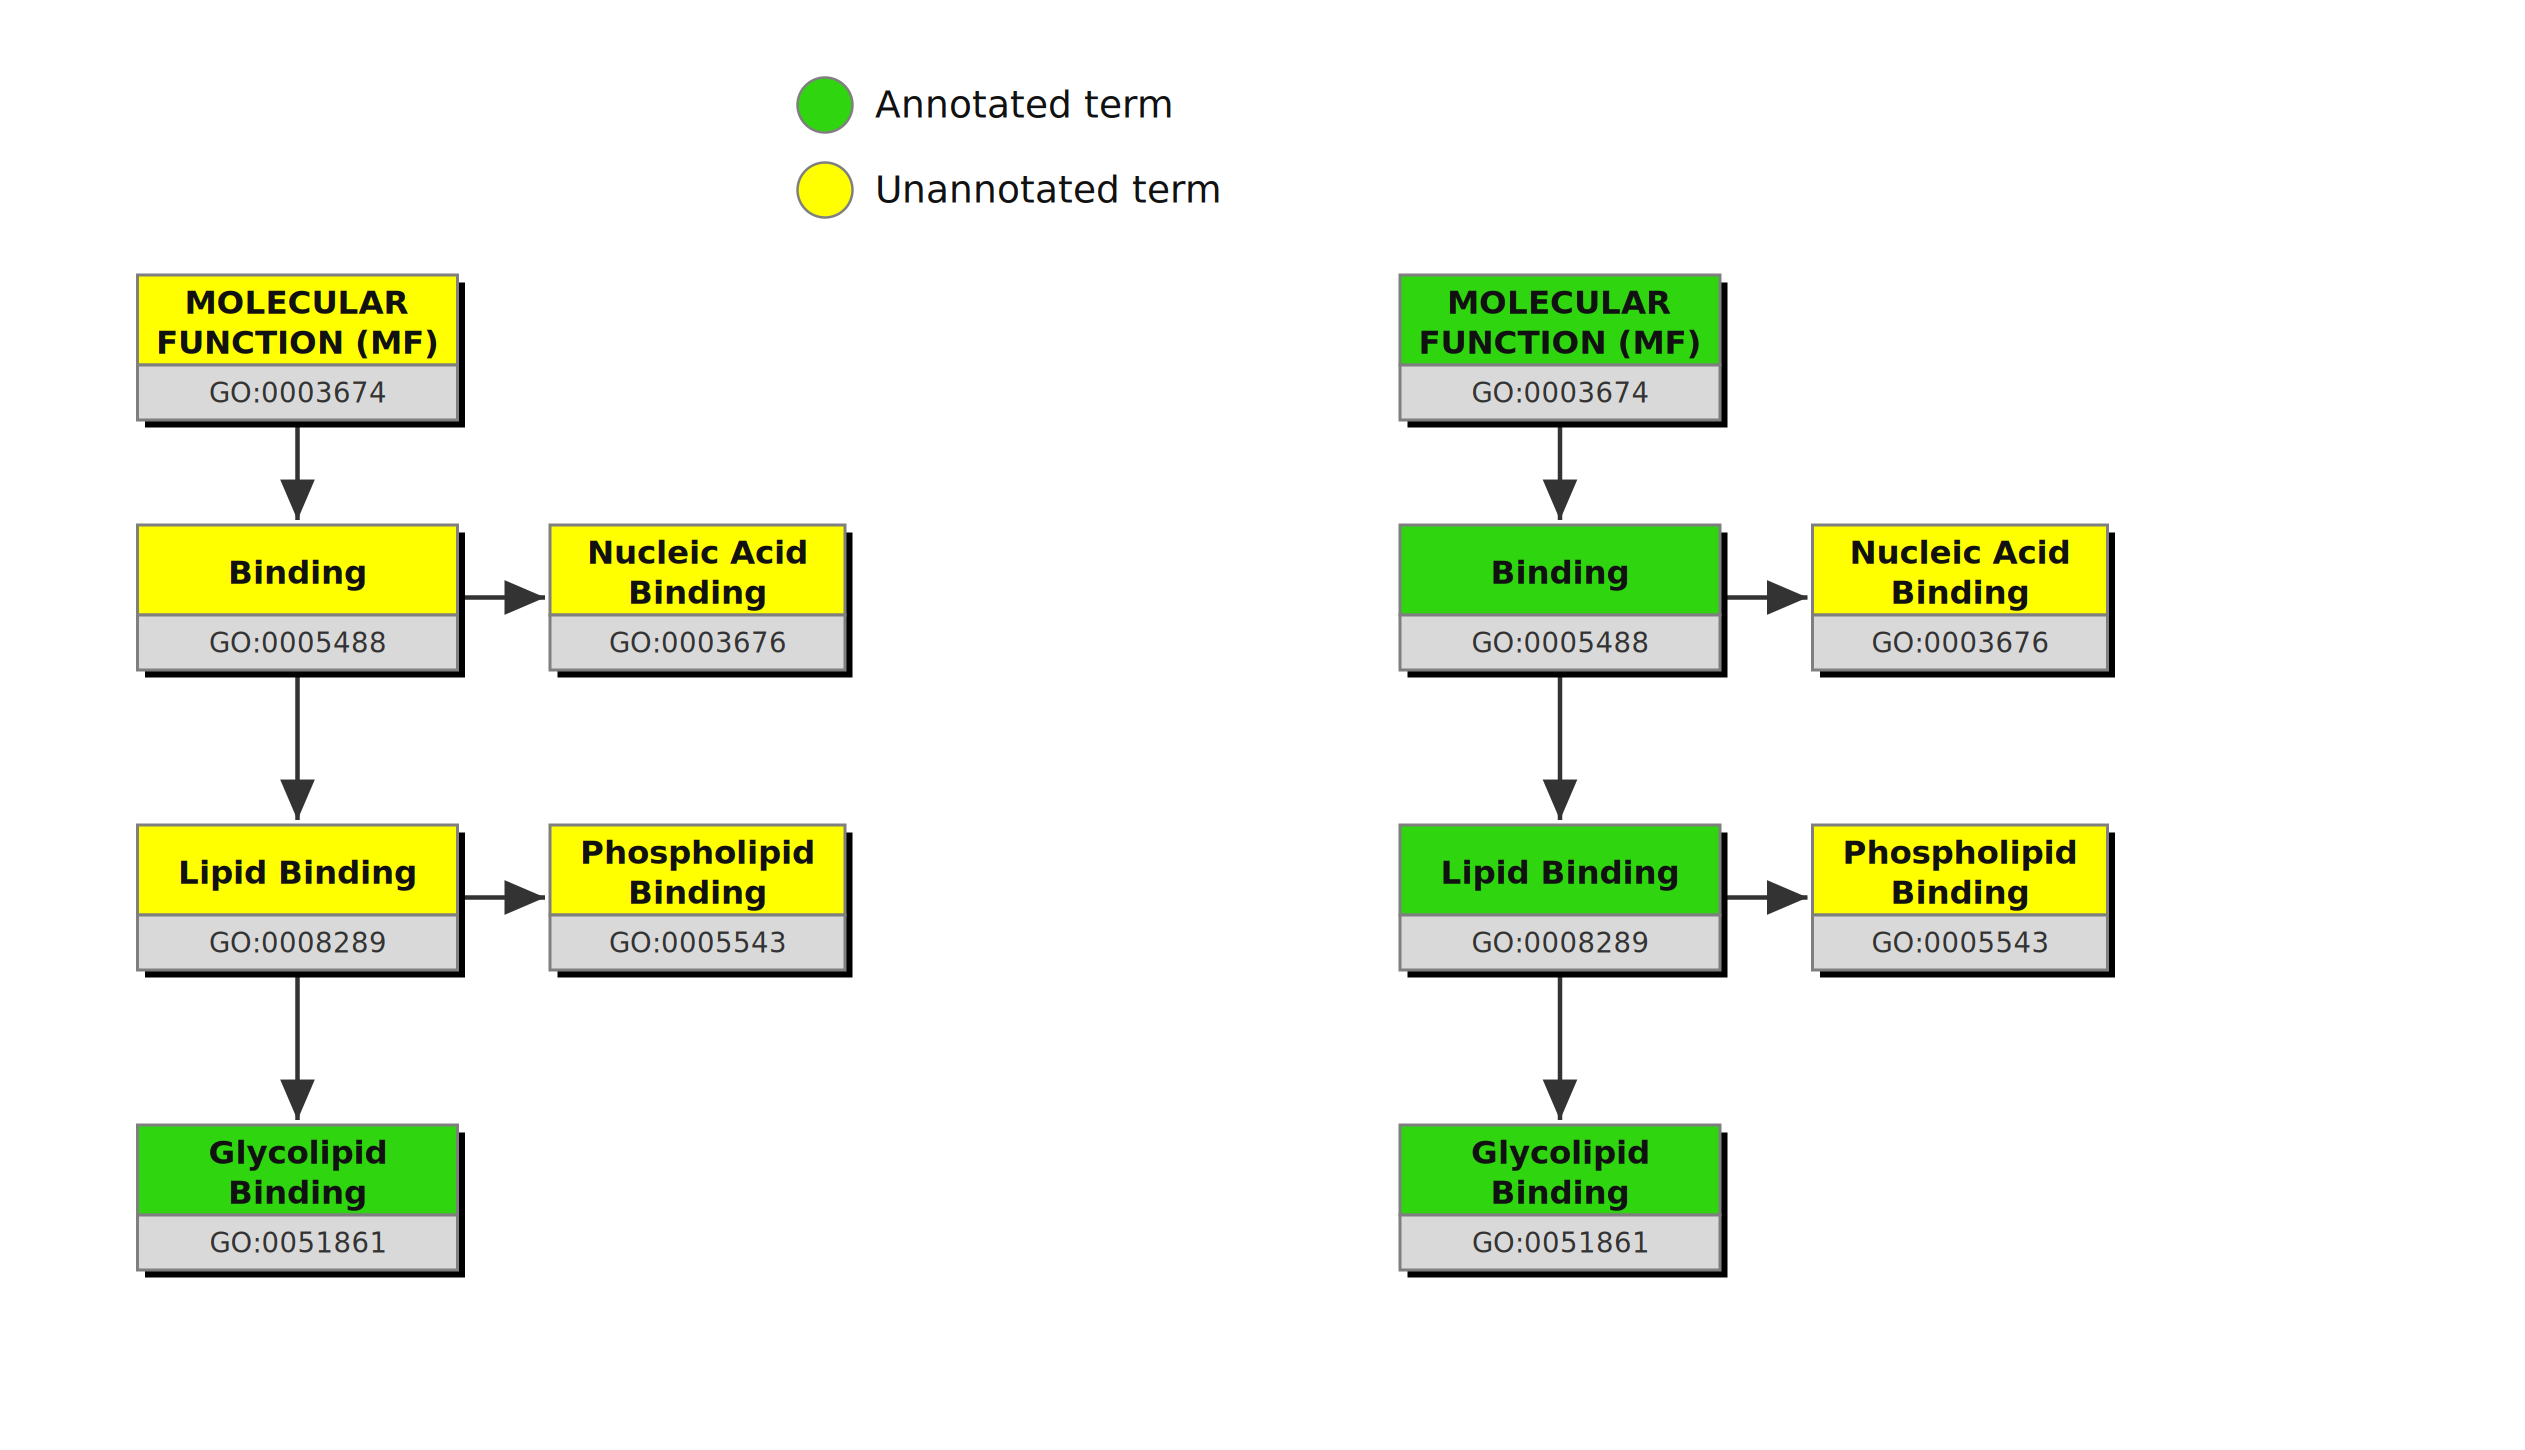
\includegraphics[width=\linewidth]{fig4_go_hierarchy_EN.png} 
    \caption{Illustration of the True Path Rule. Left: an inconsistent annotation, because a specific annotated term has unannotated ancestors. Right: a hierarchy-consistent annotation after propagation to the relevant ancestor terms.}
    \label{fig:ontology}
\end{figure}

The Gene Ontology is a dynamic resource that is continuously revised and expanded. As of the June 19, 2026 release, the official GO documentation reports the following numbers of valid terms: 10,052 for Molecular Function (MF), 4,075 for Cellular Component (CC), and 24,136 for Biological Process (BP). Because the ontology undergoes frequent updates (including the inclusion, modification, and obsolescence of terms), these statistics can quickly become outdated\footnote{\url{https://geneontology.org/stats.html}}.

\subsection{Protein-Protein Interaction Networks}


Proteins may establish stable or transient physical associations, including direct binding to form larger cooperative structures, such as the molecular complex illustrated in Figure~\ref{fig:complexo}~\cite{volonte2008protein, nepusz2012detecting}. In a computational context, these relationships are modeled as networks where nodes represent proteins and edges denote their interactions. However, the biological implication of an edge varies depending on the data source; while some networks strictly encode direct physical binding or co-complex membership, broader resources such as STRING also capture predicted functional associations between proteins participating in the same pathway or biological process~\cite{szklarczyk_string_2025}. While ``protein association network'' might more accurately describe the comprehensive nature of the data used in this study, the traditional acronym PPI (Protein-Protein Interaction) network is maintained throughout this text to align with established literature.

\begin{figure}[!htb]
    \centering
    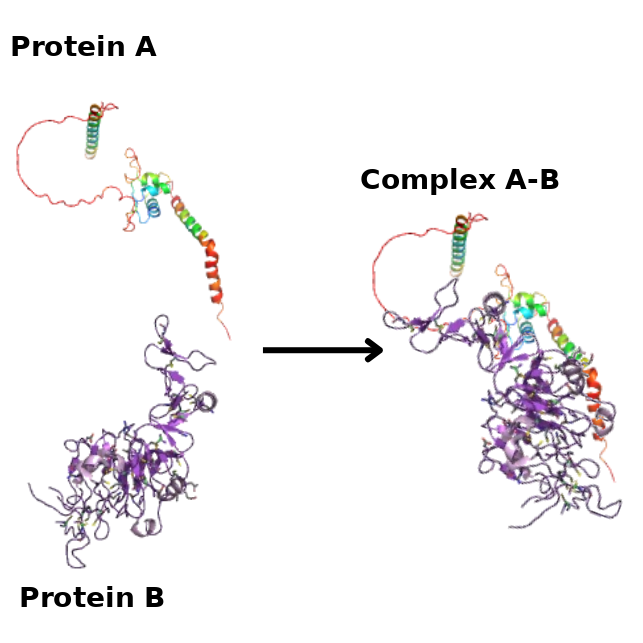
\includegraphics[width=0.5\linewidth]{fig1_protein_EN.png}
    \caption{Schematic example of a protein-protein interaction, illustrating the physical binding of two individual macromolecules (Protein A and Protein B) to form a functional multi-protein complex (Complex A-B).}
    \label{fig:complexo}
\end{figure}

To catalog these interactions, specialized databases gather evidence from diverse sources, though they differ slightly in scope and methodology. Resources such as BioGRID and IntAct primarily curate experimentally supported molecular interactions from the scientific literature. In contrast, STRING integrates these experimental records with computational channels, including gene neighborhood, gene fusion, co-expression, phylogenetic co-occurrence, and text mining~\cite{fields1989novel, safari-alighiarloo_protein-protein_2014, szklarczyk_string_2025}. The consolidation of this multi-channel information reflects both experimental observations and computational inferences, providing a comprehensive overview of functional complexes~\cite{raman_construction_2010}.

Each STRING edge is associated with a combined score that measures the confidence supported by the available evidence. This score should not be interpreted as binding affinity, interaction strength, stability, or magnitude of biological effect.

In co-immunoprecipitation (Co-IP), one example of an assay that generates experimental evidence of protein association, an antibody is used to isolate a target protein, and any proteins that co-purify with it typically belong to the same molecular complex under the evaluated conditions~\cite{kaboord2008isolation}. While this method strongly indicates complex formation, it does not strictly guarantee direct physical binding, as the association might be mediated by additional proteins. At the network level, the systematic analysis of these relationships allows function prediction models to rely on the guilt-by-association principle, which posits that connected proteins are statistically more likely to share functional roles. Although this correlation provides vital patterns for automated GO annotation, it acts as a probabilistic guideline rather than a deterministic rule, as the inference can be influenced by network incompleteness, multifunctional proteins, and highly connected hubs~\cite{valentini2010true, koh_analyzing_2012, gillis2011impact}.


\section{Computational Concepts}

In this section, we present the theoretical foundations of the computational methods employed in modeling, representation, and prediction in the field of bioinformatics.

\subsection{Graphs}

Graphs are fundamental mathematical structures used to model pairwise relations between objects. Formally, a graph is defined as $G = (V, E)$, where $V$ is the set of vertices (or nodes) and $E$ is the set of edges (or links) connecting them. In the context of computational biology and this dissertation, the STRING network is represented as a weighted graph $G = (V, E, w)$, in which each node represents a protein and $w : E \rightarrow \mathbb{R}_{>0}$ assigns a combined confidence score to each protein association from the PPI network.

To process graphs computationally, they must be translated into algebraic representations. The most direct approach is the adjacency matrix, denoted as $A \in \mathbb{R}^{N \times N}$, where $N = |V|$ is the total number of nodes. In an unweighted graph, $A_{ij} = 1$ if there is an edge between node $i$ and node $j$, and $0$ otherwise (see Figure~\ref{fig:generic_graph}). For weighted graphs, such as those derived from the STRING database~\cite{szklarczyk_string_2025}, $A_{ij}$ holds the confidence score of the interaction. Alongside the topological structure, each node typically possesses a set of attributes (e.g., protein sequence features), which are organized into a feature matrix $X \in \mathbb{R}^{N \times F}$, where $F$ is the feature dimensionality.

\begin{figure}[!htb]
    \centering
    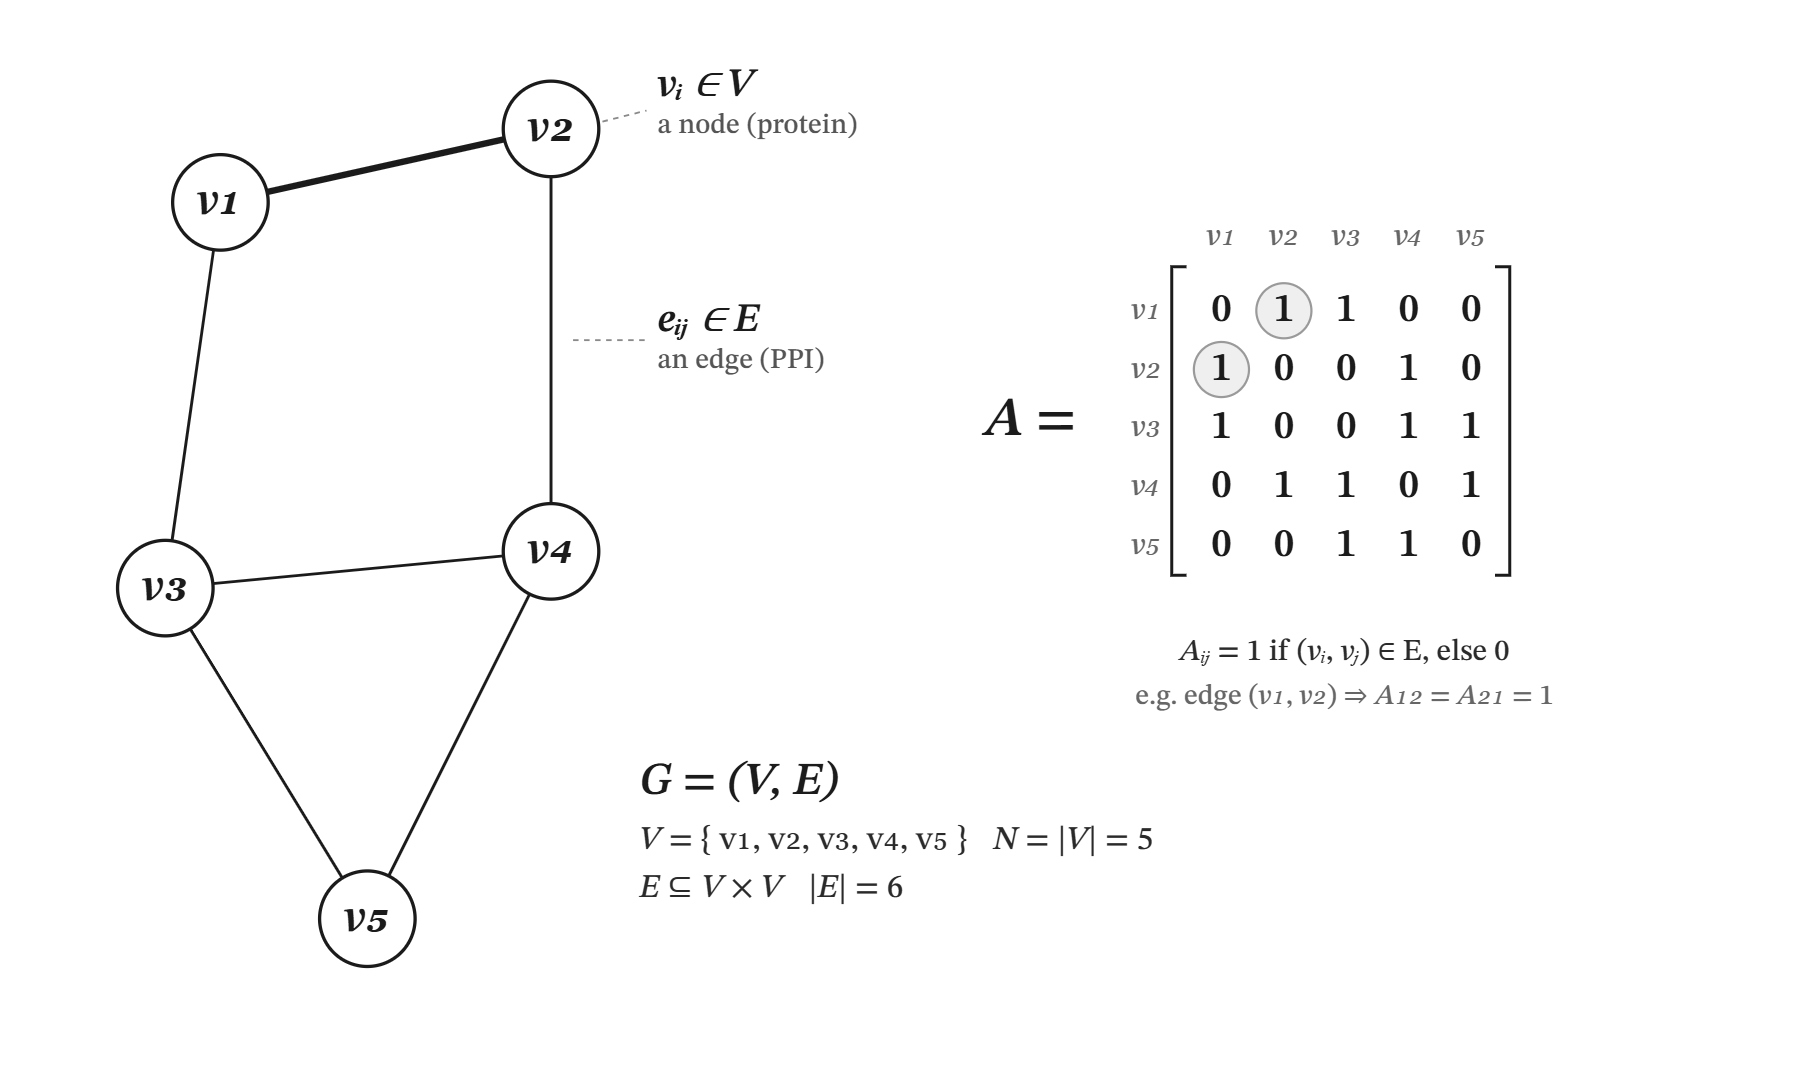
\includegraphics[width=\textwidth]{fig_graph_notation.png}
    \caption{A protein-protein interaction network modeled as a graph $G = (V, E)$: the vertices $V$ are proteins and the edges $E$ are PPIs. Its topology is encoded by the adjacency matrix $A \in \{0, 1\}^{N \times N}$, where $A_{ij} = 1$ whenever an edge connects nodes $v_i$ and $v_j$.}
    \label{fig:generic_graph}
\end{figure}

Large protein association networks are typically sparse, meaning that the number of non-zero entries in their adjacency matrix $A$ satisfies $|E| \ll N^2$. Storing $A$ as a dense matrix requires $O(N^2)$ memory, whereas sparse formats store only the non-zero entries and their indices. For example, the coordinate format (COO) stores a row index, a column index, and a value for each non-zero entry, reducing the graph-storage requirement to $O(|E|)$, apart from auxiliary indexing structures. Sparse representations are therefore preferable for large graphs, although dense representations may still be used for selected vectors, mini-batches, or transformed inputs.

Frameworks such as PyTorch Geometric (PyG)~\cite{fey2019fast} and the Deep Graph Library (DGL)~\cite{wang2019deep} provide essential data structures that facilitate the efficient implementation of message-passing algorithms and Graph Neural Networks. By highly optimizing sparse tensor operations on GPUs, these libraries enable the processing of massive biological networks. While these advancements drastically reduce computational overhead, scaling to full-graph training still requires careful consideration of graph size, feature dimensionality, and model depth. The specific framework and the training strategies employed to manage these variables are detailed in Chapter~\ref{cap:metodologia}.

\subsection{Machine Learning Paradigms}

Machine learning methods are traditionally categorized by their reliance on labeled data. In supervised learning, models are trained to map input features to explicit target labels. Unsupervised learning, in contrast, operates on entirely unlabeled data to uncover hidden structures, such as clusters or low-dimensional representations. Semi-supervised learning bridges this gap by combining a typically small set of labeled examples with a large volume of unlabeled data, leveraging the underlying data distribution to improve predictive performance~\cite{bishop2006pattern}.

In graph-based semi-supervised learning, labeled and unlabeled nodes coexist within the same graph. This allows the topology and attributes of all nodes to contribute to representation learning, while only the labels of the training nodes are used for optimization~\cite{kipf2017semi}. When predictions are generated for previously observed unlabeled nodes within this same graph, the setting is termed transductive. This corresponds to the exact graph setting adopted in this dissertation.

Within this semi-supervised transductive framework, protein function prediction is formally structured as a hierarchical multi-label classification task~\cite{tsoumakas2007multi}. Because a single protein is often involved in diverse biological processes, it must be capable of being assigned multiple Gene Ontology (GO) terms rather than a single exclusive class. The model's classification heads initially output independent probabilities for each retained term, after which hierarchical consistency is enforced using the directional structure of the GO, as detailed in Chapter~\ref{cap:metodologia}.

\subsection{Neural Networks and Deep Learning}

Artificial neural networks are composed of layers of parameterized units. During training, the model parameters (weights and biases) are updated using optimization algorithms (such as gradient descent) to reduce a loss function that measures the discrepancy between the predictions and the target labels~\cite{goodfellow2016deep}. Networks with multiple representation-learning layers are commonly referred to as deep neural networks.

\subsubsection{Simple Perceptron and the Decision Boundary}

The simple perceptron is the fundamental processing unit in various neural architectures. It performs a linear combination of the input attributes followed by the application of an activation function, defining a decision boundary. Mathematically, given the input attributes denoted by \(\mathbf{x} = (x_1, x_2, \ldots, x_n)\), the perceptron computes:
\begin{equation*}
\hat{y} = \sigma\bigl(\mathbf{w}^\top \mathbf{x} + b\bigr),
\end{equation*}
\noindent where \(\mathbf{w}\) are the weights, \(b\) is the bias, and \(\sigma(\cdot)\) is the activation function (Figure~\ref{fig:perceptron}). The classical perceptron uses a threshold activation and therefore defines a linear decision boundary. Modern neural networks typically use differentiable activation functions such as ReLU or sigmoid.

\begin{figure}[!htb]
    \centering
    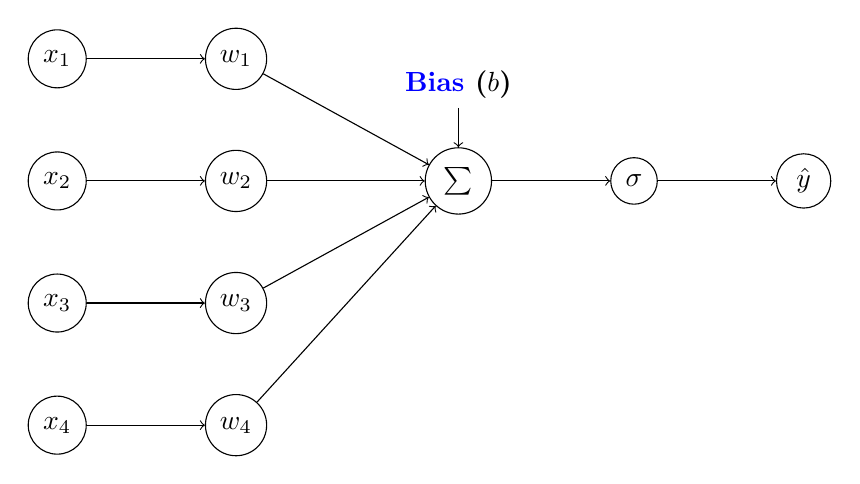
\begin{tikzpicture}
        % Input nodes
        \node[circle,draw] (x1)  {$x_1$};
        \node[circle,draw,below=0.8cm of x1] (x2) {$x_2$};
        \node[circle,draw,below=0.8cm of x2] (x3) {$x_3$};
        \node[circle,draw,below=0.8cm of x3] (x4) {$x_4$};

        % Weight nodes
        \node[circle,draw,right=1.5cm of x1] (w1) {$w_1$};
        \node[circle,draw,right=1.5cm of x2] (w2) {$w_2$};
        \node[circle,draw,right=1.5cm of x3] (w3) {$w_3$};
        \node[circle,draw,right=1.5cm of x4] (w4) {$w_4$};

        % Adder
        \node[circle,draw,right=2cm of w2] (sum) {\(\sum\)};

        % Bias
        \node[above=0.5cm of sum] (bias) {\textbf{\textcolor{blue}{Bias} ($b$)}};
        \draw[->] (bias) -- (sum);

        % Activation function
        \node[circle,draw,right=1.5cm of sum] (activation) {\( \sigma \)};

        % Output
        \node[circle,draw,right=1.5cm of activation] (yhat) {\(\hat{y}\)};

        % Connections
        \draw[->] (x1) -- (w1);
        \draw[->] (x2) -- (w2);
        \draw[->] (x3) -- (w3);
        \draw[->] (x4) -- (w4);

        \draw[->] (w1) -- (sum);
        \draw[->] (w2) -- (sum);
        \draw[->] (w3) -- (sum);
        \draw[->] (w4) -- (sum);

        % Network flow
        \draw[->] (sum) -- (activation);
        \draw[->] (activation) -- (yhat);
    \end{tikzpicture}
    \caption{Simple Perceptron Schematic.}
    \label{fig:perceptron}
\end{figure}

\subsubsection{Multilayer Perceptrons}

Multilayer Perceptrons (MLPs) consist of multiple fully connected layers (Figure~\ref{fig:mlp}). For neuron $j$ in layer $l$, the pre-activation $z_j^{(l)}$ and activation $a_j^{(l)}$ are given by:
\begin{equation*}
z_j^{(l)} = \sum_{i=1}^{n_{l-1}} W_{ji}^{(l)} a_i^{(l-1)} + b_j^{(l)}, \quad a_j^{(l)} = \sigma \left( z_j^{(l)} \right),
\end{equation*}
\noindent where $n_{l-1}$ is the number of units in the previous layer, $W_{ji}^{(l)}$ is the scalar weight connecting unit $i$ to unit $j$, $W^{(l)}$ is the corresponding weight matrix, and $b_j^{(l)}$ is the bias of unit $j$. During training, backpropagation computes the gradients of the loss with respect to the model parameters, and an optimizer such as Adam~\cite{kingma2015adam} uses these gradients to update the parameters and reduce the loss, seeking the direction of a local or global minimum, if it exists.

\begin{figure}[!htb]
    \centering
    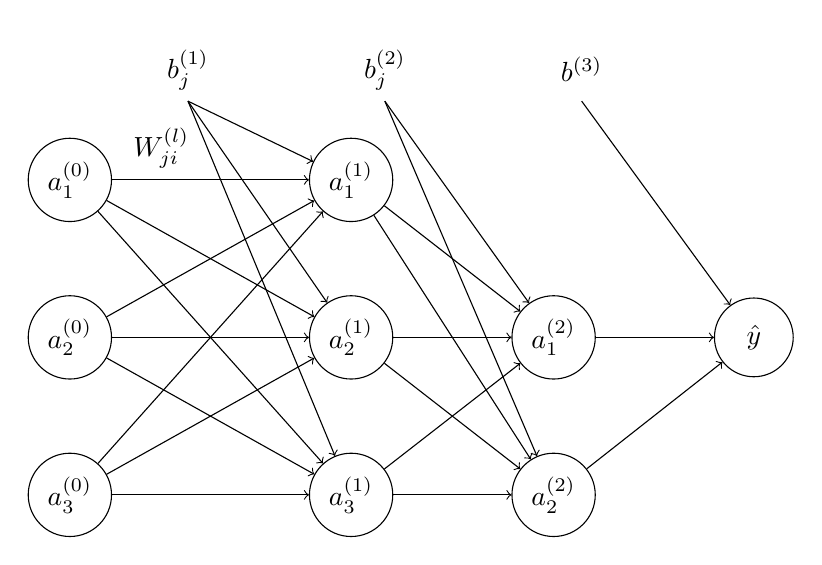
\begin{tikzpicture}[
        node distance=1cm and 1.5cm, 
        every node/.style={draw, circle, minimum size=1cm}
    ]

        % Input Layer
        \node (x1) at (0,2) {\(a_1^{(0)}\)};
        \node (x2) at (0,0) {\(a_2^{(0)}\)};
        \node (x3) at (0,-2) {\(a_3^{(0)}\)};
        
        % Hidden Layer 1 (Updated z -> a)
        \node[right=of x1, xshift=1cm] (h11) {\(a_1^{(1)}\)};
        \node[right=of x2, xshift=1cm] (h12) {\(a_2^{(1)}\)};
        \node[right=of x3, xshift=1cm] (h13) {\(a_3^{(1)}\)};
        
        % Hidden Layer 2 (Updated z -> a)
        \node[right=of h12] (h21) {\(a_1^{(2)}\)};
        \node[right=of h13] (h22) {\(a_2^{(2)}\)};
        
        % Output
        \node[right=of h21] (y) {\(\hat{y}\)};
        
        % Connections (Updated w_ij -> W_ji)
        \draw[->] (x1) -- node[near start, above, yshift=-2mm, draw=none] {\(W_{ji}^{(l)}\)} (h11);
        \draw[->] (x1) -- (h12);
        \draw[->] (x1) -- (h13);
        
        \draw[->] (x2) -- (h11);
        \draw[->] (x2) -- (h12);
        \draw[->] (x2) -- (h13);
        
        \draw[->] (x3) -- (h11);
        \draw[->] (x3) -- (h12);
        \draw[->] (x3) -- (h13);
        
        \foreach \i in {1,2,3} {
            \foreach \j in {1,2} {
                \draw[->] (h1\i) -- (h2\j);
            }
        }
        
        \foreach \i in {1,2} {
            \draw[->] (h2\i) -- (y);
        }
        
        % Biases
        \foreach \i in {1,2,3} { \draw[->] (1.5,3) -- (h1\i); }
        \foreach \i in {1,2} { \draw[->] (4,3) -- (h2\i); }
        \draw[->] (6.5,3) -- (y);
        
        \node[draw=none] at (1.5,3.4) {\(b_j^{(1)}\)};
        \node[draw=none] at (4,3.4) {\(b_j^{(2)}\)};
        \node[draw=none] at (6.5,3.4) {\(b^{(3)}\)};

    \end{tikzpicture}
    \caption{Architecture of an MLP with two hidden layers.}
    \label{fig:mlp}
\end{figure}


\subsubsection{Convolutional Neural Networks}

Convolutional Neural Networks (CNNs) exploit local structure in regularly organized data, including one-dimensional sequences and two-dimensional images~\cite{rawat2017deep}. Convolutional filters (kernels) share parameters across positions to extract local patterns (such as edges and textures) and produce translation-equivariant feature maps. Pooling or global aggregation may subsequently provide a degree of robustness or approximate invariance to small translations.

A CNN typically alternates convolutional transformations, nonlinear activations, normalization, and optional downsampling operations. The resulting representation may be flattened or globally pooled before being processed by a classification layer (Figure~\ref{fig:conv_layer_fluxo}).

\begin{figure}[!htb]
    \centering
    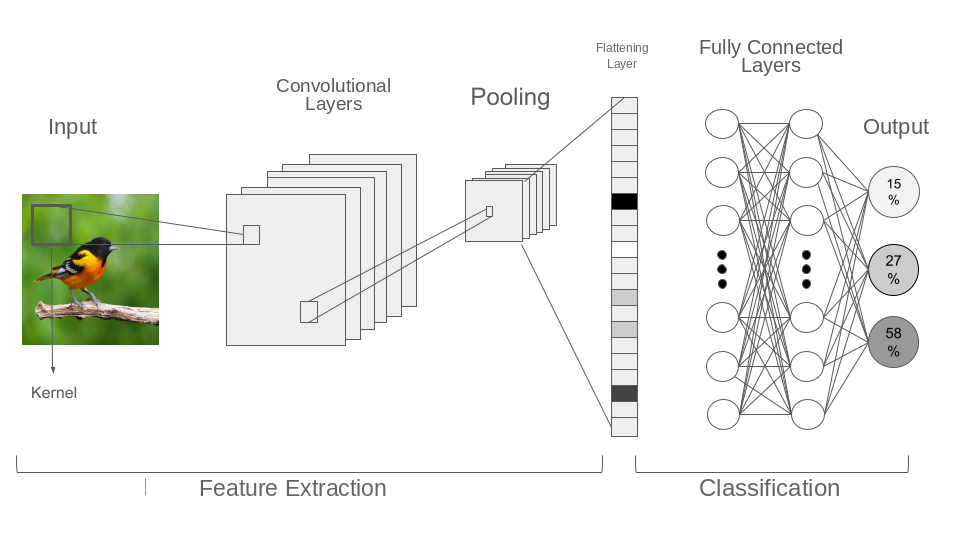
\includegraphics[width=0.96\textwidth]{fig2_cnn_EN.png}
    \caption{Generic convolutional classification pipeline comprising convolutional feature extraction, spatial downsampling, representation aggregation, and a final classification head.}
    \label{fig:conv_layer_fluxo}
\end{figure}

\subsubsection{Graph Neural Networks}

The feature extraction capabilities of convolutions, widely consolidated in regular Euclidean data by CNNs, can also be extended to complex irregular structures. Since multiple biological domains, particularly PPI networks, are intrinsically organized as graphs, Graph Neural Networks (GNNs) transpose the convolution concept to these non-Euclidean spaces through a framework known as message passing~\cite{kipf2017semi, gilmer2017neural}.

In this framework, GNNs learn latent node representations by repeatedly exchanging and aggregating information along graph edges. In a message-passing layer $l$, node $v$ first aggregates messages from its immediate neighbors:
\begin{equation*}
m_v^{(l)} = \text{AGG}^{(l)} \left( \left\{ \phi^{(l)} \left( h_v^{(l)}, h_u^{(l)}, e_{uv} \right) : u \in \mathcal{N}(v) \right\} \right),
\end{equation*}
\noindent and then updates its representation:
\begin{equation*}
h_v^{(l+1)} = \psi^{(l)} \left( h_v^{(l)}, m_v^{(l)} \right),
\end{equation*}
\noindent where $h_v^{(l)}$ is the vector representation of node $v$, and $\mathcal{N}(v)$ denotes its connected neighborhood. The function $\text{AGG}^{(l)}$ represents a permutation-invariant aggregator (such as a sum, mean, or maximum operation), $\phi^{(l)}$ defines the message computation, and $\psi^{(l)}$ defines the node update. In the context of PPIs, the edge attribute $e_{uv}$ may incorporate probabilistic confidence scores provided by repositories such as STRING~\cite{szklarczyk_string_2025}.

A single message-passing layer incorporates information exclusively from a node's immediate neighbors. Consequently, by stacking $L$ successive layers, the network effectively expands its receptive field, allowing topological information to propagate through paths of up to $L$ edges, thereby capturing structural dependencies from an $L$-hop neighborhood.

Two message-passing architectures evaluated in this dissertation are:

\begin{itemize}
    \item \textbf{Graph Convolutional Networks (GCNs):} The GCN proposed by Kipf and Welling~\cite{kipf2017semi} aggregates neighboring representations using a symmetrically normalized adjacency matrix. After adding self-loops, the contribution associated with an edge $(i, j)$ is scaled according to $1/\sqrt{\tilde{d}_i\tilde{d}_j}$, where $\tilde{d}_i$ and $\tilde{d}_j$ are the corresponding node degrees. This operation performs a normalized neighborhood smoothing followed by a learnable linear transformation.
    
    \item \textbf{Graph Attention Networks (GATs):} GATs learn attention coefficients that assign different relative weights to neighboring nodes during aggregation~\cite{velickovic2018graph}. This mechanism allows the model to emphasize some neighbors over others, although it does not guarantee that noisy edges will receive lower weights.
\end{itemize}

Full-graph GNN training can require substantial RAM or GPU memory because node representations and intermediate activations must be maintained across a large number of edges. The cost depends on the graph size, feature dimensionality, number of layers, and training strategy. Increasing the number of message-passing layers also enlarges the receptive field, but excessive propagation may make neighboring node representations increasingly similar, a phenomenon commonly referred to as oversmoothing. These computational and representational limitations motivate the comparison with the fixed non-parametric propagation method introduced in Chapter~\ref{cap:metodologia}.

\subsection{Self-Supervised Learning}

Self-supervised learning~\cite{liu2021self} constructs training targets directly from the input data, eliminating the need for manually assigned labels during pretraining. Depending on the data modality, common objectives include predicting masked elements, reconstructing corrupted inputs, or contrasting related and unrelated examples~\cite{jing2020self}.

One foundational architecture for this paradigm is the autoencoder. It is typically structured into two main components: an encoder, which maps high-dimensional input data into a latent representation (often acting as a bottleneck for dimensionality reduction and feature extraction), and a decoder, in charge of reconstructing the original input from this latent space (Figure~\ref{fig:autoencoder_diagrama}).

\begin{figure}[!htb]
    \centering
    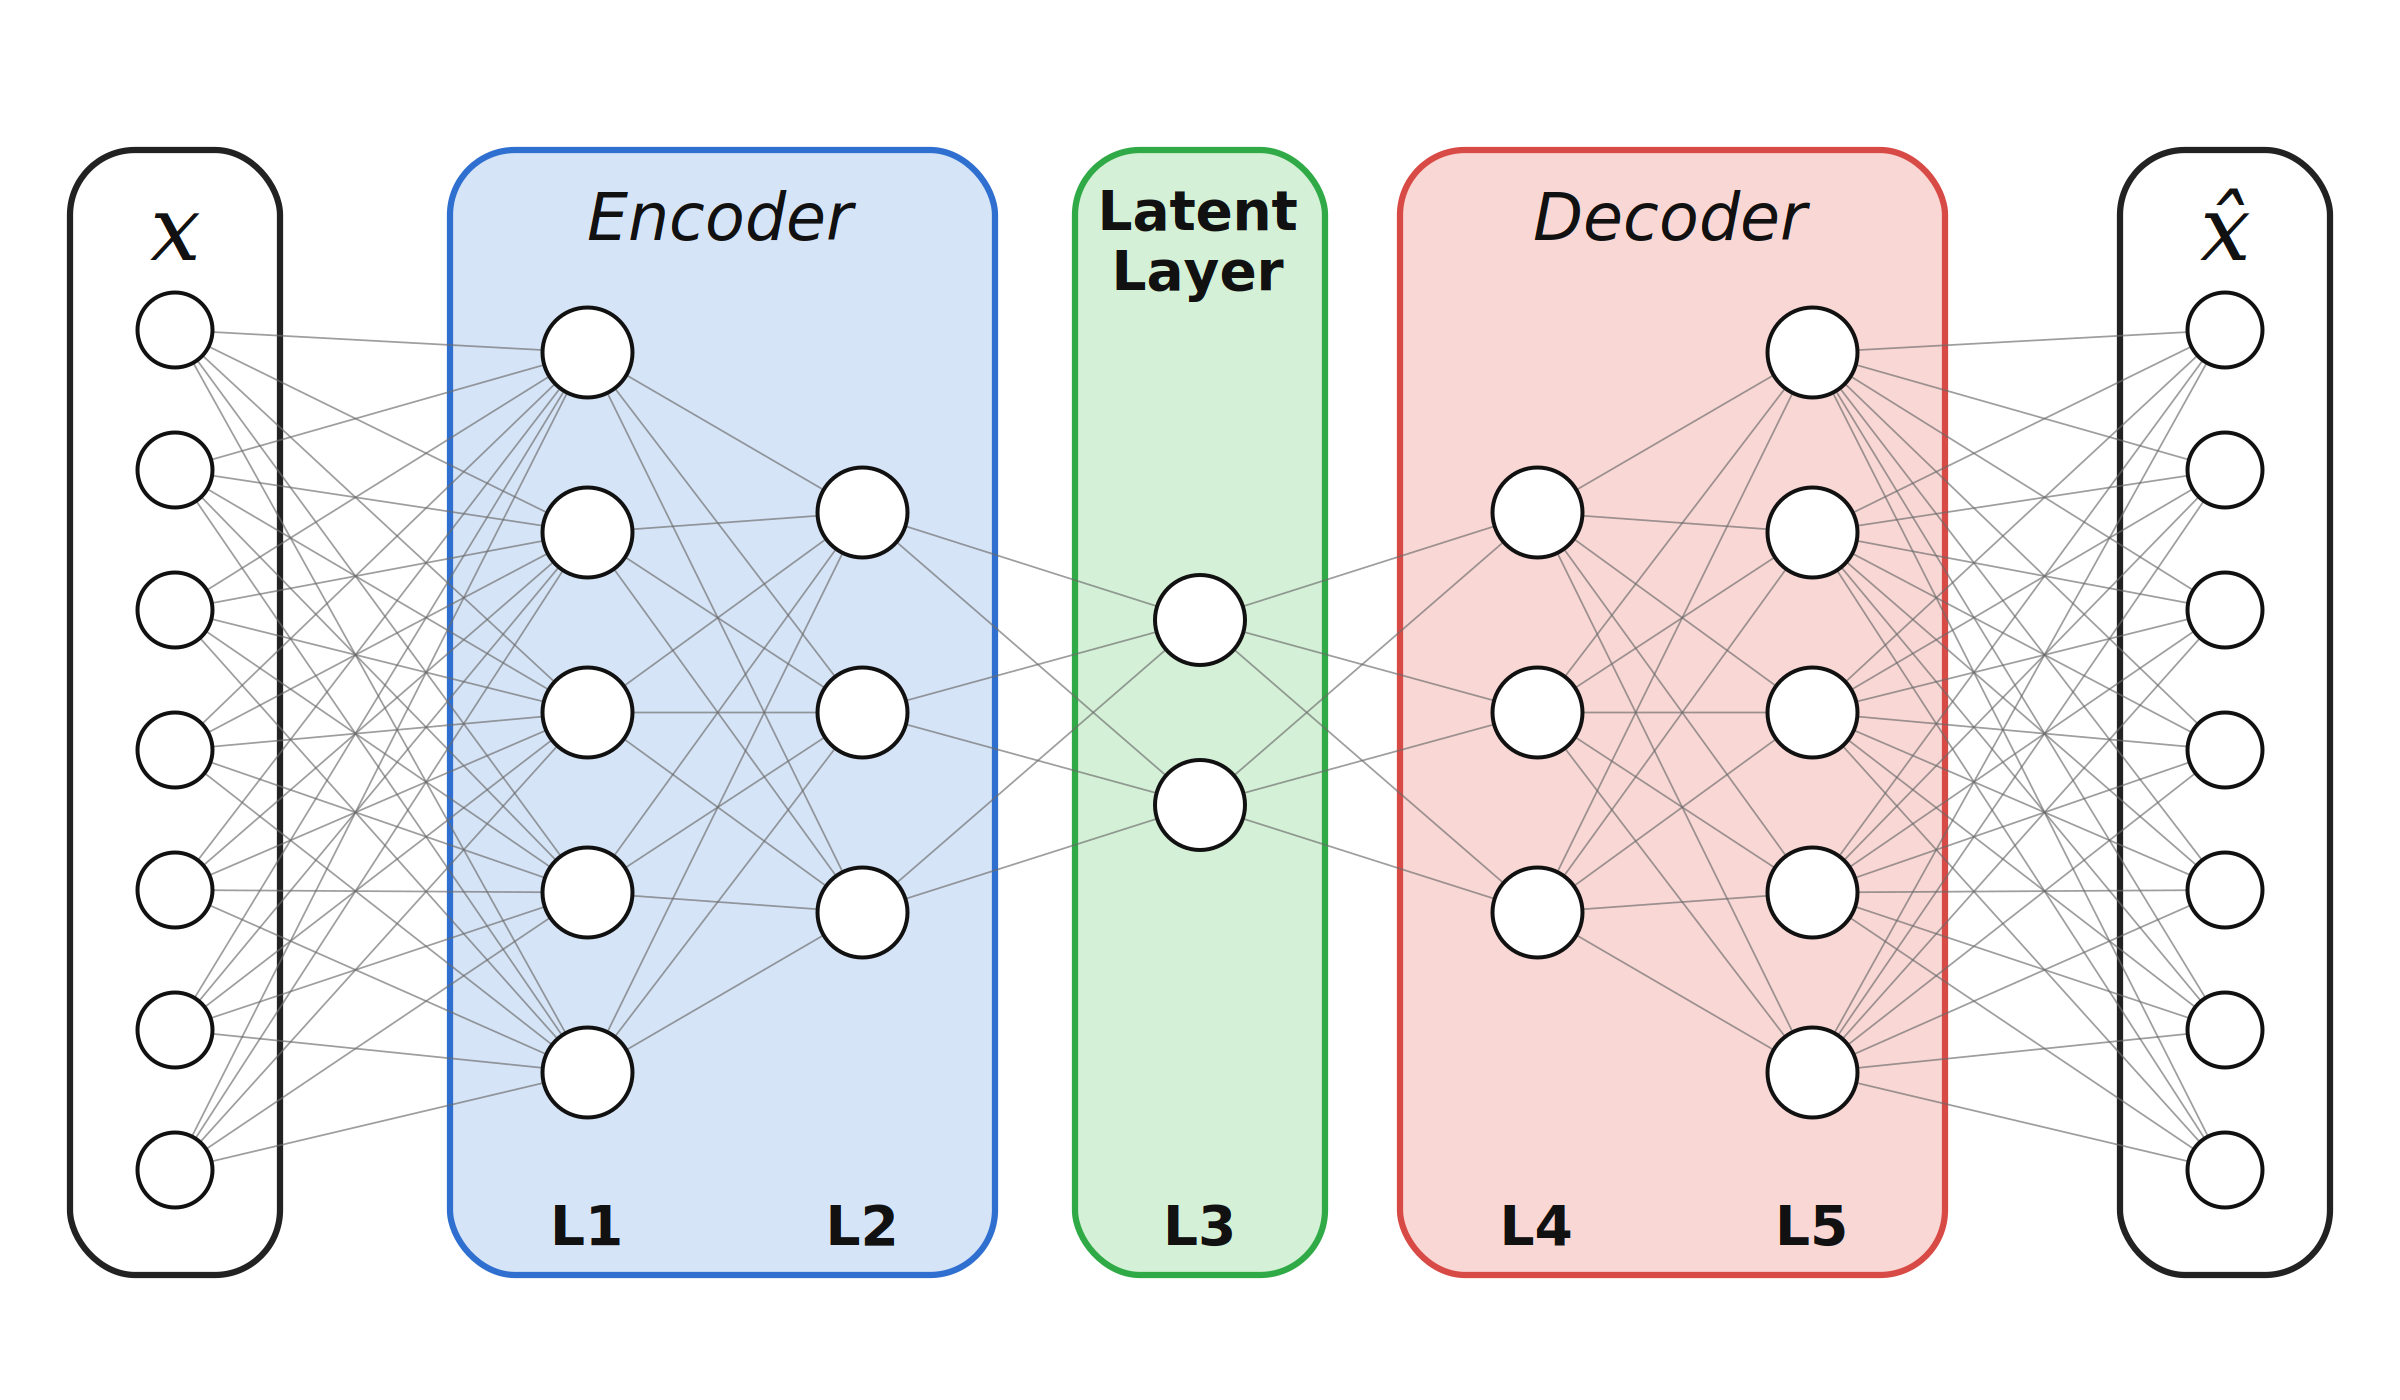
\includegraphics[width=0.8\textwidth]{fig3_autoencoder_EN.png}
    \caption{Schematic of an Autoencoder architecture, showing latent encoding for dimensionality reduction and the subsequent reconstruction.}
    \label{fig:autoencoder_diagrama}
\end{figure}

In the scope of contrastive learning, models are optimized to maximize the similarity in the latent space between positive pairs (such as two different stochastic augmentations of the same original sample) and repel negative pairs (independent or disparate instances)~\cite{chen2020simple}. The representations resulting from these diverse self-supervised approaches can subsequently be used as fixed feature extractors or fine-tuned for supervised downstream tasks.

For sequence models, self-supervised objectives commonly require the prediction or reconstruction of masked or corrupted tokens using their surrounding context. Protein language models apply analogous objectives to amino-acid sequences to produce rich contextual representations~\cite{elnaggar2021prottrans}. In this dissertation, ProtT5 is utilized specifically as a fixed feature extractor: its encoder representations are precomputed from the protein sequences and subsequently used as static node attributes in the PPI graph.

\subsection{Attention Mechanism and Transformers}

Traditionally, the processing of sequential data (such as natural language texts or time series) was heavily reliant on recurrent neural networks (RNNs) and their variants (like LSTMs~\cite{hochreiter1997long}). Although LSTMs were specifically designed to mitigate difficulties with long-range dependencies, these networks inherently process information in a strictly sequential manner. This recurrent nature makes parallelization across positions difficult, and retaining context over very long sequences remains challenging.

Methodological advances have addressed these limitations through attention mechanisms, which provide direct, content-dependent connections between sequence positions. Among the variations of this mechanism, self-attention stands out by allowing the model to dynamically and in parallel compute the importance of each element relative to all others, regardless of their positional distance. However, because self-attention alone does not capture token order, positional information must be incorporated separately. Furthermore, while it enables greater parallelism during training, this global comparison introduces a computational cost that scales quadratically with the sequence length.

Vaswani et al.~\cite{vaswani2017attention} introduced the original Transformer as an encoder–decoder architecture based primarily on attention mechanisms. The two components are:
\begin{itemize}
    \item \textbf{Encoder:} transforms the input sequence into a sequence of contextualized representations using self-attention and feed-forward layers. Because each input position can attend to all other input positions, the resulting representations incorporate bidirectional context.
    \item \textbf{Decoder:} generates the output autoregressively using causal self-attention over previously generated tokens and cross-attention over the encoder representations.
\end{itemize}

The Transformer architecture gave rise to several model families. Encoder–decoder models, such as T5~\cite{raffel2020exploring}, are designed for sequence-to-sequence tasks. Decoder-only models, such as the GPT family, use causal attention and are commonly trained for autoregressive generation. Encoder-only models, including BERT, RoBERTa, and ELECTRA~\cite{devlin2019bert, liu2019roberta, clark2020electra}, produce contextualized representations that are frequently transferred to classification and representation-learning tasks. XLNet~\cite{yang2019xlnet} does not belong to the encoder–decoder category; it is a generalized autoregressive model based on Transformer-XL and trained with a permutation language-modeling objective that allows it to capture bidirectional context.

Regardless of the specific branch, these model families are commonly pretrained on large unlabeled corpora using self-supervised objectives, although the objective and model size vary across architectures. Examples include causal language modeling, masked-token prediction, span corruption, replaced-token detection, and permutation language modeling. After pretraining, the hidden representations may be extracted as fixed embeddings or the model parameters may be fine-tuned for a downstream task.

In the domain of computational biology, this methodological foundation gave rise to the so-called protein language models (PLMs). These models adapt self-supervised sequence modeling to proteins by treating an amino-acid sequence as a sequence of discrete tokens. During pretraining on large protein sequence corpora, such as UniRef\footnote{\url{https://www.uniprot.org/help/uniref/}} and UniProt\footnote{\url{https://www.uniprot.org/}}, the models learn statistical regularities that can be transferred to downstream biological tasks~\cite{elnaggar2021prottrans}.

Relevant PLM families include ProtBERT and ProtT5 from the ProtTrans project, as well as the ESM models. ProtBERT and ESM models use encoder-based architectures, whereas ProtT5 is based on the T5 encoder–decoder architecture~\cite{elnaggar2021prottrans}. For representation extraction, the amino-acid sequence is processed by the model and the per-residue encoder states are aggregated into a fixed-dimensional protein embedding. Such embeddings have been shown to encode information useful for predicting structural, evolutionary, and functional properties, making them suitable node attributes for graph-based modeling. In this dissertation, the ProtT5 embeddings are stored in the node-feature matrix $X$ and subsequently propagated over the STRING graph.


\subsection{Transfer Learning}

Transfer learning exploits the weights of massive neural models previously trained on exhaustive datasets (such as the global ImageNet corpus~\cite{russakovsky2015imagenet} for vision or protein sequence repositories for PLMs) to initialize a network for a specific secondary task. 

This reuse of knowledge typically follows two main approaches. In feature extraction, the pretrained model is kept entirely frozen, and its outputs serve as static inputs for a newly trained downstream predictor. In fine-tuning approaches, some or all of the pretrained parameters are selectively updated using the target data. Both strategies allow for much faster convergence and help avoid severe overfitting on restricted labeled datasets, although their ultimate effectiveness strongly depends on the similarity between the source and target domains.

\subsection{Classifier Combination}

Ensemble methods combine multiple predictors or representations with the goal of improving predictive performance or stability~\cite{dietterich2000ensemble}. An ensemble is most likely to be beneficial when its component models are individually informative and make complementary errors; combining models does not by itself guarantee an improvement over the strongest component.

In protein function prediction, sequence-based and graph-based models may capture different aspects of the data. Feature-level or early-fusion methods combine intermediate representations before the final classifier, for example through concatenation or element-wise operations. Prediction-level or late-fusion methods combine the outputs of independently trained models using operations such as averaging, weighted averaging, maximum selection, or a learned meta-classifier. In stacking, held-out or out-of-fold base-model predictions are normally used to reduce overfitting and avoid leakage from the base models' training targets. Chapter~\ref{cap:metodologia} describes the specific early- and late-fusion strategies evaluated in this dissertation.

\chapter{Literature Review and Related Work}
\label{cap:trabalhos}

This chapter reviews the computational literature on protein function prediction and situates the
present work within it. The concepts on which the reviewed methods rest were introduced in
Chapter~\ref{cap:fundamentacao} and are recalled below only where a method's assumptions depend on them;
the emphasis falls on how each family operates and on what those assumptions cost.

\section{The Evolution of Approaches to Functional Annotation}
\label{sec:rel_evolucao}

The account that follows is organized by the evidence a method consumes rather than strictly by
chronology, although the two orders largely coincide. It begins with the descriptors computed for a
protein in isolation, from sequence alignment and domain composition to protein language model
representations, and turns next to the methods whose only input is the interaction network. It closes
with the hybrid family that combines the two, which is where the present proposal is situated and
where its immediate precedents are found.

\subsection{From Experimental Characterization to Automated Annotation}
\label{sec:rel_classicos}

Given the annotation asymmetry described in Chapter~\ref{cap:introducao}, the question that has organized
the field for over a decade is not whether prediction is possible but how it should be measured. The
Critical Assessment of Functional Annotation settled it in practice, scoring methods on proteins
whose experimental characterization was not yet public~\cite{radivojac2013large} and consolidating
the metrics the field now treats as standard~\cite{zhou_cafa_2019}. The methods reviewed below were,
with few exceptions, designed against that target.

The assessment of the fifth Critical Assessment of Functional Annotation has since been reported, providing a prospective, time-delayed evaluation of the methods submitted to CAFA5 under shared target and metric definitions. The assessment documents continued progress in protein function prediction while also showing that relative performance depends on the ontology, target population, metric, and prediction coverage. Although the corpus used in this dissertation is derived from CAFA5 training material, the present experiments do not reproduce the official CAFA5 benchmark: they use an internal random protein-level partition and a transductive graph, and therefore answer a different experimental question~\cite{depaoliskaluza2026cafa5}.

The oldest automated route is transfer by sequence similarity. The BLAST family locates high-scoring
local alignments between a query and a database, and PSI-BLAST iterates the search with
position-specific scoring matrices derived from the previous round, which extends its reach to more
remote relationships~\cite{altschul1997gapped}. Its limitation is inferential rather than
computational: below the classical twilight-zone range, whose practical boundary depends on
alignment length, composition and statistical significance, sequence identity alone becomes an
unreliable indicator of homology and structural similarity~\cite{rost1999twilight}. Functional
transfer is more delicate still, because homologous proteins may retain a fold while diverging in
substrate specificity or biological role, and transfer also propagates whatever errors the source
annotation contains. A complementary descriptor is domain composition, where profile hidden Markov
models detect occurrences far below that threshold and InterPro integrates the signatures of a dozen
member databases~\cite{blum2025interpro}; it is the form in which DeepGraphGO and SEGT-GO represent
their proteins, at the cost of rendering identical domain architectures indistinguishable. Structure
enlarged the available evidence without closing the gap: AlphaFold raised structure prediction to
near-experimental accuracy at the level of individual domains in the CASP14
assessment~\cite{jumper2021alphafold}, but a confident fold is a scaffold rather than a mechanism,
and promiscuous folds transfer the same ambiguity one level up.

The change with the widest effect on this task came from self-supervised protein language models.
Trained on hundreds of millions of unaligned sequences, models of the ProtTrans and ESM families
produce dense representations encoding biochemical, structural and evolutionary regularities without
an alignment step~\cite{elnaggar2021prottrans,rives2021esm1b}, so that function prediction becomes
ordinary multi-label classification over a fixed-length vector.

Predictors then developed along two tracks. One retained an explicit sequence encoding, as in
DeepGOPlus, which combines convolutional motif detectors over one-hot encoded residues with an
alignment-based component and uses no language-model representation~\cite{kulmanov2020deepgoplus}.
The other consumed those representations directly, as in InterLabelGO+, which models correlations
among Gene Ontology terms and weights its objective by information
content~\cite{liu2024interlabelgo}; the composite protein-centric objective introduced there is the
one adopted in Chapter~\ref{cap:metodologia}. What the two tracks share, with the classical methods
before them, is that each describes a protein in isolation: these descriptors are computed from the
protein alone, without explicit use of its interaction neighborhood. They may nevertheless encode
sequence constraints associated with interaction or cellular context, but they do not observe those
relationships directly. Function is only partly intrinsic, most visibly for the aspects whose labels
name a role in a system rather than a chemical capability, and the remainder of this chapter
therefore concentrates on the methods that exploit interaction networks.

\subsection{Network-Based Methods: From Neighborhood Voting to Graph Embeddings}
\label{sec:rel_redes}

The guilt-by-association principle described in Chapter~\ref{cap:fundamentacao} admits many computational
readings, and the history of this branch is largely the history of making that reading progressively
less local. The earliest formulations are the most direct: Vazquez et al.~\cite{vazquez_global_2003}
assign to each unannotated protein the function most frequent among its partners, posed as a global
optimization over the network rather than as an independent decision per protein. Sharan, Ulitsky and
Shamir~\cite{sharan2007network} divide this first generation into direct annotation schemes, which
transfer labels across edges, and module-assisted schemes, which annotate detected modules as a unit.
The direct reading remains competitive when the network is informative:
Piovesan et al.~\cite{piovesan2015protein} report that Gene Ontology enrichment over the STRING
partners of a query outperforms an optimized BLAST baseline for two of the three domains.

Neighborhood voting reads only the first ring, and diffusion generalizes it. The semi-supervised
formulation of Zhou et al.~\cite{zhou2004learning} spreads label information iteratively while
restoring at each step a fixed fraction of the initial label assignment, so that influence decays
with distance instead of being truncated at a fixed radius; the same restart device reappears in
personalized-PageRank propagation~\cite{klicpera2019predict}. A related but distinct construction
retains a fraction of the current state rather than of the initial one, which yields a lazy
random-walk operator applied for a finite number of steps. Because it never reintroduces the initial
state, it does not share the personalized fixed point of the restart formulations, and the retention
coefficient slows the mixing instead of anchoring the result to the initial assignment;
Chapter~\ref{cap:metodologia} adopts this construction, so the distinction is consequential rather
than notational. Its counterpart on the feature side is the random walk with restart, in which a
walker moves along edges and returns to its origin with fixed probability, yielding for each node a
stationary distribution over the whole graph~\cite{tong2006fast}.

A second shift then replaced the propagation of labels by the propagation of representations. The
family originates in DeepWalk, which samples truncated random walks and trains a skip-gram model so
that nodes co-occurring in walks receive similar vectors~\cite{perozzi2014deepwalk}, and continues in
node2vec, whose second-order biased walk interpolates through two parameters between breadth-first
and depth-first exploration, associated respectively with structural equivalence and community
homophily~\cite{grover2016node2vec}. The relation to matrix factorization is closer than the
formulations suggest, since DeepWalk, LINE and node2vec all factorize closed-form matrices built from
powers of the transition matrix~\cite{qiu2018network}. A third route dispenses with the skip-gram
objective entirely: multi-step co-occurrence counts accumulated by a random walk are converted into a
positive pointwise mutual information matrix and compressed by a neural encoder~\cite{cao2016deep},
which is the preprocessing deepNF adopts. Granularity is worth keeping in view when reading this
family, since graph2vec, despite the name, produces a single vector per graph from
Weisfeiler-Lehman rooted subgraphs and is evaluated on graph
classification~\cite{narayanan2017graph2vec}; it operates one level above the others and cannot label
individual proteins inside a single large interaction network.

The costs of this family follow from its only input. Gillis and Pavlidis~\cite{gillis2011impact}
showed that guilt-by-association benchmarks are substantially inflated by multifunctional genes and
by node degree, so a method exploiting connectivity alone can appear to succeed without learning
anything specific to the function predicted. Coverage is the second cost: the reference map of the
human binary interactome covers an estimated two to eleven percent of the true interactome and
returns no interaction for roughly half of the proteins assayed~\cite{luck2020reference}. That figure
characterizes a single-species binary screen rather than an aggregated-evidence resource of the kind
used in this work, but the qualitative consequence carries over: a representation defined exclusively
by topology is undefined wherever topology is absent, and the isolation rate observed on the present
corpus is reported in Chapter~\ref{cap:materiais}.

\subsection{Hybrid Approaches and the Era of Graph Neural Networks}
\label{sec:rel_gnn}

The natural response is to stop asking the network to serve as the representation and to ask it
instead to modify a representation obtained elsewhere. DeepGO expressed this early, combining
sequence-derived features with interaction information under a classifier aware of the ontology
structure~\cite{kulmanov2018deepgo}. Later work extended the idea to networks whose node attributes
already carry sequence, localization and domain information. Graph2GO embeds one variational graph
autoencoder per attribute modality and concatenates the results~\cite{fan2020graph2go}, while CFAGO
pretrains a transformer autoencoder to reconstruct both the adjacency and the attribute matrix before
fusing the two through multi-head attention~\cite{wu2023cfago}. In each case the network contributes
context to a descriptor that exists independently of it, which is the structural difference
separating this family from the previous one.

The line matured alongside the adoption of graph neural networks, and two of their properties bear
directly on what follows. The first is the observational regime, since node classification on graphs
is usually posed transductively while GraphSAGE introduced the inductive alternative in which the
aggregation function generalizes to vertices absent at training
time~\cite{yang2016revisiting,hamilton2017graphsage}, a distinction that determines whether two
methods evaluated on the same corpus are solving the same problem. The second is cost: each
graph-convolution layer expands the receptive-field radius by one hop, but the number of vertices
and edges contained in that multi-hop neighborhood may grow approximately multiplicatively with
depth in graphs of nontrivial degree, raising the computational cost while depth is itself bounded
by oversmoothing~\cite{li2018deeper,oono2020graph}.

A body of work responded by decoupling propagation from learning. SGC collapses the propagation
steps into a single fixed operator by removing the nonlinear transforms interleaved between
them~\cite{wu2019simplifying}, and APPNP separates the two entirely, applying a parameter-free
personalized-PageRank propagation, with an explicit teleport coefficient, to the predictions of an
ordinary multilayer perceptron~\cite{klicpera2019predict}. Both belong to the same group: the
propagation carries no parameters and the parametric burden sits in a conventional predictor. Their
result is easily overstated. In a graph convolutional network the propagation operator is already
fixed, being the normalized adjacency, and what is learned is the transformation interleaved between
propagation steps; what these formulations report is that much of the benefit survives the removal
of those interleaved transforms, not the removal of a learned propagation. Of the two learned
graph operators evaluated in this dissertation, the graph convolutional network uses normalization
weights determined by the graph, whereas the graph attention network learns neighbor-specific
coefficients from the endpoint representations and the edge attributes~\cite{velickovic2018graph}.
Chapter~\ref{cap:metodologia} evaluates both regimes over the same network, a fixed operator and an
attentional one, because they are not two settings of a single mechanism.

Graph transformers extended the trend rather than reversing it. Graphormer applies global attention
over all vertex pairs, adding a degree-based centrality embedding to the input representations and
biasing the attention scores by shortest-path distance~\cite{ying2021graphormer}, at a cost that
grows quadratically with the vertex set. NAGphormer takes the route directly relevant here,
converting each vertex into a short sequence of tokens, one per hop, the token for hop $k$ being the
$k$-th power of the normalized adjacency multiplied by the feature matrix, and feeding that sequence
to a transformer encoder~\cite{chen2023nagphormer}. That tokenization carries no parameters and can
be computed offline, which is what allows the model to scale: the parametric burden moves out of the
propagation and into the sequence model consuming its output. Recent hybrids continue along the same
axis, DualNetGO learning a selector that decides which network and attribute matrices are worth
consuming~\cite{chen2024dualnetgo} and ProtHGT applying a heterogeneous graph transformer over a
biological knowledge graph with type-specific attention~\cite{ulusoy2025prothgt}.

Work published in 2025 makes the convergence between protein language models and network context more explicit. GTPLM-GO combines a protein-language-model branch with a dual-branch graph transformer designed to capture local and global PPI information~\cite{zhang2025gtplmgo}. GOBeacon uses separate sequence-, structure-informed-, and interaction-based predictors; its interaction branch applies a graph attention network to ProstT5 node representations over a STRING graph, and the three outputs are combined by an ensemble~\cite{lin2025gobeacon}. MSNGO combines ESM-2 sequence features and predicted structural features with propagation over a heterogeneous multi-species network containing PPI and homology relations~\cite{wang2025msngo}. SPACE follows a different route: it constructs species-specific STRING network embeddings, aligns them across species through orthology, combines them with ProtT5 sequence embeddings, and evaluates the resulting representations with simple downstream classifiers~\cite{hu2025space}.

These studies reinforce that sequence, structure, and network information are increasingly combined, but they differ from the present work in the graph representation, the propagated object, and the downstream model. GOBeacon and GTPLM-GO retain learned graph or transformer components; MSNGO propagates a multimodal sequence-and-structure representation over a heterogeneous PPI-homology network; and SPACE combines an independently computed and cross-species-aligned network embedding with a ProtT5 embedding rather than propagating the ProtT5 representation itself.

The dominant direction of the last decade runs from fixed propagation over a single network to
learned attention over multi-hop and multi-relational context, and each step in that direction added
parameters, tuning surface and cost. The direction is not uniform: the decoupled formulations
discussed above move against it, and the tokenization on which SEGT-GO rests is itself
non-parametric. Whether the parametric component remains necessary once the propagated object is
already informative is therefore an open question rather than a settled one, and it is the question that the subsequent exploratory analyses and experiments are designed to address.

One further line requires attention here, both because the present work inherits its experimental
apparatus and because it supplies the reference against which topological context is measured. A
sequence-only family developed in the same research group begins with TEMPROT, which fine-tunes a
protein language model over overlapping segments of the sequence and combines the classifier with
homology search~\cite{oliveira2023temprot}, and continues with a formulation coupling transformer
embeddings to automated model selection~\cite{oliveira2024automl}. SUPERMAGO introduces the design
decision most relevant to what follows: instead of reading a single encoder layer, it extracts
embeddings from several adjacent layers of two protein language models, trains one classifier per
layer, and combines them through a stacking network~\cite{oliveira2025supermago}. SUPERMAGOv2 narrows
that selection, adds features weighted by alignment bitscores, and introduces a convolutional branch
that consumes an image-like rendering of the embeddings as an additional member of the
ensemble~\cite{oliveira2025supermagov2}. The line supplies the consolidated corpus used throughout
this work, adopts the composite objective of InterLabelGO+~\cite{liu2024interlabelgo} and contributes
the root-excluded variant of the maximum F-measure. It is reviewed here as the methodological
provenance of the corpus, the objective and the evaluation protocol, its experimental role being
taken by the degenerate configuration in which propagation is switched off.

The convolutional branch of SUPERMAGOv2 belongs, in turn, to a practice established outside
bioinformatics. DeepInsight converts non-image data into images so that convolutional architectures
pretrained on natural images can be reused, assigning each feature a two-dimensional coordinate so
that every sample becomes an image whose pixel intensities are its feature
values~\cite{sharma2019deepinsight}; later work replaced the projection by an optimization that
aligns feature distances with pixel distances~\cite{zhu2021igtd} and adapted the construction to
high-dimensional omics vectors~\cite{zhu2022vec2image}. Within protein function prediction the
clearest instance is AnnoPRO, which arranges physicochemical descriptors into a template map consumed
by a convolutional network~\cite{zheng2024annopro}. The device is thus established as a way of
importing a convolutional inductive bias into a non-visual problem, and SUPERMAGOv2 is its adjacent
precedent in this line, showing that a language-model embedding can be rendered as an image and
classified by a convolutional backbone. What these renderings have in common is their starting point,
a descriptor computed for the protein in isolation. The hybrid method of
Chapter~\ref{cap:metodologia} retains that mechanism as its non-hybrid base, since rendering an
unpropagated embedding is precisely the configuration in which propagation is switched off, and asks
what the same rendering encodes once the embedding has first been modified by the network.

\section{Methods Adopted for Direct Comparison}
\label{sec:rel_comparativos}

The five methods examined below were retrained and evaluated directly in
Chapter~\ref{cap:resultados}. What follows makes explicit the mechanism each relies on, since it is
the mechanism rather than the reported figures that determines what a comparison can establish;
methods reviewed earlier in this chapter but not retrained are not treated here. The adaptations
required to run each on the corpus of Chapter~\ref{cap:materiais} are documented in
Appendix~\ref{ape:comparativos}.

\subsection{Network-Only Propagation Methods}
\label{sec:rel_redes_comp}

Three of the compared methods share a shape: each diffuses to obtain a dense description of
higher-order proximity, compresses it into a low-dimensional vector, and hands that vector to a
classifier that never sees the sequence.

Mashup performs the diffusion with a random walk with restart executed from every node of every
network, producing for each node and network a diffusion state, a probability distribution over the
entire vertex set~\cite{cho2016compact}. Rather than reducing those distributions independently, it
learns one low-dimensional vector per protein and one context vector per network, such that a
multinomial logistic model built from them reproduces the observed diffusion states as closely as
possible; integration therefore occurs at the level of the objective, which is what allows a
consensus topology to emerge from individually noisy sources. deepNF replaces the factorization by a
neural compression~\cite{deepnf}: each network is diffused and converted into a
positive pointwise mutual information matrix, and the resulting matrices are fused by a multimodal
deep autoencoder whose encoder branches converge on a shared bottleneck. That architecture is the
method's contribution, and it presupposes several evidence-specific networks.

MELISSA addresses a property both share, namely that the annotations enter only after the
representation has been fixed~\cite{wu2024melissa}. It biclusters the protein-by-term annotation
matrix and introduces one auxiliary vertex per bicluster into every network. Each auxiliary vertex is
joined to its member proteins by must-link edges of positive weight and to the other auxiliary
vertices by cannot-link edges of negative weight; since negative weights are incompatible with an
ordinary random walk, the diffusion is generalized through a signed graph Laplacian. Labels therefore
act during the construction of the representation rather than only during classification.

The three differ in how they integrate and in when the labels intervene, but they agree on the input:
none reads the amino-acid sequence, and all assume a collection of evidence-specific networks over
which integration is the operation that adds value.

\subsection{Hybrid and Attentional State-of-the-Art Methods}
\label{sec:rel_hibridos_comp}

The two remaining methods occupy the hybrid position of Section~\ref{sec:rel_gnn}, and in both the
descriptor attached to each vertex is the binary vector of InterPro signatures, so the node attribute
is itself the output of a profile search rather than a raw sequence representation.

DeepGraphGO trains a graph neural network end to end over a large multi-species interaction network
derived from STRING, with the InterPro vector as the initial node
attribute~\cite{you_deepgraphgo_2021}. Its contribution is that a single model can be trained across
species at that scale, exploiting the fact that the network connects orthologous proteins whose
annotations would otherwise require an external transfer procedure; at inference a protein absent
from training is placed in the graph through a homology search, which makes coverage dependent on
that search succeeding.

SEGT-GO reorganizes the same ingredients around a transformer~\cite{wang2025segtgo}. Following
NAGphormer's tokenization, it multiplies successive powers of the normalized adjacency by the
InterPro feature matrix to obtain one token per hop, filters the input features by a criterion based
on Shapley additive explanations, and lets a transformer encoder attend over the hop sequence before
a multi-hop attention layer aggregates the hops by their importance relative to the protein's own
features. One detail is easily overlooked and connects this subsection to the synthesis: the
multi-hop aggregation is itself a plain matrix product and carries no trainable parameters, the
learned component being the transformer that consumes its output. A non-parametric construction of
multi-hop context is therefore already accepted in this domain, retaining a substantial parametric
model downstream of it.

\section{Synthesis of the State of the Art and the Scientific Gap}
\label{sec:rel_lacuna}

The review describes a field split between two positions. Sequence-derived methods are simple,
scalable and defined for every protein of the present corpus for which a valid amino-acid sequence
is available, independently of its coverage in the interaction network, and since the arrival of
protein language models they are strong, particularly for Molecular Function; what they cannot
represent is the systemic context that much of the Gene Ontology vocabulary names. Network-based
methods supply that context at a cost that has grown with each generation, from fixed diffusion to
learned embeddings to attention over multi-hop neighborhoods.

The five methods of Section~\ref{sec:rel_comparativos} are comparable to the present proposal for a
structural reason rather than an incidental one. In the reimplementations used for the controlled
comparison of Chapter~\ref{cap:resultados}, all five are evaluated over the same transductive vertex
universe and the same induced interaction graph, all predict for proteins whose labels are withheld
but whose position in the graph is observed, and all separate the question of what represents a
protein from the question of how its neighborhood modifies that representation. This common setting
is an experimental adaptation intended to make the comparison interpretable, and should not be read
as the native formulation of every original method: Mashup, deepNF and MELISSA were designed to
operate over several evidence-specific networks, as Section~\ref{sec:rel_redes_comp} and
Appendix~\ref{ape:comparativos} record. They differ in where they place the trainable parameters.
Mashup and deepNF place none in the diffusion and all in the compression that follows it.
DeepGraphGO places them in the transformation applied between propagation steps, the propagation
itself being the fixed normalized adjacency. SEGT-GO places none in the multi-hop aggregation and
many in the transformer that consumes it.

The position taken in this work follows from that last case. Rather than introducing a new propagation mechanism from scratch, this work proposes a novel architectural placement of an existing one. Decoupled propagation with an explicit retention coefficient is established outside biology~\cite{wu2019simplifying,klicpera2019predict}, and a non-parametric multi-hop construction has already entered protein function prediction through the tokenization SEGT-GO borrows from NAGphormer~\cite{chen2023nagphormer,wang2025segtgo}. While recent protein-function methods increasingly combine language-model representations with learned graph components, heterogeneous-network propagation, or independently computed network embeddings, they typically retain complex downstream architectures.

To the best of our knowledge, among the methods identified in the literature search conducted for this dissertation, no previous work combines the direct propagation of protein language model embeddings with such a simplification of what consumes them. The specific contribution examined here is whether a simple finite-step, non-parametric operator acting directly on a concatenation of representations from three ProtT5 layers can remain competitive when followed by an ordinary classification head. 

Consequently, the core contribution of this work lies in this architectural synthesis and its rigorous empirical evaluation. We investigate how this simplified approach compares with implemented learned graph encoders under a common protocol, and whether fixed and learned routes provide complementary information under early and late fusion. Finally, as part of this evaluation, the role of the propagation's retention coefficient is directly characterized against the two interpretations of network topology distinguished in Section~\ref{sec:rel_redes}.

The choice of what to propagate also settles coverage, since a sequence-derived representation exists
for every protein and the network is then free to add information rather than required to supply it.
Among the works surveyed here, we found no visual classification route whose image-like input is
constructed from a protein language model representation after propagation through an interaction
network: the renderings of Section~\ref{sec:rel_gnn}, including the convolutional branch of
SUPERMAGOv2, all begin from a descriptor computed for the protein in isolation.

Chapter~\ref{cap:metodologia} develops the resulting method and Chapter~\ref{cap:resultados} measures
it against the five methods of Section~\ref{sec:rel_comparativos}, all retrained on the corpus and
partitions of Chapter~\ref{cap:materiais}.

% ----------------------------------------------------------
% CAPÍTULO 4 - MATERIAIS E AVALIAÇÃO   (versão v3)
% ----------------------------------------------------------
% Alterações desta versão, todas aprovadas pelo autor:
%   C4-1  Eq. (4.3) passa a incluir o próprio termo no máximo.
%   C4-2  Ressalva sobre $wF_{\max}$/Smin no espaço truncado; "weighted
%         F-measure" em prosa trocado por $wF_{\max}$.
%   C4-3  Filtro de elegibilidade tornado preciso; raiz consistente
%         com a §4.3.3 (Fmax* = Fmax com o nó raiz excluído).
%   C4-4  Convenção para denominador nulo em (4.14) — VERIFICADA no
%         código (metrics.py: `if ic_gt > 0`, `wrc / len(preds2)`).
%   C4-5  Alegação de ordens de grandeza tornada fiel por ontologia.
%   C4-6  NÃO aplicada (rejeitada pelo autor).
%   C4-7  Multiplicidade × confiança realinhada com o Cap. 5.
%   C4-8  Teto 0,999 apresentado como observado, não implicado.
%   C4-9  IC estimado somente no subconjunto de treino.
%   C4-10 Ordem única das seis métricas.
%   + feedback do autor: escopo do corpus; Tabela 4.2 alinhada à direita.
% ----------------------------------------------------------

\chapter{Materials and Evaluation}
\label{cap:materiais}

This chapter details the experimental setup, data sources, and evaluation protocol.
Section~\ref{sec:datasets} describes the CAFA5-derived annotation corpus, the
retained label space, and the STRING protein-protein interaction network.
Section~\ref{sec:protocolo} defines the evaluation universe and prediction
conventions. Section~\ref{sec:metricas} formulates the six evaluation metrics,
while Section~\ref{sec:escala} specifies their ranges and reading precision.

\section{Datasets}
\label{sec:datasets}

The experiments rely on two complementary sources of evidence: protein sequences
and their ground-truth functional annotations, derived from the training corpus
of the CAFA5 challenge, and protein-protein interaction data obtained from the
STRING database. Both sources were inherited, without modification, from the
consolidated dataset adopted in previous work of this research
group~\cite{oliveira2025supermagov2}. All methods proposed here, as well as the
reimplemented baselines, were evaluated on exactly the same subsets, the same
retained term vocabularies, the same interaction network, and the same metric
implementation. The comparisons reported in this dissertation are therefore
controlled within this experimental protocol, and should not be read as direct
comparisons against scores published under different corpora, partitions, or
evaluation settings.

\subsection{CAFA5-Derived Annotation Corpus}
\label{subsec:cafa5}

Proteins and their respective functional annotations were extracted from the
dataset provided by the fifth Critical Assessment of Functional Annotation
(CAFA5)
challenge\footnote{\url{https://www.kaggle.com/competitions/cafa-5-protein-function-prediction}}.
The ground-truth annotations follow the Gene Ontology (GO)
structure~\cite{ashburner_gene_2000, The_Gene_Ontology_Consortium_2018}, covering
the Biological Process (BP), Molecular Function (MF), and Cellular Component (CC)
ontologies, which were processed independently throughout this work. The amino
acid sequences used for feature extraction were also provided by the challenge
organization in FASTA format, with protein identifiers corresponding to UniProt
accessions.

The ontology structure was read from the OBO release distributed with the
consolidated dataset. Preprocessing discarded obsolete terms and mapped
alternative identifiers (\texttt{alt\_id}) onto their canonical term. The
relations traversed when computing the ancestor closure of a term, and the
consequences of that choice, are stated in Section~\ref{sec:protocolo}, where the
hierarchical processing of predictions is formalized.

The ground-truth annotations of the proteins in the official CAFA5 test set were
not publicly available for local evaluation. Training, validation, and test
subsets were therefore derived from the competition training corpus, in the
proportions of approximately $80\%$, $10\%$, and $10\%$ of the eligible proteins,
respectively. These subsets are specific to the consolidated dataset described
above and do not constitute the official CAFA5 benchmark. The partition is
disjoint at the protein level: no identifier occurs in more than one subset in
any of the three ontologies. Table~\ref{tab:cafa5} reports the resulting subset
sizes.

\begin{table}[!htb]
    \centering
    \caption{Number of proteins in the ontology-specific training, validation,
    and test subsets, together with the number of retained GO terms.}
    \label{tab:cafa5}
    \begin{tabular}{lrrrr}
    \toprule
    Ontology & Training & Validation & Test & Terms\\
    \midrule
    Biological Process (BP) & 73,768 & 9,221 & 9,221 & 500\\
    Cellular Component (CC) & 74,328 & 9,292 & 9,292 & 498\\
    Molecular Function (MF) & 62,909 & 7,864 & 7,864 & 499\\
    \bottomrule
    \end{tabular}
\end{table}

The resulting partitions have two defining properties that delimit the scope of
the subsequent evaluation. First, the subsets are ontology-specific: each
partition comprises only the proteins carrying at least one annotation in the
corresponding ontology, which is why the three subset sizes differ. Within that
population, the further restriction to the retained vocabulary $\mathcal{C}_d$
introduced in Section~\ref{subsec:rotulos} excludes no additional protein, since
the root term belongs to $\mathcal{C}_d$ and is implied by the ancestor closure
of any annotation. A protein may therefore enter a partition carrying the root
alone, and Section~\ref{subsec:fmaxstar} states the convention adopted for that
case.

Second, the partition imposes no temporal, taxonomic, or sequence-similarity
constraint. Disjointness at the protein level guarantees that no protein of the
validation or test subsets occurs in training, but the evaluation subsets
nonetheless contain proteins at widely varying degrees of homology to the
training proteins. The reported metrics accordingly describe performance over the
corpus as a whole and are not stratified by sequence identity, so they should not
be read as estimates of extrapolation to low-homology or newly characterized
proteins specifically.

The taxonomic composition of the consolidated corpus was not characterized in this dissertation. Consequently, we do not report per-species protein counts or quantify how species are distributed across the training, validation, and test partitions. The present analysis also does not distinguish cross-species edges from a possible pooled union of within-species components. Throughout this work, multi-species therefore means that proteins from multiple species coexist in the same corpus and training procedure; it should not be read as evidence that the graph supports cross-species message passing.%POSSO ACRESCENTAR ISSO, DA PARA RODAR UMA ANALISE POR ESPECIE DE ARESTAS, PORQUE É POSSÍVEL DISTIGUIR PELO PROTEIN ID


\subsection{Label Space and Class Imbalance}
\label{subsec:rotulos}

For each ontology, only a subset of the Gene Ontology is retained as the
prediction target. Let $\mathcal{C}_d$ denote the retained term vocabulary for
ontology $d \in \{\mathrm{BP}, \mathrm{MF}, \mathrm{CC}\}$, composed of the most
frequent terms of that ontology, whose cardinality is listed in
Table~\ref{tab:cafa5}. This restriction bounds the output dimensionality of the
models and guarantees a floor on the number of positive examples per label, which
is $907$ in BP, $68$ in CC, and $80$ in MF. It also biases the evaluation toward
common functions, since rare and highly specific annotations lie outside
$\mathcal{C}_d$ and are neither predicted nor scored. Every metric reported in
this work is computed over $\mathcal{C}_d$, and never over the complete ontology.

The restriction removes terms from the ground truth and from the predictions
alike, so the unweighted measures of Section~\ref{sec:metricas} are not
mechanically inflated by it. The information-weighted quantities are a different
matter. The discarded terms are by construction the rarest of each ontology,
hence those carrying the highest information content, so $wF_{\max}$ and
$S_{\min}$ are reported over an easier label space than the one used in the CAFA
assessments. Their absolute values are not comparable to published CAFA figures
for that reason. The comparisons of Chapter~\ref{cap:resultados} are internal,
every method being retrained and scored over the identical restricted vocabulary.

The root term of each ontology belongs to $\mathcal{C}_d$ and is, by
construction, a positive label for every protein in the corpus. A model that
predicts the root with high confidence for all proteins therefore obtains a
correct prediction at no cost, which inflates precision and recall alike. This
observation motivates the adoption of the root-excluded variant of the maximum
F-measure defined in Section~\ref{subsec:fmaxstar}, and explains why the root
receives null semantic weight under the information content defined in
Section~\ref{subsec:ic}.

Table~\ref{tab:rotulos} characterizes the label space of each ontology. All
statistics were computed on the training subset alone.

\begin{table}[!htb]
    \centering
    \caption{Characterization of the retained label space, computed on the
    training subset of each ontology.}
    \label{tab:rotulos}
    \begin{tabular}{lrrr}
    \toprule
    Statistic & BP & CC & MF \\
    \midrule
    Retained GO terms                       & 500    & 498    & 499    \\
    \midrule
    \multicolumn{4}{l}{\emph{Labels per protein}} \\
    \quad Mean                              & 25.91  & 12.48  & 7.55   \\
    \quad Median                            & 19     & 10     & 6      \\
    \quad Minimum                           & 1      & 2      & 1      \\
    \quad Maximum                           & 264    & 88     & 65     \\
    \midrule
    \multicolumn{4}{l}{\emph{Positive training examples per term}} \\
    \quad Minimum                           & 907    & 68     & 80     \\
    \quad 1st quartile                      & 1,234  & 142    & 130    \\
    \quad Median                            & 2,046  & 286    & 239    \\
    \quad 3rd quartile                      & 3,783  & 738    & 646    \\
    \quad Maximum (root term)               & 73,768 & 74,328 & 62,909 \\
    \midrule
    Density of the label matrix             & 5.18\% & 2.51\% & 1.51\% \\
    \bottomrule
    \end{tabular}
\end{table}

Three characteristics of this label space directly condition the methodological
choices of Chapter~\ref{cap:metodologia}. First, the task is multi-label with
high and variable cardinality: a protein carries on average $25.91$ annotations
in BP but only $7.55$ in MF, and the number of simultaneous labels ranges from a
single term to $264$. The lower end of that range is the root-only case
identified above, which occurs in BP and MF but not in CC, where the minimum is
two. Second, the label matrix is sparse, with a density between $1.51\%$ and
$5.18\%$, so a classifier that predicts the negative class everywhere already
attains high accuracy; accuracy is therefore not an informative criterion, and
the threshold-swept measures of Section~\ref{sec:metricas} are used instead.
Third, the frequency of the retained terms is highly unequal within a single
ontology, spanning close to two orders of magnitude in BP and about three in CC
and MF, from a floor of $68$ positive examples to the $74{,}328$ of the CC root.
This imbalance is the reason why the information content of each term is used
both as a class weight during optimization and as a semantic weight during
evaluation, as detailed in Section~\ref{subsec:ic} and in
Chapter~\ref{cap:metodologia}.

\subsection{STRING Interaction Network}
\label{subsec:string}

Protein-protein interaction data were obtained from the STRING database, version
11.5~\cite{szklarczyk_string_2021}, from the STRING v11 release lineage~\cite{szklarczyk2019string}\footnote{\url{https://version-11-5.string-db.org/}}. STRING assigns to each protein pair a
combined score that aggregates heterogeneous sources of biological evidence,
including physical laboratory experiments, curated databases, co-expression,
phylogenetic co-occurrence, and text mining from the scientific literature. This
score expresses the confidence that the reported association is genuine, given
the accumulated evidence; it is not a measure of binding affinity, interaction
strength, or magnitude of biological effect. The interaction file inherited with
the consolidated dataset is already expressed in UniProt accessions, matching the
identifiers of the annotation corpus described in Section~\ref{subsec:cafa5}; the
mapping between STRING internal identifiers and UniProt accessions was therefore
applied when that dataset was assembled, and no further identifier resolution was
performed in this work.

STRING reports the combined score on an integer scale ranging from $1$ to
$1{,}000$. In the inherited file this value was divided by $1{,}000$, yielding
confidences in the unit interval, and only associations reaching the medium
confidence level of $400$ were retained. The lower bound of $0.400$ is therefore
a property of the source filter, whereas the upper bound is empirical: the
largest value occurring in this extract is $0.999$, so the scores observed here
lie in $[0.400, 0.999]$. The medium-confidence cutoff is not a choice of the
present work but the conventional operating point for functional inference over
STRING networks, adopted, among others, by deepNF~\cite{deepnf}.
Figure~\ref{fig:score_degree} (left) shows the resulting distribution, which is
approximately uniform over most of the range and accumulates a pronounced mass
near the upper bound, where the score saturates.

\begin{figure}[!htb]
    \centering
    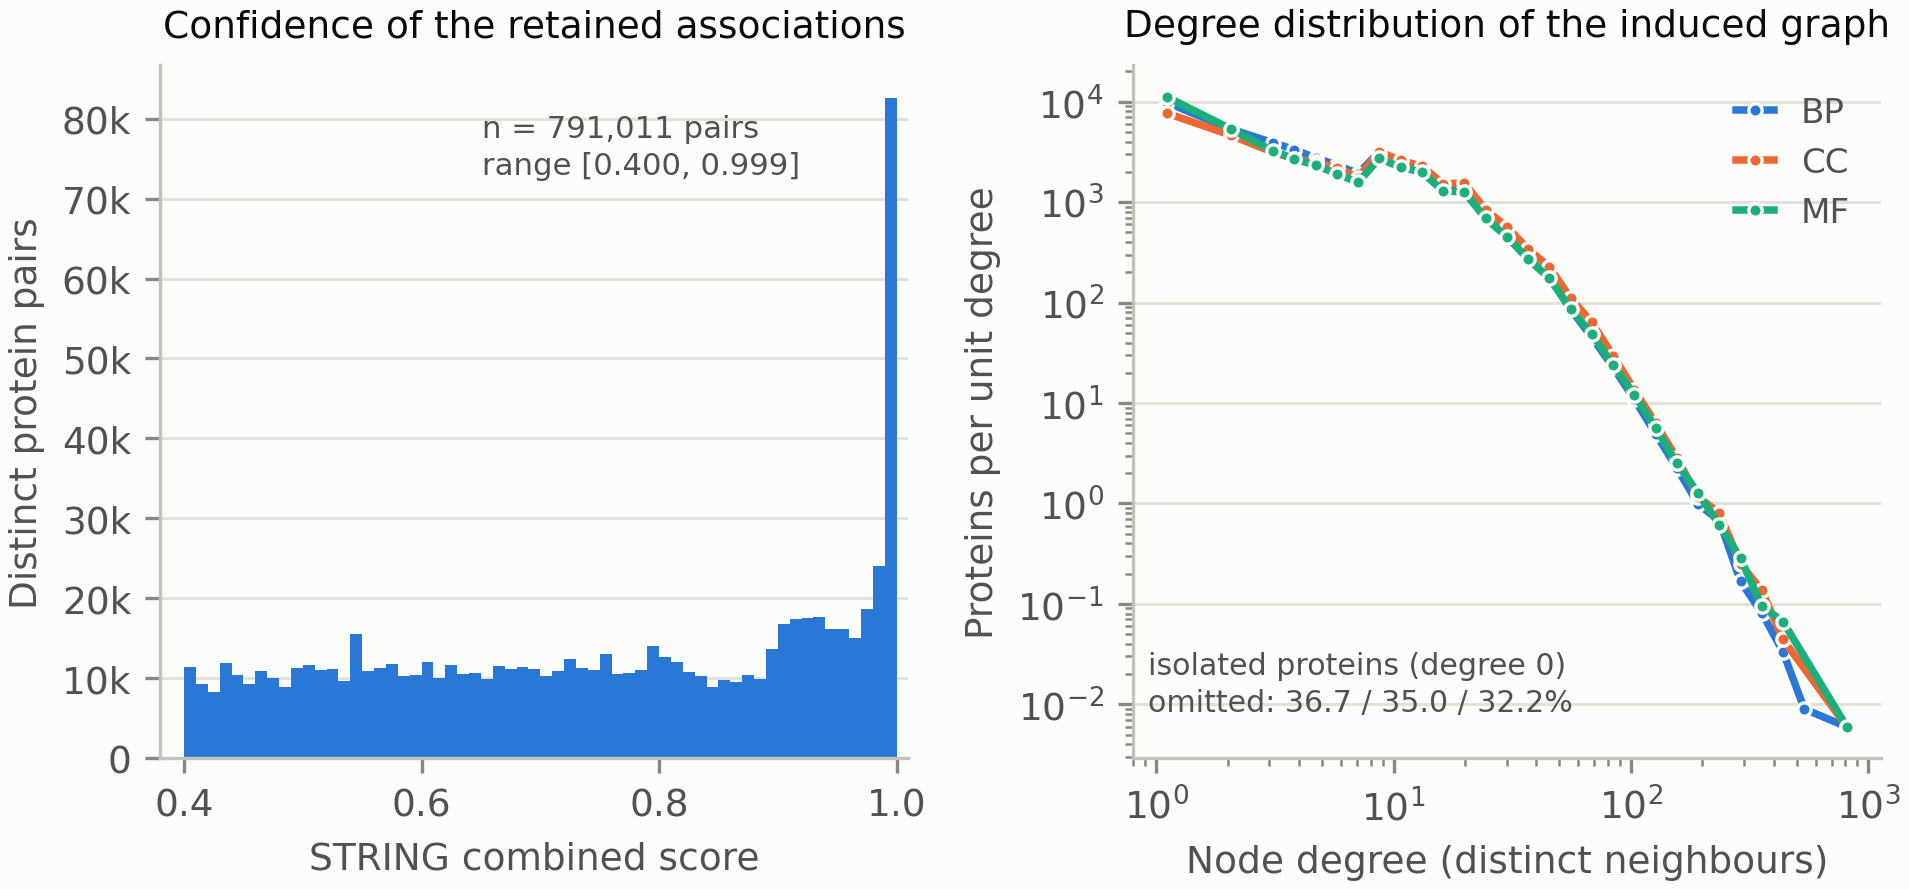
\includegraphics[width=\linewidth]{fig_cap4_score_and_degree.png}
    \caption{Left: distribution of the combined score over the $791{,}011$
    distinct protein pairs of the inherited file; since all records of a pair
    carry the same score, this distribution is independent of the deduplication
    strategy. Right: degree distribution of the three induced networks, in
    logarithmic scale; isolated proteins are omitted because the abscissa is
    logarithmic.}
    \label{fig:score_degree}
\end{figure}

Because the STRING combined score includes curated-database and text-mining channels, and because the corpus is not temporally separated from the network snapshot, some degree of knowledge circularity cannot be excluded. An association may indirectly reflect literature or curated biological knowledge related to the functions being predicted. The inherited file no longer preserves the channel-level provenance required to quantify or remove this effect. The graph-based gains should therefore be interpreted as gains obtained from the available aggregated STRING evidence, not as evidence that all graph information is independent of the target annotations.

\subsubsection{Composition of the Interaction Records}
\label{subsubsec:grafo_construcao}

The inherited file is a record-level rather than a pair-level listing. It
contains $2{,}422{,}234$ rows describing only $791{,}011$ distinct protein pairs
over $86{,}423$ distinct proteins, so that each pair is reported on average
$3.06$ times, and up to $170$ times. All rows referring to the same pair carry an identical score. The inherited file no longer contains sufficient provenance to determine whether the repetitions originated from distinct evidence channels or from another step in dataset assembly. They therefore do not provide independent confidence estimates.

Table~\ref{tab:multiplicidade} relates the number of rows of a pair to its
confidence. The mean combined score generally increases with the number of records, from $0.669$ for pairs described by a single row to $0.961$ for pairs described by $21$--$50$ rows, followed by a small decrease to $0.952$ for pairs with more than $50$ records; the rank correlation between the two quantities is $0.47$. Multiplicity is thus empirically concordant with
confidence without being determined by it. It should nonetheless not be read as
independent corroboration, since the combined score already aggregates the
evidence channels that produced the repeated rows: counting those rows again
re-weights evidence that the score has integrated once. What the multiplicity
provides is a second, coarser reading of the same evidence, and
Chapter~\ref{cap:metodologia} states the deduplication rule adopted and its
consequence for the distribution of edge weights.

\begin{table}[!htb]
    \centering
    \caption{Relationship between the number of evidence records reported for a
    protein pair and the mean combined score of the pairs in that group, over the $791{,}011$
    distinct pairs of the inherited file.}
    \label{tab:multiplicidade}
    \begin{tabular}{lrr}
    \toprule
    Records per Pair & Distinct Pairs & Mean Combined Score \\
    \midrule
    1        & 358,933 & 0.669 \\
    2        & 153,000 & 0.742 \\
    3        &  83,039 & 0.791 \\
    4--5     &  86,983 & 0.839 \\
    6--10    &  76,524 & 0.897 \\
    11--20   &  26,348 & 0.936 \\
    21--50   &   5,763 & 0.961 \\
    $>50$    &     421 & 0.952 \\
    \midrule
    Total    & 791,011 &       \\
    \bottomrule
    \end{tabular}
\end{table}

Converting this multi-record structure into an adjacency matrix requires an
explicit deduplication rule. Two strategies are evaluated: the maximum score
approach, which retains the highest single confidence value to keep weights within
the unit interval, and the summation approach, which accumulates scores to reflect
the volume of evidence. The formalization of these operators is detailed in
Chapter~\ref{cap:metodologia}.

\subsubsection{Topology of the Interaction Network}
\label{subsubsec:grafo_topologia}

The topological characteristics of the network (e.g., node counts, edge counts,
node degrees, and isolated proteins) depend strictly on edge existence.
Consequently, these metrics are invariant to the deduplication strategies discussed
above.

For each ontology, the network was induced over the union of the training,
validation, and test proteins, so that the node set coincides with the
corresponding row of Table~\ref{tab:cafa5}. Self-interactions were discarded and
each association was treated as undirected. Proteins without any retained
interaction were deliberately preserved as isolated nodes, so that the
ontology-specific populations remain unchanged and every protein is scored.

This decision affects graph connectivity, as quantified in
Figure~\ref{fig:iso_split}: approximately one third of the proteins in each
ontology have no mapped interaction ($33{,}797$ proteins or $36.65\%$ in BP,
$32{,}477$ or $34.95\%$ in CC, and $25{,}317$ or $32.19\%$ in MF). The
proportion is stable across the training, validation, and test subsets, which
indicates that the partition did not bias the topology of any subset. This is the
structural limitation that motivates the migration toward the multimodal
formulation of Chapter~\ref{cap:metodologia}: a method that represents a protein
exclusively by its interaction profile has, for one third of the corpus, no
information to operate on. Methods that restrict the feature basis to the
training proteins face a stricter version of the same limitation, since for them
a protein is uninformative unless it is connected to a training protein
specifically; that variant is quantified in Chapter~\ref{cap:metodologia}.

\begin{figure}[!htb]
    \centering
    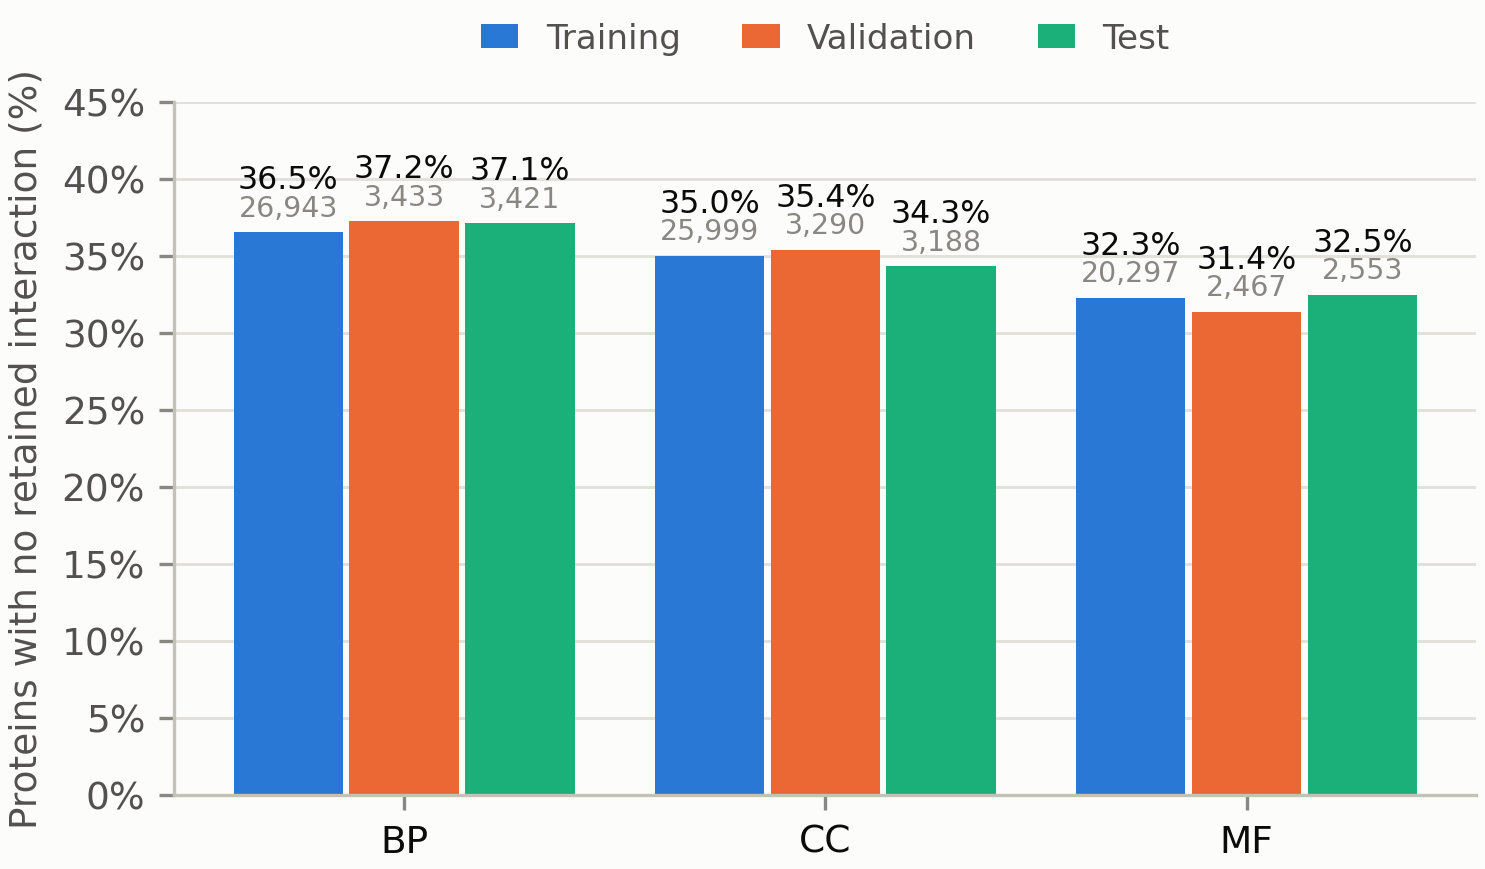
\includegraphics[width=0.82\linewidth]{fig_cap4_isolated_by_split.png}
    \caption{Proportion of proteins with no retained interaction, per ontology and
    per subset. Absolute counts are shown above each bar.}
    \label{fig:iso_split}
\end{figure}

Because the source data are pre-filtered for medium-confidence associations or
above, thresholding the graph within the $[0, 0.400]$ interval leaves the edge
set unchanged. As shown in Figure~\ref{fig:iso_thr}, the fraction of isolated
proteins remains constant up to $0.400$ and increases steeply thereafter,
exceeding half of the corpus at a $0.900$ threshold. Therefore, any threshold
at or below the data floor is inert, and the networks used herein coincide
with the complete inherited evidence.

\begin{figure}[!htb]
    \centering
    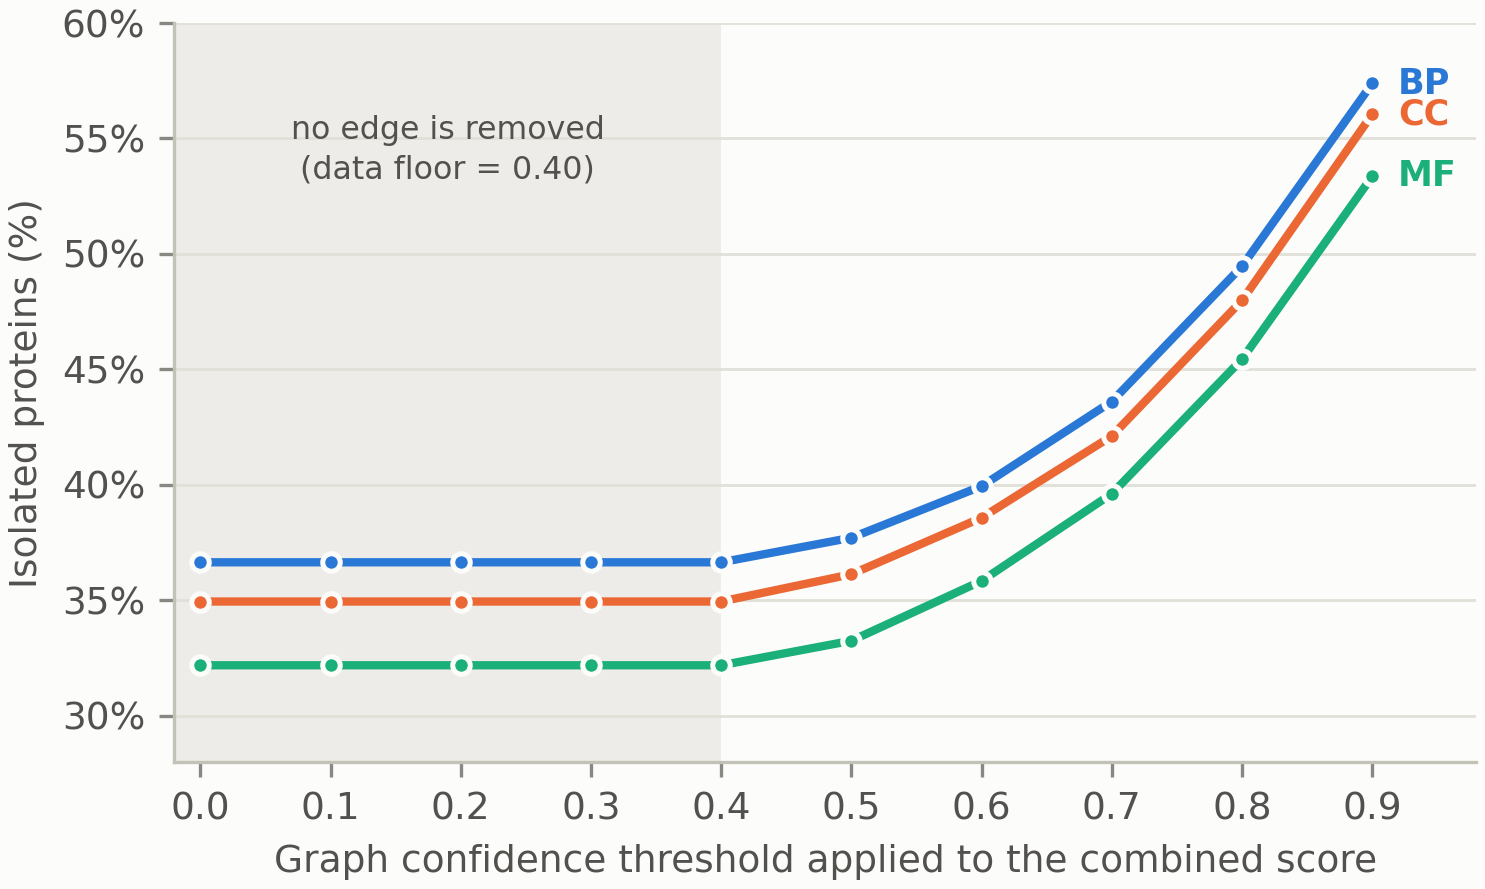
\includegraphics[width=0.82\linewidth]{fig_cap4_isolated_vs_threshold.png}
    \caption{Fraction of isolated proteins as a function of the confidence
    threshold applied to the combined score. The shaded region marks the interval
    in which no edge is removed, since the source data are floored at $0.400$.}
    \label{fig:iso_thr}
\end{figure}

Table~\ref{tab:grafo} summarizes the topology of the three induced networks. Node
degree is reported as the number of distinct neighbors of a protein, and should
not be confused with the number of evidence records incident to it, which is
larger by a factor of approximately three and which is relevant only to the
weighting strategies of Chapter~\ref{cap:metodologia}.

\begin{table}[!htb]
    \centering
    \caption{Topology of the ontology-specific interaction networks, induced over
    the union of the training, validation, and test proteins. Degree denotes the
    number of distinct neighbors, so that the reported values do not depend on
    the deduplication strategy adopted for the edge weights.}
    \label{tab:grafo}
    \begin{tabular}{lrrr}
    \toprule
    Statistic & BP & CC & MF \\
    \midrule
    Nodes                              & 92,210  & 92,912  & 78,637  \\
    Undirected edges                   & 492,920 & 566,566 & 470,206 \\
    Isolated proteins                  & 33,797  & 32,477  & 25,317  \\
    Isolated proteins (\%)             & 36.65   & 34.95   & 32.19   \\
    \midrule
    \multicolumn{4}{l}{\emph{Node degree}} \\
    \quad Mean                         & 10.7    & 12.2    & 12.0    \\
    \quad Median                       & 5       & 7       & 7       \\
    \quad Standard deviation           & 17.4    & 19.0    & 19.1    \\
    \quad Minimum                      & 0       & 0       & 0       \\
    \quad 1st quartile                 & 0       & 0       & 0       \\
    \quad 3rd quartile                 & 15      & 17      & 16      \\
    \quad Maximum                      & 763     & 798     & 805     \\
    \bottomrule
    \end{tabular}
\end{table}

The degree distributions are strongly right-skewed in the three ontologies: the
mean exceeds the median, the first quartile is zero, and the maximum degree is
roughly fifty times the third quartile. The networks thus combine a large
population of isolated or weakly connected proteins with a small set of densely
connected ones, a shape that Figure~\ref{fig:score_degree} (right) shows to span approximately
two orders of magnitude and to be essentially identical across the three ontologies. High degree does not strictly imply biological
centrality, as it also reflects unequal experimental coverage and the availability
of evidence channels favoring well-studied proteins~\cite{barabasi2004network}.
This topological heterogeneity constrains the propagation mechanisms: aggregation
schemes must remain informative for isolated nodes while avoiding domination by
large neighborhoods. The mechanisms addressing these requirements are presented
in Chapter~\ref{cap:metodologia}.

\section{Evaluation Protocol}
\label{sec:protocolo}

This section establishes the universe boundaries and processing conventions required
prior to metric computation. These structural choices apply uniformly to all metrics
and models.

\paragraph{Evaluation universe.}
All metrics are computed independently for each ontology $d \in \{\mathrm{BP},
\mathrm{MF}, \mathrm{CC}\}$, restricted to the retained term vocabulary
$\mathcal{C}_d$ introduced in Section~\ref{subsec:rotulos}, and never over the
complete Gene Ontology. For a protein $i$, let $T_i \subseteq \mathcal{C}_d$
denote its set of ground-truth annotations within that vocabulary, and let $n$
denote the number of proteins in the subset being evaluated. Terms lying
outside $\mathcal{C}_d$ are neither predicted nor scored, and consequently
neither contribute to nor penalize any of the reported values. Comparisons with
externally published values must therefore account for discrepancies in the
scored vocabularies, since identical formulas yield different numerical results
over distinct term sets.

\paragraph{Hierarchical consistency of the annotations.}
The ground-truth annotation sets inherited with the dataset are already closed
under the ancestor relation: for every protein and every annotated term, all
ancestors of that term belonging to $\mathcal{C}_d$ are annotated as well, both
through the \texttt{is\_a} and through the \texttt{part\_of} relation. No
propagation is therefore applied to the labels at any stage, neither during
training nor during evaluation.

\paragraph{Hierarchical consistency of the predictions.}
Model outputs, in contrast, are not guaranteed to respect the ontology. A model
may assign a high score to a specific term and a low score to one of its
ancestors, which is semantically inconsistent. Before any metric is computed, the
predicted scores are therefore made hierarchy-consistent by raising the score of
each term to the maximum score observed over that term and its descendants,
\begin{equation}
\label{eq:prop_pred}
\tilde{s}_{iv} \;=\; \max_{u \,\in\, \mathcal{D}(v)} s_{iu},
\qquad
\mathcal{D}(v) \;=\; \{v\} \,\cup\,
\bigl\{\, u \in \mathcal{C}_d \;:\; v \in \mathrm{anc}(u) \,\bigr\},
\end{equation}
\noindent where $s_{iu}$ is the raw score assigned by the model to term $u$ for protein
$i$, and $\mathrm{anc}(u)$ is the ancestor closure of $u$ within $\mathcal{C}_d$.
The set $\mathcal{D}(v)$ contains $v$ itself, so the operation is well defined
for terms that have no descendant in $\mathcal{C}_d$, and it can only raise a
score, never lower one. This operation is applied uniformly to every model and to
every reimplemented baseline, and it is applied exclusively to predictions, never
to features or to labels.

The ancestor closure $\mathrm{anc}(\cdot)$ used in Equation~\ref{eq:prop_pred}
traverses only the \texttt{is\_a} relation, following the convention established
for the evaluation of ontology-aware predictors~\cite{kulmanov2018deepgo}.
Ancestors reachable exclusively through \texttt{part\_of} therefore do not
receive the score of their descendants. The extent of this restriction varies
across ontologies: it affects $387$ of the $3{,}507$ ancestor-descendant pairs in
BP ($11.0\%$), $2{,}056$ of $4{,}405$ in CC ($46.7\%$), and a single pair in MF.
The restriction affects all methods identically at the post-processing level, but the direction of its effect on the metrics is not guaranteed: propagating additional \texttt{part\_of} relations could increase both true-positive and false-positive scores. The reported values therefore correspond specifically to the \texttt{is\_a}-only prediction-closure convention, which differs from the \texttt{is\_a}-plus-\texttt{part\_of} closure already present in the ground truth and is particularly consequential for Cellular Component.


\paragraph{Decision thresholds.}
Threshold-swept metrics require an explicit grid, since the reported maxima and
minima are taken over it. All such metrics are evaluated over
\begin{equation}
\label{eq:limiares}
\mathcal{T} = \{0.00,\ 0.01,\ 0.02,\ \ldots,\ 1.00\},
\end{equation}
\noindent that is, $101$ evenly spaced thresholds spanning the full range of the predicted
probabilities. For each $\tau \in \mathcal{T}$, the predicted term set of protein
$i$ is
\begin{equation}
\label{eq:conjunto_predito}
P_i(\tau) = \bigl\{\, v \in \mathcal{C}_d \;:\; \tilde{s}_{iv} \geq \tau \,\bigr\},
\end{equation}
\noindent built from the hierarchy-consistent scores of Equation~\ref{eq:prop_pred}.

\paragraph{Averaging conventions.}
All metrics adopted in this work are protein-centric: a value is computed for
each protein and subsequently averaged over the evaluated subset. Two distinct
denominators are used. Precision is averaged only over the proteins that received
at least one predicted term at the threshold under consideration, whose number is
denoted by
\begin{equation}
\label{eq:m_tau}
m(\tau) = \bigl| \{\, i \;:\; P_i(\tau) \neq \varnothing \,\} \bigr|,
\end{equation}
\noindent whereas recall is averaged over all $n$ proteins of the subset, including those
for which nothing was predicted. This corresponds to the full evaluation mode of
the CAFA assessments, under which a protein that receives no prediction
contributes zero recall rather than being excluded. When no protein receives any
prediction, that is, when $m(\tau) = 0$, precision is defined as zero.

\paragraph{Model selection and test reporting.}
Two distinct criteria operate at two distinct levels, and they are separated
deliberately. Within a single training run, the epoch retained for evaluation is
the one that minimizes the loss on the validation subset, as specified in
Section~\ref{sec:met_selecao}. Across runs, $wF_{\max}$
(Section~\ref{subsec:wfmax}) is the criterion that selects between
configurations: architectures, hyperparameters, and combination coefficients were
compared exclusively on the validation subset. The selected configuration was then
frozen and evaluated once on the test subset, so that no test annotation informed
any development decision. The test values reported in
Chapter~\ref{cap:resultados} therefore represent a single evaluation of a fixed
configuration, rather than an empirical maximum.

\section{Evaluation Metrics}
\label{sec:metricas}

Model performance was assessed using six protein-centric metrics, presented below
and reported throughout this dissertation in a single order: the maximum
F-measure $F_{\max}$, its root-excluded variant $F_{\max}^{*}$, its weighted
counterpart $wF_{\max}$, the minimum semantic distance $S_{\min}$, and the two
areas under the precision-recall curve, AuPRC and IAuPRC. The measures
$F_{\max}$, $wF_{\max}$ and $S_{\min}$ follow the threshold-swept and semantic
evaluation adopted in the CAFA assessments~\cite{radivojac2013large,
zhou_cafa_2019}. The root-excluded variant and the area under the
precision-recall curve are complementary measures, and the interpolated area is
adopted from previous work of this research group~\cite{oliveira2025supermagov2}.
All six are computed over the evaluation universe, the hierarchy-consistent
scores, and the threshold grid established in Section~\ref{sec:protocolo}.

\subsection{Information Content}
\label{subsec:ic}

Terms of the Gene Ontology differ both in semantic specificity and in empirical
frequency. Terms close to the root of an ontology are usually broad and
frequently annotated, whereas their more specific descendants tend to occur less
often. Ontology depth and dataset frequency are not strictly equivalent: a deep
term may be common, while a shallow term may be rare within a specific corpus.
The semantic weight used by the metrics below is therefore estimated from
annotation frequencies rather than from depth.

The quantity adopted is the information content of a term, which measures the
information a term contributes beyond what its parents already convey. For
a term $v$ with direct parents $\mathrm{pa}(v)$, it is defined as
\begin{equation}
\label{eq:ic}
\mathrm{IC}(v) = -\log_{2} \widehat{P}\bigl(v \mid \mathrm{pa}(v)\bigr),
\end{equation}
\noindent where $\widehat{P}(v \mid \mathrm{pa}(v))$ is the proportion of annotated
proteins carrying $v$ among those carrying all of its parent terms. A term that
follows almost deterministically from its parents therefore receives a weight
close to zero, whereas a term that is rarely observed given its parents receives
a high weight. The root of each ontology, being annotated for every protein,
receives $\mathrm{IC} = 0$ and consequently contributes nothing to any weighted
metric, which is the formal counterpart of the observation made in
Section~\ref{subsec:rotulos}.

The conditional proportions of Equation~\ref{eq:ic} are estimated on the training
subset alone, so that the weighting is fixed before any validation or test
protein is scored. The resulting information content vector is inherited with the
consolidated dataset and kept unchanged across the three subsets. Its magnitude
varies markedly between ontologies: the median weight is $1.06$ bits in BP,
$2.05$ in CC, and $1.50$ in MF, with maxima of $5.54$, $9.79$, and $9.26$ bits,
respectively. Weighted metrics computed in different ontologies are therefore not
directly comparable to one another.

\subsection{Maximum F-measure (\texorpdfstring{$F_{\max}$}{Fmax})}
\label{subsec:fmax}

For a given threshold $\tau \in \mathcal{T}$, the protein-centric precision and
recall are obtained by averaging the per-protein proportions of correctly
predicted terms, following the denominators established in
Section~\ref{sec:protocolo}:
\begin{equation}
\label{eq:pr_rc}
pr(\tau) = \frac{1}{m(\tau)}
\sum_{i \,:\, P_i(\tau) \neq \varnothing}
\frac{\bigl| P_i(\tau) \cap T_i \bigr|}{\bigl| P_i(\tau) \bigr|},
\qquad
rc(\tau) = \frac{1}{n}
\sum_{i=1}^{n}
\frac{\bigl| P_i(\tau) \cap T_i \bigr|}{\bigl| T_i \bigr|}.
\end{equation}

The maximum F-measure is the highest harmonic mean of these two quantities over
the threshold grid:
\begin{equation}
\label{eq:fmax}
F_{\max} = \max_{\tau \in \mathcal{T}}
\left\{
\frac{2 \cdot pr(\tau) \cdot rc(\tau)}{pr(\tau) + rc(\tau)}
\right\}.
\end{equation}

\subsection{Root-Excluded Maximum F-measure (\texorpdfstring{$F_{\max}^{*}$}{Fmax*})}
\label{subsec:fmaxstar}

The variant tabulated as $F_{\max}^{*}$ applies Equations~\ref{eq:pr_rc}
and~\ref{eq:fmax} unchanged, after removing the root term of the corresponding
ontology from every ground-truth and predicted term set. As established in
Section~\ref{subsec:rotulos}, the root is a positive label for every protein in
the corpus, so a model that predicts it confidently obtains a correct prediction
at no cost. Excluding it prevents this trivially satisfiable term from
contributing to precision and recall, and yields a stricter reading of the same
quantity.

The removal admits a degenerate case that requires an explicit convention. Since
the ground-truth sets are closed under the ancestor relation, a protein annotated
with a single term is annotated with the root alone, and its ground-truth set
becomes empty once the root is removed; Table~\ref{tab:rotulos} shows that such
proteins exist in BP and MF. A protein in this situation contributes zero recall
and remains in the denominator $n$ of Equation~\ref{eq:pr_rc}, consistent with
the full evaluation mode of Section~\ref{sec:protocolo}. The restriction of the
label space therefore cannot raise $F_{\max}^{*}$ by silently discarding the
proteins it makes hardest to score. Symmetrically, a protein whose predicted set
becomes empty after the removal is excluded from the precision average, exactly
as in $m(\tau)$.

This metric remains protein-centric: it aggregates per-protein proportions
exactly as $F_{\max}$ does, and differs from it solely by the removal of one
term. It should not be confused with a term-centric evaluation, which would fix a
term and assess its performance across proteins.

\subsection{Maximum Weighted F-measure (\texorpdfstring{$wF_{\max}$}{wFmax})}
\label{subsec:wfmax}

$wF_{\max}$ was adopted as the criterion for selecting between configurations in
this work. It replaces the term counts of Equation~\ref{eq:pr_rc} with sums of
information-content weights, so that both correct and incorrect predictions
involving informative terms carry more influence than predictions involving
highly frequent ones:
\begin{equation}
\label{eq:wpr}
wpr(\tau) = \frac{1}{m_w(\tau)}
\sum_{i \,:\, \mathrm{IC}(P_i(\tau)) > 0}
\frac{\sum_{v \in P_i(\tau) \cap T_i} \mathrm{IC}(v)}
     {\sum_{v \in P_i(\tau)} \mathrm{IC}(v)},
\end{equation}
\begin{equation}
\label{eq:wrc}
wrc(\tau) = \frac{1}{n} \sum_{i \,:\, \mathrm{IC}(T_i) > 0}
\frac{\sum_{v \in P_i(\tau) \cap T_i} \mathrm{IC}(v)}
     {\sum_{v \in T_i} \mathrm{IC}(v)},
\end{equation}
\noindent where $\mathrm{IC}(P_i(\tau)) = \sum_{v \in P_i(\tau)} \mathrm{IC}(v)$ denotes
the total weight of the predicted set, $\mathrm{IC}(T_i)$ is defined analogously
over the ground-truth set, and $m_w(\tau)$ is the number of proteins for which
the former is strictly positive. This denominator differs from $m(\tau)$ only in
the degenerate case of a protein whose entire prediction carries null weight.

Equation~\ref{eq:wrc} requires a convention of its own, since the weight of a
ground-truth set may also vanish. As the root carries $\mathrm{IC} = 0$, this is
the situation of a protein annotated with the root alone, that is, the same
population identified in Section~\ref{subsec:fmaxstar}. Such a protein
contributes nothing to the summation and nevertheless remains in the denominator
$n$, exactly as an unpredicted protein does in Equation~\ref{eq:pr_rc}: a protein
about which the retained vocabulary asserts nothing informative cannot be
recalled informatively, and it is not removed from the evaluated population on
that account. The metric is then
\begin{equation}
\label{eq:wfmax}
wF_{\max} = \max_{\tau \in \mathcal{T}}
\left\{
\frac{2 \cdot wpr(\tau) \cdot wrc(\tau)}{wpr(\tau) + wrc(\tau)}
\right\}.
\end{equation}

Because the maximizing threshold is located using the annotations of the subset
being evaluated, $wF_{\max}$ is a threshold-swept summary of the score ranking
rather than the performance of a threshold fixed in advance. The comparisons of
Chapter~\ref{cap:resultados} are consistent in this respect, since the same
convention is applied to every method.

\subsection{Minimum Semantic Distance (\texorpdfstring{$S_{\min}$}{Smin})}
\label{subsec:smin}

Whereas the F-measures reward agreement, $S_{\min}$ quantifies the semantic cost
of disagreement, weighting each error by the information content of the term
involved~\cite{radivojac2013large}. Two complementary costs are accumulated.
Remaining uncertainty is the average weight of the true terms the model failed to
predict,
\begin{equation}
\label{eq:ru}
\mathrm{RU}(\tau) = \frac{1}{n} \sum_{i=1}^{n}
\sum_{v \in T_i \setminus P_i(\tau)} \mathrm{IC}(v),
\end{equation}
\noindent and misinformation is the average weight of the terms the model incorrectly
activated,
\begin{equation}
\label{eq:mi}
\mathrm{MI}(\tau) = \frac{1}{n} \sum_{i=1}^{n}
\sum_{v \in P_i(\tau) \setminus T_i} \mathrm{IC}(v).
\end{equation}

At each threshold these two costs define a point in the $(\mathrm{RU},
\mathrm{MI})$ plane, and the semantic distance is their Euclidean combination.
The metric is the minimum of that distance over the threshold grid:
\begin{equation}
\label{eq:smin}
S_{\min} = \min_{\tau \in \mathcal{T}}
\sqrt{\mathrm{RU}(\tau)^{2} + \mathrm{MI}(\tau)^{2}}.
\end{equation}

Unlike the F-measures, $S_{\min}$ is expressed in bits and is to be minimized.

\subsection{Area Under the Precision-Recall Curve}
\label{subsec:auprc}

The pairs $\bigl(rc(\tau), pr(\tau)\bigr)$ obtained across the threshold grid
trace a precision-recall curve, whose area summarizes the quality of the score
ranking without committing to any particular threshold. This curve is constructed
from the unweighted precision and recall (Equation~\ref{eq:pr_rc}), rather than
their information-content-weighted counterparts.

Let $(r_k, p_k)$, for $k = 1, \ldots, K$ with $K = |\mathcal{T}|$, denote the
curve points reordered so that $0 \leq r_1 \leq r_2 \leq \cdots \leq r_K \leq 1$.
The area is computed by the trapezoidal rule,
\begin{equation}
\label{eq:auprc}
\mathrm{AuPRC} = \sum_{k=1}^{K-1} \bigl(r_{k+1} - r_k\bigr)
\cdot \frac{p_k + p_{k+1}}{2},
\end{equation}
\noindent which interpolates linearly between consecutive observed operating points. The
curve is not anchored at recall $0$ or at recall $1$, so the rule integrates only
over the recall interval spanned by the observed operating points.

\subsection{Interpolated Area Under the Precision-Recall Curve}
\label{subsec:iauprc}

Empirical precision-recall curves are not monotone: precision may decrease and
then recover as the threshold is relaxed. The interpolated variant replaces the
observed precision by its monotone envelope, evaluated on a grid of recall levels
rather than on the threshold grid of Equation~\ref{eq:limiares}. Let
\begin{equation}
\label{eq:grade_recall}
\mathcal{R} = \{0.00,\ 0.01,\ 0.02,\ \ldots,\ 1.00\}
\end{equation}
\noindent denote that grid, numerically identical to $\mathcal{T}$ but indexing recall
rather than score. For each level $\rho \in \mathcal{R}$ that does not exceed the
maximum recall attained by the model, the interpolated precision is the best
precision observed at that level or beyond,
\begin{equation}
\label{eq:iauprc}
p_{\mathrm{interp}}(\rho) = \max_{k \,:\, r_k \geq \rho} p_k.
\end{equation}

Denoting by $\rho_1 < \rho_2 < \cdots < \rho_L$ the levels of $\mathcal{R}$ that
satisfy this condition, the area under the resulting envelope is obtained with the
integration rule of Equation~\ref{eq:auprc},
\begin{equation}
\label{eq:iauprc_area}
\mathrm{IAuPRC} = \sum_{\ell=1}^{L-1} \bigl(\rho_{\ell+1} - \rho_{\ell}\bigr)
\cdot \frac{p_{\mathrm{interp}}(\rho_{\ell}) + p_{\mathrm{interp}}(\rho_{\ell+1})}{2}.
\end{equation}

Recall levels above the maximum attained by the model are discarded rather than
extrapolated, so the integration stops at that point. The envelope reports, for
each recall level, the best precision the model reaches at that level or beyond;
IAuPRC therefore characterizes the achievable operating points of the score
ranking, and complements AuPRC, which follows the empirical curve point by point.

\section{Direction, Scale and Variability of the Reported Values}
\label{sec:escala}

The defined metrics vary in range and direction of improvement. The measures
$F_{\max}$, $F_{\max}^{*}$, $wF_{\max}$, AuPRC and IAuPRC are bounded in $[0, 1]$
and are to be maximized. $S_{\min}$ is non-negative, has no upper bound, is
expressed in bits, and is to be minimized. In the ablation and model-selection
tables of Chapter~\ref{cap:resultados}, the bounded metrics are multiplied by $100$
and reported as percentages; $S_{\min}$ is reported in its original scale.

Unless explicitly stated otherwise, every reported value represents a point
estimate from a single partition and random seed, precluding confidence intervals.
Consequently, minor numerical variations do not reliably indicate model superiority.
The analysis conducted in Chapter~\ref{cap:resultados} accordingly emphasizes
differences that persist consistently across ontologies and across metrics, rather
than isolated marginal improvements in a single cell.




% =====================================================================
% CAPÍTULO 5 — PROPOSED METHODOLOGY   (versão v4)
% =====================================================================

\chapter{Proposed Methodology}
\label{cap:metodologia}

\section{Overview}
\label{sec:met_overview}

The task addressed in this dissertation is multi-label classification over a fixed vocabulary of
approximately five hundred Gene Ontology terms per ontology, formulated as node classification
on a graph whose vertices are proteins and whose edges are protein-protein
interactions reported by STRING. The corpus, the partitions, the hierarchical closure of the
ground-truth annotations, and the six evaluation metrics were established in
Chapter~\ref{cap:materiais}; this chapter specifies the models that consume that material.

The methodology developed here evolved in two generations. The first generation investigates
how much of a protein's function can be recovered exclusively from its position in the STRING
network. It represents each protein by its interaction profile, with no sequence
information, and explores several ways of mapping that profile to a prediction. This
approach is bounded by a structural limitation inherent to the network coverage. The second
generation addresses this limitation by introducing a sequence representation derived from a
protein language model and treating the network as a mechanism for propagating that
representation among interacting proteins.

The framework that results from the second generation is referred to as NEXUS-GO
(Network-Extended Unified Sequence Embeddings for Gene Ontology function annotation). It admits
four routes, named here for later reference: NEXUS-GO/Fixed, which propagates the sequence
representation over the network without learning the aggregation (Section~\ref{sec:met_fixa});
NEXUS-GO/GNN, which applies a graph encoder trained end to end (Section~\ref{sec:met_gnn}); and NEXUS-GO/Early and
NEXUS-GO/Late, which combine the two at the representation and at the prediction level
(Sections~\ref{sec:met_early} and~\ref{sec:met_late}). The first generation, which consumes no
sequence information, is reported throughout as a topology-only control and carries no name.

Within each generation, every model decomposes into the same three independent decisions, and this
decomposition organizes Sections~\ref{sec:met_gen1} and~\ref{sec:met_repr}, each of which is structured around these three core components:
\begin{itemize}
  \item \textbf{Representation}: the input vector of a protein;
  \item \textbf{Propagation}: the mechanism by which the neighborhood modifies the representation;
  \item \textbf{Prediction head}: the transformation of the resulting vector into per-term scores.
\end{itemize}

Figure~\ref{fig:met_chapter_map} places the two generations against this axis and marks the
limitation that separates them.

\begin{figure}[!htb]
  \centering
  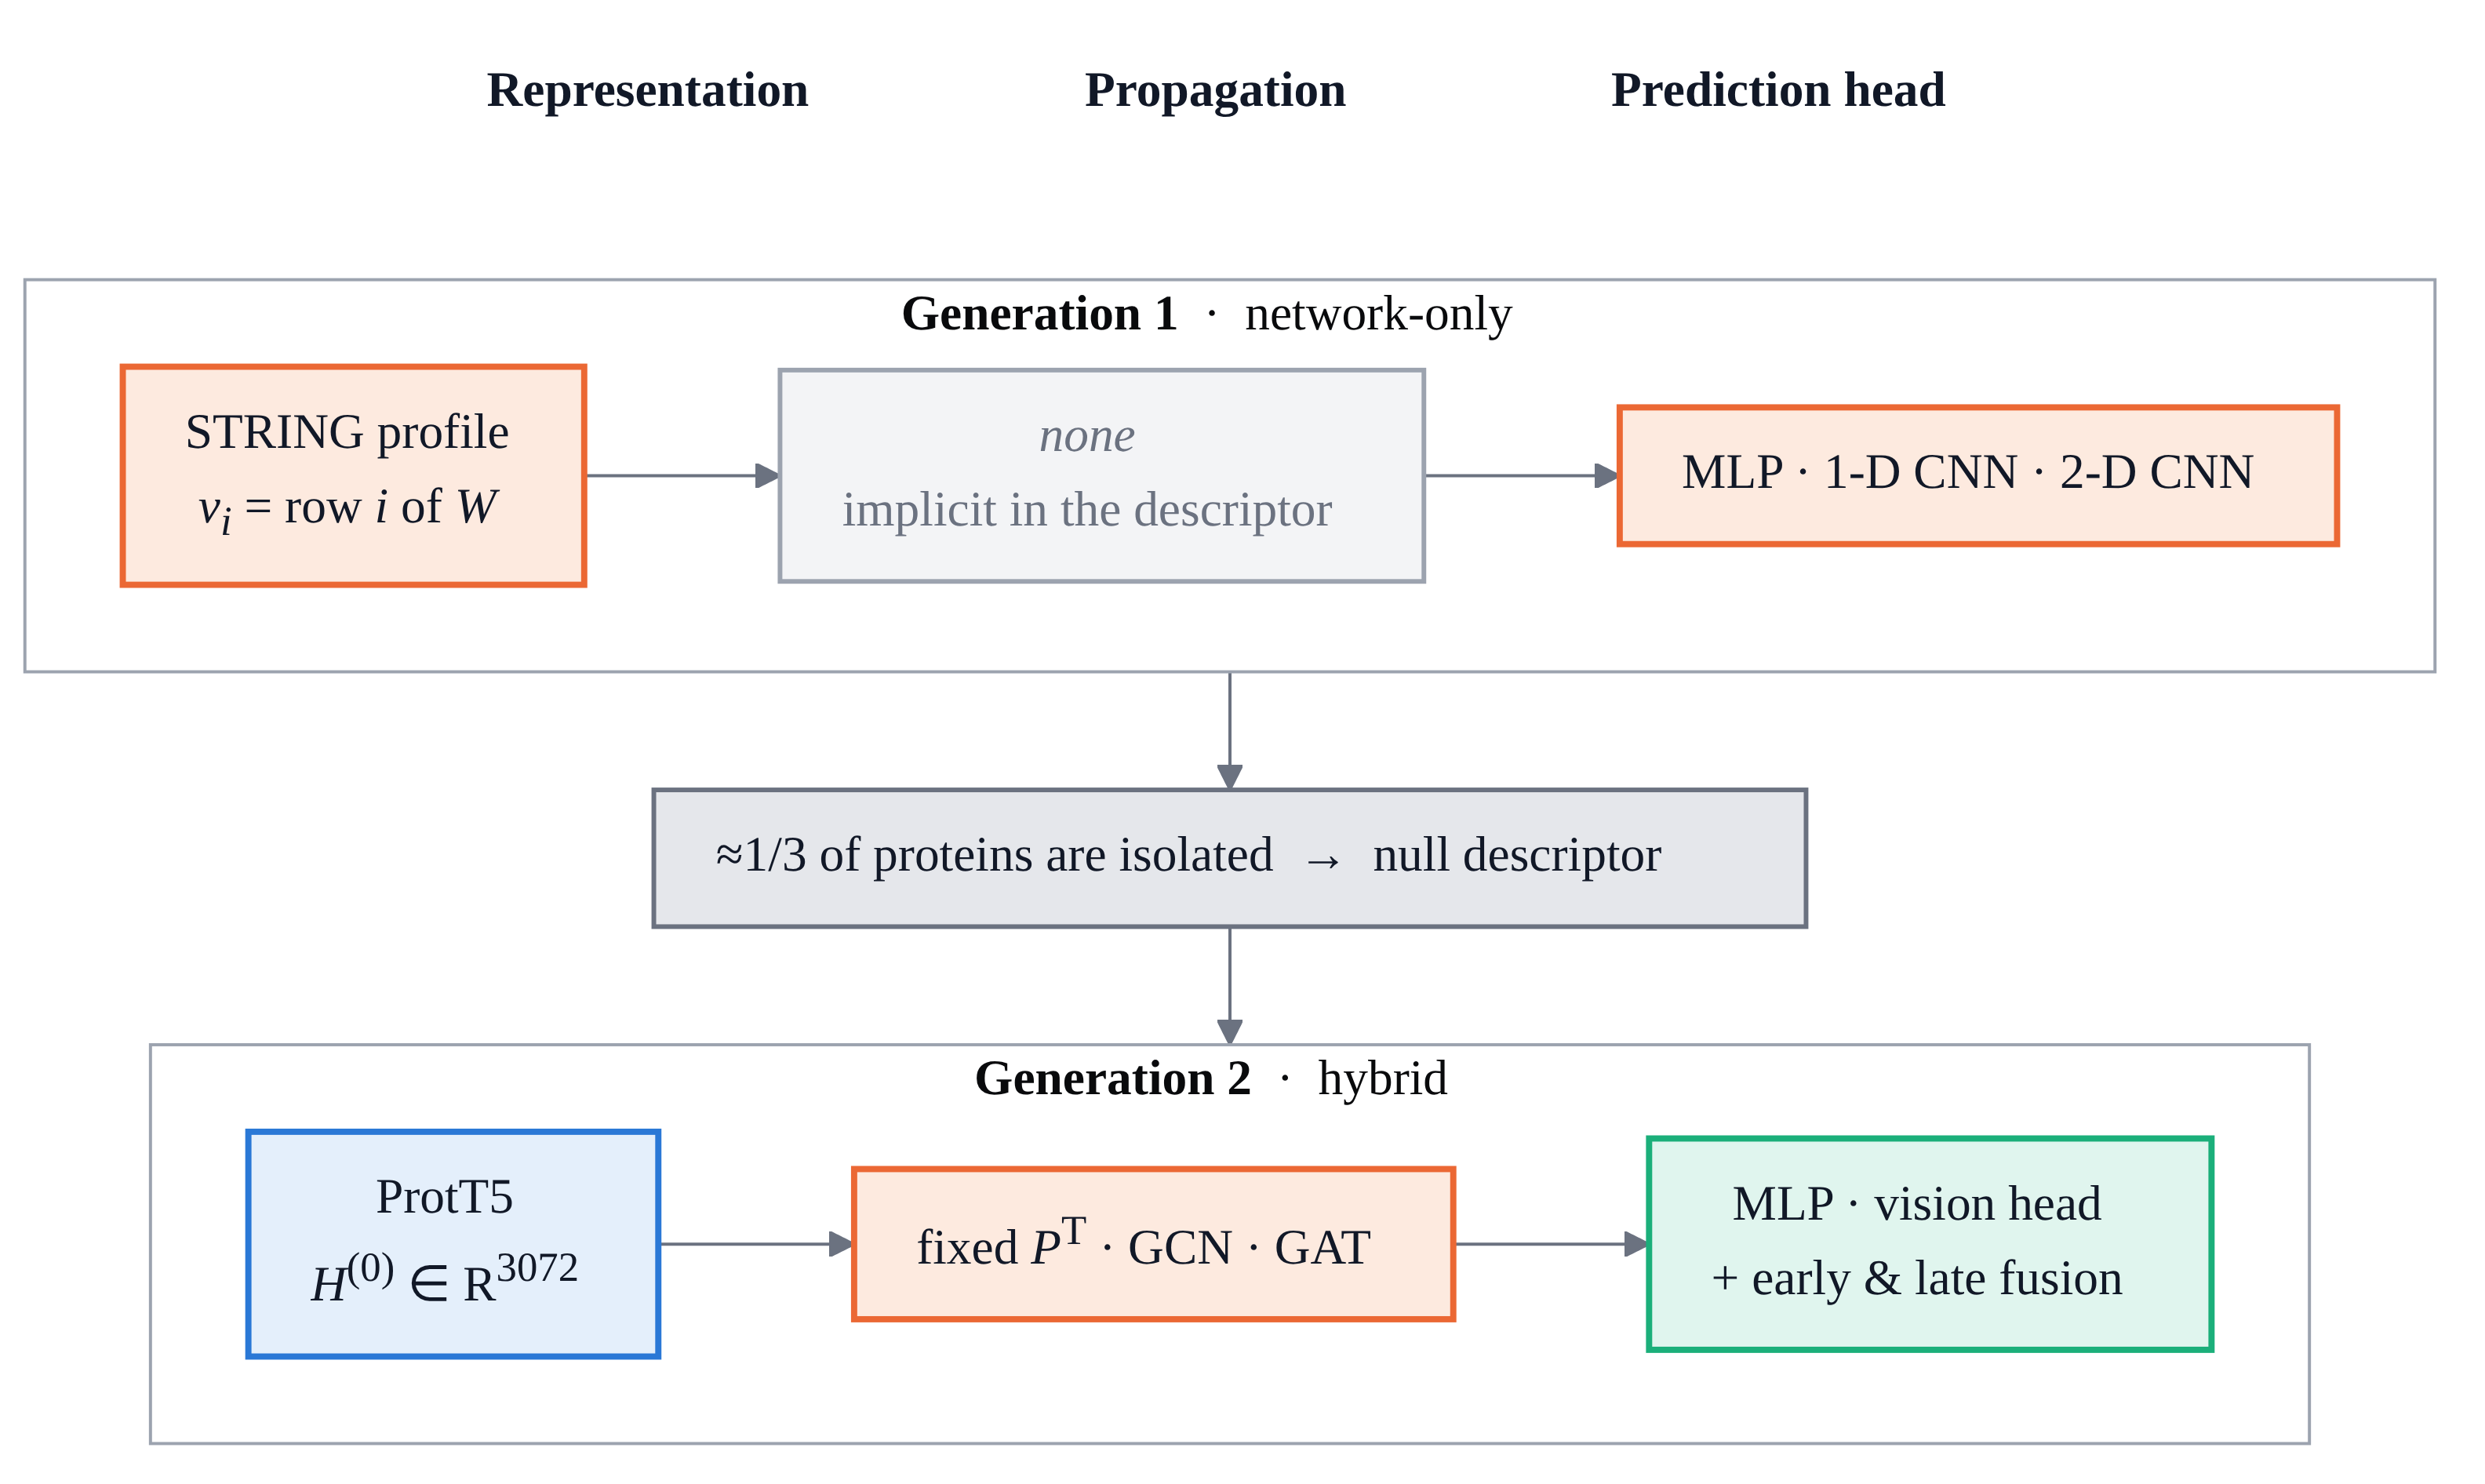
\includegraphics[width=\textwidth]{cap5/fig_5_01_chapter_map.png}
  \caption[Map of the proposed methodology]{Map of the proposed methodology. The two generations
  (rows) are crossed with the methodological axis Representation $\rightarrow$ Propagation
  $\rightarrow$ Prediction head (columns). The band between the rows states the limitation of the
  first generation that motivates the second.}
  \label{fig:met_chapter_map}
\end{figure}

\paragraph{Notation.} Throughout the chapter, $\mathbf{H}^{(h)}$ denotes the matrix of node
representations after $h$ propagation steps, where $h = 0, 1, \dots, T$ and $T$ is the total number
of steps; $\mathbf{H}^{(0)}$ is the node attribute matrix defined in Equation~\eqref{eq:met_h0}.
Boldface uppercase symbols denote matrices, boldface lowercase symbols denote vectors, and
lightface symbols denote scalars. The symbol $\alpha$ is reserved for the mixing coefficient of the
fixed propagation operator; the attention coefficients of Section~\ref{sec:met_gnn} are written
$a_{ij}$, the linear mixing coefficient of Section~\ref{sec:met_late} is written $\gamma$, and the
blending coefficient of Equation~\eqref{eq:met_ens_w} is written $\lambda$. Trainable weight
matrices are written $\Theta$, and $W$ is reserved for the weighted adjacency matrix of the
interaction graph.

% =====================================================================
\section{Learning Regime and Supervision Masking}
\label{sec:met_regime}

The evaluation protocol (the corpus partitions, the hierarchical closure of the ground-truth
annotations, and the six metrics) is defined in Chapter~\ref{cap:materiais} and is shared by the
proposed models and the comparative methods. This section specifies the data each model is allowed
to observe during training. A protein belonging to the validation or test partition is a vertex
of the same graph as the training proteins, which makes an explicit partition boundary necessary.

\subsection{Transductive Node Classification}
\label{sec:met_transdutivo}

The interaction graph is assembled once over the union of the three partitions,
\begin{equation}
  \mathcal{V} \;=\; \mathcal{V}_{\text{train}} \,\cup\, \mathcal{V}_{\text{val}} \,\cup\, \mathcal{V}_{\text{test}},
  \label{eq:met_universo}
\end{equation}
\noindent so that the vertex set contains $92{,}210$ proteins for Biological Process, $92{,}912$ for Cellular
Component, and $78{,}637$ for Molecular Function. Validation and test proteins are present in the
graph as carriers of node attributes and edges, but never as carriers of labels. The
models are therefore transductive in the sense established for semi-supervised learning on graphs:
the unlabeled portion of the vertex set is visible at training time, but only through its features
and its connectivity~\cite{yang2016revisiting}.

Supervision is restricted by masking. Let $\mathrm{loss}(\cdot,\cdot)$ denote the per-protein loss and
$\hat{\mathbf{y}}_i$ the prediction for protein $i$; the quantity that is minimized is
\begin{equation}
  \mathcal{L} \;=\; \frac{1}{|\mathcal{V}_{\text{train}}|}
  \sum_{i \,\in\, \mathcal{V}_{\text{train}}} \mathrm{loss}\!\left(\hat{\mathbf{y}}_i,\; \mathbf{y}_i\right),
  \label{eq:met_mascara}
\end{equation}
\noindent where $\hat{\mathbf{y}}_i$ may depend on the whole graph, but $\mathbf{y}_i$ is read only for
$i \in \mathcal{V}_{\text{train}}$. Operationally, the sampler that feeds the optimizer emits
training indices only, so no gradient is ever computed against an annotation outside the training
partition. No label of a validation or test protein is read during optimization; what crosses the
partition boundary is topology and node attributes, both of which are observable at prediction time
and neither of which encodes the target.

Sharing structure is the defining assumption of transductive learning; the graph is a single object,
and removing part of it at training time would alter the modeled topology. Sharing labels constitutes
leakage, which Equation~\eqref{eq:met_mascara} prevents. Figure~\ref{fig:met_regime} makes
the separation explicit.

\begin{figure}[!htb]
  \centering
  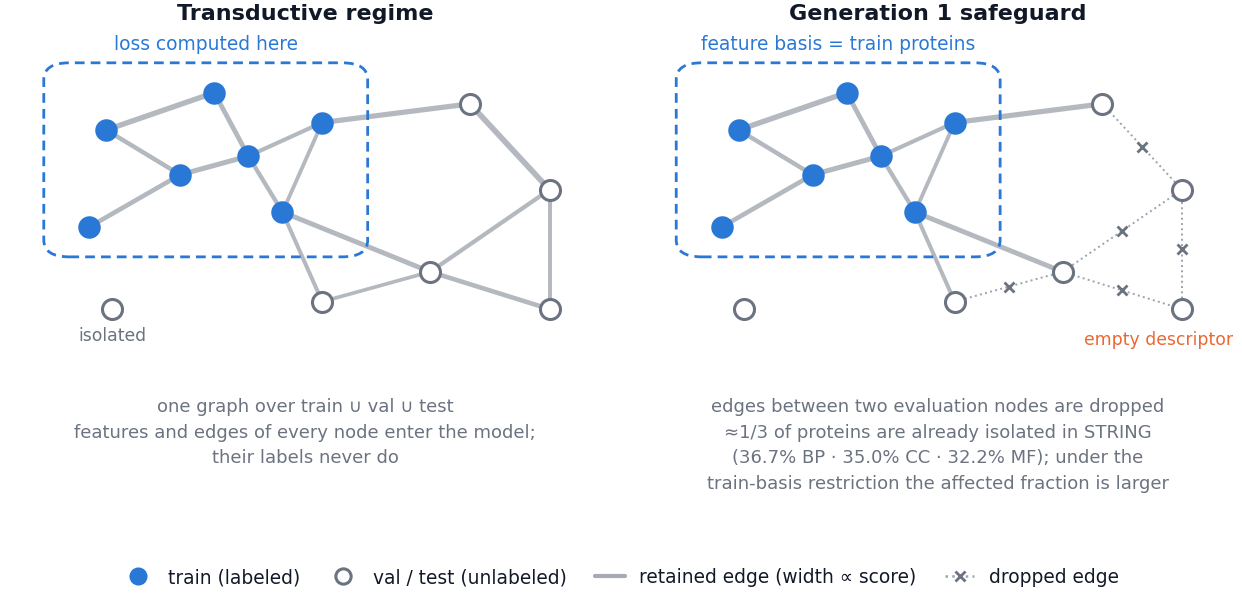
\includegraphics[width=\textwidth]{cap5/fig_5_02_learning_regime.png}
  \caption[Learning regime and supervision masking]{Learning regime. Left: the transductive regime
  used in the second generation (filled vertices are training proteins, hollow vertices are
  evaluation proteins that contribute attributes and edges but no labels, and the dashed boundary
  marks the vertices over which the loss of Equation~\eqref{eq:met_mascara} is computed). Right: the
  stricter train-basis construction of the first generation, in which edges incident to
  non-training proteins are discarded, so that an evaluation protein's descriptor is built only from
  training neighbors.}
  \label{fig:met_regime}
\end{figure}

This choice also has a direct consequence for the comparison reported in
Chapter~\ref{cap:resultados}. The five comparative methods evaluated in this work are
network-based methods that likewise operate over the complete vertex set; adopting a more
restrictive regime for the proposed models would produce numbers that measure the difference in
regime rather than the difference in method, and the final comparison would no longer be
interpretable. The two families nevertheless differ in the vertex universe they were originally
designed for and in the metric conventions they inherit, both documented in detail in
Appendix~\ref{ape:comparativos}; the first-generation experiments of
Section~\ref{sec:met_gen1} suffer from a comparable loss of information for a substantial
fraction of proteins, which Sections~\ref{sec:met_salvaguarda} and~\ref{sec:met_gen1_diag}
quantify. Neither point is developed further here.

\subsection{The Train-Basis Safeguard of the First Generation}
\label{sec:met_salvaguarda}

The first-generation experiments operate under a stricter regime. The vertex index is built over
the training identifiers only, and an interaction $(a,b)$ is registered exclusively when $b$
belongs to the training partition; each training protein additionally receives a self-connection
whose weight is set to the upper bound of the confidence scale, $0.999$, so that a protein is not
assigned a null score against itself. The coordinates of a protein's descriptor are therefore
indexed by training proteins,
and nothing else.

The consequence is that the protection extends beyond labels to the representation itself. In the
transductive regime of Section~\ref{sec:met_transdutivo}, an evaluation protein's representation may
be influenced by other evaluation proteins through the propagation operator, even though their
labels are never read. Under the train-basis construction that channel does not exist: an evaluation
protein is described only by its similarity to proteins whose annotations were available for
training, and no evaluation protein participates in the descriptor of another.

The price of this stricter construction is paid in coverage. Because the descriptor is a profile
over training neighbors, a protein whose interactions fall outside the training partition, or
which has no interaction above the confidence threshold, receives a descriptor that is
empty or nearly so. Section~\ref{sec:met_gen1_diag} quantifies the effect and shows why it is the
limitation that motivates the second generation.

\subsection{Model Selection and Reporting}
\label{sec:met_selecao}

Every model in this chapter is trained with early stopping, and the checkpoint retained for
evaluation is the one that minimizes the loss on the validation partition. The quantity of primary
interest in Chapter~\ref{cap:resultados} is $wF_{\max}$, not the validation loss, and
the two criteria do not necessarily reach their optimum at the same epoch. The convention adopted
here separates the two roles: the loss governs the choice of epoch within a configuration, and the
metric governs the comparison between configurations. The patience, the monitored quantity, and the
remaining optimization settings are reported in Appendix~\ref{ape:implementacao}.

All intermediate comparisons (e.g., between propagation operators, deduplication rules, prediction
heads, or fusion strategies) are decided on the validation partition. The test partition is read
once, in the final confrontation of Chapter~\ref{cap:resultados}, and is never consulted to select
a configuration. Each run predicts and stores the outputs for all three partitions in a single pass.

Finally, the experiments use a single random seed. The values reported are point estimates rather
than means over replicates, and no confidence interval is attached to them. The seeding mechanism,
including the determinization of the data-loading workers, is described in
Appendix~\ref{ape:implementacao}.

% =====================================================================
\section{First Generation}
\label{sec:met_gen1}

This section presents the models that represent a protein exclusively by its position in the STRING
network. All of them operate under the train-basis safeguard of Section~\ref{sec:met_salvaguarda},
and in all of them the edge weight of a pair is the largest confidence value reported for that pair,
so that weights remain in the interval $[0.400,\, 0.999]$ inherited from the combined score
(Section~\ref{sec:met_dedup} treats the deduplication question for the chapter as a whole).
Section~\ref{sec:met_baseline} first establishes what the topology yields with no learning at all;
Sections~\ref{sec:met_perfil} to~\ref{sec:met_heads_gen1} then follow the three-part decomposition
of Section~\ref{sec:met_overview}, and Section~\ref{sec:met_gen1_diag} states the limitation that
motivates the second generation. Figure~\ref{fig:met_gen1_pipeline} summarizes the routes described
below.

\begin{figure}[!htb]
  \centering
  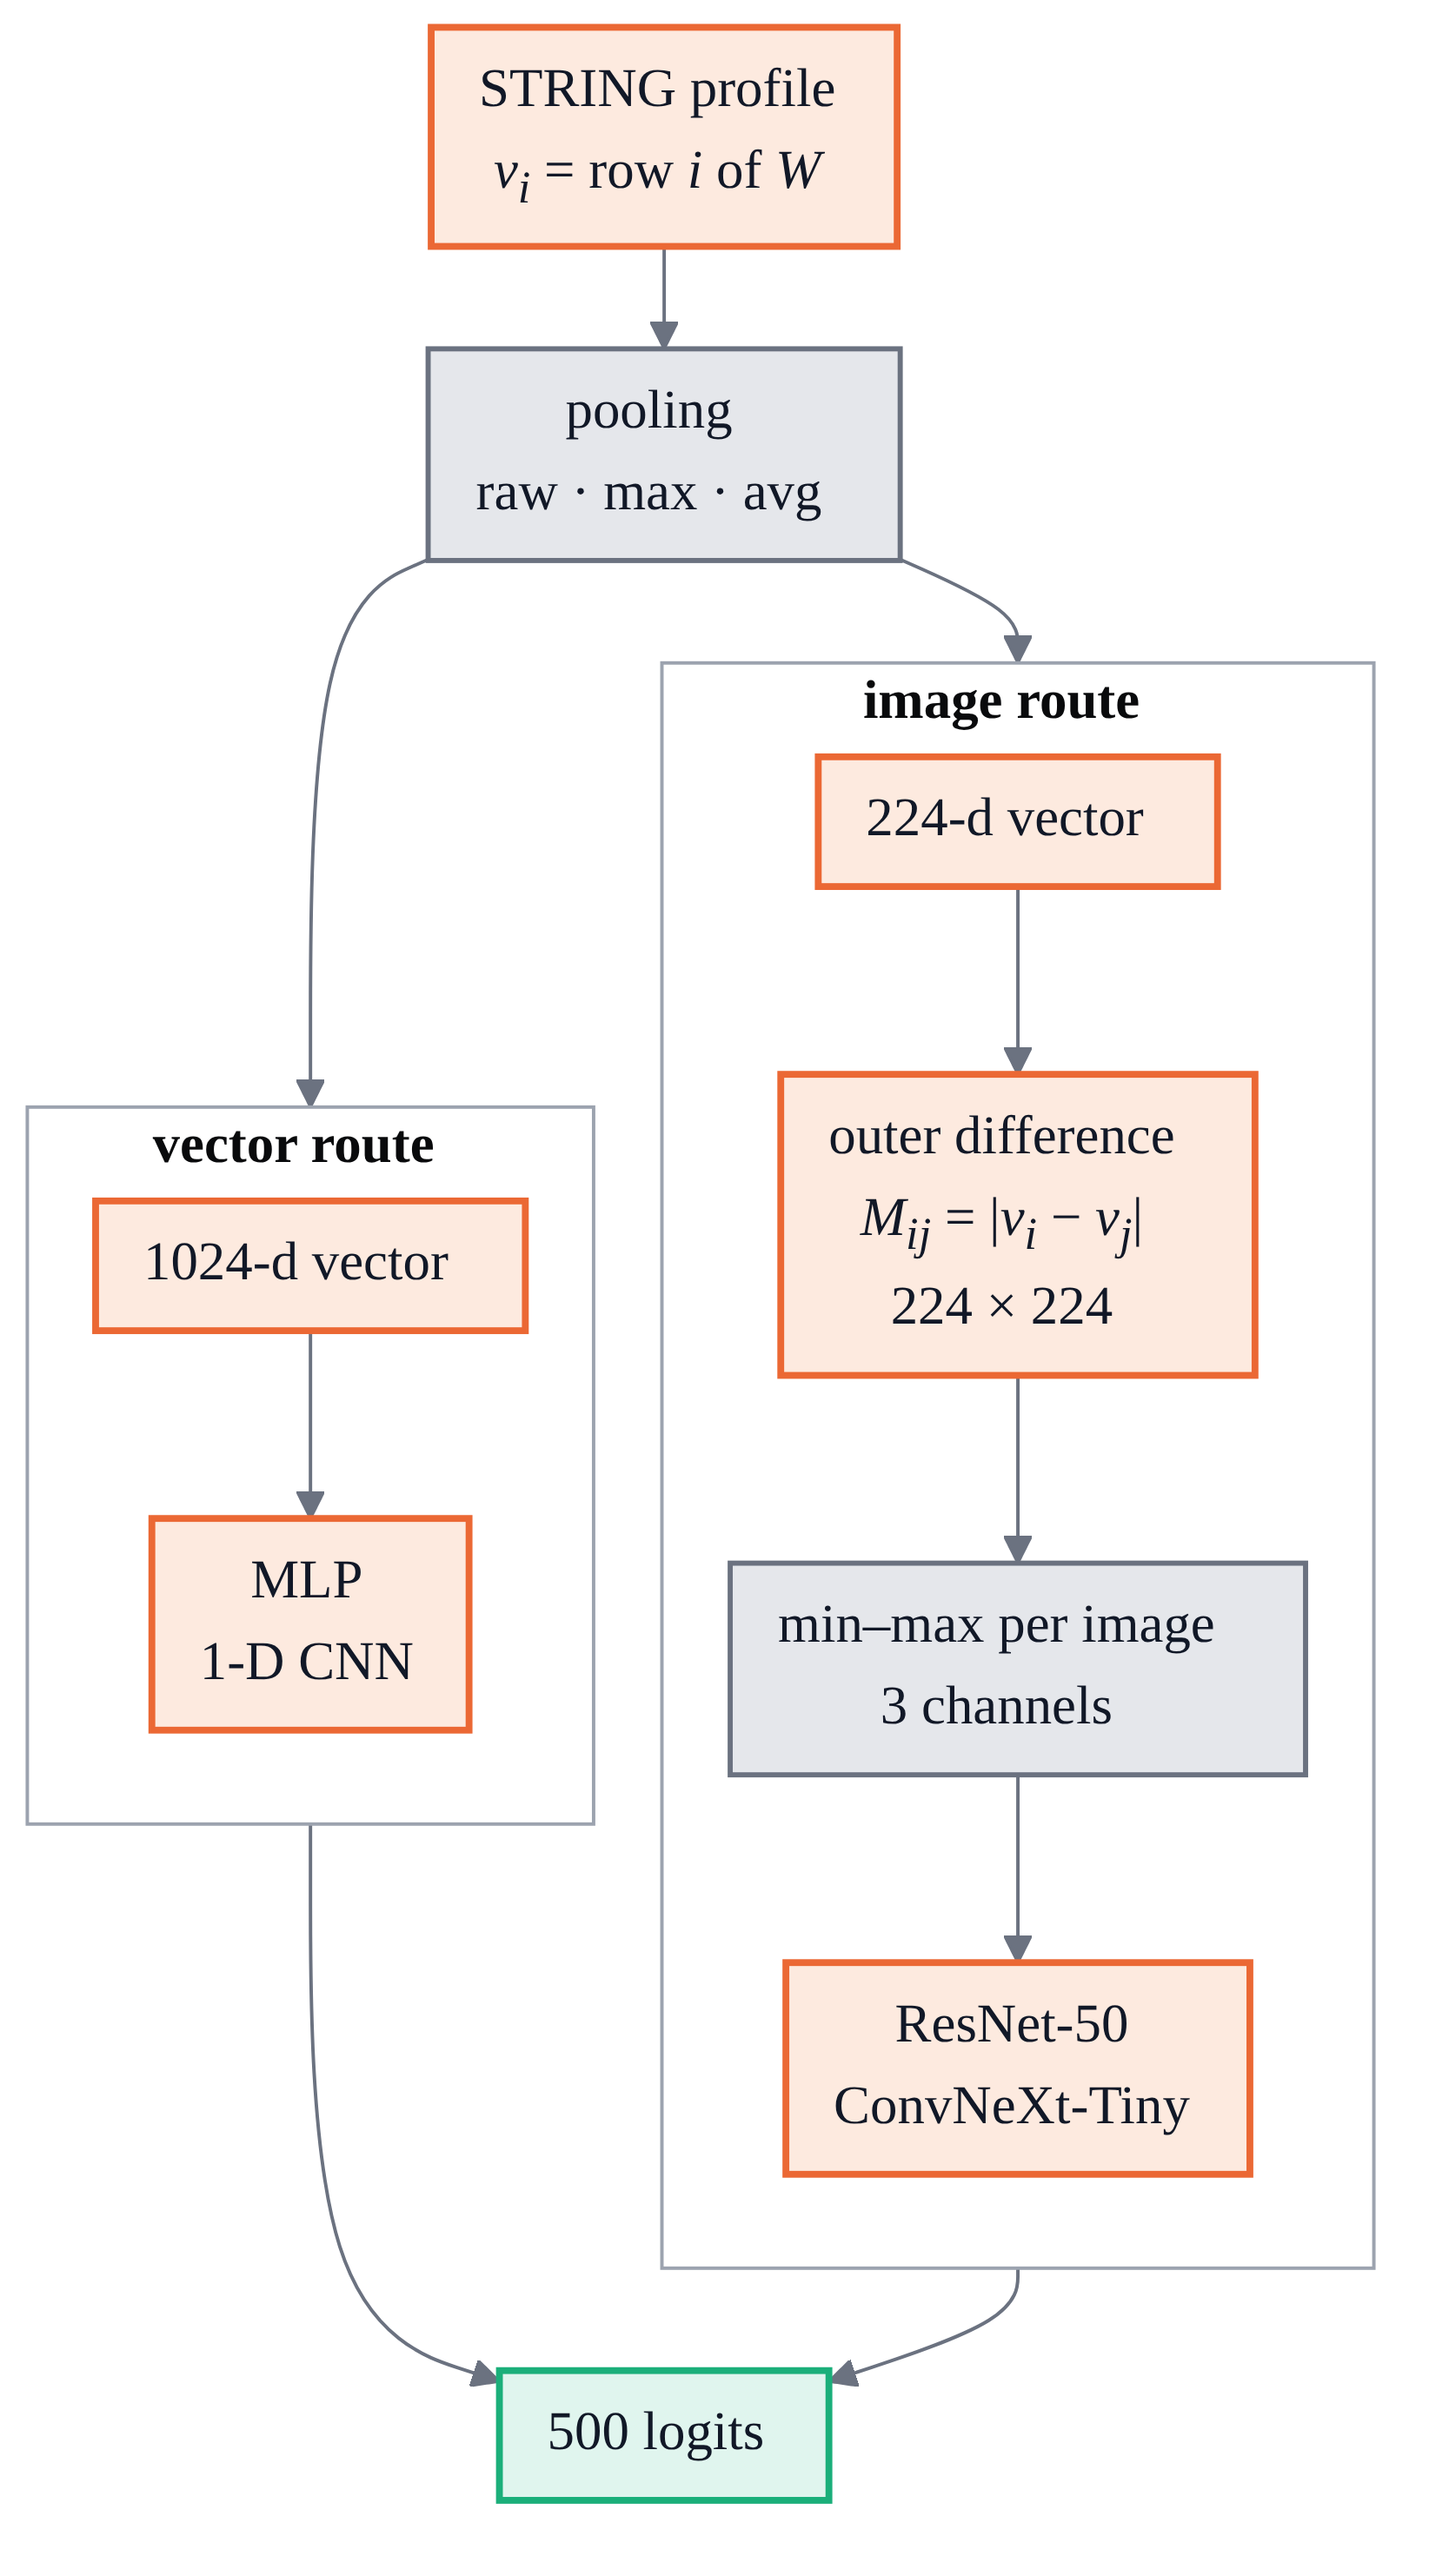
\includegraphics[width=0.6\textwidth]{cap5/fig_5_04_network_only_pipeline.png}
  \caption[First-generation pipeline]{First-generation pipeline. The STRING interaction profile is
  reduced by one of three pooling strategies and routed either to a vector head or, after the
  outer-difference construction, to a pretrained two-dimensional backbone. Both routes terminate in
  one logit per Gene Ontology term.}
  \label{fig:met_gen1_pipeline}
\end{figure}

\subsection{A Non-Parametric Naive Baseline}
\label{sec:met_baseline}

To establish the performance of the network topology without learning, a non-parametric naive baseline is
adopted based on a direct implementation of the guilt-by-association hypothesis
\cite{gillis2011impact}: the annotations of a protein are predicted as a confidence-weighted
combination of the annotations of its neighbors.

For a protein $i$ with neighborhood $\mathcal{N}(i)$ and interaction confidences $s_{ij}$, write
$\mathcal{N}_{\text{train}}(i) = \mathcal{N}(i) \cap \mathcal{V}_{\text{train}}$ for the subset of
its neighbors that belong to the training partition. The prediction is
\begin{equation}
  \hat{\mathbf{y}}_i \;=\;
  \begin{cases}
    \displaystyle\sum_{j \,\in\, \mathcal{N}_{\text{train}}(i)}
      \frac{s_{ij}}{\displaystyle\sum_{u \,\in\, \mathcal{N}_{\text{train}}(i)} s_{iu}}
      \;\, \mathbf{y}_j, & \mathcal{N}_{\text{train}}(i) \neq \varnothing, \\[16pt]
    \mathbf{0}, & \mathcal{N}_{\text{train}}(i) = \varnothing,
  \end{cases}
  \label{eq:met_baseline}
\end{equation}
\noindent where $\mathbf{y}_j$ is the binary annotation vector of training protein $j$. Restricting the
denominator to $\mathcal{N}_{\text{train}}(i)$ makes the coefficients sum to one over the neighbors
that actually contribute, which they would not do if neighbors outside the training partition
entered the normalization without entering the sum. The resulting score for a term lies in $[0,1]$
and is interpreted directly as a probability, without calibration.

The baseline has no trainable parameter and requires no optimization. It measures how much of the
annotation signal is recoverable from the weighted adjacency alone and establishes a floor against
which the models that follow can be read. It is evaluated through the same procedure as the trained
models, with the same hierarchical propagation of predictions and the same information content, so
its numbers are directly comparable to theirs.

\subsection{Representation}
\label{sec:met_perfil}

The descriptor of protein $i$ is the corresponding row of the weighted adjacency matrix restricted
to the training basis,
\begin{equation}
  \mathbf{v}_i \;=\; \left[\, w_{i1},\; w_{i2},\; \dots,\; w_{iN_{\text{train}}} \,\right],
  \qquad
  w_{ij} \in [0.400,\,0.999] \;\cup\; \{0\},
  \label{eq:met_perfil}
\end{equation}
\noindent where a zero coordinate denotes the absence of an interaction above the threshold. Three
conventions fix this vector. Its coordinates are indexed by the training identifiers in the order in
which they occur in the training partition file, an ordering recorded with the code so that a
profile
can be reconstructed; a pair reported more than once contributes the maximum of its confidences, so
that $w_{ij}$ is a single value in the range of the combined score; and only neighbors belonging to
the training partition are registered, as established in Section~\ref{sec:met_salvaguarda}. The
vector is extremely sparse, since the number of interaction partners of a protein is smaller than
the
number of training proteins by several orders of magnitude, and its dimension equals the number of
training proteins, which is on the order of tens of thousands. Two reductions are therefore
considered.

The first, denoted \texttt{raw}, keeps the full profile and lets the prediction head absorb the
dimensionality. The remaining two apply a window reduction along the profile, taking either the
maximum (\texttt{max}) or the average (\texttt{avg}) within each window, and produce a fixed-length vector. Two output lengths
are used, and they belong to different routes rather than being alternatives for the same route:
the vector route of Section~\ref{sec:met_gen1_vetor} consumes a $1024$-dimensional profile, and the
image route of Section~\ref{sec:met_gen1_img} consumes a $224$-dimensional profile, because $224$
is the side of the matrix it constructs. The three reduction strategies are design choices; their
relative behavior is examined in Chapter~\ref{cap:resultados}.

The window reduction is not adaptive. For a target length $L$ the window is fixed at
$k = \lfloor N_{\text{train}} / L \rfloor$ coordinates and applied with a stride equal to $k$ and no
padding, so the reduction emits $\lfloor (N_{\text{train}} - k)/k \rfloor + 1$ values. That count
coincides with $L$ only when $N_{\text{train}}$ is near a multiple of $L$; when it exceeds $L$ the
trailing values are dropped to bring the vector to length $L$, and were it to fall short the vector
would be completed by cycling over itself. At $L = 224$ the counts coincide in the three ontologies,
so the image route discards nothing. At $L = 1024$ they coincide for Biological Process and exceed
the target by eight and by seven coordinates for Cellular Component and Molecular Function, whose
last windows are therefore dropped. A window holding no interaction reduces to zero under both
operators, which the head cannot distinguish from a window whose interactions all fall below the
confidence threshold.

The ordering of the training identifiers is arbitrary with respect to the biology, so a window
reduction groups proteins that have no topological relation to one another. It is nevertheless fixed
and recorded, because the reduced profile, and therefore every downstream result, depends on it: two
runs under different orderings of the same identifiers would produce different vectors from the same
graph.

\subsection{Propagation}
\label{sec:met_prop_gen1}

In the first generation there is no propagation stage distinct from the representation. The
descriptor of Equation~\eqref{eq:met_perfil} is already an aggregation over the neighborhood of a
protein, since its nonzero coordinates are exactly the training partners of that protein and their
confidences; the network therefore enters the model once, as the input, and is not applied again
afterwards. The propagation is fixed at a single hop, it carries no parameter, and it cannot be
varied independently of the descriptor.

The baseline of Section~\ref{sec:met_baseline} is the degenerate case of that same one-hop
aggregation, applied to the annotation vectors of the neighbors rather than to the confidences, and
consumed directly as a prediction with no head at all. Separating the two roles the network plays
here, that of supplying the representation and that of modifying it, is precisely what the second
generation does, and it is what makes the number of hops and the retention coefficient of
Section~\ref{sec:met_fixa} free quantities rather than properties of the input.

\subsection{Prediction Head}
\label{sec:met_heads_gen1}

Two families of head consume the reduced profile: a vector family, which treats the profile as a
one-dimensional array, and an image family, which converts it into a two-dimensional array so that
convolutional backbones pretrained on natural images can be applied to it.

\subsubsection{Vector Heads}
\label{sec:met_gen1_vetor}

The first head is a multilayer perceptron with two fully connected hidden layers, each followed by a
rectified linear activation and dropout, terminating in a linear layer that emits one logit per Gene
Ontology term. It carries no normalization layer, in contrast with the head of the second generation
described in Section~\ref{sec:met_head_vetor}. The second is a one-dimensional convolutional
network that treats the
profile as an ordered signal.

As established in Section~\ref{sec:met_perfil}, the ordering of the profile coordinates carries no
meaning, leaving the convolution along that axis without a valid notion of locality to exploit.
The one-dimensional convolutional head is evaluated to determine whether the regularization and
reduced parameter count of weight sharing compensate for the absence of local structure.

\subsubsection{Image Route}
\label{sec:met_gen1_img}

Given a reduced profile $\mathbf{v} \in \mathbb{R}^{224}$, the outer-difference matrix is
\begin{equation}
  M_{ij} \;=\; \bigl| v_i - v_j \bigr|,
  \qquad
  M \in \mathbb{R}^{224 \times 224},
  \label{eq:met_outerdiff}
\end{equation}
\noindent which is non-negative and symmetric, and has a null diagonal. Its entry $(i,j)$ measures the absolute
difference between the interaction scores held at coordinates $i$ and $j$ of the profile; a protein
whose interactions are concentrated on few partners produces a matrix with pronounced structure,
whereas a protein with a flat profile produces a nearly uniform matrix.

The matrix is then brought to the input domain expected by the backbones. Writing
$m_{\min} = \min_{p,q} M_{pq}$ and $m_{\max} = \max_{p,q} M_{pq}$, a per-image min--max rescaling is
applied first,
\begin{equation}
  R_{ij} \;=\;
  \begin{cases}
    \dfrac{M_{ij} - m_{\min}}{m_{\max} - m_{\min}}, & m_{\max} > m_{\min}, \\[10pt]
    0, & \text{otherwise},
  \end{cases}
  \qquad
  \tilde{M}_{ij} \;=\; 2 R_{ij} - 1 \;\in\; [-1,\,1],
  \label{eq:met_imgnorm}
\end{equation}
\noindent where the second branch is the convention of the library routine used and covers the degenerate case
of a constant matrix, for which the rescaling would otherwise divide by zero.

In the implementation, the first stage is quantized to the $8$-bit integer range $[0,255]$ before the affine map to
$[-1,1]$, so a constant matrix, and in particular the null matrix of an isolated protein, is mapped
to the uniform array $\tilde{M} \equiv -1$. The result is finally replicated across three identical
channels, since the pretrained backbones expect a three-channel input. No resampling takes place at
any point: the profile is reduced to the side length the backbone expects, so the matrix is
constructed at that size and reaches the backbone unchanged in resolution.
Figure~\ref{fig:met_outerdiff} illustrates the sequence.

\begin{figure}[!htb]
  \centering
  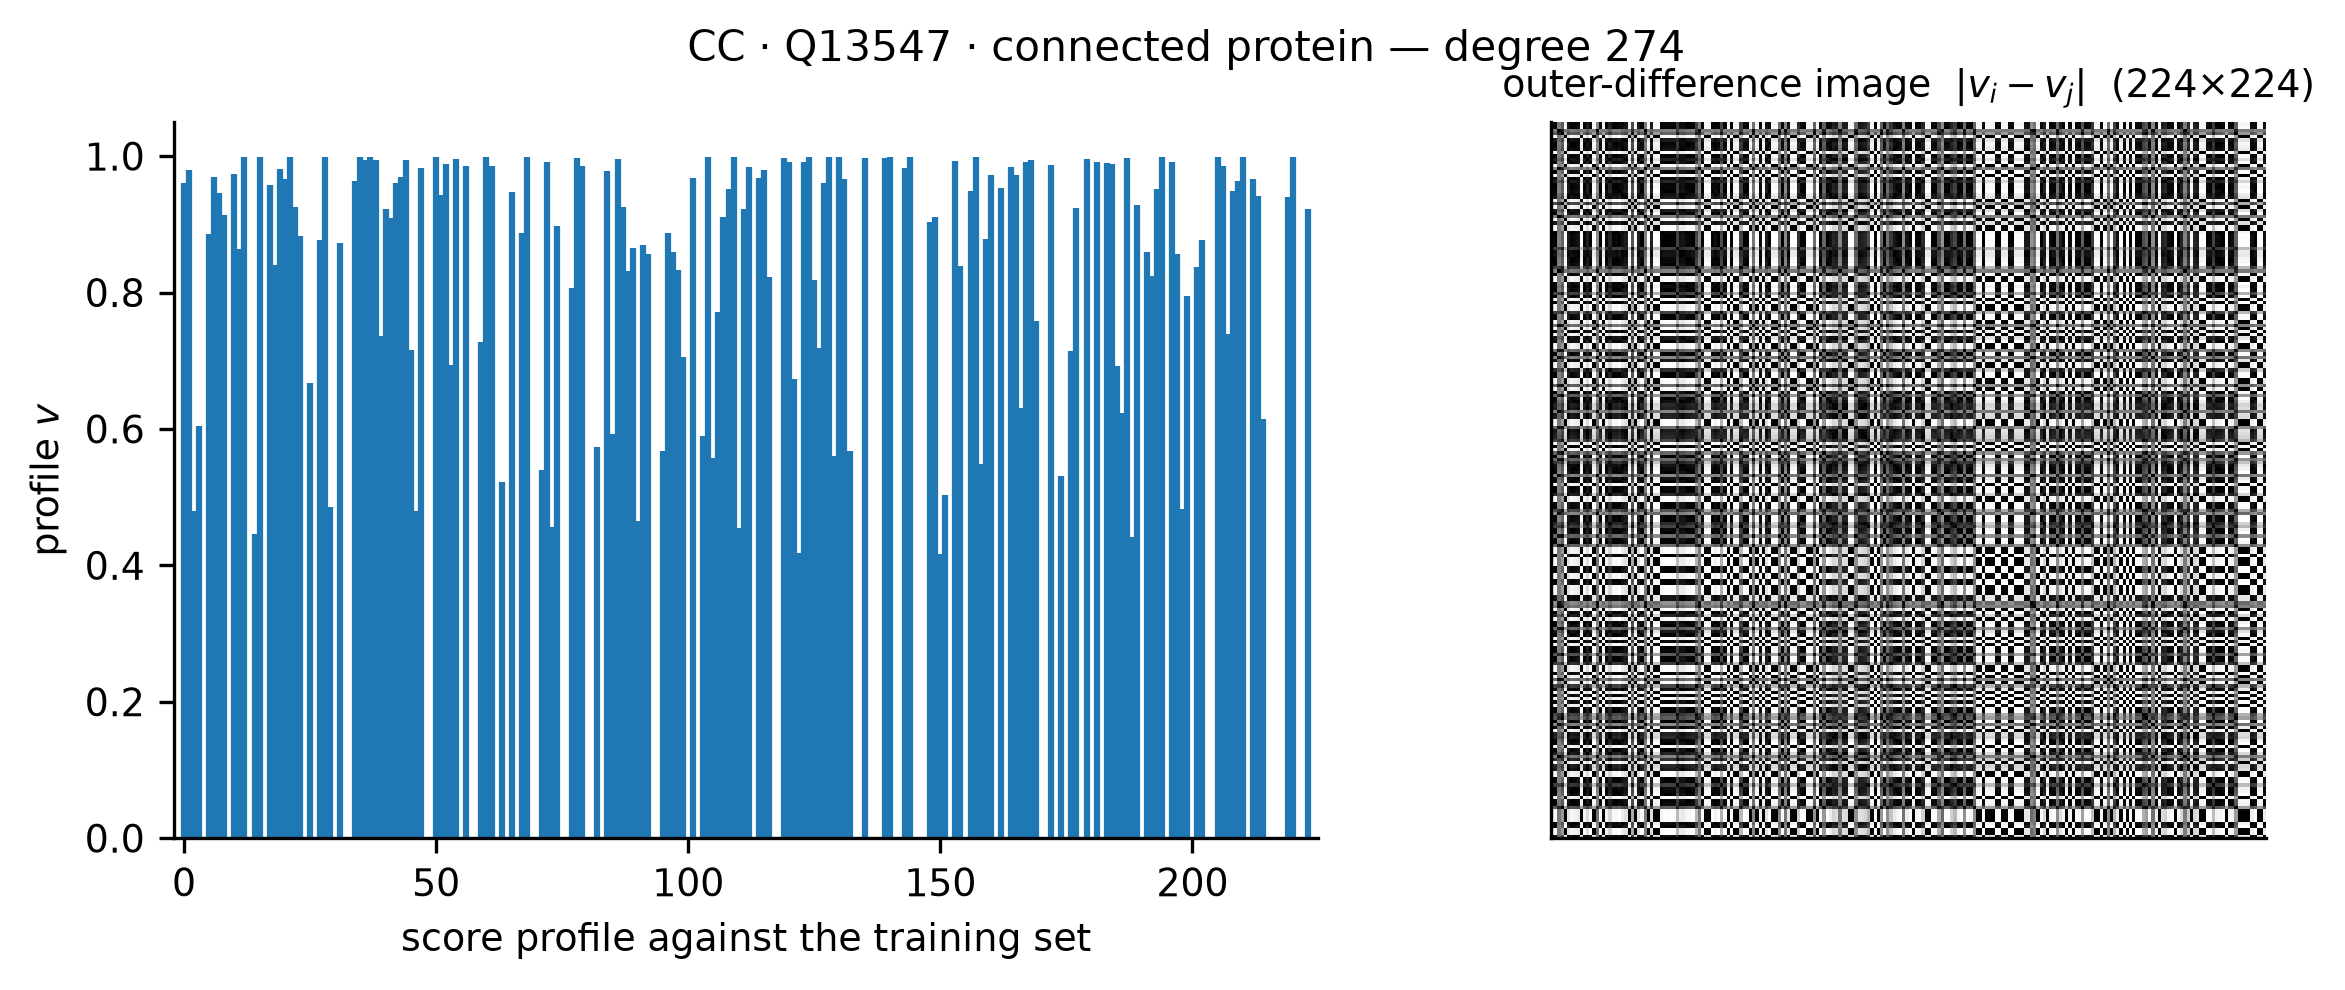
\includegraphics[width=\textwidth]{cap5/fig_5_03_outer_difference.png}
  \caption[Construction of the outer-difference image]{Construction of the outer-difference image,
  for a Cellular Component protein of degree $274$. Left: the interaction profile
  $\mathbf{v}$ of Equation~\eqref{eq:met_perfil}, reduced to $224$ coordinates, whose zero entries
  are the windows of training proteins containing no retained interaction with this one. Right: the matrix
  $M_{ij}=|v_i-v_j|$ of Equation~\eqref{eq:met_outerdiff}, symmetric with a null diagonal, after the
  per-image min--max rescaling of Equation~\eqref{eq:met_imgnorm}. The matrix is replicated across
  three identical channels before reaching the backbone.}
  \label{fig:met_outerdiff}
\end{figure}

The min--max rescaling is applied per image rather than with statistics shared across the dataset.
This preserves the relative contrast within each protein's own profile, which is the signal the
backbone is meant to detect, and it discards the absolute scale that would allow two proteins to be
compared by the magnitude of their interaction confidences. Given that the profiles differ
enormously in sparsity, normalizing within each image keeps weakly connected proteins from being
rendered as near-black inputs.

Two backbones are used, both pretrained on ImageNet~\cite{russakovsky2015imagenet}: ResNet-50
\cite{he2016deep} and ConvNeXt-Tiny~\cite{liu2022convnet}. These are the same two backbones reused
by the vision head of the second generation in Section~\ref{sec:met_head_visao}. Three decisions
apply to both routes. The stem of each backbone is left unmodified, and its final classification
layer is replaced by a linear layer emitting one score per retained Gene Ontology term. All weights
are then unfrozen and updated during training, the pretrained values acting as an initialization
rather than as a fixed feature extractor; partially frozen configurations were examined in
preliminary runs and are not part of the campaign reported in Chapter~\ref{cap:resultados}. And the
input is not standardized with the ImageNet channel statistics: here the matrix is rescaled to
$[-1,1]$ by Equation~\eqref{eq:met_imgnorm}, and in
Section~\ref{sec:met_head_visao} the values are already bounded by a logistic map. There is no
semantic correspondence between natural images and interaction matrices, and no claim of one is made
here; what transfer is expected to provide is a set of filters tuned to detect local structure (such
as edges, blocks, or repeated patterns) present in the outer-difference matrix. The route is an
exploratory representation choice.

\subsection{Limitations}
\label{sec:met_gen1_diag}

The first generation is bounded by a property of its input rather than by the capacity of its heads.
Approximately one third of the proteins in each ontology have no interaction above the confidence
threshold: $36.65\%$ in Biological Process, $34.95\%$ in Cellular Component and $32.19\%$ in
Molecular Function. For such a protein, Equation~\eqref{eq:met_perfil} returns the null vector,
Equation~\eqref{eq:met_outerdiff} returns the null matrix, and after the per-image rescaling of
Equation~\eqref{eq:met_imgnorm} the input becomes a uniform array carrying no information about the
protein. The head can only respond with the class prior it has learned. Under the train-basis
safeguard of Section~\ref{sec:met_salvaguarda} the affected fraction is larger still, because a
protein whose neighbors all fall outside the training partition is in the same position as an
isolated one. Figure~\ref{fig:met_isolated} shows the contrast.

\begin{figure}[!htb]
  \centering
  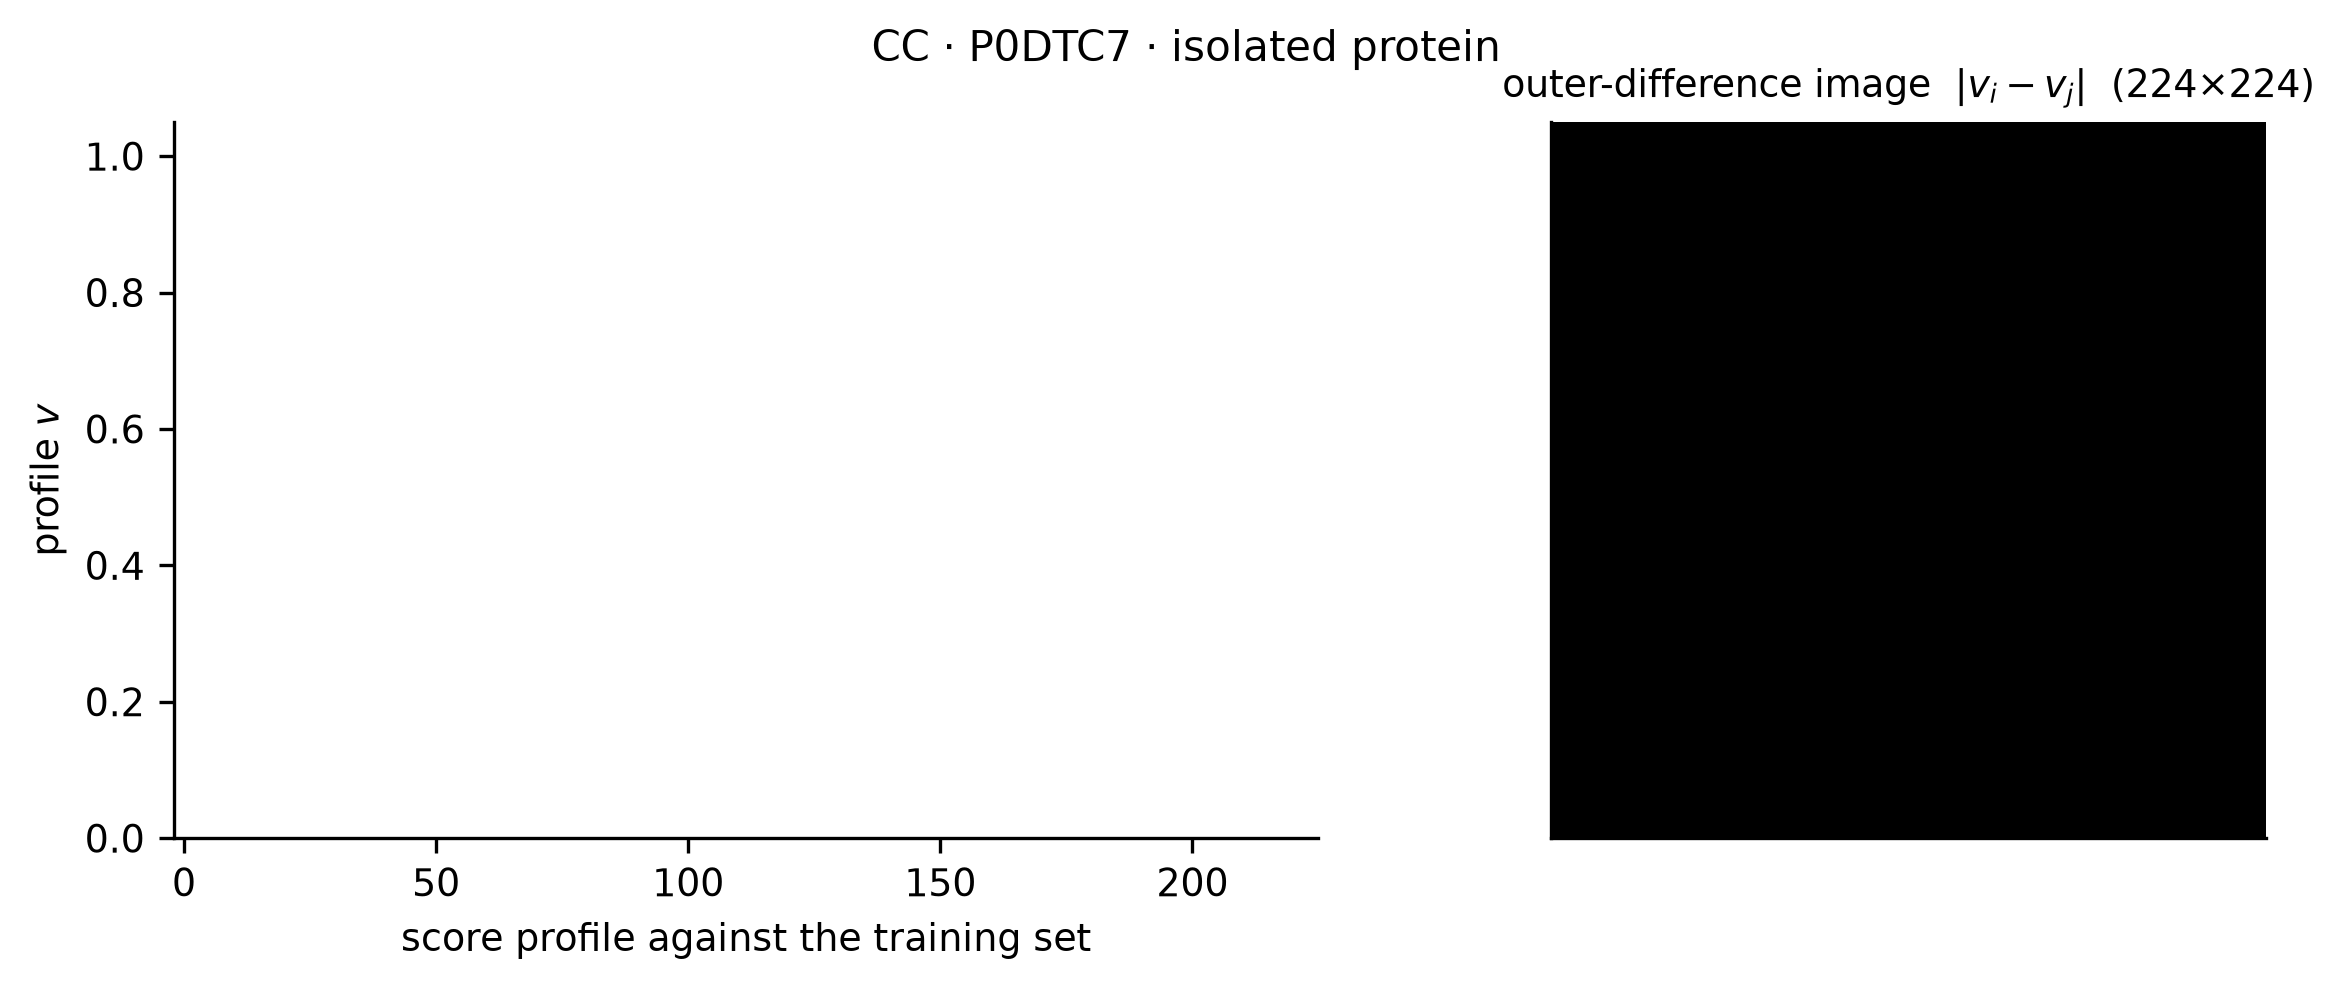
\includegraphics[width=\textwidth]{cap5/fig_5_05_isolated_vs_connected.png}
  \caption[An isolated protein under the first-generation representation]{The construction of
  Figure~\ref{fig:met_outerdiff} applied to an isolated Cellular Component protein. The profile is
  null at every coordinate, so the outer-difference matrix is null as well and the resulting image is
  uniform. The two figures are drawn on the same scale: the input the head receives for this protein
  carries no information about it, and no choice of architecture can recover what is absent.}
  \label{fig:met_isolated}
\end{figure}

No choice of pooling, of architecture or of objective can repair this, because the information is
absent from the representation. What the observation does establish is the requirement for the
second generation: the representation must be available for every protein, including those
the network does not reach. The amino-acid sequence satisfies that requirement by construction, and
it is the starting point of Section~\ref{sec:met_repr}.


% =====================================================================
\section{Second Generation}
\label{sec:met_repr}

The second generation separates the two roles that the network played in the first. The
representation of a protein is now derived from its amino-acid sequence, and the network becomes an
operator that modifies that representation according to the protein's neighborhood. This separation
is what makes the representation available for isolated proteins, and it is also what allows the
propagation mechanism to be studied independently of the descriptor. The section follows the same
three-part decomposition as Section~\ref{sec:met_gen1}, and Figure~\ref{fig:met_hybrid_pipeline}
gives the complete flow.

\begin{figure}[!htb]
  \centering
  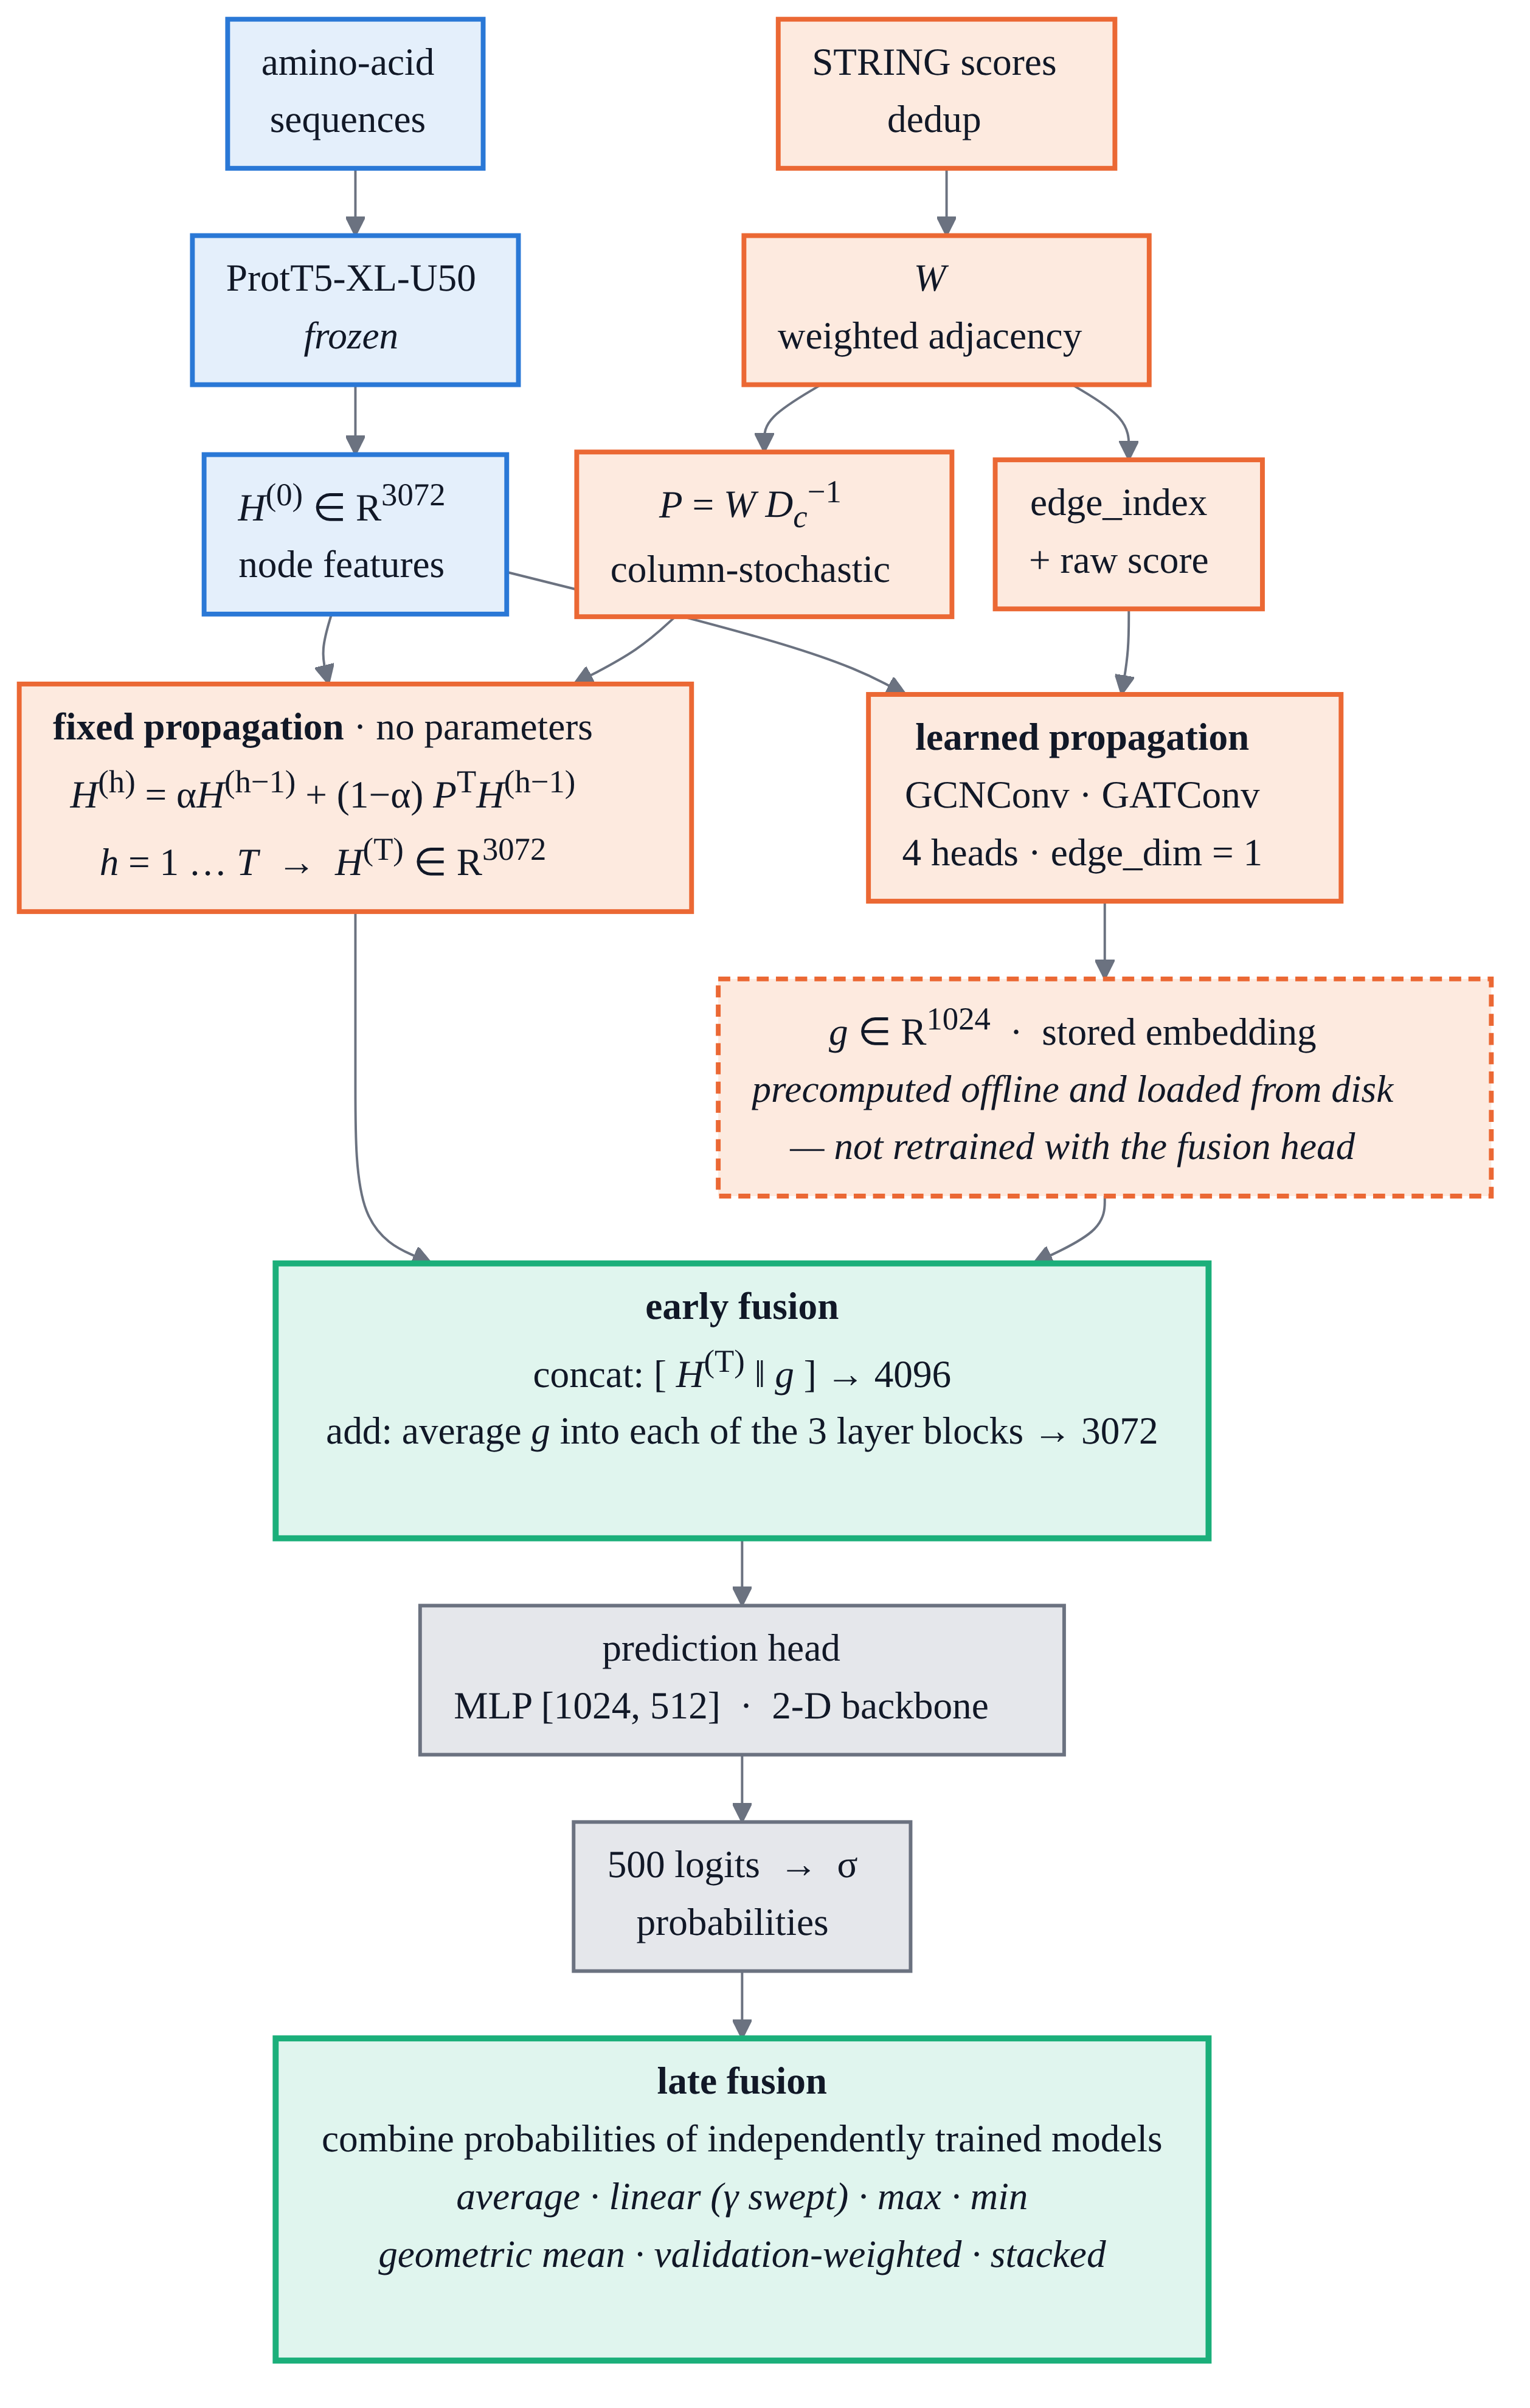
\includegraphics[width=0.6\textwidth]{cap5/fig_5_06_hybrid_pipeline.png}
  \caption[Second-generation pipeline]{Second-generation pipeline. Sequence embeddings and the
  weighted interaction graph enter as separate inputs; propagation is performed either by the fixed
  operator of Equation~\eqref{eq:met_recorrencia} or by a learned graph convolution; the resulting
  representations are combined by early fusion before a single head, or the resulting probabilities
  are combined by late fusion after independent training.}
  \label{fig:met_hybrid_pipeline}
\end{figure}

\subsection{Representation}
\label{sec:met_repr_g2}

The representation of the second generation has two components: a per-protein vector derived from
the sequence, which becomes the node attribute, and the weighted graph over which that attribute is
later propagated. The two are specified in turn, followed by the rule that reduces the repeated
interaction records of a pair to a single edge weight.

\subsubsection{Sequence Embeddings}
\label{sec:met_prott5}

Node attributes are extracted with ProtT5-XL-U50~\cite{elnaggar2021prottrans}, a T5
encoder-decoder trained on protein sequences with a BART-like denoising objective that masks
$15\%$ of the residues individually, rather than with the span-corruption objective of the
original T5; the checkpoint was initialized from the model pretrained on BFD and subsequently
trained on UniRef50. Only the encoder is used here, and its weights remain frozen: the model acts
as a fixed feature extractor, and no gradient from the function prediction task reaches it.
 
Following the extraction pipeline inherited without modification from SUPERMAGOv2
(Appendix~\ref{ape:prott5}), a protein $i$ longer than $1{,}022$ tokens is split into
$K_i$ consecutive chunks and each chunk is encoded independently. This preserves local context
within
each chunk at the cost of severing the attention pathway at the chunk boundaries; the alternative
(truncating long sequences) would discard entire domains, which is the less acceptable of the two
losses in a function prediction task.

Three hidden layers are read: the last layer of the encoder, $\ell = 24$, and its two predecessors,
$\ell = 23$ and $\ell = 22$. Each yields a $1024$-dimensional vector per residue, and each is
reduced
to a single protein-level vector in two stages. Within a chunk, the per-residue hidden states are
averaged over the valid positions, with the padding excluded by the attention mask; across chunks,
the resulting chunk-level vectors are averaged with equal weight:
\begin{equation}
  \mathbf{e}^{(\ell)}_i \;=\; \frac{1}{K_i} \sum_{k=1}^{K_i}
  \left( \frac{1}{|\mathcal{A}_{ik}|}
  \sum_{t \,\in\, \mathcal{A}_{ik}} \mathbf{h}^{(\ell)}_{ik,t} \right),
  \qquad \ell \in \{22,\,23,\,24\},
  \label{eq:met_meanpool}
\end{equation}
\noindent where $\mathcal{A}_{ik}$ is the set of residue positions of the $k$-th chunk of protein $i$ retained
by the attention mask. The two stages are not equivalent to a single average over all residues: the
outer mean weights every chunk equally, so the residues of a short trailing chunk carry more weight
per residue than those of a full one. For a protein short enough to fit in a single chunk, $K_i = 1$
and the two stages collapse into the masked mean over its residues.
The three vectors are concatenated, from the deepest layer to the shallowest, so that the first
$1024$ coordinates of $\mathbf{H}^{(0)}$ correspond to layer $24$, to form the node attribute matrix
of the graph:
\begin{equation}
  \mathbf{H}^{(0)}_i \;=\;
  \left[\, \mathbf{e}^{(24)}_i \;\big\|\; \mathbf{e}^{(23)}_i \;\big\|\; \mathbf{e}^{(22)}_i \,\right]
  \;\in\; \mathbb{R}^{3072}.
  \label{eq:met_h0}
\end{equation}

Three layers are read rather than one for the following reason. The final layer of a masked language
model is the most specialized toward its pretraining objective, whereas intermediate layers retain
signal that is less task-specific and, in protein language models, more closely associated with
structural properties. Selecting a single layer would require committing to one point on that
spectrum; concatenating three adjacent layers keeps the information available to the downstream head
without introducing a parameter to be tuned, at the cost of tripling the attribute dimension.
Figure~\ref{fig:met_prott5} summarizes the extraction. The operational aspects (numerical precision,
batching, extraction time, and the on-disk layout of one file per layer per protein) are reported in
Appendix~\ref{ape:implementacao}.

\begin{figure}[!htb]
  \centering
  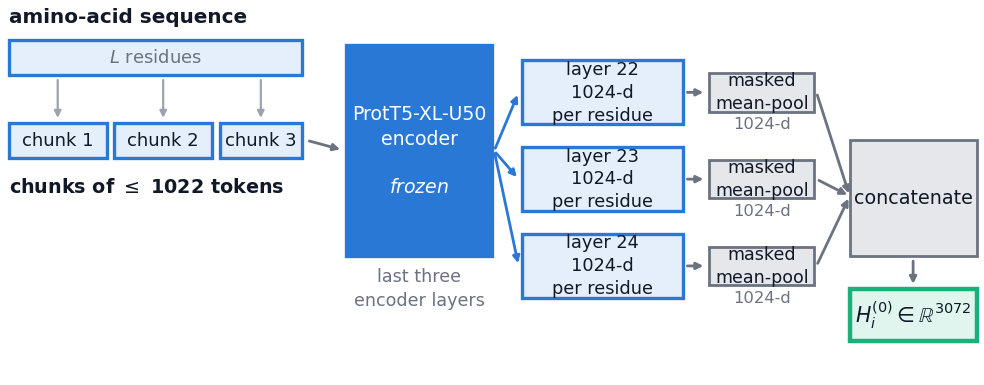
\includegraphics[width=\textwidth]{cap5/fig_5_07_prott5_extraction.png}
  \caption[Extraction of the sequence representation]{Extraction of the sequence representation. The
  amino-acid sequence is split into chunks of at most $1{,}022$ tokens and encoded by the frozen
  ProtT5-XL-U50 encoder; layers $24$, $23$ and $22$ are read, mean-pooled over the valid residue
  positions as in Equation~\eqref{eq:met_meanpool}, and concatenated in that order into the
  $3072$-dimensional node attribute of Equation~\eqref{eq:met_h0}.}
  \label{fig:met_prott5}
\end{figure}

\subsubsection{The Interaction Graph}
\label{sec:met_grafo}

The provenance of the interaction data, the composition of the STRING combined score, and the
confidence threshold adopted are described in Chapter~\ref{cap:materiais} and are not repeated here.
This part specifies how that data becomes the operator used by the propagation step.

Each retained interaction contributes a symmetric pair of entries, so the weight matrix
$W \in \mathbb{R}^{|\mathcal{V}| \times |\mathcal{V}|}$ is symmetric by construction; pairs whose two
endpoints coincide are discarded, so $W$ has a null diagonal and the graph carries no self-loops.
Writing $m$ for the number of undirected edges, the number of stored entries is
$\operatorname{nnz}(W) = 2m$, and the two quantities are kept distinct throughout: the graphs
contain
$m = 492{,}920$ undirected edges for Biological Process, $566{,}566$ for Cellular Component and
$470{,}206$ for Molecular Function.

\paragraph{Sparse Representation.} Neither $W$ nor the operator derived from it is ever materialized
as a dense array. With $|\mathcal{V}|$ on the order of $10^5$, a dense matrix would occupy between
$25$ and $35$~GB in single precision, depending on the ontology, whereas the number of stored
entries does not exceed $1{,}133{,}132$, which is the Cellular Component graph and corresponds to a
density of $1.31 \times 10^{-4}$; the densest of the three graphs, Molecular Function, reaches
$1.52 \times 10^{-4}$. The graph is therefore held in coordinate format (\textsc{coo}): an integer
index tensor of shape $2 \times \operatorname{nnz}(W)$ paired with a value tensor of the same
length,
from which a sparse tensor is assembled.

The reduction of the repeated records is explicit rather than delegated to the sparse-tensor
machinery, and the order matters, because the coalescing routines of a tensor library sum duplicate
entries by default and do not implement a maximum. Each surviving record of a pair emits its two
directed entries, $(i,j)$ and $(j,i)$, with the same value; the entries are then grouped by directed
index pair through a stable sort, and the deduplication rule defined below in this section, summation or maximum,
is applied within each group. Only then is the sparse tensor built, and the coalescing call it
receives serves solely to guarantee uniqueness, every duplicate having already been reduced.
Emitting both directions before the reduction keeps the operator symmetric under either rule, since
$(i,j)$ and $(j,i)$ accumulate the same multiset of records.

Propagation is then carried out by sparse-dense matrix multiplication, whose cost is proportional to
$\operatorname{nnz}(W)$ rather than to $|\mathcal{V}|^2$: the null entries are never visited, and
the
memory footprint of the operator remains linear in the number of edges. This is what makes the
propagation step of
Section~\ref{sec:met_fixa} tractable at the scale of the full corpus, and the same sparse
representation is consumed by the graph convolutions of Section~\ref{sec:met_gnn}.

\paragraph{Stochastic Normalization.} The weight matrix is normalized column-wise,
\begin{equation}
  P \;=\; W D_c^{-1},
  \qquad
  D_c \;=\; \operatorname{diag}\!\left(\max\Bigl\{\textstyle\sum_i W_{ij},\; \varepsilon\Bigr\}\right),
  \label{eq:met_P}
\end{equation}
\noindent so that every nonempty column of $P$ sums to one. The interpretation is that the weight a neighbor
receives is defined relative to the other neighbors of the same protein rather than on an
absolute scale: a confidence of $0.8$ counts for much in a protein with two partners and for little
in a protein with fifty. A protein with no retained interaction has a null column, for which the
sum would be zero; the floor $\varepsilon = 10^{-12}$ makes the inverse well defined and leaves the
corresponding column of $P$ null. The consequence of that for the propagation operator is stated in
Section~\ref{sec:met_fixa}.

\subsubsection{Edge Weighting and Deduplication}
\label{sec:met_dedup}

The interaction file inherited for this work lists $2{,}422{,}234$ records for $791{,}011$ distinct
protein pairs: each pair appears on average $3.06$ times, and up to $170$ times, always with an
identical score. As documented in Chapter~\ref{cap:materiais}, these are evidence records whose
discriminating column was lost when the file was assembled, and the combined score has already
aggregated the channels that produced them, so a repeated record does not constitute independent
corroboration. The coalescing pass described above must therefore reduce the repeated
records of a pair to a single weight, and the reduction operator is a methodological choice.

Many reductions are admissible in principle, among them the mean, the median, the minimum and the
mode. Two are evaluated here. Writing $s^{(k)}_{ij}$ for the score of the $k$-th record of the pair
$(i,j)$, with multiplicity $c_{ij}$ and common value $s_{ij}$,
\begin{equation}
  w^{\text{sum}}_{ij} \;=\; \sum_{k} s^{(k)}_{ij} \;=\; c_{ij}\, s_{ij},
  \qquad\qquad
  w^{\max}_{ij} \;=\; \max_{k} s^{(k)}_{ij} \;=\; s_{ij}.
  \label{eq:met_dedup}
\end{equation}

The two readings differ in what they take the repeated records to mean. Because all repeated
records of a pair carry the same combined score, the maximum rule does not select a strongest piece
of evidence: it preserves the pair-level score already aggregated by STRING, without reweighting it
by record multiplicity, and keeps the weight on the original scale of that score. Summation, in
contrast, multiplies the score by the number of inherited records and therefore treats multiplicity
as additional evidence; the weight then leaves the unit interval and becomes a product of count and
confidence, reaching $167.79$ in the Biological Process graph.

The choice is not neutralized by the normalization of Equation~\eqref{eq:met_P}. Because
multiplicity varies among the neighbors of the same protein, the two rules can reverse their
relative ordering: a neighbor repeated five times with score $0.80$ dominates a neighbor appearing
once with score $0.95$ under summation, and is dominated by it under the maximum. Both rules are
treated as admissible methodological paths in this dissertation, and both are evaluated in
Chapter~\ref{cap:resultados}.

\subsection{Propagation}
\label{sec:met_prop}

Both propagation routes considered here belong to the message-passing family: a protein's
representation is updated by aggregating the representations of its neighbors and combining the
result with its own. What distinguishes them is whether the aggregation weights are given by the
graph or estimated from the data, and whether the update carries trainable parameters. The two
routes are presented in turn, followed by the property they share and that bounds both.

\subsubsection{Fixed Propagation}
\label{sec:met_fixa}

The first route decouples propagation from learning entirely. The graph acts on the node attributes
before the prediction head, through a deterministic operator with no trainable parameter,
\begin{equation}
  \mathbf{H}^{(h)} \;=\; \alpha\, \mathbf{H}^{(h-1)}
  \;+\; (1-\alpha)\, P^{\top} \mathbf{H}^{(h-1)},
  \qquad h = 1, \dots, T,
  \label{eq:met_recorrencia}
\end{equation}
\noindent with $\mathbf{H}^{(0)}$ given by Equation~\eqref{eq:met_h0} and $\alpha \in [0,1]$. At each step the
coefficient $\alpha$ retains a fraction of the representation produced by the previous iteration,
not
of the original one: since that previous representation may already carry neighborhood information,
$\alpha$ slows the mixing rather than continuously reintroducing the sequence representation. The
transpose is what makes the second term an aggregation over
the neighbors of each protein: since Equation~\eqref{eq:met_P} normalizes $P$ by column, the
row $i$ of $P^{\top}\mathbf{H}$ is a convex combination of the attributes of the neighbors of $i$,
with coefficients summing to one. Writing the operator without the transpose would instead
distribute each protein's attribute to its neighbors, which is a different operation.

The recurrence has two degenerate settings. With $T = 0$, or equivalently with $\alpha = 1$, the
operator is the identity and $\mathbf{H}^{(T)} = \mathbf{H}^{(0)}$: the graph is switched off and the
model reduces to a head applied to the sequence representation alone. This configuration serves as
the internal control to isolate the topological contribution of the network from the
sequence-derived features, which is evaluated in Chapter~\ref{cap:resultados}.

Because the graph carries no self-loops (Section~\ref{sec:met_grafo}), the only self-connection in
Equation~\eqref{eq:met_recorrencia} is the explicit $\alpha$ term, and no self-loop is added to
compensate. For a protein with no retained interaction, the corresponding row of $P^{\top}$ is empty
and the recurrence reduces to $\mathbf{H}^{(h)}_i = \alpha\, \mathbf{H}^{(h-1)}_i$, so after $T$
steps the protein carries $\alpha^{T}\mathbf{H}^{(0)}_i$ rather than $\mathbf{H}^{(0)}_i$. The
scaling is uniform across the coordinates, so the direction of the representation is preserved,
but isolated proteins enter the head at a scale that depends on $\alpha$ and $T$ while connected
proteins do not. This is a structural property of the operator rather than a setting to be tuned,
and the learned route of Section~\ref{sec:met_gnn} does not share it. Consequently, for isolated proteins, a difference between a fixed-propagation configuration with $T > 0$ and the $T = 0$ control cannot be attributed to neighborhood information, because no such information is available. It may instead reflect the $\alpha^{T}$ rescaling of the representation and the retraining of the prediction head on the resulting input distribution. The operator is retained as implemented, while alternatives that preserve the initial representation exactly for isolated nodes are left for future work.


Equation~\eqref{eq:met_recorrencia} requires $T$ sparse-dense multiplications, involves no
parameter and therefore no gradient, and is independent of the prediction head; it is consequently
evaluated once per experiment, outside the training loop, and its result is cached and reused at
every epoch.

What the recurrence computes admits a closed form, and stating it settles both its relation to the
literature and the reading of $\alpha$. Collecting the two terms into a single operator
$Q = \alpha I + (1-\alpha) P^{\top}$ gives $\mathbf{H}^{(T)} = Q^{T} \mathbf{H}^{(0)}$, and since
$\alpha I$ commutes with $P^{\top}$ the binomial expansion is exact:
\begin{equation}
  \mathbf{H}^{(T)} \;=\; \sum_{k=0}^{T} \binom{T}{k}\, \alpha^{T-k} (1-\alpha)^{k}
  \bigl(P^{\top}\bigr)^{k} \mathbf{H}^{(0)}.
  \label{eq:met_binomial}
\end{equation}

The operator is therefore a finite-step lazy diffusion whose weights over hop counts are the
probability mass function of a binomial distribution with $T$ trials and success probability
$1-\alpha$: the mean number of hops is $T(1-\alpha)$, and the unpropagated term, $k=0$, carries
weight exactly $\alpha^{T}$. Lowering $\alpha$ shifts that mass toward deeper hops without changing
the number of steps.

This distinguishes the recurrence from the restart formulations it superficially resembles. Label
propagation with local and global consistency~\cite{zhou2004learning} and personalized-PageRank
propagation~\cite{klicpera2019predict} reinject the initial label or prediction matrix at every
iteration, which anchors their fixed point to that initial state;
Equation~\eqref{eq:met_recorrencia}
never reinjects it, so it does not share that fixed point. It sits closer to the decoupled
formulations that apply fixed powers of a normalized graph operator before a conventional predictor
\cite{wu2019simplifying}, from which it differs in the object being propagated, a concatenation of
embeddings read from three layers of a protein language model, and in the graph over which the
propagation runs.
Figure~\ref{fig:met_fixa} illustrates the effect of the two coefficients.

\begin{figure}[!htb]
  \centering
  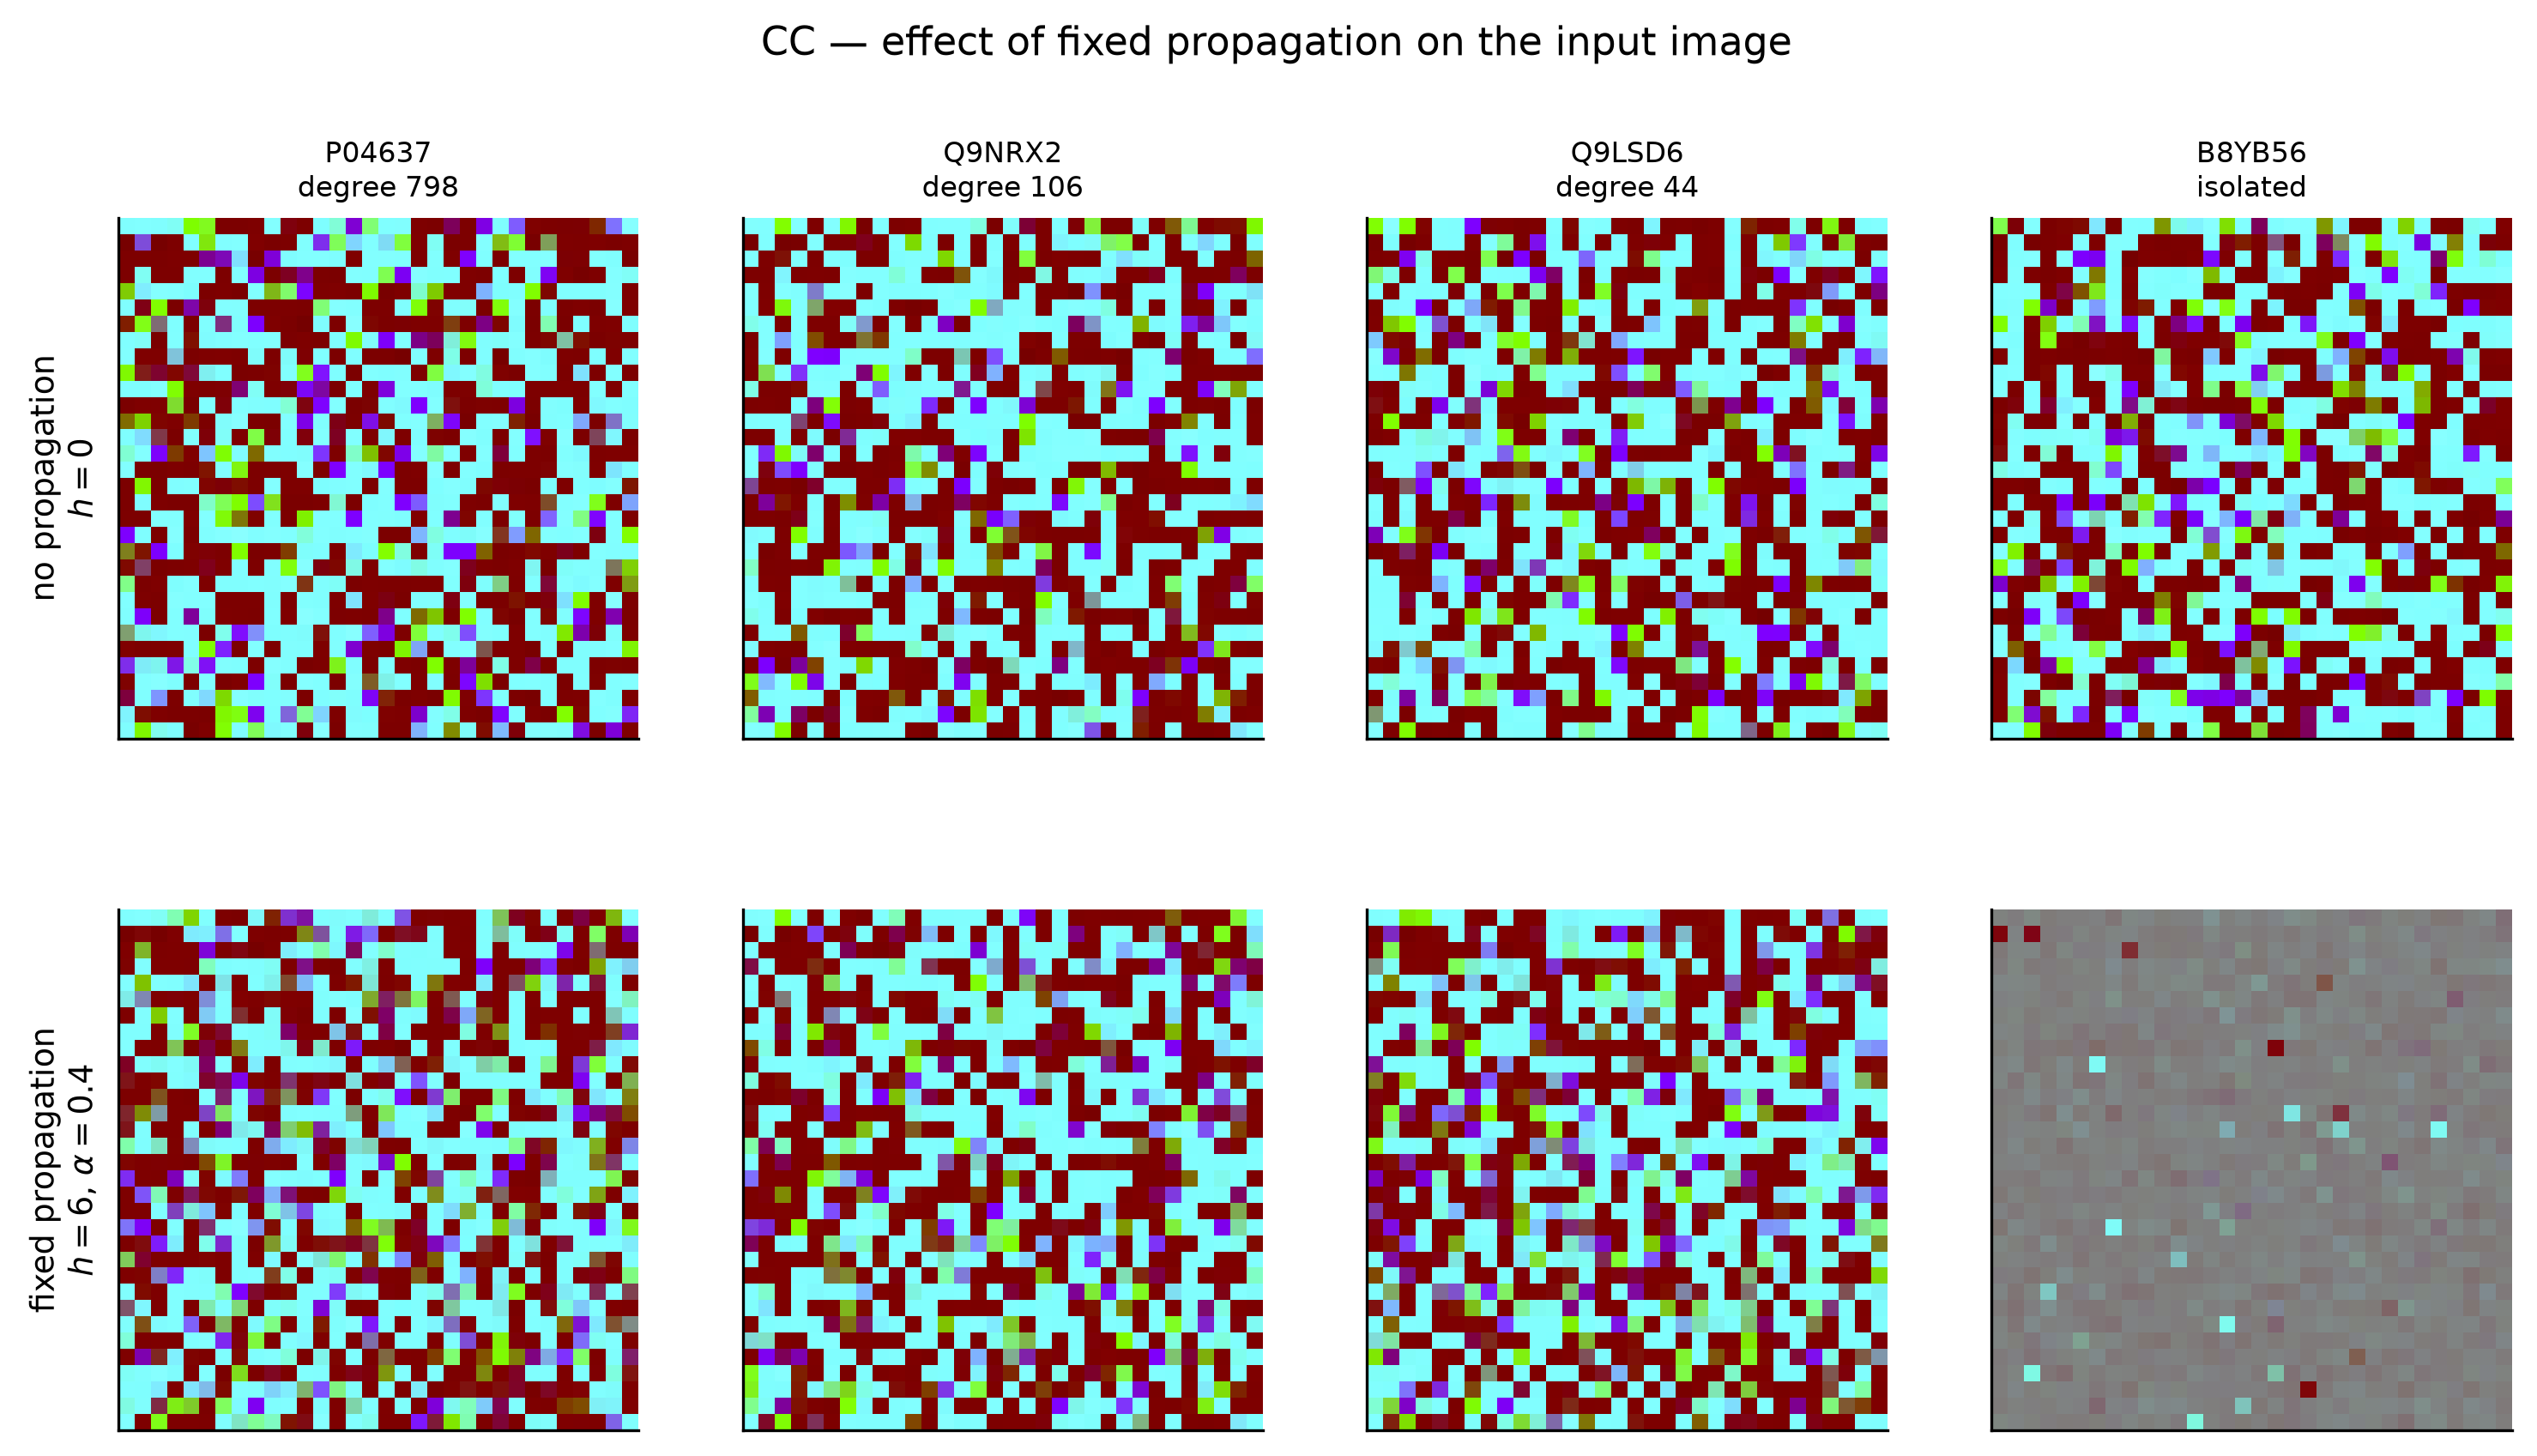
\includegraphics[width=\textwidth]{cap5/fig_5_08_fixed_propagation.png}
  \caption[Effect of the fixed propagation across the degree range]{Effect of the fixed propagation
  of Equation~\eqref{eq:met_recorrencia} on four Cellular Component proteins of decreasing degree,
  rendered through the mapping of Section~\ref{sec:met_head_visao}. Top row: $T = 0$, where the
  operator is the identity and every protein shows its own sequence representation. Bottom row:
  $T = 6$ and $\alpha = 0.4$. The three connected proteins retain their structure while acquiring
  their neighborhood; the isolated protein, whose row of $P^{\top}$ is empty, retains
  $\alpha^{T}\mathbf{H}^{(0)}$ and is driven toward a uniform array.}
  \label{fig:met_fixa}
\end{figure}

\subsubsection{Learned Propagation}
\label{sec:met_gnn}

The second route makes the aggregation parametric and optimizes it jointly with the prediction head.
Two convolution operators are used, both applied over the same sparse graph of
Section~\ref{sec:met_grafo}. In both cases, self-loops are added to the adjacency before
normalization, so that the update of a protein always includes a term in its own previous
representation; this is the standard formulation of both operators, and it is the mechanism by which
a protein's own signal survives the aggregation. It also means that in this route an isolated
protein is never mixed with the representation of any other protein, in contrast with the
$\alpha^{T}$ scaling noted in Section~\ref{sec:met_fixa}. Its representation is not passed through
unchanged, however: it still undergoes the learned linear transformations, the biases and the
nonlinearities of every layer.

The graph convolutional operator consumes the weighted matrix $W$ of
Section~\ref{sec:met_grafo} rather than a binary adjacency. Writing
\begin{equation}
  \tilde{W} \;=\; W + I,
  \qquad
  \tilde{D}_{ii} \;=\; \sum_{j} \tilde{W}_{ij},
  \label{eq:met_gcn_norm}
\end{equation}
\noindent for the self-loop-augmented weight matrix and its degree matrix, the layer applies a symmetric
normalization followed by a linear transformation and a pointwise nonlinearity $\phi$~\cite{kipf2017semi}:
\begin{equation}
  \mathbf{H}^{(\ell+1)} \;=\;
  \phi\!\left( \tilde{D}^{-1/2}\,\tilde{W}\,\tilde{D}^{-1/2}\;\mathbf{H}^{(\ell)}\;\Theta^{(\ell)} \right).
  \label{eq:met_gcn}
\end{equation}

The added self-loop carries unit weight, which is the default of the implementation used, so a
protein's own attribute enters its update with a weight of one against confidences in
$[0.400,\,0.999]$ for its neighbors. The interaction confidence therefore enters as the scalar
weight
of its edge: the operator takes the STRING score as given and uses it directly to modulate the
aggregation.

The graph attention operator instead estimates the aggregation weights. Self-loops are added to the
edge set before the attention is computed, so that the neighborhood of $i$ is
$\mathcal{N}(i) \cup \{i\}$; the attribute assigned to each added self-loop is the mean of the
attributes of the edges incident to that vertex, which is the default of the implementation used,
and
an isolated vertex therefore receives a self-loop whose attribute is null. For each ordered pair of
adjacent proteins an unnormalized score is computed from the transformed representations of the two
endpoints together with the edge attribute, and the scores are normalized over that neighborhood
\cite{velickovic2018graph}:
\begin{equation}
  e_{ij} \;=\; \operatorname{LeakyReLU}\!\left(
      \mathbf{q}^{\top}
      \left[\, \Theta \mathbf{h}_i \;\big\|\; \Theta \mathbf{h}_j \;\big\|\; \Theta_e\, w_{ij} \,\right]
    \right),
  \qquad
  a_{ij} \;=\; \frac{\exp(e_{ij})}
  {\displaystyle\sum_{k \,\in\, \mathcal{N}(i) \cup \{i\}} \exp(e_{ik})},
  \label{eq:met_gat}
\end{equation}
\noindent where $\Theta$ is the transformation shared by the two endpoints,
$\Theta_e$ lifts the scalar edge attribute to the same width that $\Theta$ produces,
$\mathbf{q}$
is the learned attention vector, and the rectifier has a negative slope of $0.2$.
Attention is
computed with four parallel heads in the hidden layers; each head emits one quarter of the hidden
width and the four outputs are concatenated, so the width of a hidden layer is the same as it would
be with a single head. The output layer uses one head and does not concatenate.

Three properties of this route are stated here because they are not visible in
Equations~\eqref{eq:met_gcn} and~\eqref{eq:met_gat}. First, the convolution stack does not emit the
term scores. Its last layer produces a latent representation
\begin{equation}
  \mathbf{g}_i \;\in\; \mathbb{R}^{1024},
  \label{eq:met_gnn_emb}
\end{equation}
\noindent which is consumed by one of the prediction heads of Section~\ref{sec:met_heads}, whose final linear
layer emits one score per retained Gene Ontology term. Second, the rectified activation and the
dropout are applied between consecutive layers only, so $\mathbf{g}_i$ is the output of the last
convolution before any activation and before any dropout. It is read from the checkpoint selected by
the early-stopping criterion, with the model in evaluation mode and without gradients, and it is
this
representation that Section~\ref{sec:met_early} caches and reuses. Third, the edge attribute
$w_{ij}$
entering
Equation~\eqref{eq:met_gat} is the deduplicated combined score on its original scale, not the
column-normalized weight of Equation~\eqref{eq:met_P}, which is consumed by the fixed operator
alone. The distinction is deliberate, since the attention mechanism normalizes over each
neighborhood through its own softmax and a pre-normalized attribute would duplicate that operation;
it is recorded because it means the two propagation routes do not consume an identical edge object.

Both operators are applied in a full-graph forward pass: under the exact propagation adopted in this
implementation the graph operator is evaluated over all $|\mathcal{V}|$ vertices before the rows of
the current loss mini-batch are selected by Equation~\eqref{eq:met_mascara}. This follows from the
combination of exact propagation with a mini-batch loss, and not from the problem itself:
full-batch optimization and neighborhood sampling of the kind introduced with GraphSAGE
\cite{hamilton2017graphsage} are alternatives that were not evaluated here. It is also why the
learned route recomputes the propagation at every optimization step, whereas the fixed operator is
computed once per experiment; the measured cost is reported in Appendix~\ref{ape:implementacao}.

\subsubsection{Depth and Smoothing}
\label{sec:met_contraste}

Both routes inherit a limitation of the message-passing paradigm. Each additional step enlarges the
receptive field of a protein by one hop, which is the intended effect, but it also moves every
representation closer to a weighted average over its expanding neighborhood. In the limit, on a
connected component, repeated averaging drives all representations toward a common vector determined
by the graph rather than by the proteins, and the individual signal that the sequence representation
provides is progressively erased (a phenomenon usually termed oversmoothing)
\cite{li2018deeper, oono2020graph}. The number of propagation steps is therefore not a quantity to
be maximized: it trades the benefit of a wider neighborhood against the loss of node-level
discriminability, and the balance depends on the density of the graph.

The two routes respond to this trade-off differently. In Equation~\eqref{eq:met_recorrencia} the
retention coefficient $\alpha$ is an explicit brake: a fraction $\alpha$ of the representation
produced by the previous step survives into the next, so the operator interpolates between the
identity and pure diffusion, and depth can be increased without the representation collapsing as
quickly as unmixed
averaging would imply. In the learned route the corresponding role is played by the self-loop term
inside Equations~\eqref{eq:met_gcn}--\eqref{eq:met_gat}, whose weight is fixed by the normalization
rather than chosen; depth there is limited to a small number of layers, which is the usual practice
for these operators.

Beyond depth, three differences separate the routes. The first is the inductive bias: the fixed
operator takes the STRING confidence as a reliable weight and performs a convex combination
prescribed by it, whereas the attention operator treats the confidence as evidence to be
re-estimated during training. The second is the parameter count: propagation contributes none in the
fixed route and a full set of transformation and attention parameters in the learned one. The third
is cost, and it follows directly from the previous part: the fixed operator runs once per
experiment and is cached, while the learned operators recompute the full-graph propagation at every
optimization step.

\subsection{Prediction Head}
\label{sec:met_heads}

Two heads consume the representation produced by either propagation route. The first is the default
vector head; the second reuses the convolutional backbones already introduced in
Section~\ref{sec:met_gen1_img}.

\subsubsection{Vector Head}
\label{sec:met_head_vetor}

The default head is a multilayer perceptron. Each hidden block consists of a linear layer, batch
normalization, a rectified linear activation and dropout, and the block is repeated according to the
configured widths; a final linear layer emits $|\mathcal{C}|$ values, one per Gene Ontology term of
the ontology being modeled.

The head emits logits and contains no output nonlinearity. The sigmoid that maps a logit to a
per-term probability is applied inside the objective function, in the numerically stable formulation
that combines it with the loss, and again at inference time when probabilities are required. The
distinction determines how the outputs of Section~\ref{sec:met_fusion} are combined: early fusion
operates on representations, before the head, and late fusion operates on probabilities, after the
sigmoid. The learning rate and the early-stopping patience are reported in
Appendix~\ref{ape:implementacao}. These architectural choices were grounded in preliminary
empirical evaluations where different configurations were analyzed. Since this setup yielded the
best average performance across the initially assessed metrics, it was fixed to ensure consistency
throughout the main reported experiments in Chapter~\ref{cap:resultados}.

\subsubsection{Vision Head}
\label{sec:met_head_visao}

An alternative head applies the two backbones of Section~\ref{sec:met_gen1_img}, ResNet-50 and
ConvNeXt-Tiny, to the second generation's representation. The representation vector, propagated or
not, is mapped into an image which is then consumed by the backbone. Let
$\mathbf{z} \in \mathbb{R}^{3072}$ denote that representation, that is, a row of $\mathbf{H}^{(T)}$.
Its coordinates are first clipped to $[-50, 50]$ to limit extreme inputs to the logistic mapping, then mapped by the logistic function, and
the resulting values in $[0,1]$ are partitioned into three blocks of $1024$, each reshaped into a
$32 \times 32$ array that becomes one channel:
\begin{equation}
\begin{split}
  \mathbf{z} \;\in\; \mathbb{R}^{3072} \;&\longmapsto\; \sigma\!\bigl(\operatorname{clip}(\mathbf{z}, -50, 50)\bigr) \;\longmapsto\; X \;\in\; [0,1]^{3 \times 32 \times 32} \\
  X \;&\longmapsto\; \text{backbone}(X) \;\in\; \mathbb{R}^{|\mathcal{C}|}.
\end{split}
\label{eq:met_reshape}
\end{equation}

The tensor $X$ is the input to the backbone; the term logits are the output of the backbone, not of
this mapping. The three-block partition is not arbitrary: it coincides with the three ProtT5 layers
concatenated in Equation~\eqref{eq:met_h0}, so the first channel corresponds to layer $24$, the
second to layer $23$ and the third to layer $22$. When the input representation is
$1024$-dimensional, a single $32 \times 32$ channel is produced and replicated three times. The
mapping therefore admits representations of $3072$ or $1024$ dimensions only.
Figure~\ref{fig:met_reshape} illustrates the mapping.

\begin{figure}[!htb]
  \centering
  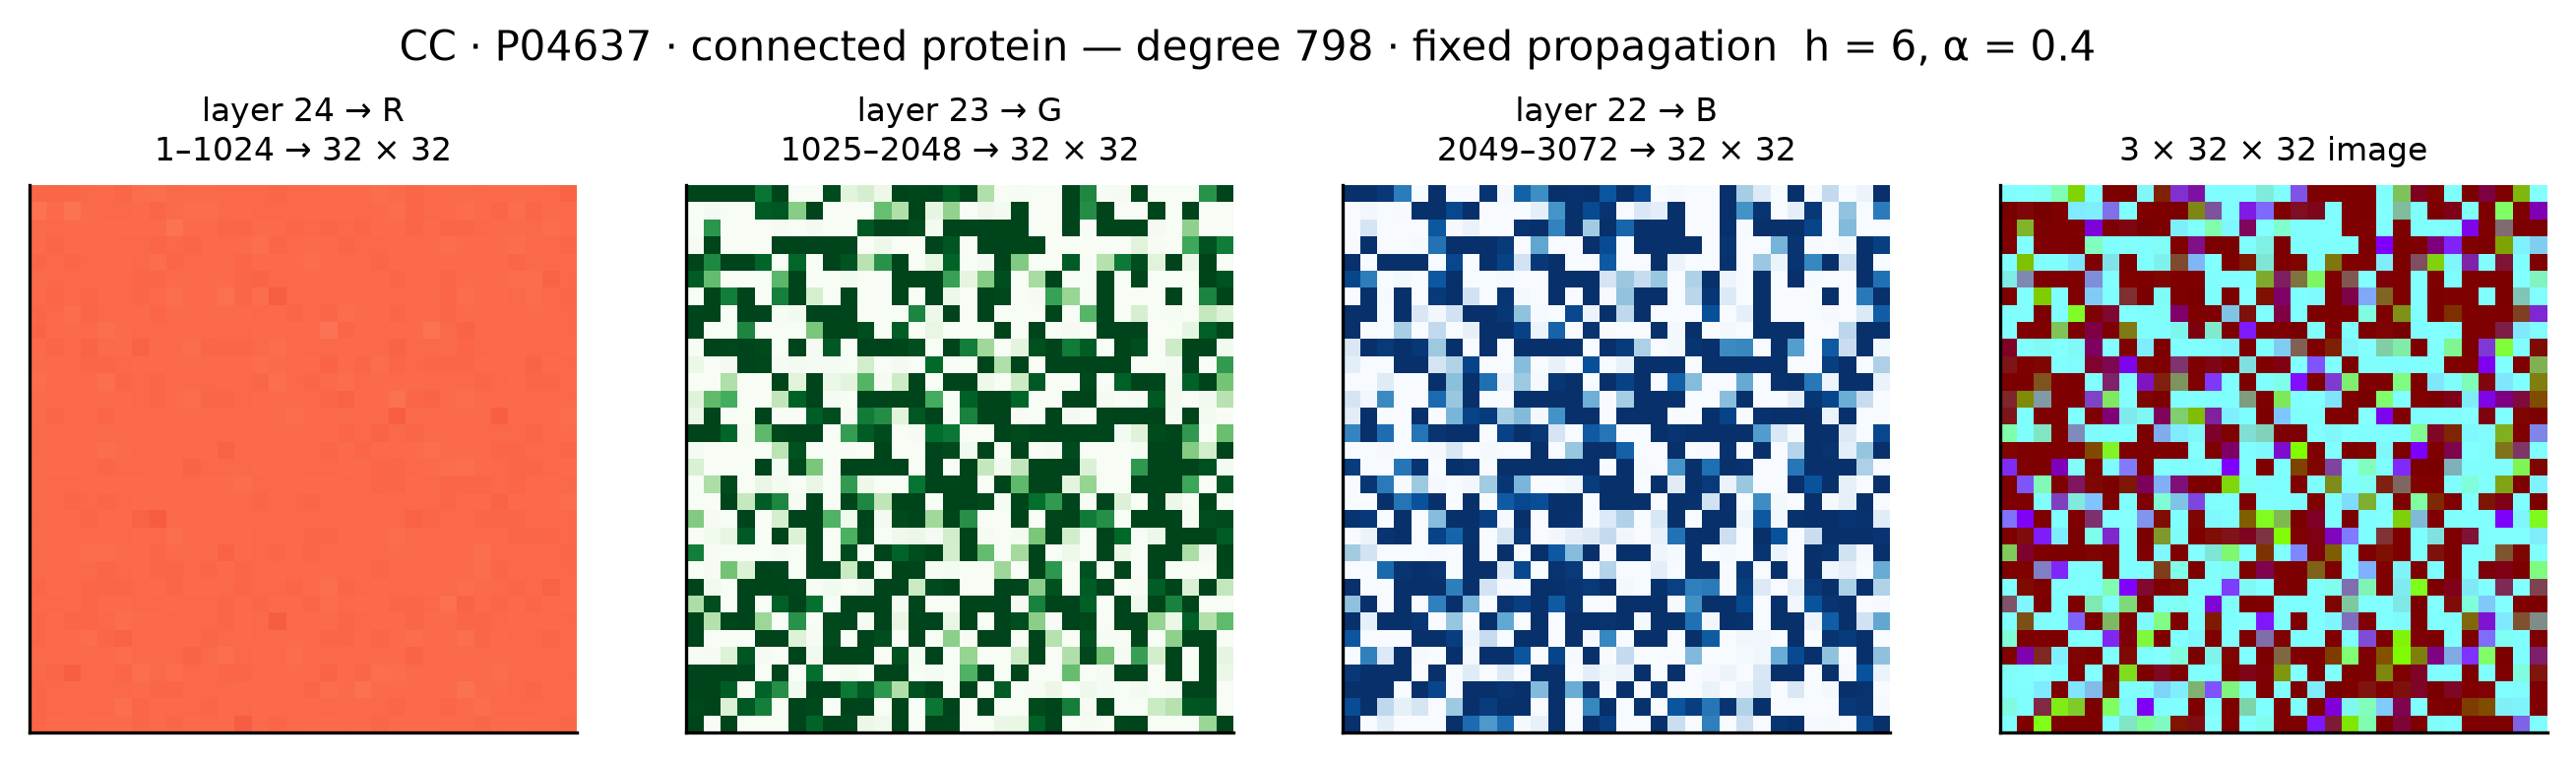
\includegraphics[width=\textwidth]{cap5/fig_5_09_reshape_to_image.png}
  \caption[Mapping the representation into an image]{Mapping of the representation into the input of
  the vision head, following Equation~\eqref{eq:met_reshape}, for a Cellular Component protein of
  degree $798$ after fixed propagation with $T = 6$ and $\alpha = 0.4$. The $3072$-dimensional
  vector is clipped, passed through the logistic function and partitioned into three blocks of
  $1024$, one per ProtT5 layer in the order of Equation~\eqref{eq:met_h0}; each block is reshaped
  into a $32 \times 32$ channel, and the three are stacked into the image consumed by the backbone.}
  \label{fig:met_reshape}
\end{figure}

No image is ever written to disk. The array of Equation~\eqref{eq:met_reshape} is constructed inside
the forward pass, consumed by the backbone in the same call, and discarded; there is no image
dataset associated with this head. It is also not resized: the $32 \times 32$ tensor enters the
backbone at that resolution, well below the input size the pretrained weights were fitted on, so the
spatial extent reaching the deeper stages is small and the transfer is correspondingly weaker than in the first-generation route, whose inputs are constructed directly at $224 \times 224$ from the pooled interaction profile. The head substitution and the unfreezing
described in Section~\ref{sec:met_gen1_img} apply here unchanged. The reshaping is a positional
mapping without geometric meaning
(adjacent coordinates of $\mathbf{z}$ become adjacent pixels only due to the ordering of the embedding
dimensions), and the same caveat raised for the one-dimensional convolution in
Section~\ref{sec:met_gen1_vetor} applies here.

% =====================================================================
\section{Objective Functions}
\label{sec:met_loss}

\paragraph{Binary Cross-Entropy.} The reference objective for multi-label classification treats each
term as an independent binary decision. For a protein with target vector $\mathbf{y}$ and predicted
logits $\mathbf{z}$,
\begin{equation}
  \mathcal{L}_{\text{BCE}} \;=\; -\frac{1}{|\mathcal{C}|}
  \sum_{c \,\in\, \mathcal{C}}
  \Bigl[\, y_c \log \sigma(z_c) \;+\; (1 - y_c)\log\bigl(1 - \sigma(z_c)\bigr) \,\Bigr].
  \label{eq:met_bce}
\end{equation}

Its assumption of independence among terms is violated here, since the label space is a
directed acyclic graph in which the presence of a term implies the presence of all its ancestors,
but it remains the standard against which alternative objectives are read, and it is the objective
under which one of the comparative methods is evaluated. No class rebalancing (neither resampling
nor per-term weighting of Equation~\eqref{eq:met_bce}) is applied; the imbalance of the label
space is left to be handled by the objective below.

\paragraph{The Multi-Label Categorical Cross-Entropy.} The second formulation abandons the per-term
decomposition and treats the problem as a separation between the positive and the negative sets,
with the decision threshold fixed at zero. Writing $\mathcal{P}$ and $\mathcal{N}^{-}$ for the sets of
positive and negative terms of a protein,
\begin{equation}
  \mathcal{L}_{\text{ZLPR}} \;=\;
  \log\!\left(1 + \sum_{c \,\in\, \mathcal{P}} e^{-z_c}\right)
  \;+\;
  \log\!\left(1 + \sum_{c \,\in\, \mathcal{N}^{-}} e^{z_c}\right),
  \label{eq:met_zlpr}
\end{equation}
\noindent which penalizes any positive term scored below zero and any negative term scored above it, with the
log-sum-exp form providing a smooth surrogate for the maximum~\cite{su2022zlpr}. Unlike in
Equation~\eqref{eq:met_bce}, the number of positive terms of a protein does not enter as a
normalizing constant, so proteins with few annotations are not down-weighted relative to
densely annotated ones. This objective is presented here because it is a component of the composite
objective defined below rather than an alternative to it, and it is not evaluated on its own in this
work.

\paragraph{The Composite Objective.} The objective adopted for the proposed models is the
protein-centric composite loss introduced by InterLabelGO+~\cite{liu2024interlabelgo} and inherited
through the sequence-only line reviewed in Chapter~\ref{cap:trabalhos}, where it is referred to as \textsc{ProteinLoss}. It multiplies Equation~\eqref{eq:met_zlpr} by two factors derived from weighted
$F_1$ agreement, one computed across Gene Ontology terms and one across proteins within the batch:
\begin{equation}
  \mathcal{L}_{\text{prot}} \;=\; \mathcal{L}_{\text{ZLPR}} \;\cdot\;
  \bigl(1 - \mathrm{wF}_1^{\text{GO}}\bigr) \;\cdot\;
  \bigl(1 - \mathrm{wF}_1^{\text{prot}}\bigr),
  \label{eq:met_proteinloss}
\end{equation}
\noindent where both factors are evaluated on the probabilities $\hat{p}_{ic} = \sigma(z_{ic})$, whereas
$\mathcal{L}_{\text{ZLPR}}$ is evaluated on the logits.

The two factors share one definition and differ only in the axis along which they are reduced. For a
batch $\mathcal{B}$ of proteins, a set $\mathcal{C}$ of terms and the information content
$\mathrm{IC}(c)$ of Chapter~\ref{cap:materiais}, write the soft weighted counts along an axis
$\mathcal{S}$ as
\begin{equation}
  \begin{aligned}
    \mathrm{tp}(\mathcal{S}) &= \sum_{(i,c) \in \mathcal{S}} \mathrm{IC}(c)\, y_{ic}\, \hat{p}_{ic}, \\
    \mathrm{fp}(\mathcal{S}) &= \sum_{(i,c) \in \mathcal{S}} \mathrm{IC}(c)\, (1 - y_{ic})\, \hat{p}_{ic}, \\
    \mathrm{fn}(\mathcal{S}) &= \sum_{(i,c) \in \mathcal{S}} \mathrm{IC}(c)\, y_{ic}\, (1 - \hat{p}_{ic}).
  \end{aligned}
  \label{eq:met_softcounts}
\end{equation}

No threshold is applied: the counts are soft, the predicted probability entering in place of a
binary
decision. The corresponding soft precision, recall and $F_1$ are
\begin{equation}
  \begin{aligned}
    \mathrm{pr}(\mathcal{S}) &= \frac{\mathrm{tp}(\mathcal{S})}{\mathrm{tp}(\mathcal{S}) + \mathrm{fp}(\mathcal{S}) + \epsilon},
    \qquad
    \mathrm{rc}(\mathcal{S}) = \frac{\mathrm{tp}(\mathcal{S})}{\mathrm{tp}(\mathcal{S}) + \mathrm{fn}(\mathcal{S}) + \epsilon}, \\[4pt]
    F_1(\mathcal{S}) &= \frac{2\, \mathrm{pr}(\mathcal{S})\, \mathrm{rc}(\mathcal{S})}{\mathrm{pr}(\mathcal{S}) + \mathrm{rc}(\mathcal{S}) + \epsilon},
  \end{aligned}
  \label{eq:met_softf1}
\end{equation}
\noindent with $\epsilon = 10^{-16}$ guarding every denominator, so a slice whose three counts vanish yields
$F_1 = 0$ rather than an undefined value; any residual non-finite entry is set to zero before the
reduction. The two factors then differ only in how the index set is sliced. The term-centric factor
fixes a term and reduces over the proteins of the batch, and the protein-centric factor fixes a
protein and reduces over the terms:
\begin{equation}
  \mathrm{wF}_1^{\text{GO}} = \frac{1}{|\mathcal{C}|} \sum_{c \in \mathcal{C}} F_1\bigl(\mathcal{B} \times \{c\}\bigr),
  \qquad
  \mathrm{wF}_1^{\text{prot}} = \frac{1}{|\mathcal{B}|} \sum_{i \in \mathcal{B}} F_1\bigl(\{i\} \times \mathcal{C}\bigr).
  \label{eq:met_wf1_axes}
\end{equation}

Two consequences of Equation~\eqref{eq:met_wf1_axes} are worth stating. The term-centric factor is
estimated along the batch dimension, so the number of proteins in a batch enters the definition of
the objective and not only the optimization; the batch size was held fixed for that reason. And
because a term contributes the same weight $\mathrm{IC}(c)$ to its numerator and to its denominator
within a slice of fixed $c$, the information content cancels in $\mathrm{wF}_1^{\text{GO}}$ but not
in $\mathrm{wF}_1^{\text{prot}}$, where the weight varies across the terms being summed.

The rationale for the composite form is to bring the training signal closer in structure to the
evaluation criterion. The metrics of Chapter~\ref{cap:materiais} are built on $F_1$ agreement
between
a predicted and a true annotation set, a quantity that a per-term likelihood does not directly
optimize; the two multiplicative factors of Equation~\eqref{eq:met_proteinloss} attenuate the loss
as
that agreement improves, along the term axis and along the protein axis respectively. The ablation
that isolates the contribution of Equation~\eqref{eq:met_proteinloss} relative to
Equation~\eqref{eq:met_bce} is reported in Chapter~\ref{cap:resultados}.

% =====================================================================
\section{Fusion}
\label{sec:met_fusion}

The two propagation routes of Section~\ref{sec:met_prop}, the fixed operator of
Equation~\eqref{eq:met_recorrencia} and the parametric graph convolutions of
Section~\ref{sec:met_gnn}, produce representations of the same proteins from the same sequence
attributes and the same graph, but under different assumptions about how the interaction confidence
should be used. Rather than selecting between them, this work combines them. There are exactly two
points at which the combination can occur: before the prediction head, on the representations, or
after it, on the probabilities.

The two options are mutually exclusive routes to the same end, not complementary stages, and both
consume the same two sources. Either the representation produced by the fixed operator is joined
with the representation produced by the graph convolution and a single head is trained on the
result, which is early fusion, or each route is trained to convergence with its own head and the two
sets of probabilities are combined, which is late fusion. What differs is the level at which the two
sources meet, and consequently whether a head is given the opportunity to learn how to weigh them.
No model is shared between the two routes, and Chapter~\ref{cap:resultados} compares them directly.
Figure~\ref{fig:met_fusao} places them side by side.

\begin{figure}[!htb]
  \centering
  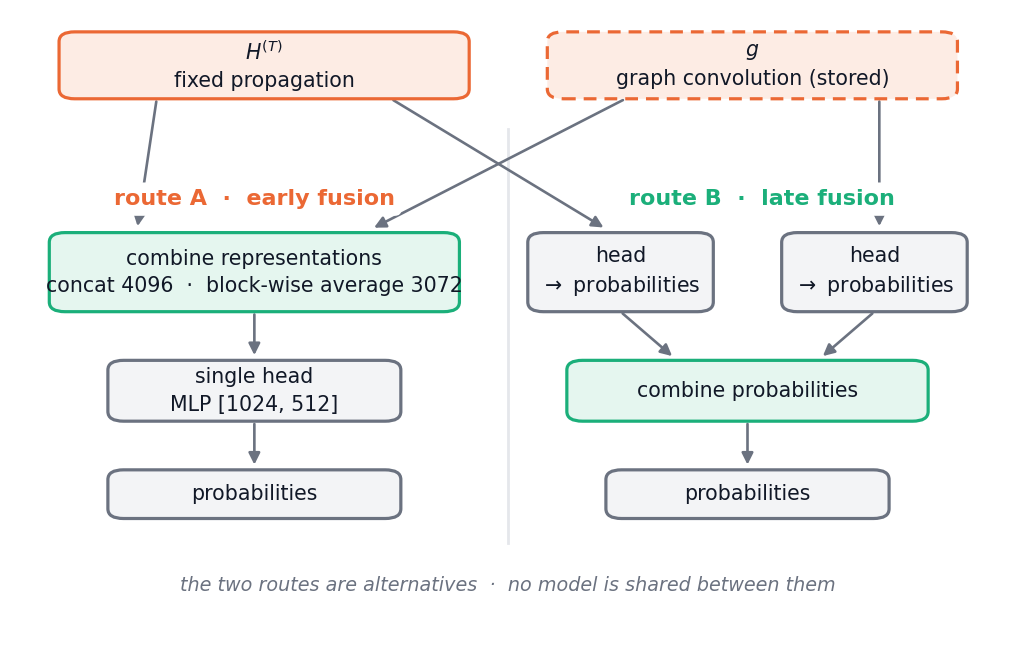
\includegraphics[width=0.8\textwidth]{cap5/fig_5_10_early_late_fusion.png}
  \caption[Early and late fusion]{The two fusion routes. Both consume the same two sources, the
  representation $\mathbf{H}^{(T)}$ produced by the fixed operator of
  Equation~\eqref{eq:met_recorrencia} and the stored representation $\mathbf{g}$ produced by the
  graph convolution, and they differ only in the level at which the two meet. Route~A combines the
  representations and trains a single head on the result. Route~B trains a head on each
  representation separately and combines the resulting probabilities. The routes are alternatives:
  no model is shared between them.}
  \label{fig:met_fusao}
\end{figure}

\subsection{Early Fusion}
\label{sec:met_early}

Early fusion combines the two representations before the prediction head, so that a single
head is trained on the combined representation. The representation produced by the fixed operator of
Equation~\eqref{eq:met_recorrencia} is joined with the $1024$-dimensional representation
$\mathbf{g}_i$ of Equation~\eqref{eq:met_gnn_emb}. This route therefore performs feature-level
fusion
with a pretrained and frozen graph branch: the convolutional representation is computed from a
previously selected checkpoint and cached, and only the downstream fusion head is optimized during
the fusion experiment.

Two combination operators are considered. The concatenative variant appends the two vectors,
\begin{equation}
  \mathbf{H}^{\text{concat}}_i \;=\;
  \left[\, \mathbf{H}^{(T)}_i \;\big\|\; \mathbf{g}_i \,\right] \;\in\; \mathbb{R}^{4096},
  \label{eq:met_concat}
\end{equation}
\noindent where $\mathbf{g}_i$ is the convolutional representation of protein $i$, and leaves to the head the
task of deciding how much of each source to use. The additive variant instead keeps the
dimensionality of the sequence representation, exploiting the block structure of
Equation~\eqref{eq:met_h0}. Writing the propagated representation as
$\mathbf{H}^{(T)}_i = [\, \mathbf{h}^{(24)}_i \,\|\, \mathbf{h}^{(23)}_i \,\|\, \mathbf{h}^{(22)}_i \,]$,
the convolutional representation is averaged into each of the three $1024$-dimensional layer blocks,
\begin{equation}
  \mathbf{H}^{\text{add}}_i \;=\;
  \frac{1}{2}\left[\,
    \bigl(\mathbf{h}^{(24)}_i + \mathbf{g}_i\bigr) \;\big\|\;
    \bigl(\mathbf{h}^{(23)}_i + \mathbf{g}_i\bigr) \;\big\|\;
    \bigl(\mathbf{h}^{(22)}_i + \mathbf{g}_i\bigr)
  \,\right] \;\in\; \mathbb{R}^{3072}.
  \label{eq:met_add}
\end{equation}

The concatenative variant imposes no constraint on the two dimensionalities, whereas the additive one
requires them to be compatible and presupposes that the two representations live in comparable
spaces, an assumption the concatenative variant avoids. The choice also determines which prediction
head can consume the result. Equation~\eqref{eq:met_concat} produces $4096$ dimensions, which the
vision head of Section~\ref{sec:met_head_visao} does not admit, so the concatenative variant is
combined exclusively with the vector head; Equation~\eqref{eq:met_add} preserves the $3072$
dimensions of the sequence representation and is admitted by both.

The head that consumes the fused representation is held fixed across the whole family, at two hidden
layers of width $1024$ and $512$, so that a difference between the two fusion operators cannot be
attributed to a difference in head capacity.

\subsection{Late Fusion}
\label{sec:met_late}

Late fusion combines the same two sources on the output side. Each route is trained separately and
to convergence with its own prediction head, and the two resulting probability matrices are combined
without retraining either model. Because the combination happens after the sigmoid, no head is
exposed to both representations, so no parameter learns how much of each source to trust and the
combination rule must supply that. In exchange, each route converges under its own optimization
dynamics rather than a shared one, and the combination itself requires no training.

Let $\hat{\mathbf{Y}}_{\text{fix}}$ and $\hat{\mathbf{Y}}_{\text{gnn}}$ denote the predicted
probability matrices of dimension $|\mathcal{V}_{\text{eval}}| \times |\mathcal{C}|$ produced by the
fixed propagation model and by the graph convolution model respectively, where
$\mathcal{V}_{\text{eval}}$ is the partition being scored. Seven families of combination rule are
evaluated to compute the fused matrix $\hat{\mathbf{Y}}_{\text{ens}}$, presented below in six
groups.
Because the stacking family is instantiated with five different meta-classifiers, the experimental
comparison contains eleven individual variants.

\paragraph{1. Linear combination.} The probabilities are combined through a scalar mixing
coefficient $\gamma \in [0,1]$ that governs the contribution of each model:
\begin{equation}
  \hat{\mathbf{Y}}_{\text{ens}} \;=\; \gamma\, \hat{\mathbf{Y}}_{\text{fix}}
  \;+\; (1 - \gamma)\, \hat{\mathbf{Y}}_{\text{gnn}}.
  \label{eq:met_ens_linear}
\end{equation}

\paragraph{2. Pointwise minimum and maximum.} These are two distinct rules, in which the fused
probability is the element-wise minimum or the element-wise maximum of the two matrices:
\begin{equation}
  \hat{\mathbf{Y}}_{\text{ens}} \;=\; \min\!\bigl(\hat{\mathbf{Y}}_{\text{fix}},\, \hat{\mathbf{Y}}_{\text{gnn}}\bigr)
  \qquad \text{or} \qquad
  \hat{\mathbf{Y}}_{\text{ens}} \;=\; \max\!\bigl(\hat{\mathbf{Y}}_{\text{fix}},\, \hat{\mathbf{Y}}_{\text{gnn}}\bigr).
  \label{eq:met_ens_minmax}
\end{equation}

\paragraph{3. Term-specific weighting.} This rule assigns a weight $\omega_j$ to each Gene Ontology
term $j$ from its information content $\mathrm{IC}_j$, defined in Chapter~\ref{cap:materiais}:
\begin{equation}
  \omega_j \;=\; \sigma\!\bigl(\kappa_{\mathrm{IC}} \cdot (\mathrm{IC}_j - \mathrm{IC}_{\text{thr}})\bigr),
  \label{eq:met_ens_gj}
\end{equation}
\begin{equation}
  \bigl(\hat{\mathbf{Y}}_{\text{ens}}\bigr)_{i,j} \;=\;
  \omega_j \bigl(\hat{\mathbf{Y}}_{\text{fix}}\bigr)_{i,j}
  \;+\; (1 - \omega_j) \bigl(\hat{\mathbf{Y}}_{\text{gnn}}\bigr)_{i,j},
  \label{eq:met_ens_ic}
\end{equation}
\noindent where $\mathrm{IC}_{\text{thr}}$ is the midpoint of the transition and $\kappa_{\mathrm{IC}}$
controls its steepness. The sign inside the logistic function places $\omega_j > 1/2$ for terms with
$\mathrm{IC}_j > \mathrm{IC}_{\text{thr}}$, so specific terms are weighted toward the fixed
propagation model and frequent terms toward the graph convolution model.

\paragraph{4. Protein-specific weighting.} This rule assigns a weight $\beta_i$ to each protein $i$
from its node degree $d_i$ in the interaction network of Section~\ref{sec:met_grafo}:
\begin{equation}
  \beta_i \;=\; \sigma\!\bigl(\kappa_{\deg} \cdot (d_{\text{thr}} - d_i)\bigr),
  \label{eq:met_ens_beta}
\end{equation}
\begin{equation}
  \bigl(\hat{\mathbf{Y}}_{\text{ens}}\bigr)_{i,j} \;=\;
  \beta_i \bigl(\hat{\mathbf{Y}}_{\text{fix}}\bigr)_{i,j}
  \;+\; (1 - \beta_i) \bigl(\hat{\mathbf{Y}}_{\text{gnn}}\bigr)_{i,j},
  \label{eq:met_ens_degree}
\end{equation}
\noindent where $d_{\text{thr}}$ is the degree threshold and $\kappa_{\deg}$ controls the steepness. The sign
inside the logistic function is inverted with respect to Equation~\eqref{eq:met_ens_gj}, so that
$\beta_i > 1/2$ for $d_i < d_{\text{thr}}$ and $\beta_i < 1/2$ for $d_i > d_{\text{thr}}$. Isolated
and weakly connected proteins are therefore weighted toward the fixed propagation model, and hubs
toward the graph convolution model.

\paragraph{5. Combined weighting.} The two previous weights are blended through a coefficient
$\lambda \in [0,1]$, distinct from the mixing coefficient $\alpha$ of
Equation~\eqref{eq:met_recorrencia}:
\begin{equation}
  \Omega_{i,j} \;=\; \lambda\, \omega_j \;+\; (1 - \lambda)\, \beta_i,
  \label{eq:met_ens_w}
\end{equation}
\begin{equation}
  \bigl(\hat{\mathbf{Y}}_{\text{ens}}\bigr)_{i,j} \;=\;
  \Omega_{i,j} \bigl(\hat{\mathbf{Y}}_{\text{fix}}\bigr)_{i,j}
  \;+\; (1 - \Omega_{i,j}) \bigl(\hat{\mathbf{Y}}_{\text{gnn}}\bigr)_{i,j}.
  \label{eq:met_ens_master}
\end{equation}

Since $\omega_j$ and $\beta_i$ both lie in $[0,1]$, so does $\Omega_{i,j}$, and
Equation~\eqref{eq:met_ens_master} remains a convex combination of the two predictions.

\paragraph{6. Stacking.} The last rule replaces the explicit weighting functions with a
meta-classifier fitted offline. For a protein $i$ and a term $j$, a feature vector is built from the
two predictions, the information content of the term and the logarithm of the protein degree:
\begin{equation}
  \mathbf{x}_{i,j} \;=\;
  \left[\, \bigl(\hat{\mathbf{Y}}_{\text{fix}}\bigr)_{i,j} ,\;\;
           \bigl(\hat{\mathbf{Y}}_{\text{gnn}}\bigr)_{i,j} ,\;\;
           \mathrm{IC}_j ,\;\;
           \log(d_i + 1) \,\right].
  \label{eq:met_ens_stack}
\end{equation}

Five meta-classifiers are fitted to map $\mathbf{x}_{i,j}$ to the binary ground-truth label
$y_{i,j}$: a decision tree of bounded depth, a logistic regression on standardized features, a
small multilayer perceptron with a single hidden layer and $L_2$ regularization, a random forest of
bounded-depth trees, and a gradient boosting ensemble. The last two extend the single tree to an
averaged and to a boosted ensemble over the same feature vector, so that the comparison separates
the capacity of the meta-classifier from the information available to it. Both auxiliary
features are observable at prediction time: $\mathrm{IC}_j$ is estimated from the training
annotations and $d_i$ from the network topology, so neither carries an evaluation label. Since the
label matrix is heavily imbalanced, each meta-classifier is fitted on a resampled subset that keeps
every positive example of the training partition and draws negatives by rejection sampling up to
five times that number. The resampling shifts
the scale of the resulting scores, which are therefore used as a ranking rather than as calibrated
probabilities; this is consistent with the evaluation protocol of Chapter~\ref{cap:materiais}, in
which every metric is obtained by sweeping the decision threshold.

The two types of parameter that these rules involve are not selected in the same way. The explicit
coefficients ($\gamma$, $\mathrm{IC}_{\text{thr}}$, $\kappa_{\mathrm{IC}}$, $d_{\text{thr}}$,
$\kappa_{\deg}$ and $\lambda$) are chosen by exhaustive search on the validation partition, over
the grid that Appendix~\ref{ape:fusao} reports together with the selected values. The search is
staged rather than joint: the combined rule sweeps $\lambda$ alone, with the four coefficients of
Equations~\eqref{eq:met_ens_gj} to~\eqref{eq:met_ens_degree} frozen at the values that won the
term-specific and the protein-specific rules in that ontology. The meta-classifiers involve
parameters of a second kind. Their architectural and regularization settings are fixed a priori and
are not searched, as Appendix~\ref{ape:fusao} records; their trainable weights are fitted from the
training labels, and therefore from in-sample base-model predictions, which preserves the validation
and the test partitions but may make the meta-classifier overly adapted to the training behavior of
the base models.



% =====================================================================
\section{Experimental Design}
\label{sec:met_design}

\subsection{The Search Space}
\label{sec:met_espaco}

The experiments vary seven factors: the ontology, the edge deduplication rule of
Equation~\eqref{eq:met_dedup}, the number of propagation steps $T$, the mixing coefficient $\alpha$
of Equation~\eqref{eq:met_recorrencia}, the propagation route, the prediction head, and the fusion
strategy. A further set of factors is held fixed by decision rather than explored, so that
differences between configurations remain attributable: the random seed, the dropout rate, the
hidden widths of the fusion head, and the number of data-loading workers. The values are listed in
Appendix~\ref{ape:implementacao}.

The confidence threshold is a configurable parameter in the graph construction. However, since the
combined scores in the inherited interaction file are strictly confined to the $[0.400,\, 0.999]$
interval, the chosen threshold value does not remove any edges, leaving threshold ablation for future work. All
configurations compared in Chapter~\ref{cap:resultados} therefore run on graphs of identical
topology.

\subsection{Selection Funnel and Stored Artifacts}
\label{sec:met_funil}

Selection proceeds as a funnel. Each stage compares a family of configurations on the validation
partition, eliminates the candidates that do not survive it, and passes only its winner to the next
stage; the propagation route is settled before the fusion strategy, and the fusion strategy before
the final confrontation. The test partition is read at a single point, after every choice has been
made.

Each run stores a fixed set of artifacts, so that any reported number can be traced back to the
configuration that produced it: a manifest recording the effective configuration, a summary of the
graph actually built, and the six metrics for the validation partition; the predicted
probability matrices; and the checkpoint of the selected epoch. The naming
convention encodes every factor that changes the result, including the deduplication rule, so that
two runs differing only in edge weighting cannot overwrite one another. The directory layout and the
naming convention are documented in Appendix~\ref{ape:implementacao}.

Two elements of this chapter are proposed rather than inherited: the fixed, non-parametric
propagation of a concatenation of embeddings read from three layers of a protein language model over
the STRING graph, as an alternative to end-to-end graph learning at this scale, and the systematic
combination of that route with a learned one under a single evaluation protocol. The sequence
encoder, the convolution operators, the composite objective, and the metrics are taken from existing
work and were reimplemented under the regime declared in Section~\ref{sec:met_regime}: transductive
node classification over the union of the three partitions, with supervision masked to the training
partition, and with a stricter train-basis construction in the first generation. Selection is
confined to the validation partition and the test partition is read once.
Chapter~\ref{cap:resultados} reports the results.


% =====================================================================
%  CHAPTER 6 — EXPERIMENTS AND RESULTS
%  Requires: booktabs, multirow, xcolor, amsmath, graphicx
%  Standalone version: every table inlined.
% =====================================================================
\chapter{Experiments and Results}
\label{cap:resultados}

This chapter reports the experimental work of the dissertation in the order in which it
was carried out. Section~\ref{sec:expprotocolo} fixes the reading conventions. The two
experimental generations are then presented in turn: Section~\ref{sec:geracao1} covers
the first generation, in which the interaction network is the only input, and
Section~\ref{sec:geracao2} the second, in which ProtT5 embeddings are placed on the same
graph. Section~\ref{sec:vetor_visao} settles a question that cuts across both,
Section~\ref{sec:confronto} confronts the resulting models with the literature, and
Section~\ref{sec:analise} examines cost, connectivity and coverage.

% =====================================================================

\section{Experimental Protocol}
\label{sec:expprotocolo}

Chapters~\ref{cap:materiais} and~\ref{cap:metodologia} define the corpus, the metrics and
the operators, and Appendix~\ref{ape:implementacao} records the hyperparameters, the
hardware and the library versions of every run. This section fixes only what is needed to
read the tables. Every ablation in Sections~\ref{sec:geracao1} to~\ref{sec:vetor_visao} is
read on the validation partition; the test partition appears only in
Section~\ref{sec:confronto} and in the connectivity analysis of Section~\ref{sec:analise},
and no architectural or hyperparameter decision reported here was taken on it. All runs use
a single seed with one run per configuration, so differences below roughly $0.5$ percentage
points of $wF_{\max}$ are treated as ties throughout; this threshold is referred to as the
interpretability floor, and where a decision rests on a margin below it the text says so. Every value follows the metric convention of this work
(ontology root kept, training-derived information content, ancestors propagated) and the five
literature methods were retrained and rescored under it.

Tables that vary a single factor across the three ontologies carry an AVG column, the
arithmetic mean of $wF_{\max}$ over BP, CC and MF. It orders configurations of the same
experiment and nothing more: the information content that weights $wF_{\max}$ is estimated
on the training subset of each ontology separately, so absolute values are not comparable
across ontologies, and the confrontation tables of Section~\ref{sec:confronto} carry no AVG
column for that reason.


% =====================================================================

\section{First Generation}
\label{sec:geracao1}

The first generation asks how far the interaction network can go on its own. The input of
every model in this section is the profile of STRING combined scores of a protein against
the training set; no sequence information enters. The purpose is twofold: to establish the
floor against which the second generation is measured, and to settle three design choices
(the objective, the vector architecture and the vision backbone) before the more
expensive campaign begins.

\subsection{The Naive Baseline}

Table~\ref{tab:naive} reports the term-frequency baseline, which assigns every protein the
training frequency of each GO term and consumes no input at all. It provides a reference level for a predictor that uses no protein-specific input.

\begin{table}[!htb]
  \centering
  \caption{Naive term-frequency baseline ($wF_{\max}$, validation set).}
  \label{tab:naive}
  \begin{tabular}{lcccc}
    \toprule
    Method & BP & CC & MF & AVG \\
    \midrule
    Naive (term frequency) & 39.43 & 47.11 & 44.14 & 43.56 \\
    \bottomrule
  \end{tabular}
\end{table}

This is the simplest method that can be defined for the task: it looks at no protein, at no
sequence and at no edge, and it answers every query with the same ranking of terms. On the
validation partition it nevertheless reaches $39.43$ in BP, $47.11$ in CC and $44.14$ in MF,
for a mean of $43.56$. The level is not negligible, and that is a property of the metric and
of the restricted vocabulary rather than of the method: $wF_{\max}$ weights terms by
information content, and the five hundred most frequent terms of each ontology (the
vocabulary $\mathcal{C}_d$ over which every metric in this chapter is computed) are
precisely the ones a frequency baseline predicts well. Cellular Component is the easiest of
the three to reach this way, at $47.11$, and Biological Process the hardest, at $39.43$.
Table~\ref{tab:naive} therefore serves as a reference baseline: a model that does not exceed these values fails to outperform a predictor that uses no protein-specific input. Every margin reported later in this chapter should therefore be interpreted relative to this reference rather than relative to zero.

\subsection{Objective Function}

Table~\ref{tab:abl_perda} isolates the objective, holding the architecture at an MLP with
\texttt{max} pooling.


\begin{table}[!htb]
  \centering
  \caption{Loss function ablation on the first-generation models ($wF_{\max}$, validation set). Architecture fixed at MLP with \texttt{max} pooling; the only varying factor is the objective. AVG is the arithmetic mean over the three ontologies.}
  \label{tab:abl_perda}
  \begin{tabular}{lcccc}
    \toprule
    Loss Function & BP & CC & MF & AVG \\
    \midrule
    Binary cross-entropy & 31.19 & 42.01 & 37.85 & 37.02 \\
    \textsc{ProteinLoss} & \textBF{34.67} & \textBF{46.08} & \textBF{46.72} & \textBF{42.49} \\
    \bottomrule
  \end{tabular}
\end{table}

\textsc{ProteinLoss} leads binary cross-entropy in all three ontologies, by $3.48$~pp in
BP, $4.07$~pp in CC and $8.87$~pp in MF, for a mean gain of $5.47$~pp. The margin is well
above the interpretability floor everywhere, and its size in MF is the first appearance of
a pattern that recurs throughout the chapter: MF responds more strongly than the other two
ontologies to changes that concern the label space rather than the input. \textsc{ProteinLoss}
is used in every subsequent experiment of both generations.

\subsection{Vector Architecture and Pooling}

Table~\ref{tab:abl_arquitetura} crosses two architectures with three ways of reducing the
score profile.

\begin{table}[!htb]
  \centering
  \caption{Vector architecture and pooling ablation on the first-generation models ($wF_{\max}$, validation set). Loss fixed at \textsc{ProteinLoss}. \texttt{raw} feeds the full score profile against the training set; \texttt{max} and \texttt{avg} pool it beforehand. Best per column in bold, second best underlined.}
  \label{tab:abl_arquitetura}
  \begin{tabular}{llcccc}
    \toprule
    Architecture & Pooling & BP & CC & MF & AVG \\
    \midrule
    \multirow{3}{*}{MLP} & \texttt{max} & \underline{34.67} & \underline{46.08} & \underline{46.72} & \underline{42.49} \\
     & \texttt{avg} & 31.88 & 43.55 & 44.52 & 39.98 \\
     & \texttt{raw} & \textBF{36.37} & \textBF{48.25} & \textBF{48.92} & \textBF{44.51} \\
    \midrule
    \multirow{3}{*}{CNN1D} & \texttt{max} & 32.89 & 44.33 & 46.27 & 41.16 \\
     & \texttt{avg} & 33.33 & 43.93 & 45.09 & 40.78 \\
     & \texttt{raw} & 31.47 & 42.81 & 45.11 & 39.80 \\
    \bottomrule
  \end{tabular}
\end{table}

The MLP over the unreduced profile wins every ontology and leads the best convolutional
configuration by $3.35$~pp on the mean. The ordering of the pooling operators is itself
informative: \texttt{raw} is better than \texttt{max}, which is better than \texttt{avg} for the MLP, with a spread of
$4.53$~pp between the best and the worst. Reducing the profile before the classifier
destroys information the classifier can use, and the one-dimensional convolution (which
imposes an ordering on a vector whose coordinates are training proteins in arbitrary order)
does not recover it. This is the first indication that the inductive bias matters more
than capacity here, a theme Section~\ref{sec:vetor_visao} takes up.

\subsection{Vision Backbone}

The vision route treats the outer absolute-difference image of the score profile as a
two-dimensional input. Table~\ref{tab:abl_backbone} compares two backbones.

\begin{table}[!htb]
  \centering
  \caption{Vision backbone ablation on the first-generation models ($wF_{\max}$, validation set). The input is the outer absolute-difference image of the score profile. Loss fixed at \textsc{ProteinLoss}. Best per column in bold, second best underlined.}
  \label{tab:abl_backbone}
  \begin{tabular}{llcccc}
    \toprule
    Backbone & Pooling & BP & CC & MF & AVG \\
    \midrule
    \multirow{2}{*}{ResNet-50} & \texttt{avg} & 28.94 & 39.78 & \textBF{42.42} & 37.05 \\
     & \texttt{max} & 29.05 & 40.06 & 41.87 & 36.99 \\
    \midrule
    \multirow{2}{*}{ConvNeXt-Tiny} & \texttt{avg} & \textBF{30.40} & \underline{40.38} & \underline{42.08} & \textBF{37.62} \\
     & \texttt{max} & \underline{29.66} & \textBF{40.84} & 41.72 & \underline{37.41} \\
    \bottomrule
  \end{tabular}
\end{table}

The comparison does not resolve cleanly. ConvNeXt-Tiny with \texttt{avg} pooling leads on
the mean, but by $0.57$~pp, and the ordering reverses in MF, where ResNet-50 with the same
pooling is ahead by $0.34$~pp. Neither margin is large enough to decide the question on
this table alone. The backbone adopted for the second generation is ConvNeXt-Tiny, and the argument rests on convergence between independent evidence: the same ordering appeared in the $\mathrm{dedup}=\mathrm{sum}$ campaign reported at VISAPP~\cite{mauhnoom2026graphs}, where the comparison was run under a different deduplication rule. The comparison was not repeated at the second generation: ConvNeXt-Tiny
was carried forward on the strength of this table and of the earlier campaign, and
Section~\ref{sec:vetor_visao} returns to the consequence.

\subsection{What the First Generation Settles}

Three decisions carry forward: \textsc{ProteinLoss} as the objective, the unreduced score
profile with an MLP as the vector route, and ConvNeXt-Tiny as the vision backbone. The
first two rest on margins well clear of the interpretability floor; the third does not. The
performance floor of this generation, a mean $wF_{\max}$ of $44.51$ over the three ontologies for
the best topology-only model, is the number the second generation must improve on. Section~\ref{sec:grau} returns to it, because the topology-only model behaves very
differently from every later model on the proteins the network describes poorly.
% =====================================================================

\section{Second Generation}
\label{sec:geracao2}

The second generation adds ProtT5 embeddings as node attributes on the same STRING network, now
built under the transductive construction of Section~\ref{sec:met_transdutivo} rather than under
the train-basis restriction of the first generation. The question is no longer whether the graph carries signal (the first generation
shows it does) but how much graph is worth using once the sequence is available, and
whether the aggregation should be fixed or learned. The four routes this generation
comprises are the ones named NEXUS-GO in Section~\ref{sec:met_overview}, and are referred
to here as NEXUS-GO/Fixed, NEXUS-GO/GNN, NEXUS-GO/Early and NEXUS-GO/Late wherever the
distinction matters.

\subsection{Fixed Propagation}
\label{sec:fixa}

The fixed operator contextualizes a protein with its neighborhood without training a single
aggregation parameter. This subsection settles its two hyperparameters in order, the
propagation depth first and the mixing coefficient afterwards, on the vector route, and then
repeats both sweeps on the vision route.

\subsubsection{Propagation Depth, Vector Route}
\label{sec:hops}

The fixed operator propagates node attributes without learning: $\mathbf{H}^{(h)} =
\alpha\mathbf{H}^{(h-1)} + (1-\alpha)\mathbf{P}^{\top}\mathbf{H}^{(h-1)}$, applied $T$
times. Table~\ref{tab:sweep_hops_vector} sweeps $T$ with the vector head at
$\alpha = 0.5$, and Figure~\ref{fig:hops_vector} plots it.

\begin{table}[!htb]
  \centering
  \caption{Propagation depth sweep, vector head ($wF_{\max}$, validation set, $\alpha = 0.5$). Best per column in bold, second best underlined.}
  \label{tab:sweep_hops_vector}
  \begin{tabular}{lcccc}
    \toprule
    $T$ & BP & CC & MF & AVG \\
    \midrule
    0 & 53.36 & 65.21 & \textBF{73.18} & \underline{63.92} \\
    1 & \textBF{55.21} & \underline{66.11} & \underline{73.11} & \textBF{64.81} \\
    2 & \underline{54.06} & \textBF{66.13} & 71.18 & 63.79 \\
    3 & 52.12 & 64.71 & 68.61 & 61.81 \\
    4 & 49.85 & 63.03 & 66.70 & 59.86 \\
    5 & 48.17 & 61.58 & 63.81 & 57.85 \\
    6 & 46.45 & 59.91 & 60.75 & 55.70 \\
    7 & 44.72 & 56.86 & 57.93 & 53.17 \\
    8 & 42.08 & 54.07 & 56.81 & 50.99 \\
    9 & 41.81 & 53.64 & 56.76 & 50.74 \\
    10 & 41.61 & 53.33 & 55.58 & 50.17 \\
    \bottomrule
  \end{tabular}
\end{table}

\begin{figure}[!htb]
  \centering
  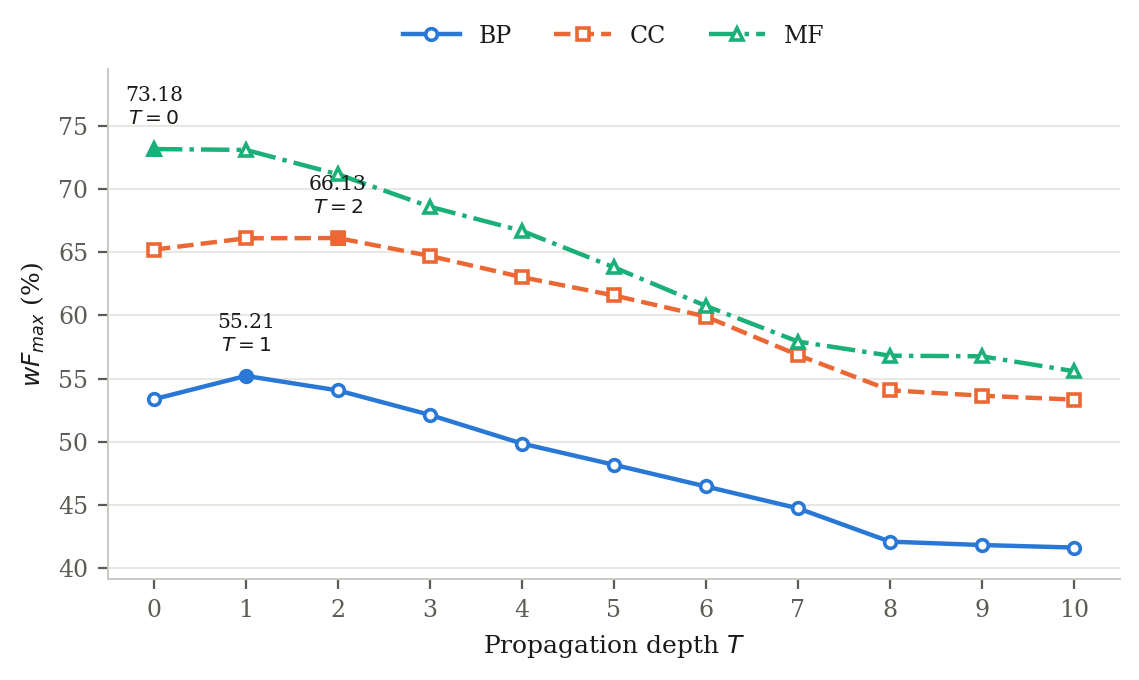
\includegraphics[width=0.92\textwidth]{fig_hops_vetorial}
  \caption{Propagation depth versus $wF_{\max}$ with the vector head (validation set,
  $\alpha = 0.5$). The peak lies at $T=1$ for BP, $T=2$ for CC and $T=0$ for MF.}
  \label{fig:hops_vector}
\end{figure}

The three ontologies do not agree on the optimum. BP peaks at $T=1$, gaining $1.85$~pp
over the graph-free control; CC peaks at $T=2$, gaining $0.92$~pp; MF peaks at $T=0$,
which is to say that no amount of propagation improves it. Beyond the peak the decay is
steep and monotone in all three: $13.60$~pp in BP, $12.80$~pp in CC and $17.60$~pp in MF
between the peak and $T=10$. Whatever the propagation contributes, it contributes it in
one or two steps, and deep diffusion is actively harmful: the representation of a
protein is progressively replaced by the average of an ever wider neighborhood until it
no longer identifies the protein.
In Molecular Function, the
fixed operator has no useful depth: the best configuration is the one in which the
operator is the identity and the graph does not participate in any computation. This is not merely a failure to identify a better depth within the evaluated range; under the corpus, graph, and model configurations considered here, MF does not benefit from fixed propagation. Section~\ref{sec:grau} provides additional evidence about this behavior. %And it also discussed in other literature works that MF has no gains from PPI. (TALVEZ VALE ADCIONAR ESSE COMENTÁRIO).

\subsubsection{Mixing Coefficient, Vector Route}
\label{sec:alpha}

With the depth of each ontology settled, we now evaluate the second hyperparameter of the
operator. The coefficient $\alpha$ controls how much of a node's own representation survives
each step, and it is swept at the depth that the previous sweep selected, so that the two
factors are read one at a time. Table~\ref{tab:sweep_alpha_vector} reports it, and
Figure~\ref{fig:alpha_vector} plots the two ontologies that have a depth to sweep.

\begin{table}[!htb]
  \centering
  \caption{Mixing coefficient sweep, vector head ($wF_{\max}$, validation set) at the best depth of each ontology (BP $T=1$, CC $T=2$, MF $T=0$). \textit{n/a}: inapplicable by construction, since at $T=0$ the propagation operator is the identity and $\alpha$ multiplies nothing. The AVG column averages BP and CC, the two ontologies with a coefficient to sweep. Best per column in bold, second best underlined.}
  \label{tab:sweep_alpha_vector}
  \begin{tabular}{lcccc}
    \toprule
    $\alpha$ & BP & CC & MF & AVG \\
    \midrule
    0.1 & 49.72 & 58.49 & \textit{n/a} & 54.11 \\
    0.2 & 52.69 & 62.26 & \textit{n/a} & 57.48 \\
    0.3 & 53.46 & 63.60 & \textit{n/a} & 58.53 \\
    0.4 & 54.72 & 65.57 & \textit{n/a} & 60.15 \\
    0.5 & \underline{55.21} & 66.13 & 73.18 & 60.67 \\
    0.6 & 55.08 & 65.86 & \textit{n/a} & 60.47 \\
    0.7 & \textBF{55.23} & \underline{66.84} & \textit{n/a} & \textBF{61.04} \\
    0.8 & 54.49 & \textBF{66.94} & \textit{n/a} & \underline{60.72} \\
    0.9 & 53.38 & 66.31 & \textit{n/a} & 59.85 \\
    \bottomrule
  \end{tabular}
\end{table}

\begin{figure}[!htb]
  \centering
  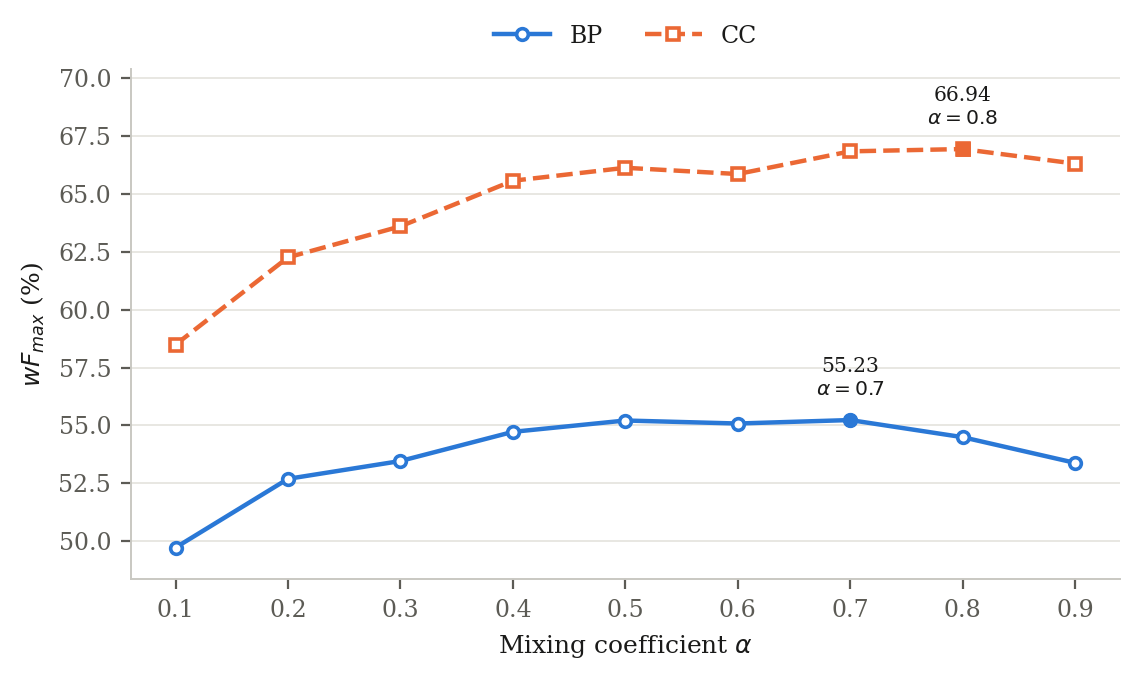
\includegraphics[width=0.92\textwidth]{fig_alpha_vetorial}
  \caption{Mixing coefficient versus $wF_{\max}$ with the vector head (validation set),
  at the best depth of each ontology. MF is omitted: at $T=0$ the coefficient is
  inapplicable.}
  \label{fig:alpha_vector}
\end{figure}


Both ontologies that have a depth to sweep prefer a coefficient in the upper half of the
range, but not the same one: BP peaks at $\alpha = 0.7$ with $55.23$ and CC at
$\alpha = 0.8$ with $66.94$. Neither optimum is sharp, and the disagreement between them
costs little. Reading each ontology against its own best, BP loses at most $0.74$~pp inside
the $0.5$--$0.8$ band, at $\alpha = 0.8$, and CC at most $1.08$~pp, at $\alpha = 0.6$; every
other setting of the band is closer than that to the respective optimum. The AVG column,
which is the only place in the table where one coefficient is asked to serve both
ontologies, peaks at $\alpha = 0.7$ with $61.04$ and places $\alpha = 0.8$ second at
$60.72$. Each ontology is therefore swept and set on its own, as everywhere else in this
chapter, but the setting is a fine adjustment rather than a choice the data forces.
What the two curves agree on is the shape: performance climbs steeply from $\alpha = 0.1$,
flattens across the $0.5$--$0.8$ band and falls at $\alpha = 0.9$. The amplitude across the
whole swept range is substantial, $5.51$~pp in BP and $8.45$~pp in CC between the best and
the worst setting, and it is concentrated at the low end: everything below $\alpha = 0.4$ is
worse than everything above it in CC, and in BP with the single exception of $\alpha = 0.9$. Retention therefore dominates diffusion. Read together with the depth sweep, the two tables
say the same thing from different directions: the graph is useful as a correction to the
node's own representation, not as a replacement for it.

\subsubsection{Vision Route}

Depth and coefficient having been settled for the vector route, the same two sweeps were
repeated with the vision head, so that the choice of prediction head does not remain
confounded with the choice of propagation. Tables~\ref{tab:sweep_hops_vision}
and~\ref{tab:sweep_alpha_vision} mirror the vector tables cell for cell, and
Figures~\ref{fig:hops_vision} and~\ref{fig:alpha_vision} plot them, so the two routes can
be read side by side.

\begin{table}[!htb]
  \centering
  \caption{Propagation depth sweep, vision head ($wF_{\max}$, validation set, $\alpha = 0.5$). Best per column in bold, second best underlined.}
  \label{tab:sweep_hops_vision}
  \begin{tabular}{lcccc}
    \toprule
    $T$ & BP & CC & MF & AVG \\
    \midrule
    0 & 46.33 & 60.13 & \textBF{68.25} & 58.24 \\
    1 & 47.19 & 61.04 & \underline{67.04} & 58.42 \\
    2 & 48.74 & 61.91 & 66.38 & 59.01 \\
    3 & 49.78 & 62.53 & 65.38 & 59.23 \\
    4 & 50.73 & 62.59 & 64.90 & \textBF{59.41} \\
    5 & 51.77 & \underline{62.83} & 63.50 & 59.37 \\
    6 & 51.73 & \textBF{63.06} & 63.34 & \underline{59.38} \\
    7 & \textBF{52.17} & 62.47 & 63.17 & 59.27 \\
    8 & \underline{51.86} & 62.44 & 63.59 & 59.30 \\
    9 & 51.25 & 62.07 & 63.33 & 58.88 \\
    10 & 50.98 & 62.12 & 62.74 & 58.61 \\
    \bottomrule
  \end{tabular}
\end{table}

\begin{table}[!htb]
  \centering
  \caption{Mixing coefficient sweep, vision head ($wF_{\max}$, validation set) at the best depth of each ontology (BP $T=7$, CC $T=6$, MF $T=0$). \textit{n/a}: inapplicable by construction, as in Table~\ref{tab:sweep_alpha_vector}. The AVG column averages BP and CC. Best per column in bold, second best underlined.}
  \label{tab:sweep_alpha_vision}
  \begin{tabular}{lcccc}
    \toprule
    $\alpha$ & BP & CC & MF & AVG \\
    \midrule
    0.1 & 40.66 & 52.44 & \textit{n/a} & 46.55 \\
    0.2 & 40.96 & 52.62 & \textit{n/a} & 46.79 \\
    0.3 & 50.15 & 61.87 & \textit{n/a} & 56.01 \\
    0.4 & 51.06 & 62.14 & \textit{n/a} & 56.60 \\
    0.5 & \textBF{52.17} & \textBF{63.06} & 68.25 & \textBF{57.62} \\
    0.6 & \underline{51.90} & \underline{62.61} & \textit{n/a} & \underline{57.26} \\
    0.7 & 51.02 & 62.40 & \textit{n/a} & 56.71 \\
    0.8 & 49.64 & 61.97 & \textit{n/a} & 55.81 \\
    0.9 & 47.32 & 60.99 & \textit{n/a} & 54.16 \\
    \bottomrule
  \end{tabular}
\end{table}

\begin{figure}[!htb]
  \centering
  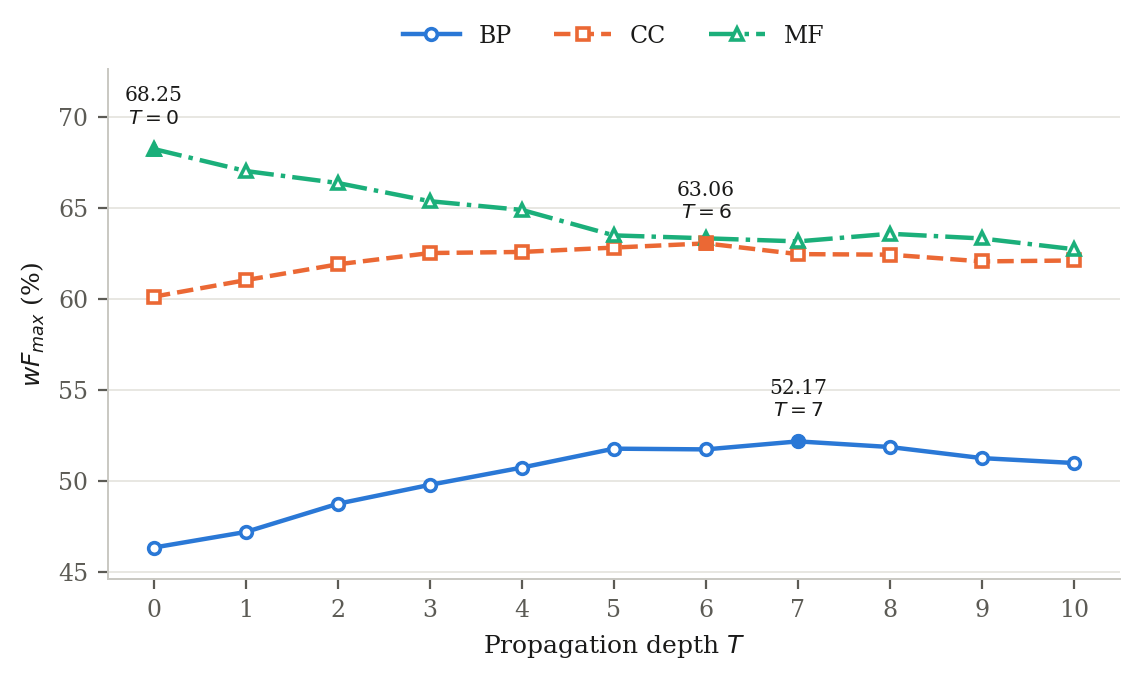
\includegraphics[width=0.92\textwidth]{fig_hops_visual}
  \caption{Propagation depth versus $wF_{\max}$ with the vision head (validation set,
  $\alpha = 0.5$). The peak lies at $T=7$ for BP, $T=6$ for CC and $T=0$ for MF.}
  \label{fig:hops_vision}
\end{figure}


\begin{figure}[!htb]
  \centering
  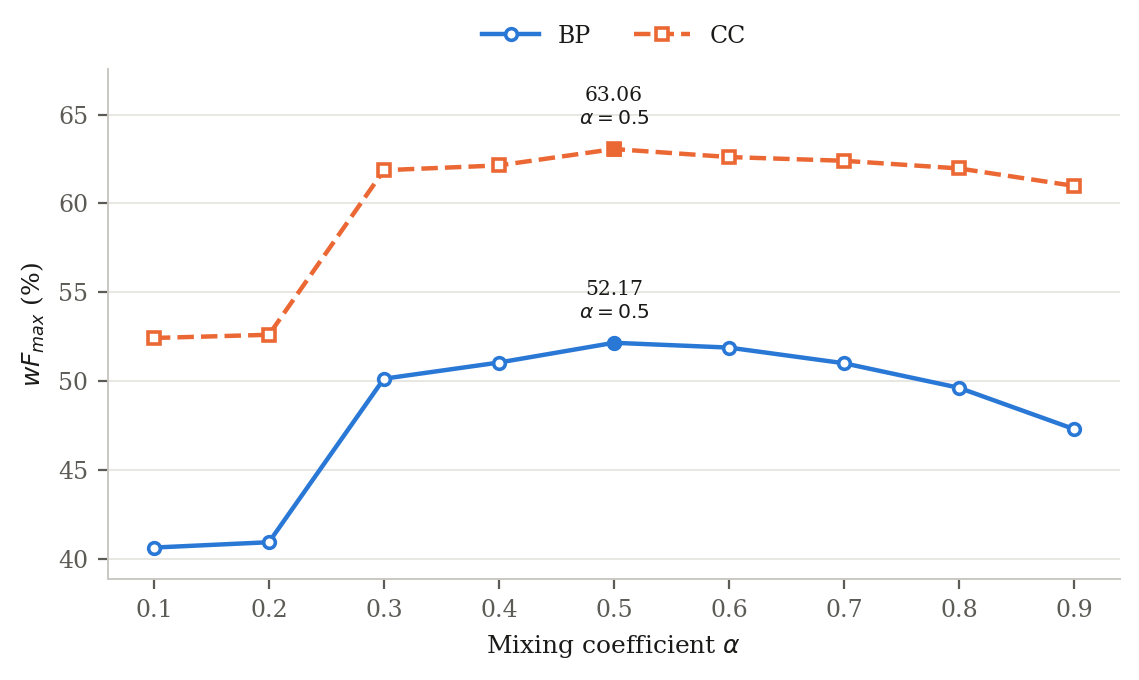
\includegraphics[width=0.92\textwidth]{fig_alpha_visual}
  \caption{Mixing coefficient versus $wF_{\max}$ with the vision head (validation set),
  at the best depth of each ontology. The collapse below $\alpha = 0.3$ is the
  annihilation of the node's own contribution, which decays as $\alpha^{T}$.}
  \label{fig:alpha_vision}
\end{figure}

The vision route inverts the depth conclusion. Where the vector head peaks at one or two
steps, the vision head peaks at $T=7$ in BP and $T=6$ in CC, and gains far more from
propagation: $5.84$~pp in BP and $2.93$~pp in CC over the graph-free control, against
$1.85$ and $0.92$ for the vector head. It also decays far less, $1.19$~pp in BP and
$0.94$~pp in CC between the peak and $T=10$, against $13.60$ and $12.80$~pp for the vector
head. The curve is not so much a peak as a plateau: in BP every depth from $T=5$ to $T=9$
lies within $0.92$~pp of the optimum, and in CC every depth from $T=3$ onwards lies within
$0.99$~pp.

The reading is not that the vision head uses the graph better. It is that it uses the node
attribute worse. A route that extracts less from the protein's own embedding has less to
lose when diffusion dilutes it, and more to gain from the neighborhood average. The
absolute values make the point: the vision peak in BP, $52.17$, sits below the vector
route's graph-free control at $53.36$. Deep propagation buys the vision head a recovery it
would not need with a better head.

MF again peaks at $T=0$ in both routes, and that two heads with very different
sensitivities to propagation agree on it is the strongest form the observation takes.

The mixing coefficient tells the complementary half of that story, and it does so by
inverting what a partial sweep had suggested. Over the full range the vision route is more sensitive to $\alpha$ than the vector one, not less: an amplitude of
$11.51$~pp in BP and $10.62$~pp in CC, against $5.51$ and $8.45$ for the vector head. The
mechanism is the depth at which each route operates. For a node whose aggregation is empty
(and between $32$ and $38$ percent of the nodes in each ontology are in that position)
the operator reduces to $\mathbf{H} \leftarrow \alpha^{T}\mathbf{H}$, so the node's own
contribution decays as a power of the depth. At $T=7$ a setting of $\alpha = 0.1$
scales that contribution by $10^{-7}$; at $T=1$ it retains a tenth of it. The collapse at
$\alpha \leq 0.2$ in Table~\ref{tab:sweep_alpha_vision} ($40.66$ in BP against $52.17$
at the optimum, a loss of $11.51$~pp) is that annihilation made visible.

Sensitivity to $\alpha$ is therefore not a property of the head but a consequence of the
depth the head prefers. The two routes converge on the same underlying constraint from
opposite directions: the vector head protects the node representation by propagating
shallowly, and the vision head, propagating deeply, must protect it through $\alpha$
instead. Both peak where retention is high ($\alpha = 0.7$--$0.8$ for the vector route
at $T \leq 2$, $\alpha = 0.5$ for the vision route at $T \geq 6$) and both degrade
sharply once the node's own signal is allowed to vanish.

One caveat on reading the AVG column of Table~\ref{tab:sweep_hops_vision}: its maximum
falls at $T=4$, a depth that is optimal for no individual ontology. The column averages
three curves whose peaks lie at $T=7$, $T=6$ and $T=0$, and its maximum is an artifact of
that mixture rather than a recommended setting.

\subsection{End-to-End Graph Learning}
\label{sec:gnn}

Table~\ref{tab:gnn_gcn_gat} replaces the fixed operator with a graph encoder trained
jointly with the classifier.

\begin{table}[!htb]
  \centering
  \caption{End-to-end graph representation learning ($wF_{\max}$, validation set). Both encoders consume the same graph and the same ProtT5 node attributes, and their trainable transformations are optimized end to end. GAT additionally learns attention coefficients, whereas GCN uses fixed degree-normalized edge weights. Best per column in bold, second best underlined.}
  \label{tab:gnn_gcn_gat}
  \begin{tabular}{llcccc}
    \toprule
    Graph Encoder & Prediction Head & BP & CC & MF & AVG \\
    \midrule
    \multirow{2}{*}{GCN (2 layers)} & Vector & \textBF{55.78} & \textBF{66.35} & \textBF{67.83} & \textBF{63.32} \\
     & Vision & \underline{53.10} & \underline{63.33} & \underline{65.46} & \underline{60.63} \\
    \midrule
    \multirow{2}{*}{GAT (2 layers, 4 heads)} & Vector & 46.47 & 61.14 & 63.83 & 57.15 \\
     & Vision & 46.17 & 59.45 & 61.03 & 55.55 \\
    \bottomrule
  \end{tabular}
\end{table}

This table offers six paired comparisons in which GCN and GAT differ in nothing but the
encoder, two prediction heads across three ontologies, and GCN wins all six, by
$3.88$ to $9.31$~pp. Section~\ref{sec:early_fusion} reproduces the ordering on the thirty
pairs its own grid affords, without a single inversion in either place.
GAT exists to learn edge weights that improve on those
supplied by the graph, and here the supplied weights are STRING combined scores, which are
themselves aggregated evidence rather than raw counts. The result says that the attention
mechanism, given the training signal available, does not recover a weighting better than
the one it was handed; and it pays for the attempt, as Section~\ref{sec:custo} quantifies.
A plausible explanation, which these experiments suggest rather than establish, is sample size in the relevant sense: the loss is masked to training vertices, so the attention parameters receive gradient only through the receptive field of the labeled nodes, two hops wide with two layers, while the STRING score already summarizes evidence from experiments, databases and text mining across the whole graph.

The comparison against the fixed operator is closer than the architecture would suggest.
Taking the champion of each family in each ontology, the learned encoder scores $63.32$ on
the three-ontology mean against $65.12$ for fixed propagation. It is ahead in BP by
$0.55$~pp, a margin at the interpretability floor and too small to read under the single-seed
design, and behind in CC by $0.59$~pp and in MF by $5.35$~pp. Learned aggregation therefore matches the fixed operator in one ontology
and loses in the other two, and the loss in Molecular Function is an order of magnitude
larger than the only margin it wins by. Section~\ref{sec:custo} adds the cost of each.

\subsection{Edge Deduplication}
\label{sec:dedup}

Summing repeated edges was the initial methodological choice of this work, and it is the
rule under which the results published at VISAPP~\cite{mauhnoom2026graphs} were produced. It
was changed for the campaign reported in this chapter, and the reason is a property of the
interaction file rather than a result.

\begin{table}[!htb]
  \centering
    \caption{Record multiplicity in the inherited STRING interaction file. Every repetition of a
  pair carries the same combined score, so multiplicity adds no score information.}
  \label{tab:rede_ppi}
  \begin{tabular}{lr}
    \toprule
    & Measured \\
    \midrule
    Rows in \texttt{ppi.csv} & $2{,}422{,}234$ \\
    Distinct pairs & $791{,}011$ \\
    Mean multiplicity (maximum) & $3.062$ ($170$) \\
    Pairs with divergent score across repetitions & \textBF{$0$} \\
    Score range & $[0.400,\ 0.999]$ \\
    \bottomrule
  \end{tabular}
\end{table}

Table~\ref{tab:rede_ppi} counts it. The file holds $2{,}422{,}234$ rows for $791{,}011$
distinct pairs, a mean multiplicity of $3.06$ and a maximum of $170$, and not one
pair disagrees with itself on the combined score. Multiplicity provides no additional score information, and its provenance cannot be established from the inherited file. Treating it as independent evidence is therefore unjustified. Summing gives a pair
the weight $c_{ij}\,s_{ij}$, and because $c_{ij}$ varies among the neighbors of the same
vertex, the column-stochastic normalization applied afterwards does not cancel it: the
ordering of a vertex's neighbors changes according to how many times each edge happened to
be written down. Taking the maximum is the rule that does not treat multiplicity as evidence.

That argument is analytic and it is the reason the rule was changed.
Table~\ref{tab:dedup} asks the separate question of whether the change moved any number.

\begin{table}[!htb]
  \centering
  \caption{Edge deduplication regime ($wF_{\max}$, validation set). Each cell is the champion of its family under that regime, selected by validation $wF_{\max}$. $\Delta$ is $\max$ minus $\mathrm{sum}$ on the AVG column, in percentage points.}
  \label{tab:dedup}
  \small
  \resizebox{\textwidth}{!}{%
  \begin{tabular}{lcccc|cccc|c}
    \toprule
    \multirow{2}{*}{Route} & \multicolumn{4}{c|}{$\max$} & \multicolumn{4}{c|}{$\mathrm{sum}$} & \multirow{2}{*}{$\Delta$} \\
    \cmidrule(lr){2-5} \cmidrule(lr){6-9}
    & BP & CC & MF & AVG & BP & CC & MF & AVG & \\
    \midrule
    Fixed propagation + vector head & 55.23 & 66.94 & 73.18 & 65.12 & 55.49 & 67.17 & 73.45 & 65.37 & -0.25 \\
    Fixed propagation + vision head & 52.17 & 63.06 & 68.25 & 61.16 & 52.60 & 62.82 & 68.89 & 61.44 & -0.28 \\
    End-to-end GCN + vector head & 55.78 & 66.35 & 67.83 & 63.32 & 55.31 & 65.77 & 68.26 & 63.11 & +0.21 \\
    End-to-end GCN + vision head & 53.10 & 63.33 & 65.46 & 60.63 & 51.39 & 62.60 & 64.91 & 59.63 & +1.00 \\
    End-to-end GAT + vector head & 46.47 & 61.14 & 63.83 & 57.15 & 49.17 & 59.17 & 61.05 & 56.46 & +0.69 \\
    End-to-end GAT + vision head & 46.17 & 59.45 & 61.03 & 55.55 & 45.56 & 56.00 & 53.60 & 51.72 & +3.83 \\
    \bottomrule
  \end{tabular}}
  \par\smallskip\footnotesize\raggedright Early and late fusion are absent because no hybrid or ensemble run exists in the $\mathrm{dedup}=\mathrm{sum}$ block.
\end{table}

The two columns do not report the same configurations. On the $\max$ side the
fixed-propagation rows carry the champions selected in
Section~\ref{sec:fixa}: with the vector head, $T=1$ and $\alpha=0.7$ in
BP, $T=2$ and $\alpha=0.8$ in CC, and $T=0$ in MF; with the vision head, $T=7$ and
$\alpha=0.5$ in BP, $T=6$ and $\alpha=0.5$ in CC, and $T=0$ in MF. On the
$\mathrm{sum}$ side they are the configurations the earlier generation settled on: vector
head at $T=1,\ \alpha=0.5$ in BP, $T=1,\ \alpha=0.6$ in CC and $T=0$ in MF; vision head at
$T=5,\ \alpha=0.5$ in BP, $T=6,\ \alpha=0.4$ in CC and $T=0$ in MF. The four GNN rows carry
neither depth nor mixing coefficient, since their aggregation is learned rather than fixed.

For the fixed-propagation rows, this accounting does introduce a hyperparameter confound: the $\max$ and $\mathrm{sum}$ campaigns use different selected values of depth and mixing coefficient. Those rows therefore compare the champions obtained under each deduplication regime rather than isolating deduplication as a single experimental factor. The GNN rows provide a cleaner comparison in this respect, because depth and mixing coefficient do not apply to them; both regimes otherwise use the same $256$ batch size and $250$ epoch budget.

Two cells make the residual noise measurable. In MF both
heads are compared at $T=0$, and at $T=0$ the propagation operator is the identity: the
graph does not enter the computation, and the deduplication rule cannot change the result
by any amount. Whatever those two cells show is therefore not the rule. With the vector head
they differ by $0.27$~pp and with the vision head by $0.64$~pp, in both cases in favor of
$\mathrm{sum}$. That is the observed campaign-level discrepancy of a comparison between two campaigns run
months apart, and it is of the same order as the interpretability floor used throughout the
chapter.

Against that floor the column is legible. Three routes clear $0.64$~pp, and all three favor
$\max$: the end-to-end GCN with the vision head by $1.00$~pp, the GAT with the vector head by
$0.69$~pp, and the GAT with the vision head by $3.83$~pp, the last of these six times the
that $0.64$~pp tolerance. The other three routes (fixed propagation with either head, and the GCN
with the vector head) fall inside the floor at $-0.25$, $-0.28$ and $+0.21$~pp, and are
ties.

The split between the two groups is not arbitrary. The routes that are indifferent to the
rule are the two that apply a fixed operator, and the one learned encoder that aggregates
with unparameterized weights; the routes that gain are the learned ones, and among those the
GAT gains more than the GCN in both heads. That is what the normalization argument predicts.
Fixed diffusion applies the same normalization procedure under either deduplication rule, which may attenuate the effect of multiplicity after normalization; a learned encoder has to fit its parameters against
the distorted weighting, and attention, which parameterizes the weights themselves, has the
most to lose. Depth is not the driver: fixed propagation with the vision head propagates
six and seven steps and is still indifferent.

One caveat attaches to the mean. The per-ontology deltas change sign in two of the six
routes, and in one of them by a wide margin (the GAT with the vector head loses
$2.70$~pp in BP and gains $2.78$~pp in MF), so in those rows the AVG column is averaging
disagreement rather than summarizing agreement.

The deduplication rule is therefore justified analytically, by the argument about
normalization, and the empirical record is consistent with it: every difference that clears
that $0.64$~pp tolerance favors $\max$, the routes it favors are the ones the argument
singles out, and the residual noise runs in the opposite direction, so it cannot be what
produces the gap. The rule stands on the argument; the table corroborates it.

\subsection{Early Fusion}
\label{sec:early_fusion}

Early fusion combines two representations of the same protein before the prediction head.
The first is the output of the fixed operator of Section~\ref{sec:fixa}, which
propagates the ProtT5 embedding over the STRING topology for $T$ steps with a mixing
coefficient $\alpha$ and learns nothing in the process. The second is the node embedding
produced by a graph neural network trained end to end, either the GCN or the GAT of
Section~\ref{sec:gnn}. Neither branch replaces the other: the fixed branch carries the
protein's own embedding corrected by its neighborhood, the learned branch carries a
neighborhood aggregation whose weights were fitted to the task, and early fusion joins the
two vectors with \texttt{add} or \texttt{concat} before a single head sees them.
Five choices define a configuration: the fusion operator, the graph encoder that produced
the learned embedding, the prediction head, and the two that the first version of this
campaign left tied to the head, namely the provenance of the learned embedding and the
source of the propagation hyperparameters of the fixed branch.
The learned embedding is produced by a GNN that was itself trained with a head, and that
head need not be the one that later consumes the embedding. Likewise the fixed branch
needs a depth and a mixing coefficient, and the optimum of the vector route
(Section~\ref{sec:hops}) differs from the optimum of the vision route. Holding both to the
head makes them invisible; crossing them makes each measurable. The complete grid is
$60$ runs; Tables~\ref{tab:early_fusion} and~\ref{tab:early_grid} report it in two passes.

\begin{table}[!htb]
  \centering
  \small
  \caption{Early fusion, best configuration of each cell ($wF_{\max}$, validation set). Each entry is the best of the four provenance and source combinations of Table~\ref{tab:early_grid}. Unless marked, the winner is the embedding trained with a vector head combined with the hyperparameters of the vector route; $^{\mathrm{v}}$ marks a cell won by the embedding trained with a \emph{vision} head, and $^{\mathrm{s}}$ a cell won by the hyperparameters of the \emph{vision} route. Best per column in bold, second best underlined.}
  \label{tab:early_fusion}
  \begin{tabular}{lll cccc}
    \toprule
    Fusion & Encoder & Head & BP & CC & MF & AVG \\
    \midrule
    \texttt{add}    & GCN & Vector & \textBF{56.52}    & \underline{67.07}$^{\mathrm{v}}$          & \textBF{73.81} & \textBF{65.80} \\
    \texttt{concat} & GCN & Vector & \underline{56.05} & \textBF{67.20}$^{\mathrm{v}}$ & \underline{73.78}$^{\mathrm{v}}$ & \underline{65.68} \\
    \texttt{concat} & GAT & Vector & 52.99             & 65.74$^{\mathrm{v}}$ & 72.41$^{\mathrm{v}}$ & 63.71 \\
    \texttt{add}    & GAT & Vector & 51.52             & 64.90                         & 70.57 & 62.33 \\
    \texttt{add}    & GCN & Vision & 53.17$^{\mathrm{s}}$ & 64.77                      & 69.52 & 62.49 \\
    \texttt{add}    & GAT & Vision & 47.43$^{\mathrm{s}}$ & 60.65$^{\mathrm{s}}$       & 62.98 & 57.02 \\
    \midrule
    \texttt{concat} & GCN / GAT & Vision & \textit{n/a} & \textit{n/a} & \textit{n/a} & \textit{n/a} \\
    \bottomrule
  \end{tabular}
  \par\smallskip\footnotesize\raggedright \textit{n/a}: concatenation is not defined for the
  vision head, whose input has image shape. In MF the two routes share the same optimum
  ($T=0$, $\alpha=0.5$), so the source axis collapses there and only the provenance axis is
  crossed.
\end{table}

Addition with a GCN and the vector head is best on the mean at $65.80$, ahead of the fixed
operator alone by $0.68$~pp and of the learned encoder alone by $2.48$~pp. Concatenation
with the same encoder and head reaches $65.68$, a difference of $0.12$~pp: the two fusion
operators remain indistinguishable at this resolution, and the choice between them cannot
be made on this evidence. Per ontology the gain over the better of the two fused components
ranges from $0.26$~pp in CC to $0.74$~pp in BP, with $0.63$~pp in MF.
The encoder separates without exception. Across the $30$ paired comparisons the complete
grid affords (same ontology, same operator, same head, same provenance, same source), the
GCN leads the GAT by $1.37$ to $8.22$~pp, winning $30$ of $30$. This reproduces inside
the fusion stage the ordering of Section~\ref{sec:gnn}, on a grid five times larger than
the one available there.

\begin{table}[!htb]
  \centering
  \small
  \caption{Early fusion with the GCN encoder: the provenance and source axes crossed ($wF_{\max}$, validation set). \emph{Provenance} is the head with which the consumed GNN embedding was trained; \emph{source} is the route whose depth and mixing coefficient the fixed branch uses. Best per column and head in bold.}
  \label{tab:early_grid}
  \begin{tabular}{ll ll ccc}
    \toprule
    Head & Fusion & Provenance & Source & BP & CC & MF \\
    \midrule
    \multirow{8}{*}{Vector}
      & \texttt{add}    & vector & vector & \textBF{56.52} & 66.86 & \textBF{73.81} \\
      & \texttt{add}    & vector & vision & 55.73 & 65.79 & \textit{n/a} \\
      & \texttt{add}    & vision & vector & 53.98 & 67.07 & 73.42 \\
      & \texttt{add}    & vision & vision & 52.96 & 65.46 & \textit{n/a} \\
      & \texttt{concat} & vector & vector & 56.05 & 67.12 & 73.68 \\
      & \texttt{concat} & vector & vision & 55.52 & 65.27 & \textit{n/a} \\
      & \texttt{concat} & vision & vector & 55.32 & \textBF{67.20} & 73.78 \\
      & \texttt{concat} & vision & vision & 53.23 & 65.42 & \textit{n/a} \\
    \midrule
    \multirow{4}{*}{Vision}
      & \texttt{add} & vector & vector & 52.36 & \textBF{64.77} & \textBF{69.52} \\
      & \texttt{add} & vector & vision & \textBF{53.17} & 64.71 & \textit{n/a} \\
      & \texttt{add} & vision & vector & 49.72 & 62.66 & 67.66 \\
      & \texttt{add} & vision & vision & 50.21 & 62.64 & \textit{n/a} \\
    \bottomrule
  \end{tabular}
  \par\smallskip\footnotesize\raggedright In MF the two routes share the optimum, so the
  source axis collapses and the two rows of each provenance would be identical; they are
  reported once. The GAT grid reproduces the same ordering on both axes and is omitted:
  it loses all $30$ paired comparisons against the GCN.
\end{table}

The two new axes behave differently from one another, and the difference is the finding of
this subsection.
Provenance is not head-specific. On the vision head the embedding trained with a
vector head wins $10$ of $10$ paired comparisons, by $1.86$ to $3.69$~pp, median
$2.91$~pp. There is no exception in either encoder. On the vector head the effect is
smaller and admits exceptions (median $1.68$~pp, winning $14$ of $20$), and it shrinks
as the encoder improves: with the GAT the median is $2.29$~pp and the win rate $8/10$, with
the GCN only $0.36$~pp and $6/10$. The reading is that a GNN supervised by a vector head
produces the better embedding, and that the routes which most need a better representation
are the ones that gain most from receiving it.
The propagation hyperparameters are head-specific. The vector head prefers its own
depth and coefficient in $16$ of $16$ paired comparisons, median $1.79$~pp. The vision head
is indifferent: median $-0.27$~pp over $8$ pairs, winning $2$ of $8$, a spread too small to interpret confidently under the single-seed design. 

Section~\ref{sec:hops} supplies the mechanism: the vision
route operates at $T \geq 6$, where the curve is a plateau rather than a peak, so which of
two plateau points it inherits changes little.
Taken together the two axes say that the fixed branch must be tuned for the head that will
consume it, while the learned branch should simply be the best embedding available,
whatever produced it. The single champion configuration of CC illustrates both at once:
concatenation, GCN, vector head, the vision-provenance embedding, and the vector route's hyperparameters.
The prediction head remains the largest single effect, though the margin narrowed once the
vision route was allowed the better embedding: with the GCN the vector head leads by
$3.31$~pp on the mean, against $5.31$~pp with the GAT. Section~\ref{sec:vetor_visao} takes
this up.

\subsection{Late Fusion}
\label{sec:late_fusion}

Late fusion combines the probability matrices of two already-trained routes, without
retraining either of them. The first is the champion of the non-parametric family of
Section~\ref{sec:fixa} with the vector head, that is $T=1$ and $\alpha=0.7$ in BP,
$T=2$ and $\alpha=0.8$ in CC, and $T=0$ in MF. The second is the champion of the
end-to-end family of Section~\ref{sec:gnn} with the same head, the two-layer GCN in all
three ontologies. Each route was trained once and produces a matrix of per-term
probabilities over the same proteins; the rules below operate on those two matrices alone.
Table~\ref{tab:late_fusion} compares eleven of them, from a single scalar interpolation to
five stacking meta-classifiers.

\begin{table}[!htb]
  \centering
  \caption{Late fusion strategies ($wF_{\max}$, validation set). Each rule combines the probability matrices of the fixed-propagation and end-to-end routes, both already trained. Best per column in bold, second best underlined.}
  \label{tab:late_fusion}
  \begin{tabular}{lcccc}
    \toprule
    Combination Rule & BP & CC & MF & AVG \\
    \midrule
    Linear interpolation ($\gamma$) & \textBF{57.96} & \textBF{68.79} & \textBF{74.44} & \textBF{67.06} \\
    Maximum & 57.35 & 67.79 & 72.59 & 65.91 \\
    Minimum & 56.38 & 68.09 & 72.69 & 65.72 \\
    IC sigmoid & 57.03 & 67.57 & 73.88 & 66.16 \\
    Degree sigmoid & 57.02 & 67.76 & 72.42 & 65.73 \\
    Master equation & 57.42 & 68.10 & 73.93 & \underline{66.48} \\
    \midrule
    Stacking (decision tree) & 56.22 & 67.35 & 73.76 & 65.78 \\
    Stacking (logistic regression) & \underline{57.53} & \underline{68.50} & 72.47 & 66.17 \\
    Stacking (MLP) & 56.92 & 68.12 & 73.92 & 66.32 \\
    Stacking (random forest) & 56.65 & 68.21 & 74.14 & 66.33 \\
    Stacking (gradient boosting) & 56.67 & 67.72 & \underline{74.18} & 66.19 \\
    \bottomrule
  \end{tabular}
  \par\smallskip\footnotesize\raggedright The ensemble search persisted $wF_{\max}$ only, so the comparison across strategies exists on that metric alone; the remaining five metrics were recomposed afterwards for the winning rule and appear in Section~\ref{sec:confronto}.
\end{table}

Linear interpolation wins all three ontologies and leads the second-best rule by
$0.58$~pp on the mean. A single scalar, $\gamma = 0.50$ in BP and $0.55$ in CC and MF,
beats the information-content rule, the degree rule, the master equation that combines
both, and five stacking variants including gradient boosting and a random forest.

The stacking models explain why. Each meta-classifier receives four features for every
protein--term pair: the probability assigned by the fixed-propagation route, the probability
assigned by the end-to-end route, the information content of the term, and the log-degree of
the protein in the thresholded graph. Their fitted importances place almost all the weight
on the first two, the two predicted probabilities themselves: the decision tree assigns
$0.960$ and $0.030$, the random forest $0.629$ and $0.359$. The other two, the information
content and the log-degree, receive $7.8\times10^{-6}$ and $0.010$ in the tree, $0.003$ and
$0.010$ in the forest. In these fitted tree-based models, the two auxiliary features receive negligible importance compared with the two base-model probabilities. This suggests that, under the present training setup, information content and log-degree add little to the combination decision. Once that is known, the failure of the elaborate rules is not surprising: they
are conditioning the combination on variables that do not predict which route is right.

One limitation attaches to this table. The ensemble fits $\gamma$ on validation, one
parameter more than the isolated models have. The gain of the ensemble over the better of
its two components is $2.18$~pp in BP, $1.85$~pp in CC and $1.26$~pp in MF; that margin
does not overturn the result, but the extra parameter should be stated.

\subsection{What the Second Generation Settles}
Four decisions carry forward. Propagation is worth one or two steps with the vector head
and six or seven with the vision head, and none at all in Molecular Function. Retention
dominates diffusion, which puts the mixing coefficient in the upper half of its range for
every configuration that uses one. Learned aggregation does not pay for itself against the
fixed operator, and within it the GCN dominates the GAT in every one of the thirty paired
comparisons the fusion grid affords. Fusing the two representations helps, and it depends
on where the learned embedding came from rather than on how the two are combined; fusing
their predictions helps more. The best configuration of the generation is the linear
ensemble, and Section~\ref{sec:confronto} reports it against the literature.

% =====================================================================

\section{Vector versus Spatial Inductive Bias}
\label{sec:vetor_visao}

Both generations carried a vision route alongside the vector one, and in both the vision
route lost. This section consolidates the comparison, which is a question of design rather
than of tuning: do the images the vision route consumes, the outer absolute-difference matrix of
the first generation and the reshaped embedding of the second, have spatial locality that a
convolutional backbone can exploit?
Each cell reports the champion of that head within that stage and ontology, selected on
validation, which is the same rule used everywhere else in this chapter. The three
ontologies rarely agree on a configuration, so a row may combine three of them; they are
named in Table~\ref{tab:vetor_visao_avg}.


\begin{table}[!htb]
  \centering
  \caption{Vector versus vision prediction head across the four experimental stages, per ontology ($wF_{\max}$, validation set). Each cell is the champion of that head in that stage and ontology; the configurations are named in Table~\ref{tab:vetor_visao_avg}. The winning head is in bold.}
  \label{tab:vetor_visao_ontologia}
  \begin{tabular}{llcccc}
    \toprule
    Stage & Prediction Head & BP & CC & MF & AVG \\
    \midrule
    \multirow{2}{*}{First Generation} & Vector & \textBF{36.37} & \textBF{48.25} & \textBF{48.92} & \textBF{44.51} \\
     & Vision & 30.40 & 40.84 & 42.42 & 37.89 \\
    \midrule
    \multirow{2}{*}{Fixed propagation} & Vector & \textBF{55.23} & \textBF{66.94} & \textBF{73.18} & \textBF{65.12} \\
     & Vision & 52.17 & 63.06 & 68.25 & 61.16 \\
    \midrule
    \multirow{2}{*}{End-to-end GNN} & Vector & \textBF{55.78} & \textBF{66.35} & \textBF{67.83} & \textBF{63.32} \\
     & Vision & 53.10 & 63.33 & 65.46 & 60.63 \\
    \midrule
    \multirow{2}{*}{Early fusion} & Vector & \textBF{56.52} & \textBF{67.20} & \textBF{73.81} & \textBF{65.84} \\
     & Vision & 53.17 & 64.77 & 69.52 & 62.49 \\
    \bottomrule
  \end{tabular}
\end{table}


\begin{table}[!htb]
  \centering
  \caption{Winning configuration of each prediction head at each stage and ontology, selected by validation $wF_{\max}$. In the early-fusion row, \emph{emb.} names the head with which the consumed GNN embedding was trained and \emph{hyp.} the route whose depth and mixing coefficient the fixed branch uses. $\Delta$ is vector minus vision on the three-ontology mean, in percentage points.}
  \label{tab:vetor_visao_avg}
  \small
  \resizebox{\textwidth}{!}{%
  \begin{tabular}{lp{5.2cm}cp{5.2cm}cc}
    \toprule
    Stage & Vector Configuration & AVG & Vision Configuration & AVG & $\Delta$ \\
    \midrule
    First Generation & MLP, \texttt{raw} (all three) & 44.51 & BP ConvNeXt-Tiny \texttt{avg}; CC ConvNeXt-Tiny \texttt{max}; MF ResNet-50 \texttt{avg} & 37.89 & +6.62 \\
    \midrule
    Fixed propagation & BP $T=1$, $\alpha=0.7$; CC $T=2$, $\alpha=0.8$; MF $T=0$ & 65.12 & BP $T=7$, $\alpha=0.5$; CC $T=6$, $\alpha=0.5$; MF $T=0$ & 61.16 & +3.96 \\
    \midrule
    End-to-end GNN & GCN (all three) & 63.32 & GCN (all three) & 60.63 & +2.69 \\
    \midrule
    Early fusion & BP \texttt{add}+GCN, vector emb., vector hyp.; CC \texttt{concat}+GCN, \emph{vision} emb., vector hyp.; MF \texttt{add}+GCN, vector emb. & 65.84 & BP \texttt{add}+GCN, vector emb., \emph{vision} hyp.; CC and MF \texttt{add}+GCN, vector emb., vector hyp. & 62.49 & +3.35 \\
    \bottomrule
  \end{tabular}}
  \par\smallskip\footnotesize\raggedright Because the selection is per ontology, the mean of
  a stage may exceed the mean of any single configuration held fixed across the three: the
  $65.84$ of early fusion combines two fusion operators, whereas the best configuration held
  fixed across the ontologies reaches $65.80$ in Table~\ref{tab:early_fusion}.
\end{table}

The vector head wins all twelve ontology-by-stage comparisons, with no exception in any
ontology at any stage. The margin narrows between the generations but does not close within
the second: it falls from $6.62$~pp in the topology-only generation to $3.96$~pp under fixed
propagation and $2.69$~pp for the learned encoder, then widens again to $3.35$~pp under early
fusion. Across the three stages of the second generation it sits in a band of $2.69$ to
$3.96$~pp with no trend toward zero, and early fusion, the strongest stage of the chapter,
still leaves $3.35$~pp on the table. Whatever the vision head is failing to capture, the
additional machinery of the second generation does not compensate for it.
The last row understates the deficit rather than exaggerating it. The vision champion of the
early-fusion stage consumes, in all three ontologies, an embedding trained with a
vector head; Section~\ref{sec:early_fusion} isolates that axis and measures the cost of
giving the vision route its own embedding instead at $1.86$ to $3.69$~pp. The comparison in
Table~\ref{tab:vetor_visao_ontologia} is therefore already generous to the vision head, which
is credited with the better representation the other head produced.
One row deserves a note. In the topology-only generation the vision champion is a different
backbone in each ontology, and in MF it is ResNet-50 rather than the ConvNeXt-Tiny adopted
for the second generation. That adoption was decided on the three-ontology mean, where
ConvNeXt-Tiny leads, and Section~\ref{sec:geracao1} states the margin it rests on.

The interpretation is that neither image the vision route consumes has the structure
convolution assumes. In the first generation the rows and columns are indexed by training
proteins in an arbitrary order; in the second, the pixels are embedding coordinates reshaped into
a $32 \times 32$ grid, adjacent only because of the order in which the ProtT5 dimensions happen to
be stored. In both cases adjacency in the image carries no meaning, and a convolutional kernel is
an operator that presumes it does. The MLP over the same information makes no such assumption. The
first generation's pooling ordering (\texttt{raw} above \texttt{max} above \texttt{avg})
points the same way, and so does the failure of the one-dimensional convolution there.
Three independent pieces of evidence, across two generations, agree that the inductive bias
of convolution is a mismatch for this representation.

% =====================================================================

\section{Comparison Against Adapted Literature Baselines}
\label{sec:confronto}

Tables~\ref{tab:confronto_bp} to~\ref{tab:confronto_mf} place NEXUS-GO against the five
reimplemented literature methods and the naive baseline, on all six metrics and one ontology
per table. Every value is measured on the held-out test partition, and the vision-head
variants are omitted, since Section~\ref{sec:vetor_visao} settles that the vector head wins
every stage-by-ontology comparison. Every row of the lower block is the champion of its
family, selected on validation and reported here without any further tuning. Two of them are
controls and carry no route name: First Generation, the best topology-only configuration of
Section~\ref{sec:geracao1}, and ProtT5 baseline, the fixed operator at $T=0$, where the graph
does not participate. The other four are the routes of the framework, named in
Section~\ref{sec:met_overview}: NEXUS-GO/Fixed and NEXUS-GO/GNN, the champions of
Sections~\ref{sec:fixa} and~\ref{sec:gnn}; NEXUS-GO/Early, the best cell of the fusion grid
of Section~\ref{sec:early_fusion}; and NEXUS-GO/Late, the linear interpolation that wins the
eleven combination rules of Section~\ref{sec:late_fusion}. The tables therefore read as a
single comparison on data that no decision of this work has seen.

\begin{table}[!htb]
  \centering
  \caption{Comparison against the reimplemented literature baselines in Biological Process (BP), test set. Six metrics; $S_{\min}$ is in bits and lower is better, all others are percentages and higher is better.}
  \label{tab:confronto_bp}
  \footnotesize
  \setlength{\tabcolsep}{4pt}
  \renewcommand{\arraystretch}{0.9}
  \begin{tabular}{lcccccc}
    \toprule
    Method & $F_{\max}$ & $F^{*}_{\max}$ & $wF_{\max}$ & AuPRC & IAuPRC & $S_{\min}\downarrow$ \\
    \midrule
    Naive baseline & 44.26 & 42.23 & 40.22 & 40.42 & 37.28 & 22.28 \\
    DeepGraphGO & 55.29 & 52.21 & 48.92 & 54.04 & 57.89 & 20.11 \\
    SEGT-GO & 52.05 & 48.22 & 44.57 & 42.82 & 50.71 & 21.24 \\
    Mashup & 43.58 & 41.86 & 39.64 & 34.82 & 32.57 & 23.22 \\
    MELISSA & 41.94 & 40.08 & 37.72 & 32.72 & 31.17 & 23.42 \\
    deepNF & 35.59 & 31.14 & 26.95 & 34.15 & 33.66 & 25.73 \\
    \midrule
    First Generation & 46.25 & 39.86 & 37.30 & 45.57 & 47.37 & 23.68 \\
    ProtT5 baseline & 59.61 & 56.31 & 53.74 & 58.53 & 62.92 & 18.92 \\
    NEXUS-GO/Fixed & 61.27 & 58.13 & 55.61 & 60.39 & 65.09 & 18.30 \\
    NEXUS-GO/GNN & 62.05 & 59.17 & 56.95 & 60.97 & \underline{66.27} & 17.66 \\
    NEXUS-GO/Early  & \underline{62.87} & \underline{59.81} & \underline{57.51} & \underline{62.42} & 65.73 & \underline{17.35} \\
    NEXUS-GO/Late & \textBF{63.74} & \textBF{60.96} & \textBF{58.69} & \textBF{64.02} & \textBF{68.83} & \textBF{17.12} \\
    \bottomrule
  \end{tabular}
  \par\smallskip\scriptsize\raggedright Best per column in bold, second best underlined. The naive baseline is excluded from the ranking.
\end{table}

\begin{table}[!htb]
  \centering
  \caption{Comparison against the reimplemented literature baselines in Cellular Component (CC), test set. Six metrics; $S_{\min}$ is in bits and lower is better, all others are percentages and higher is better.}
  \label{tab:confronto_cc}
  \footnotesize
  \setlength{\tabcolsep}{4pt}
  \renewcommand{\arraystretch}{0.9}
  \begin{tabular}{lcccccc}
    \toprule
    Method & $F_{\max}$ & $F^{*}_{\max}$ & $wF_{\max}$ & AuPRC & IAuPRC & $S_{\min}\downarrow$ \\
    \midrule
    Naive baseline & 58.43 & 56.52 & 48.13 & 56.26 & 51.22 & 10.84 \\
    DeepGraphGO & 73.74 & 71.11 & 60.35 & 71.88 & 78.59 & 9.67 \\
    SEGT-GO & 71.18 & 68.07 & 55.52 & 63.24 & 74.74 & 10.42 \\
    Mashup & 59.37 & 57.44 & 48.28 & 51.27 & 50.30 & 11.06 \\
    MELISSA & 58.54 & 56.51 & 47.19 & 49.78 & 48.97 & 11.23 \\
    deepNF & 62.49 & 57.59 & 36.51 & 58.44 & 65.10 & 13.52 \\
    \midrule
    First Generation & 67.38 & 63.46 & 48.39 & 63.83 & 72.20 & 12.03 \\
    ProtT5 baseline & 76.79 & 74.29 & 64.78 & 73.30 & 82.06 & 9.47 \\
    NEXUS-GO/Fixed & 78.20 & 75.85 & 66.93 & 74.32 & 83.78 & 8.85 \\
    NEXUS-GO/GNN & \underline{78.42} & 76.01 & 66.70 & \underline{74.41} & \underline{84.07} & \underline{8.44} \\
    NEXUS-GO/Early & \underline{78.42} & \underline{76.02} & \underline{67.18} & 74.33 & 83.72 & 8.57 \\
    NEXUS-GO/Late & \textBF{79.72} & \textBF{77.52} & \textBF{69.02} & \textBF{76.73} & \textBF{86.26} & \textBF{8.22} \\
    \bottomrule
  \end{tabular}
  \par\smallskip\scriptsize\raggedright Best per column in bold, second best underlined. The naive baseline is excluded from the ranking.
\end{table}

\begin{table}[!htb]
  \centering
  \caption{Comparison against the reimplemented literature baselines in Molecular Function (MF), test set. Six metrics; $S_{\min}$ is in bits and lower is better, all others are percentages and higher is better.}
  \label{tab:confronto_mf}
  \footnotesize
  \setlength{\tabcolsep}{4pt}
  \renewcommand{\arraystretch}{0.9}
  \begin{tabular}{lcccccc}
    \toprule
    Method & $F_{\max}$ & $F^{*}_{\max}$ & $wF_{\max}$ & AuPRC & IAuPRC & $S_{\min}\downarrow$ \\
    \midrule
    Naive baseline & 52.54 & 48.26 & 43.38 & 49.41 & 45.93 & 8.46 \\
    DeepGraphGO & 76.98 & 73.14 & 68.96 & 74.03 & 80.41 & 5.67 \\
    SEGT-GO & 73.40 & 68.76 & 64.12 & 58.64 & 75.15 & 6.37 \\
    Mashup & 54.52 & 49.82 & 44.22 & 47.87 & 47.29 & 8.30 \\
    MELISSA & 53.57 & 48.65 & 42.86 & 46.43 & 46.31 & 8.47 \\
    deepNF & 58.43 & 48.70 & 39.00 & 54.55 & 53.49 & 9.36 \\
    \midrule
    First Generation & 61.04 & 53.38 & 48.62 & 49.34 & 62.42 & 9.20 \\
    ProtT5 baseline & 79.75 & 76.02 & 72.57 & 73.75 & \underline{82.25} & 5.31 \\
    NEXUS-GO/Fixed & 79.75 & 76.02 & 72.57 & 73.75 & \underline{82.25} & 5.31 \\
    NEXUS-GO/GNN & 76.09 & 71.74 & 67.77 & 67.50 & 80.64 & 6.04 \\
    NEXUS-GO/Early & \underline{80.22} & \underline{76.54} & \underline{72.94} & \textBF{81.88} & 82.05 & \underline{5.22} \\
    NEXUS-GO/Late & \textBF{80.89} & \textBF{77.41} & \textBF{73.89} & \underline{76.53} & \textBF{84.92} & \textBF{5.14} \\
    \bottomrule
  \end{tabular}
  \par\smallskip\scriptsize\raggedright Best per column in bold, second best underlined. The naive baseline is excluded from the ranking.
\end{table}

The linear ensemble takes the best value of every column of the three tables, with a single
exception: AuPRC in MF, where early fusion leads it by $5.35$~pp. Its margin over the
strongest baseline is $9.77$~pp of $wF_{\max}$ in BP, $8.67$~pp in CC and $4.93$~pp in MF.
$S_{\min}$ agrees: $17.12$ against $20.11$ bits in BP, $8.22$ against $9.67$ in CC, $5.14$
against $5.67$ in MF.

The internal controls are as informative as the confrontation. The topology-only model of
the first generation trails the sequence-only control by $16.44$~pp in BP, $16.39$~pp in CC
and $23.95$~pp in MF, and the sequence-only control alone already exceeds the strongest
literature baseline in $wF_{\max}$ in all three ontologies. Most of the distance between this work and the
comparison methods is attributable to the protein language model, not to the graph
machinery built on top of it. The graph contributes the remainder, and
Section~\ref{sec:grau} shows on which proteins it contributes it.

One row pair requires a note. In Table~\ref{tab:confronto_mf}, \emph{ProtT5 baseline} and
\emph{NEXUS-GO/Fixed} carry identical values in every column, because they
are the same run: the
champion of the fixed-propagation family in MF is $T=0$, at which the propagation operator
is the identity. The duplication is a consequence of the result reported in
Section~\ref{sec:hops}.

% =====================================================================

\section{Cost, Connectivity and Coverage}
\label{sec:analise}

The previous sections established which route predicts best. This one asks at what price, on
which proteins, and over how much of the corpus. Section~\ref{sec:custo} measures the
training cost of each model family in seconds per epoch, hours per run and peak video memory,
which is what separates the fixed (i.e., non-parametric) operator from the trained graph encoder.
Section~\ref{sec:grau} breaks the test partition down by the connectivity of each protein and
asks where the interaction network actually contributes, a question the aggregate metrics of
Section~\ref{sec:confronto} cannot answer. Section~\ref{sec:cobertura} closes with the
fraction of the partition each method is able to score at all, which qualifies every margin
reported so far.

\subsection{Computational Cost}
\label{sec:custo}

Table~\ref{tab:custo} reports the cost of each model family. The campaign that supports the
tables of this chapter comprises $170$ runs. Of these, $147$ executed on the RTX A5500 and
are the ones timed here; the remaining $23$ are fixed-propagation vision runs that executed
on a GTX 1080 Ti, where the same configuration is about eight times slower, and mixing the
two would make the per-epoch column a function of which machine happened to be free rather
than of the model family.

\begin{table}[!htb]
  \centering
  \caption{Computational cost by model family, measured on the RTX A5500 ($147$ runs). Median seconds per epoch is the speed of the family; median hours per run folds in how many epochs each family needed before early stopping. Epochs is the median number of epochs actually executed, which exceeds the selected epoch of Table~\ref{tab:ape_custo} because training continues through the twenty epochs of early-stopping patience that follow the best one. VRAM is the peak of the family. Lowest value in bold for the three cost columns.}
  \label{tab:custo}
  \small
  \resizebox{\textwidth}{!}{%
  \begin{tabular}{lrrrrrr}
    \toprule
    Family & Runs & s/epoch & h/run & Total h & VRAM (GiB) & Epochs \\
    \midrule
    Fixed propagation + vector head & 49 & \textBF{5.24} & 0.35 & 15.1 & \textBF{6.4} & 250 \\
    Fixed propagation + vision head & 26 & 18.45 & 0.17 & 4.5 & \textBF{6.4} & 35 \\
    End-to-end GNN + vector head & 6 & 102.14 & 6.09 & 38.7 & 20.7 & 213 \\
    End-to-end GNN + vision head & 6 & 108.41 & 4.35 & 31.3 & 21.1 & 138 \\
    Early fusion + vector head & 40 & 5.26 & 0.27 & 10.2 & \textBF{6.4} & 205 \\
    Early fusion + vision head & 20 & 18.63 & \textBF{0.16} & 3.2 & \textBF{6.4} & 30 \\
    \midrule
    \textBF{Total} & \textBF{147} & & & \textBF{103.0} & & \\
    \bottomrule
  \end{tabular}}
  \par\smallskip\footnotesize\raggedright Hardware is described in Appendix~\ref{ape:implementacao}.
\end{table}

\begin{figure}[!htb]
  \centering
  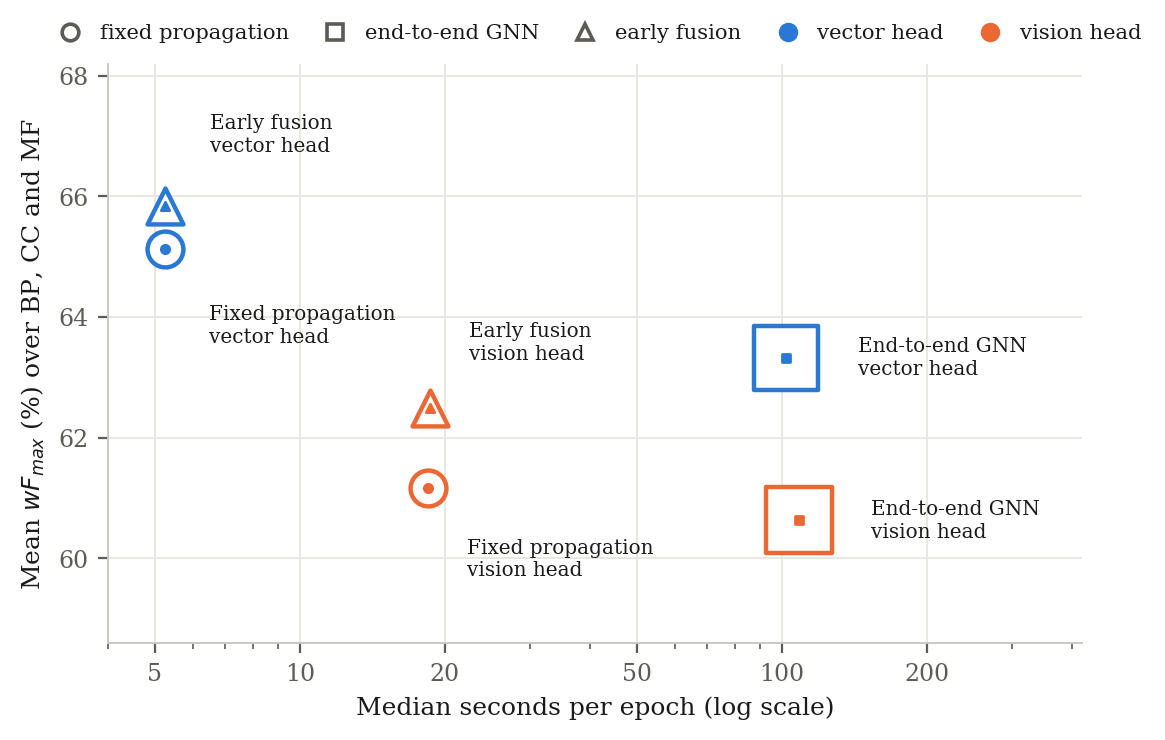
\includegraphics[width=0.92\textwidth]{fig_custo}
  \caption{Computational cost versus performance by model family. Median seconds per epoch
  on a logarithmic abscissa, mean validation $wF_{\max}$ over the three ontologies on the
  ordinate, marker area proportional to peak VRAM. Early fusion with the vector head
  occupies the upper-left region: as cheap as the cheapest family of the campaign and, on
  the three-ontology mean, the strongest of the non-ensemble routes.}
  \label{fig:custo}
\end{figure}

Figure~\ref{fig:custo} places the six families on the two axes that matter, cost against
performance, and the efficiency argument is best made per epoch, because the families differ
in how many epochs they need. Fixed propagation with the vector head trains at $5.24$ seconds
per epoch; the end-to-end encoder with the same head takes $102.14$, a factor of $19.5$. Peak
memory differs by a factor of $3.2$, $6.4$ against $20.7$~GiB. Both figures aggregate the two
learned encoders. Separating them, the graph convolution alone trains at $68.76$ seconds per
epoch and peaks at $14.1$~GiB over the three ontologies, and the attention operator at $161.41$
seconds and $20.7$~GiB, so most of the aggregate cost of the family is attributable to the
operator that Section~\ref{sec:gnn} shows does not pay for itself. The graph convolution is the
stronger of the two, and it matches the fixed operator in one ontology and loses in the other
two. A model that matches or beats that encoder while costing a thirteenth of the time per epoch
and less than half of its peak memory is the central practical claim of this work. The two hybrid families are included in the table; omitting them would understate the
argument, since early fusion attains the best non-ensemble mean at $5.26$ seconds per epoch
and $6.4$~GiB, which is the cost of fixed propagation itself: the two are within half a
percent of each other, and are jointly the cheapest of the six families. Adding the fixed
branch to a precomputed graph embedding is, in wall-clock terms, free. 

This comparison measures the marginal cost of training the fusion head once the GNN representation is already available. It does not include the upstream cost of training the GCN checkpoint from which the frozen embedding is extracted. Consequently, early fusion is nearly as cheap as fixed propagation only when that learned representation has already been computed.

\subsection{Connectivity and the Degree Paradox}
\label{sec:grau}

The remaining question is where the graph helps. Table~\ref{tab:rotas_conectividade}
identifies the five routes evaluated in this subsection: each is the champion of its family
in that ontology, selected on validation, and reported here on the test partition. Only the
vector head is carried into this analysis, since Section~\ref{sec:vetor_visao} settled the
comparison against the vision head in every stage and ontology.

\begin{table}[!htb]
  \centering
  \caption{The five routes evaluated in the connectivity analysis. Each is the champion of its family in that ontology, selected by validation $wF_{\max}$; the connectivity tables that follow report these runs on the test split. The trailing \texttt{\_embvision} marks the provenance of the consumed GNN embedding, as defined in Section~\ref{sec:early_fusion}.}
  \label{tab:rotas_conectividade}
  \scriptsize
  \resizebox{\textwidth}{!}{%
  \begin{tabular}{lccc}
    \toprule
    Route & BP & CC & MF \\
    \midrule
    ProtT5 only ($T=0$) & \texttt{fixed\_mlp\_h0\_a05} & \texttt{fixed\_mlp\_h0\_a05} & \texttt{fixed\_mlp\_h0\_a05} \\
    Fixed propagation + vector head & \texttt{fixed\_mlp\_h1\_a07} & \texttt{fixed\_mlp\_h2\_a08} & \texttt{fixed\_mlp\_h0\_a05} \\
    End-to-end GNN + vector head & \texttt{gnn\_gcn\_mlp} & \texttt{gnn\_gcn\_mlp} & \texttt{gnn\_gcn\_mlp} \\
    Early fusion + vector head & \texttt{hybrid\_add\_gcn\_mlp\_h1\_a07} & \texttt{hybrid\_concat\_gcn\_mlp\_h2\_a08\_embvision} & \texttt{hybrid\_add\_gcn\_mlp\_h0\_a05} \\
    First Generation & \texttt{MLP, raw} & \texttt{MLP, raw} & \texttt{MLP, raw} \\
    \bottomrule
  \end{tabular}}
  \par\smallskip\footnotesize\raggedright In MF the fixed-propagation champion is $T=0$, which makes it the same run as the graph-free control; the two rows coincide in that ontology, and the fixed route consumes no graph there.
\end{table}

\begin{table}[!htb]
  \centering
  \caption{Performance on isolated versus connected proteins ($wF_{\max}$, test set). A protein is isolated when its degree in the thresholded graph ($dedup = \max$) is zero: $3{,}421$ of $9{,}221$ in BP ($37.1\%$), $3{,}188$ of $9{,}292$ in CC ($34.3\%$) and $2{,}553$ of $7{,}864$ in MF ($32.5\%$). $\Delta$ is connected minus isolated, in percentage points. Best per column in bold, second best underlined.}
  \label{tab:degree_isolated_connected}
  \small
  \resizebox{\textwidth}{!}{%
  \begin{tabular}{lccccccccc}
    \toprule
    \multirow{2}{*}{Route} & \multicolumn{3}{c}{BP} & \multicolumn{3}{c}{CC} & \multicolumn{3}{c}{MF} \\
    \cmidrule(lr){2-4} \cmidrule(lr){5-7} \cmidrule(lr){8-10}
    & Isol. & Conn. & $\Delta$ & Isol. & Conn. & $\Delta$ & Isol. & Conn. & $\Delta$ \\
    \midrule
    ProtT5 only ($T=0$) & 59.89 & 50.23 & -9.66 & 69.30 & 62.38 & -6.92 & \textBF{75.68} & \underline{71.23} & -4.45 \\
    Fixed propagation + vector head & 61.30 & 52.39 & -8.91 & \textBF{71.12} & \underline{64.77} & -6.35 & \textBF{75.68} & \underline{71.23} & -4.45 \\
    End-to-end GNN + vector head & \underline{62.26} & \underline{53.97} & -8.29 & \underline{70.44} & 64.76 & -5.68 & \underline{74.99} & 64.30 & -10.69 \\
    Early fusion + vector head & \textBF{62.46} & \textBF{54.58} & -7.88 & 69.41 & \textBF{66.08} & -3.33 & 74.85 & \textBF{72.05} & -2.80 \\
    First Generation & 24.86 & 43.88 & +19.02 & 33.97 & 53.74 & +19.77 & 35.68 & 51.95 & +16.27 \\
    \bottomrule
  \end{tabular}}
\end{table}

Table~\ref{tab:degree_isolated_connected} contains a result that inverts the expected
picture. Every route that uses ProtT5 performs worse on connected proteins than on
isolated ones, in all three ontologies. The topology-only model does the opposite, by a
wide margin: it gains between $16.27$ and $19.77$~pp of $wF_{\max}$ moving from isolated to
connected proteins, which is exactly what a model whose only input is the graph should do:
with no neighbors its input vector is empty and only the prior remains.
The graph does narrow the gap. Early fusion has the smallest $\Delta$ of the sequence-aware
routes in all three ontologies ($-7.88$, $-3.33$ and $-2.80$ against the control's
$-9.66$, $-6.92$ and $-4.45$), so the deficit on connected proteins is roughly halved in CC and cut by about a third in MF. It is not eliminated in any of them.

Tables~\ref{tab:degree_f1_bp} to~\ref{tab:degree_f1_mf} resolve the effect by degree band.

\begin{table}[!htb]
  \centering
  \caption{Mean per-protein $F_1$ by connectivity degree band, BP ontology (test set; the routes are those of Table~\ref{tab:rotas_conectividade}). Best route per band in bold, second best underlined. Degree is measured on the full thresholded graph.}
  \label{tab:degree_f1_bp}
  \scriptsize
  \resizebox{\textwidth}{!}{%
  \begin{tabular}{lrccccc}
    \toprule
    Degree & $n$ & ProtT5 only ($T=0$) & Fixed + vec. & GNN + vec. & Hybrid + vec. & First Generation \\
    \midrule
    0 (isolated) & 3,421 & 59.64 & 61.45 & \underline{62.65} & \textBF{62.88} & 25.96 \\
    1--2 & 433 & 51.49 & 52.06 & \underline{52.71} & \textBF{53.17} & 34.31 \\
    3--5 & 757 & 47.56 & \textBF{49.33} & 47.86 & \underline{49.24} & 35.93 \\
    6--14 & 2,281 & 49.76 & 51.32 & \underline{52.08} & \textBF{53.55} & 41.37 \\
    15--49 & 2,066 & 51.70 & 54.31 & \underline{56.70} & \textBF{57.67} & 47.72 \\
    $\geq 50$ & 263 & 52.53 & 56.40 & \underline{60.31} & \textBF{61.58} & 52.63 \\
    \bottomrule
  \end{tabular}}
\end{table}

\begin{table}[!htb]
  \centering
  \caption{Mean per-protein $F_1$ by connectivity degree band, CC ontology (test set; the routes are those of Table~\ref{tab:rotas_conectividade}). Best route per band in bold, second best underlined. Degree is measured on the full thresholded graph.}
  \label{tab:degree_f1_cc}
  \scriptsize
  \resizebox{\textwidth}{!}{%
  \begin{tabular}{lrccccc}
    \toprule
    Degree & $n$ & ProtT5 only ($T=0$) & Fixed + vec. & GNN + vec. & Hybrid + vec. & First Generation \\
    \midrule
    0 (isolated) & 3,188 & 76.40 & \textBF{78.06} & \underline{77.95} & 76.98 & 57.99 \\
    1--2 & 380 & 68.61 & \textBF{70.79} & 69.32 & \underline{70.31} & 60.34 \\
    3--5 & 634 & 71.32 & \textBF{73.63} & 72.01 & \underline{73.30} & 64.24 \\
    6--14 & 2,357 & 69.96 & \underline{71.84} & 71.69 & \textBF{72.40} & 64.63 \\
    15--49 & 2,388 & 70.76 & 72.42 & \textBF{74.77} & \underline{74.24} & 67.37 \\
    $\geq 50$ & 345 & 66.55 & 68.42 & \textBF{75.26} & \underline{73.43} & 66.95 \\
    \bottomrule
  \end{tabular}}
\end{table}

\begin{table}[!htb]
  \centering
  \caption{Mean per-protein $F_1$ by connectivity degree band, MF ontology (test set; the routes are those of Table~\ref{tab:rotas_conectividade}). Best route per band in bold, second best underlined; \emph{ProtT5 only} and \emph{Fixed + vec.} are the same run in this ontology. Degree is measured on the full thresholded graph.}
  \label{tab:degree_f1_mf}
  \scriptsize
  \resizebox{\textwidth}{!}{%
  \begin{tabular}{lrccccc}
    \toprule
    Degree & $n$ & ProtT5 only ($T=0$) & Fixed + vec. & GNN + vec. & Hybrid + vec. & First Generation \\
    \midrule
    0 (isolated) & 2,553 & 78.05 & 78.05 & \underline{78.13} & \textBF{78.26} & 52.47 \\
    1--2 & 486 & \underline{75.89} & \underline{75.89} & 71.62 & \textBF{76.13} & 57.92 \\
    3--5 & 630 & \textBF{74.96} & \textBF{74.96} & 68.54 & \underline{74.63} & 55.79 \\
    6--14 & 1,952 & \underline{74.67} & \underline{74.67} & 69.82 & \textBF{75.73} & 57.77 \\
    15--49 & 1,945 & \underline{72.96} & \underline{72.96} & 67.45 & \textBF{74.69} & 56.47 \\
    $\geq 50$ & 298 & \underline{67.91} & \underline{67.91} & 65.93 & \textBF{72.55} & 54.19 \\
    \bottomrule
  \end{tabular}}
\end{table}

\begin{figure}[!htb]
  \centering
  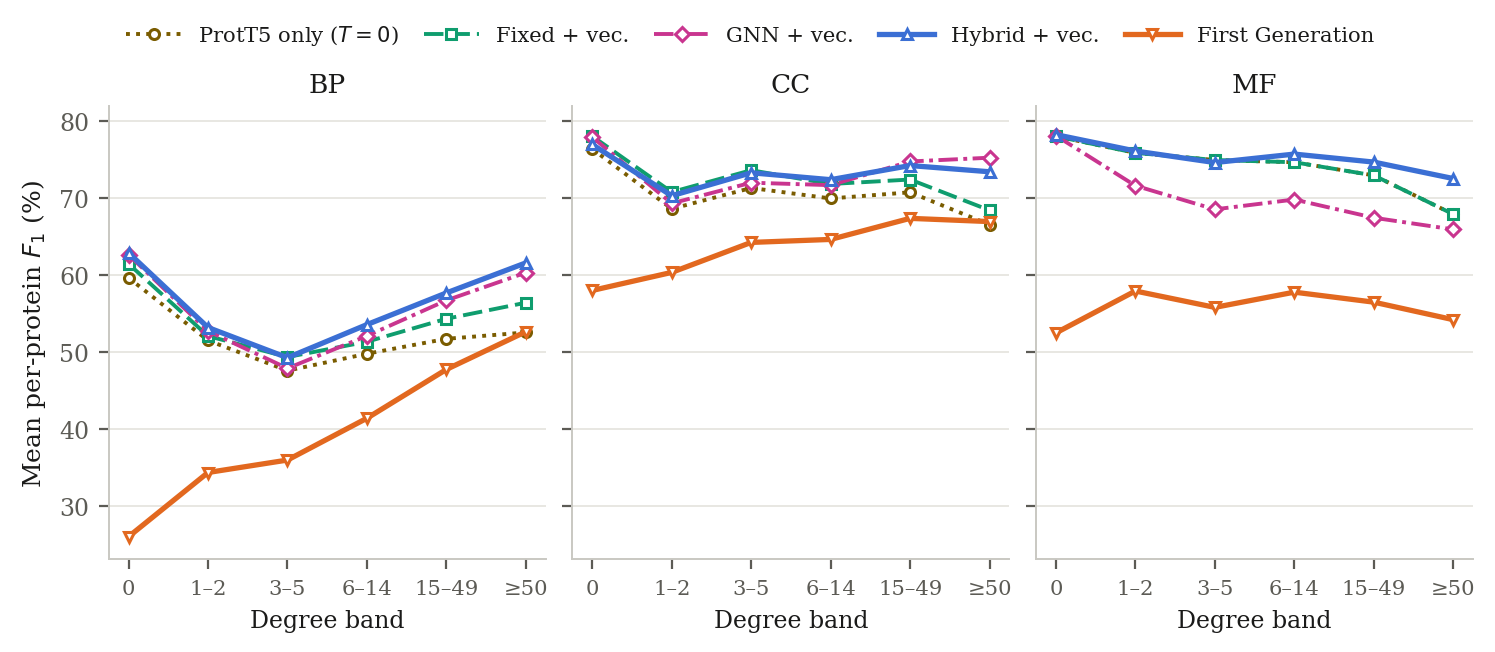
\includegraphics[width=\textwidth]{fig_grau}
  \caption{Mean per-protein $F_1$ by connectivity degree band (test set). In BP every
  sequence-aware route traces a U: the hardest proteins are not the isolated ones but those
  of degree three to five. The topology-only route traces no U in any ontology, and its
  worst band is the isolated one in all three. In MF \emph{ProtT5 only} and
  \emph{Fixed + vec.} are the same run, so their curves coincide.}
  \label{fig:grau}
\end{figure}

Figure~\ref{fig:grau} plots the three tables side by side, one panel per ontology. In BP the
curve is U-shaped for all four sequence-aware routes, and the minimum is not at
degree zero: it lies in the $3$--$5$ band, where every route scores between $12$ and
$15$~pp below its own isolated-protein figure. The worst-predicted proteins are the
sparsely connected ones, not the isolated ones. In CC the U appears only in the two routes
that carry a learned encoder, with the minimum in the $1$--$2$ band; the control and the
fixed route dip there as well but end lower still in the $\geq 50$ band, so their curves do
not close. MF shows no U at all: every sequence-aware route is at its best in the isolated
band and at its worst in the highest, with only a shallow rebound in the $6$--$14$ band for
the two routes that carry a learned encoder.

The shape is not created by the graph. The graph-free control traces the BP U by itself,
with no propagation of any kind, and the topology-only route, which is nothing but graph,
traces no U in any ontology: its worst band is the isolated one in all three, the exact
reverse of every sequence-aware route. Whatever
makes sparsely connected proteins hard is therefore a property of those proteins as seen by
a sequence model, and the graph inherits the problem rather than causing it.

\begin{table}[!htb]
  \centering
  \caption{Gain of the best graph-consuming route over the graph-free $T=0$ control, by connectivity degree band (mean per-protein $F_1$, test set, percentage points). The bracket names the route that attains it: \textsc{f} fixed propagation, \textsc{g} end-to-end GNN, \textsc{h} early fusion. In MF the fixed-propagation champion is $T=0$ and therefore identical to the control, so it is excluded from the maximum in that ontology.}
  \label{tab:degree_graph_gain}
  \small
  \begin{tabular}{lccc}
    \toprule
    Degree Band & BP & CC & MF \\
    \midrule
    0 (isolated) & +3.24\,\tiny{[\textsc{h}]} & +1.66\,\tiny{[\textsc{f}]} & +0.21\,\tiny{[\textsc{h}]} \\
    1--2 & +1.68\,\tiny{[\textsc{h}]} & +2.18\,\tiny{[\textsc{f}]} & +0.24\,\tiny{[\textsc{h}]} \\
    3--5 & +1.77\,\tiny{[\textsc{f}]} & +2.31\,\tiny{[\textsc{f}]} & $-$0.33\,\tiny{[\textsc{h}]} \\
    6--14 & +3.79\,\tiny{[\textsc{h}]} & +2.44\,\tiny{[\textsc{h}]} & +1.06\,\tiny{[\textsc{h}]} \\
    15--49 & +5.97\,\tiny{[\textsc{h}]} & +4.01\,\tiny{[\textsc{g}]} & +1.73\,\tiny{[\textsc{h}]} \\
    $\geq 50$ & +9.05\,\tiny{[\textsc{h}]} & +8.71\,\tiny{[\textsc{g}]} & +4.64\,\tiny{[\textsc{h}]} \\
    \bottomrule
  \end{tabular}
\end{table}

Table~\ref{tab:degree_graph_gain} makes the repair quantitative, and it is the cleanest
result of the subsection: the gain of the best graph-consuming route over the graph-free
control increases monotonically with degree from the $1$--$2$ band upward in BP and CC, and
from the $3$--$5$ band upward in MF. From the $1$--$2$ band to the highest it multiplies by
$5.4$ in BP, $4.0$ in CC and $19$ in MF. The graph helps where there is graph. That is
unsurprising as a direction and informative as a magnitude, and it explains the MF result of
Section~\ref{sec:hops} from a different angle: MF is the ontology where the gain is smallest
in every band, and the only one in which a band shows no gain at all.

Which route delivers the gain also moves with degree, and it moves in one direction. In CC
the fixed operator wins the three lowest bands and the learned encoder wins the two highest,
with early fusion in between; in BP early fusion wins five of six bands and the fixed
operator takes the $3$--$5$ band. The learned encoder pays off exactly where there is enough
neighborhood to learn from, which is the same boundary the depth analysis of
Section~\ref{sec:hops} found from the other side.

Two quantities in Table~\ref{tab:degree_correlation} need definition, because both are
internal to this analysis rather than campaign metrics. A model outputs a continuous score
for every protein--term pair, and precision and recall exist only once those scores are cut
into a set of predicted terms: $\tau$ is that cut. It is chosen per model as the value maximizing the mean per-protein $F_1$ on the partition reported. This mirrors the threshold-sweeping procedure used to define $F_{\max}$, although the statistic being optimized is different. The resulting $\tau$ should therefore be interpreted as a partition-specific diagnostic operating point rather than as a threshold selected for deployment. A single $\tau$ serves
all six degree bands of a given model, so differences between bands cannot be an artifact of
different cuts. The column is reported because $\tau$ varies widely between routes, from
$0.39$ to $0.63$, which is why no fixed cut would compare them fairly. And $\rho$ is
Spearman's rank correlation between a protein's degree and the $F_1$ the model achieves on
that protein: it works on ranks, so it asks whether better-connected proteins tend to be
predicted better without assuming the relation is linear. A negative $\rho$ says they tend
to be predicted worse.

\begin{table}[!htb]
  \centering
  \caption{Rank correlation between connectivity degree and per-protein $F_1$ (test set; the routes are those of Table~\ref{tab:rotas_conectividade}). $\rho$ is Spearman's rank correlation between degree and per-protein $F_1$; $\tau$ is the decision threshold that maximizes the mean per-protein $F_1$ of that model on this partition; $F_1$ is that mean, over all proteins of the partition. Best $F_1$ per ontology in bold, second best underlined.}
  \label{tab:degree_correlation}
  \small
  \resizebox{\textwidth}{!}{%
  \begin{tabular}{lccccccccc}
    \toprule
    \multirow{2}{*}{Route} & \multicolumn{3}{c}{BP} & \multicolumn{3}{c}{CC} & \multicolumn{3}{c}{MF} \\
    \cmidrule(lr){2-4} \cmidrule(lr){5-7} \cmidrule(lr){8-10}
    & $\tau$ & $\rho$ & $F_1$ & $\tau$ & $\rho$ & $F_1$ & $\tau$ & $\rho$ & $F_1$ \\
    \midrule
    ProtT5 only ($T=0$) & 0.51 & -0.109 & 53.84 & 0.58 & -0.129 & 72.29 & 0.50 & -0.128 & \underline{75.19} \\
    Fixed propagation + vector head & 0.50 & -0.105 & 55.77 & 0.63 & -0.133 & 74.07 & 0.50 & -0.128 & \underline{75.19} \\
    End-to-end GNN + vector head & 0.39 & -0.083 & \underline{56.96} & 0.51 & -0.087 & \textBF{74.68} & 0.51 & -0.185 & 71.79 \\
    Early fusion + vector head & 0.46 & -0.077 & \textBF{57.79} & 0.59 & -0.076 & \underline{74.46} & 0.42 & -0.110 & \textBF{76.11} \\
    First Generation & 0.41 & +0.415 & 36.62 & 0.46 & +0.161 & 62.94 & 0.49 & +0.083 & 55.44 \\
    \bottomrule
  \end{tabular}}
  \par\smallskip\footnotesize\raggedright This $F_1$ is the mean of a per-protein $F_1$ and is not comparable with the $F_{\max}$ of Section~\ref{sec:confronto}, which averages precision and recall separately before combining them. It is used here only to rank the routes within this analysis, where the same definition applies to all of them.
\end{table}

Table~\ref{tab:degree_correlation} rules out the explanation that first suggests itself. A
natural hypothesis is that aggregating over one or two neighbors dilutes a good
representation with noisy signal, and that this is what depresses the low-degree bands. If
that were the mechanism, the negative correlation would appear when propagation is switched
on. It does not: the graph-free control already has it, at $\rho = -0.109$ in BP, $-0.129$
in CC and $-0.128$ in MF. The best graph-aware route attenuates it in all three, to
$-0.077$, $-0.076$ and $-0.110$.

What the slope measures is therefore a property of the proteins rather than of the model.
Highly connected proteins tend to be multifunctional, carry more annotations, and are
intrinsically harder for a sequence-based predictor. The graph does not create that
difficulty; it partially repairs it.
Three further observations. First, the attenuation is a property of the best route, not of
propagation in general: in MF the learned encoder makes the slope markedly more
negative, $\rho = -0.185$ against $-0.128$ for the control, with mean $F_1$ falling from
$75.19$ to $71.79$, consistent with its $10.69$~pp loss on connected proteins in
Table~\ref{tab:degree_isolated_connected}; and in CC fixed propagation leaves the slope at
$-0.133$ against the control's $-0.129$, a difference too small to read as anything but
unchanged. Second, CC is the one ontology in which early fusion does not lead this table:
the learned encoder reaches $74.68$ against $74.46$, a gap of $0.22$~pp, and the two swap
places relative to the validation ranking of Section~\ref{sec:early_fusion}. 

The gains in the isolated band cannot be attributed to propagated neighborhood information. 
In the fixed route, the representation of a degree-zero protein changes by the $\alpha^{T}$ 
scaling described in Section~\ref{sec:met_fixa}, and each configuration trains a separate 
prediction head; in the hybrid route, the additional branch also changes model capacity. 
The degree-zero differences therefore combine rescaling, refitting, and, for the hybrid, 
additional capacity. A topological interpretation of the gains should begin with the 
degree-one-or-higher bands.
Three caveats apply to this reading. Degree is measured on the complete graph, over the
union of the three partitions, not against the training set alone. The $\geq 50$ band holds
between $263$ and $345$ proteins and is the least precise of the six, which is unfortunate
because it carries the largest gains. And the decision threshold is global per model rather
than per band, which is what makes the bands comparable but also means no band is evaluated
at its own optimum.

\subsection{Coverage}
\label{sec:cobertura}

A comparison of scores is only fair if the methods score the same proteins.
Table~\ref{tab:cobertura} reports what fraction of the test partition each family can
predict at all.

\begin{table}[!htb]
  \centering
  \caption{Prediction coverage of the test split by method family. A protein is covered when the method can produce a prediction for it; methods that consume only the interaction network cannot score a protein absent from their network. The test partition holds $9{,}221$ proteins in BP, $9{,}292$ in CC and $7{,}864$ in MF.}
  \label{tab:cobertura}
  \small
  \begin{tabular}{lrcrcrc} % <-- Alterado de lcccccc para lrcrcrc
    \toprule
    \multirow{2}{*}{Method Family} & \multicolumn{2}{c}{BP} & \multicolumn{2}{c}{CC} & \multicolumn{2}{c}{MF} \\
    \cmidrule(lr){2-3} \cmidrule(lr){4-5} \cmidrule(lr){6-7}
    & \% & $n$ & \% & $n$ & \% & $n$ \\
    \midrule
    DeepGraphGO / SEGT-GO & 96.3\% & 8,880 & 95.1\% & 8,837 & 95.7\% & 7,526 \\
    Mashup / MELISSA / deepNF & 63.6\% & 5,863 & 66.6\% & 6,187 & 68.7\% & 5,402 \\
    This work (all routes) & 100.0\% & 9,221 & 100.0\% & 9,292 & 100.0\% & 7,864 \\
    \bottomrule
  \end{tabular}
%\end{table}
  \par\smallskip\footnotesize\raggedright Mashup, MELISSA and deepNF consume only the interaction network and share the same limit; their counts are those of the evaluation itself. The DeepGraphGO and SEGT-GO counts are derived from the coverage fractions measured in this work and reported in Table~\ref{tab:ape_cobertura}, applied to the partition size; for the proteins outside their network these two transfer annotations by homology (PSI-BLAST) rather than discarding them.
\end{table}

Methods that build their representation only for proteins present in the interaction network cannot produce a prediction for a protein
absent from that network. Mashup, MELISSA and deepNF are all in this position and share the
same coverage limitation, between $63.6$ and $68.7$ percent of the test partition,
depending on the ontology. DeepGraphGO and SEGT-GO, which also read the sequence, reach
between $95.1$ and $96.3$ percent. Every route of this work covers the full partition,
because the ProtT5 embedding exists for every protein whether or not it has an edge.

This qualifies the confrontation of Section~\ref{sec:confronto}, and it does so against the comparative configurations rather than in their favor: as Appendix~\ref{ape:comparativos} records, every configuration was scored over the same complete test partition, so a protein a method cannot reach counts as a missed prediction rather than being removed from its score. The margins of Tables~\ref{tab:confronto_bp} to~\ref{tab:confronto_mf} therefore already carry the cost of that gap, and part of the distance to the three configurations of lowest coverage is coverage rather than ranking quality. The size of that effect is not hypothetical: the isolated proteins those three cannot reach are, in Table~\ref{tab:degree_isolated_connected}, the band on which every sequence-aware route scores highest.



% =====================================================================

\chapter{Conclusions}
\label{cap:conclusao}

In this research, we investigated how far a protein interaction network can go toward
predicting Gene Ontology annotations, first on its own and then combined with representations
learned by a protein language model. The work proceeded in two generations.

The first generation consumes no sequence information. It describes each protein by its
profile of STRING combined scores against the training set and asks how much of the
annotation that profile alone recovers. It reaches a mean $wF_{\max}$ of $44.51$ over the
three ontologies, $0.95$~pp above the term-frequency baseline that consumes no input at all,
a margin that is positive on the mean but negative in Biological Process, and it settles three design choices that the rest of the work inherits: the objective
function, the unreduced score profile with a vector head as the representation, and the
convolutional backbone of the image route. It also establishes the floor against which
everything built afterwards is measured, and it behaves on sparsely connected proteins in a
way no later model repeats.


The second generation places ProtT5 embeddings on the same STRING network, under the
transductive construction of Section~\ref{sec:met_transdutivo}, and it is where the
approach developed here is defined. We present NEXUS-GO (Network-Extended Unified Sequence
Embeddings for Gene Ontology function annotation), a framework that contextualizes those
embeddings with the weighted topology of the STRING network and that admits four routes: NEXUS-GO/Fixed, which propagates without learning the aggregation; NEXUS-GO/GNN, which applies
a graph encoder trained end to end; and NEXUS-GO/Early and NEXUS-GO/Late, which combine the two
at the representation and at the prediction level, respectively. Both generations were evaluated on
a multi-species corpus derived from CAFA5, under a single evaluation protocol, the second
generation transductively and the first under the stricter train-basis regime of
Section~\ref{sec:met_salvaguarda}, against a graph-free sequence control and five reimplemented
literature methods.


The contributions are the five announced in Chapter~\ref{cap:introducao}, and the
experiments of Chapter~\ref{cap:resultados} allow each of them to be stated with a result
attached.

The first is NEXUS-GO itself, whose core is the non-parametric multi-hop propagation
procedure that contextualizes ProtT5 embeddings with the weighted topology of the STRING
network. It trains no aggregation parameter and reaches a mean $wF_{\max}$ of $65.12$ against
$63.32$ for the graph convolution, the stronger of the two learned encoders, at a thirteenth
of the time per epoch and less than half of its peak memory.

The second is the controlled comparison between fixed propagation and learnable GCN- and
GAT-based aggregation under a common protocol, which shows that a graph encoder trained end
to end does not pay for itself here, and that the GCN encoder outperforms the GAT encoder in
all thirty-six paired comparisons of the campaign, by $1.37$ to $9.31$~pp.

The third is the evaluation of vector- and image-based classification heads over the same
contextualized embeddings. The direct vector head wins all twelve stage-by-ontology
comparisons on the primary metric, $wF_{\max}$, consistently outperforming the image-based
formulation across the four experimental stages.

The fourth is the development and evaluation of early- and late-fusion ensemble strategies
combining the fixed-propagation and GCN-based predictors. NEXUS-GO/Early gains $0.72$~pp on
the three-ontology mean over the better of the two representations it combines, with the
fusion operator selected per ontology, and the linear late-fusion ensemble, NEXUS-GO/Late,
gains between $1.26$ and $2.18$~pp over the better of its two components and is the strongest
configuration of the work.

The fifth is the benchmark against selected network-based state-of-the-art methods under the
same data splits and transductive setting, in which NEXUS-GO/Late leads the strongest
baseline by $9.77$, $8.67$ and $4.93$ percentage points of $wF_{\max}$ in BP, CC and MF, and
covers the whole test partition against $63.6$ to $96.3$ percent for the comparison methods.
The experiments further show that fixed propagation complements the sequence-derived features
in BP and CC, whereas its optimal depth is zero in MF. Graph information is therefore
substantially less useful for MF on the corpus evaluated here, although the fusion routes still
provide a modest improvement over the graph-free ProtT5 baseline.

At the end of this research, we can answer the questions formulated in
Chapter~\ref{cap:introducao}:

\begin{description}
\setlength{\itemsep}{4pt}\setlength{\parsep}{2pt}

\item[RQ1] \emph{How do different representations of the STRING PPI network data impact the
quality of functional prediction across the three GO domains?}

\textbf{Answer:} Under the evaluated configurations, the representation and its associated
inductive bias have a substantial effect on performance. The unreduced score profile leads the
pooled alternatives by up to $4.53$~pp on the three-ontology mean, and the evaluated
architectures that impose a one-dimensional ordering or a two-dimensional spatial locality on
coordinates that are training proteins in arbitrary order perform worse across the three
domains.

\item[RQ2] \emph{To what extent does fixed propagation of ProtT5 embeddings over the STRING
network improve upon the network-only representation, and how does this effect vary across
BP, MF, and CC?}

\textbf{Answer:} The improvement is large, but most of it is attributable to the sequence
embedding rather than to the propagation. The network-only route trails the graph-free
ProtT5 control by $16.44$~pp in BP, $16.39$~pp in CC and $23.95$~pp in MF on the test
partition; propagation then adds $1.87$~pp in BP and $2.15$~pp in CC over that control, and
nothing in MF, where the optimal depth is zero. The graph corrects the sequence
representation rather than replacing it.

\item[RQ3] \emph{How do different strategies, ranging from simple graph embeddings to fixed
non-parametric propagation and GNN approaches, compare under a common experimental protocol
and across vector- and image-based classification architectures?}

\textbf{Answer:} Ordered by mean validation $wF_{\max}$, the ensemble NEXUS-GO/Late leads at
$67.06$, followed by NEXUS-GO/Early at $65.84$, NEXUS-GO/Fixed at $65.12$ and NEXUS-GO/GNN at
$63.32$, while the graph-embedding methods of the literature fall below the term-frequency prior
in at least one domain. Among the routes evaluated with both classification heads, the ordering
holds for each of them.


\item[RQ4] \emph{Do early- and late-fusion ensembles improve the primary evaluation metric
over their individual fixed-propagation and GNN components?}

\textbf{Answer:} Both do, and combining predictions helps more than combining
representations. NEXUS-GO/Early gains $0.72$~pp on the three-ontology mean over the better of
the two representations it fuses, and the gain depends on the provenance of the learned
embedding rather than on the fusion operator. NEXUS-GO/Late gains $2.18$, $1.85$ and
$1.26$~pp over the better of its components, with a single scalar outperforming five stacking
meta-classifiers, at the cost of one parameter fitted on validation.

\item[RQ5] \emph{How do the propagation depth and the retention coefficient affect predictive
performance, and at what point does additional propagation begin to dilute the
protein-specific signal?}

\textbf{Answer:} With the vector head the optimum lies at one or two steps and dilution
begins immediately beyond it: performance falls by $13.60$~pp in BP, $12.80$~pp in CC and
$17.60$~pp in MF between the peak and ten steps. In BP and CC, retention dominates diffusion, with the
optimal coefficient lying between $0.7$ and $0.8$; in MF the optimal depth is zero and the
coefficient is therefore inapplicable. For a protein with no neighbors the operator
reduces to a multiplication by the coefficient raised to the depth, which is why deep
propagation with low retention annihilates it.

\item[RQ6] \emph{How does the proposed approach compare against established state-of-the-art
network-driven algorithms when all methods are evaluated using the same data splits and
transductive graph setting?}

\textbf{Answer:} NEXUS-GO/Late attains the best value of every column of the three
confrontation tables, one per domain, with a single exception: AuPRC in Molecular Function,
where NEXUS-GO/Early is ahead. Its
margin over the strongest baseline is $9.77$, $8.67$ and $4.93$~pp of $wF_{\max}$ on the test
partition, and the minimum semantic distance agrees.

\item[RQ7] \emph{Can the proposed methodology generalize effectively when applied directly to
global, aggregated-evidence networks, without the need to partition the graph by specific
species or evidence channels?}

\textbf{Answer:} The experiments show that NEXUS-GO operates effectively on a global,
multi-species network whose evidence channels have already been aggregated, and that it
requires no partitioning stage. In that setting it reaches the highest $wF_{\max}$ of the
comparison, while the configurations designed around multiple separate networks, deepNF among
them, are the ones that perform worst on it. What this establishes is the applicability of the
framework to the aggregated network used here, not that aggregation is superior or equivalent
to partitioning by species or by evidence channel: the counterfactual, running the framework
itself over partitioned graphs, was not executed and is one of the directions outlined below. %(AQUI EU JA ADCIONEI O DISCLAIMER E ELE INDICA UMA DIREÇÃO FUTURA DE LIMITAÇÕES DO TRABALHO)

\end{description}

Several limitations contextualize these conclusions. First, the experimental configurations were executed with a single seed. Consequently, the 0.5 percentage-point convention serves as a pragmatic reading threshold rather than a strict statistical confidence interval, and the adopted edge-deduplication rule rests primarily on normalization arguments rather than isolated empirical validation. Furthermore, the random protein-level partition does not enforce temporal, taxonomic, or sequence-similarity separation. This implies that the reported metrics primarily reflect transductive interpolation within the corpus, as validation and test nodes may share homologies or graph neighborhoods with the training set, and the reliance on the STRING combined score may introduce some degree of knowledge circularity.

Second, the comparison between fixed and learned routes should not be strictly viewed as a single-factor ablation, given inherent architectural differences regarding normalization, depth, and optimization---such as the scaling by $\alpha^T$ applied to isolated proteins by the fixed operator.  Regarding specific branches, graph information proved markedly less beneficial and more route-dependent in Molecular Function than in BP and CC: in MF no propagation depth improved upon the identity, and the learned encoder degraded the connectivity-accuracy relationship. Finally, because the baseline literature methods were reimplemented under the adapted conditions documented in Appendix~\ref{ape:comparativos} without common-coverage re-scoring, the reported performance ordering reflects these specific configurations and should not be directly transferred to the original published methods.

Several directions extend this work. The most immediate concerns the taxonomic scope: the corpus pools proteins from multiple species, although its taxonomic composition and the distribution of within- and cross-species edges were not characterized in this dissertation. Therefore, it remains open whether separating
the graph by organism, or keeping the graph whole and training one model per organism,
recovers signal that the aggregation dilutes. The two are not equivalent: the first changes
what a neighborhood is, the second what the classifier must generalize over.

A second direction concerns the evidence channels. The STRING combined score already
aggregates experimental interactions, curated databases, co-expression, genomic context and
text mining with heterogeneous reliability, and this work consumes it as a single weight.
Keeping the channels apart, as parallel graphs or as typed edges, would let the propagation
weigh experimental evidence differently from text mining and would make the contribution of
each source measurable.

That separation leads to a third direction, the heterogeneous graph. Proteins, functional
terms and evidence types can be modeled as distinct node and edge types in a single
structure, which this framework does not exploit; recent methods built on that formulation,
such as ProtHGT~\cite{ulusoy2025prothgt}, are the natural point of comparison and would also strengthen the
confrontation of Chapter~\ref{cap:resultados}.

A fourth direction concerns the graph encoder itself. The end-to-end variants evaluated here
aggregate over the complete neighborhood at every step, which makes them expensive and
exposes them to the dilution measured in Section~\ref{sec:hops}. Architectures based on
neighborhood sampling, GraphSAGE~\cite{hamilton2017graphsage} in particular, aggregate over a
bounded sample and may
combine the inductive advantage of a learned aggregation with a cost closer to that of the
fixed operator.

Finally, the characterization of the nodes can be broadened. Every second-generation route in
this work describes a protein through a single sequence-derived representation, formed by
concatenating the embeddings extracted from three ProtT5 layers, and the results indicate that
the quality of that representation strongly influences the performance of everything built on
top of it. Incorporating other biological sources, such as predicted three-dimensional
structure, domain composition or expression profiles, may provide complementary information
beyond sequence alone and could be particularly useful for Molecular Function, the domain in
which the interaction network contributes the least in the present experiments.


% As referências:
% Caso tenha usado o natbib, verifique o uso da linha abaixo para que as referências apareçam no sumário
% \addcontentsline{toc}{chapter}{\bibname}
\bibliographystyle{unsrt}
\bibliography{references}


% =====================================================================
% APPENDICES A AND B
% =====================================================================
% =====================================================================
\begin{appendices}{}
% =====================================================================

\chapter{Implementation Details and Reproducibility}
\label{ape:implementacao}

This appendix records the operational side of the experiments described in
Chapter~\ref{cap:metodologia}: the execution environment, the seeding mechanism, the optimization
settings, the cost of each family of model, and the artifacts each run produces. None of it changes
the definition of the methods; all of it is required to reproduce them.

\section{Computational Environment}
\label{ape:ambiente}

The experiments were executed across the local, server and hosted environments listed in
Table~\ref{tab:ape_maquinas}. The two server accelerators belong to the same physical node and are
reported separately because they executed different parts of the campaign. The table also identifies
the hosted Google Colab environment used for the first-generation image routes and for the
deepNF-derived configuration. The video memory reported there was read from the device at run time;
no manufacturer specification is quoted, since none was verified against the artifacts of this work.

\begin{table}[!htb]
  \centering
  \small
  \caption{Execution environments, with the video memory reported by the device and the part of the
  campaign each one executed. Device capacity is given in GiB.}
  \label{tab:ape_maquinas}
  \begin{tabular}{p{2.6cm}p{3.2cm}p{1.6cm}p{4.4cm}}
    \hline
    \textbf{Environment} & \textbf{Accelerator} & \textbf{Video memory} & \textbf{Role} \\
    \hline
    Server, shared node & NVIDIA RTX A5500 & $23.55$~GiB &
      Second generation: fixed propagation with both heads, graph convolutions, fusion \\[2pt]
    Server, same node & NVIDIA GTX 1080 Ti & $10.90$~GiB &
      Second generation: part of the fixed-propagation runs with the vision head \\[2pt]
    Local laptop & NVIDIA RTX 5060 Laptop & $7.96$~GiB &
      First generation: vector routes \\[2pt]
    Hosted, Google Colab & not recorded & not recorded &
      First generation: image routes; deepNF-derived configuration \\[2pt]
    Development machine & NVIDIA GTX 1050 Ti & $3.94$~GiB &
      Adapted comparative configurations \\
    \hline
  \end{tabular}
\end{table}

Two properties of this arrangement bear on the numbers reported in
Chapter~\ref{cap:resultados}. First, the server is a multi-GPU node shared with other users, so all
scripts fix \texttt{CUDA\_DEVICE\_ORDER=PCI\_BUS\_ID}: the default ordering does not follow the
numbering that \texttt{nvidia-smi} reports, and on a node whose cards belong to different
generations, selecting a device by index without fixing the ordering can dispatch a job to the wrong
card. Second, the two server cards belong to different architectures, and the GTX 1080 Ti has no
tensor cores, so mixed precision there reduces memory consumption without the throughput gain it
brings on the RTX A5500. Wall times measured on different environments are therefore not comparable
to one another, and Section~\ref{ape:custo} states which comparisons the measurements support.

Two memory conventions are used throughout and should not be conflated. The capacity of a device is
reported in GiB, as read from the device. The peak memory of a run is reported in MiB, which is the
unit under which each run recorded it; that quantity is the peak allocated by the training process
and is not the total occupancy of the card.

The available memory constrained the models in two distinct ways. On the development machine, the
node attribute matrix $\mathbf{H}^{(0)}$ of Equation~\eqref{eq:met_h0} occupies $1.13$~GB in single
precision for the $92{,}210$ proteins of Biological Process, and Equation~\eqref{eq:met_recorrencia}
requires a second buffer of the same size for the aggregation product. Those two tensors fit in
$3.94$~GiB, but they leave no headroom for the intermediate activations of a full-graph forward pass,
which scale with the number of vertices times the hidden width at every layer; Cellular Component
($1.14$~GB) and Molecular Function ($0.97$~GB) behave the same way. That machine was therefore
restricted to the adapted comparative configurations. On the server, the constraint persists at a
different scale: with $23.55$~GiB the graph attention operator reaches a peak of $18{,}864$~MiB for
Biological Process with gradient checkpointing enabled in the convolution layers, and exceeds the
card without it. That is what bounds the graph convolutions to two layers in
Table~\ref{tab:ape_hp}, and the bound is tighter for attention than for the graph convolutional
operator, whose peak is $12{,}953$~MiB under the same conditions.

\section{Software Stack}
\label{ape:bibliotecas}

The environments differ because the machines do. The campaign environment is a Conda environment
named \texttt{ppi-gpu}, with Python 3.10, PyTorch with CUDA support, and PyTorch Geometric built
against that pair. The environment of the development machine, which serves the adapted comparative
configurations that run locally, pairs Python 3.10 with PyTorch 2.4.0 and CUDA 12.4, PyTorch
Geometric, and Deep Graph Library from the matching \texttt{torch-2.4/cu124} distribution. The
remaining dependencies are common to both: \texttt{transformers} for the ProtT5 encoder, NCBI
BLAST\texttt{+} for the homology step of DeepGraphGO and SEGT-GO, and NumPy, SciPy, pandas,
scikit-learn and Matplotlib for data handling, metric computation and figures. The exact package
versions of each environment, together with the hardware specification of each machine, are
available in the repository\footnote{\url{https://github.com/ymauhn/nexus-go}}.

Three compatibility constraints were encountered directly during the experiments. The first is the
PyTorch, PyTorch Geometric and Deep Graph Library triple: the sparse tensor interface and the
message-passing operators of the latter two are tied to a specific major version of the former, and
mismatching them produces import-time failures rather than silent numerical differences. The second is the NumPy version: the metric routine currently depends on \texttt{numpy.trapz}, which was deprecated in NumPy 2.0. For forward compatibility, the implementation should use \texttt{numpy.trapezoid}, introduced in NumPy 2.0, or the corresponding SciPy function. The third is the
ProtT5 checkpoint, which is identified by repository name rather than by a revision, as
Section~\ref{ape:prott5} records. Other package versions may also affect installation, numerical
behavior or performance, and are therefore recorded in the environment documentation of the
repository rather than argued about here.

One environment-level trap is worth recording, because it fails at run time rather than at
installation. The accelerator of the local laptop requires binaries compiled for CUDA 12.8 or
later; distributions built against earlier CUDA versions install without error and fail only when
the first kernel is launched. A separate environment was created for that machine for this reason.

\section{Reproducibility}
\label{ape:repro}

\paragraph{Seeding.} A single global seed, $1337$, is applied at the start of every run to the
Python \texttt{random} module, to NumPy, to PyTorch on the host and to PyTorch on the device, and the
cuDNN backend is placed in deterministic mode. Seeding the interpreter is not by itself sufficient,
because the data loaders spawn four worker processes and each worker inherits an independent random
state; the loaders therefore receive an explicit worker initialization function and an explicit
generator, so that the order in which training indices are delivered is a deterministic function of
the seed. The number of workers is held fixed at four for the same reason: changing it changes the
sequence of batches even under an identical seed. The comparative configurations of
Appendix~\ref{ape:comparativos} that expose a seed use $42$, the value of their reference
configurations.

\paragraph{What the seed does and does not fix.} A rerun loads the same fixed partition files,
initializes the model from the same seed and presents the training indices in the same order, so the
experimental conditions are reproducible in that sense. These settings make data ordering and
parameter initialization repeatable, but they do not force every CUDA operation to use a
deterministic kernel: training uses automatic mixed precision with dynamic loss scaling, and some of
the reduction kernels involved are not bit-reproducible. Consequently, bitwise identity across runs
or hardware platforms is not claimed, and two runs under the same seed can diverge in the last
decimal places. Deterministic kernels were not enforced, since doing so would have made the
full-graph forward pass of the learned route prohibitively slow. One consequence of mixed precision
is worth recording because it was verified rather than assumed: inside the graph convolution and
graph attention layers the message tensors remain in single precision even under autocast, because
the softmax of the graph library promotes the exponential to single precision.

\paragraph{Single-seed estimates.} Because each configuration was evaluated with a single seed, no
empirical estimate of run-to-run variability is available. The values reported in
Chapter~\ref{cap:resultados} are point estimates, not means over replicates, and no confidence
interval is attached to them. This trades statistical strength for coverage: the permutation table is
large enough that replicating every cell was not feasible within the available compute budget, and
replicating only a subset would produce a table in which some entries carry an interval and others do
not. Small numerical differences are therefore not interpreted as evidence of robust superiority
unless they are supported by consistent behavior across ontologies and across metrics.

\paragraph{Gradient checkpointing.} Checkpointing is enabled in the convolution layers, without which
the graph attention operator does not fit the server card. The random number generator state is
preserved across the recomputation, so the technique trades computation for memory and is not
intended to constitute a difference in treatment between the two operators.

\paragraph{Caching of the first-generation descriptors.} The routine that builds the interaction
profile of Equation~\eqref{eq:met_perfil} is a pure function of the protein identifier, the
partition, the pooling strategy and the output length, with no random component, and it was
originally re-executed at every epoch. Precomputing it once was checked against the uncached path,
and the metrics obtained by the two agreed to the precision at which they are reported. The check is
indirect, since it compares the end of the pipeline rather than the descriptor arrays themselves,
and it is reported here as the evidence that was actually collected.

\section{Extraction of the Sequence Representation}
\label{ape:prott5}

The definition of the node attribute belongs to Section~\ref{sec:met_prott5}. What follows is the
operation. The extraction procedure, including the sequence preprocessing and the chunking rule, is
inherited without modification from the released implementation of
SUPERMAGOv2\footnote{\url{https://github.com/gabrielbianchin/SUPERMAGOv2/blob/main/src/scripts/extract.py}}.

The checkpoint is \texttt{Rostlab/prot\_t5\_xl\_half\_uniref50-enc}, the encoder-only release of
ProtT5-XL-U50, loaded from Hugging Face revision \texttt{94a6abc029ae13029317b140b7424e012bf8dfbf} 
in \texttt{bfloat16}, with the weights never updated. Sequences are chunked into non-overlapping segments of at
most $1{,}022$ residues. The chunks are encoded in batches whose size varies between $256$ and $64$
across the campaign, according to the availability of the shared accelerator and the time budget of
each extraction; on a device out-of-memory error the batch size is halved and the batch retried, so
the extraction completes without manual intervention on machines of different capacities. The batch
size affects throughput only, since the encoder is frozen and each chunk is encoded independently.


The pooling is performed in two stages, and the distinction matters for long proteins. Within a
chunk, the per-residue hidden states of each of the three layers are averaged over the valid
positions, with padding excluded by the attention mask. Across the chunks of the same protein, the
resulting chunk-level vectors are then averaged with equal weight. This is the operation written in
Equation~\eqref{eq:met_meanpool}. For a protein short enough to fit in a single chunk the two stages
collapse into a masked mean over its residues; for a protein split into several chunks, the second
stage weights each chunk equally rather than by its length, so the residues of a short trailing
chunk carry more weight per residue than the rest.

The results are cached on disk as one file per layer per protein, in NumPy's binary format, in single
precision, named by the protein accession and the layer index (\texttt{<accession>-24.npy},
\texttt{-23}, \texttt{-22}). One directory is written per ontology. This yields three files per
protein per ontology, or $791{,}277$ files in total. Their contents occupy approximately $3.3$~GB,
but each file is smaller than two file-system blocks and larger than one, so the space actually
allocated is close to $6.5$~GB; the second figure is the one to plan for. The choice of one small
file per layer rather than a single consolidated array allows the three channels to be selected
independently at load time without rewriting the cache; the cost is the large number of inodes and
a load step dominated by file-system overhead rather than by bandwidth.

The loader that assembles $\mathbf{H}^{(0)}$ tolerates a missing file, substituting a zero vector
rather than aborting the run. No file was missing for any protein of the corpus, so this branch was
never taken. It is recorded here because it is a hazard for future reproductions rather than a
feature: a preprocessing failure would be silently converted into a protein that looks uninformative
instead of raising an error, and a reproduction should prefer to abort and report the affected
identifiers.

\section{Optimization Settings}
\label{ape:hiperparametros}

Table~\ref{tab:ape_hp} lists the settings of the final second-generation campaign. No automated
hyperparameter search was performed: the values were fixed by inspection of preliminary runs and
then held constant, so that a difference between two configurations in
Chapter~\ref{cap:resultados} reflects the factor being varied rather than an unequal search effort.
All proposed architectures therefore received the same fixed tuning budget and were not subjected to
architecture-specific searches. This improves the comparability of the experimental effort, but it
does not guarantee that the chosen settings are equally close to the optimum of every architecture,
and none of the reported numbers should be read as the best attainable by its architecture.

\begin{table}[!htb]
  \centering
  \caption{Optimization settings of the final second-generation campaign. Values marked ``varies''
  are part of the search space declared in Section~\ref{sec:met_espaco}. The first generation and
  the adapted comparative configurations use the settings documented separately below and in
  Appendix~\ref{ape:comparativos}.}
  \label{tab:ape_hp}
  \begin{tabular}{lll}
    \hline
    \textbf{Setting} & \textbf{Value} & \textbf{Scope} \\
    \hline
    Optimizer                     & Adam                        & all families \\
    Learning rate                 & $1 \times 10^{-4}$          & all families \\
    Weight decay                  & none                        & all families \\
    Learning-rate schedule        & none                        & all families \\
    Batch size                    & $256$                       & all families \\
    Maximum epochs                & $250$                       & all families \\
    Early-stopping patience       & $20$ epochs                 & all families \\
    Monitored quantity            & validation loss             & all families \\
    Minimum improvement           & $0$                         & all families \\
    Objective                     & Equation~\eqref{eq:met_proteinloss} & all families \\
    Class weighting               & information content         & all families \\
    Dropout, prediction head      & $0.4$                       & all families \\
    Dropout, between convolutions & $0.3$                       & graph convolutions \\
    Hidden widths, head           & $[1024,\,512]$              & all families \\
    Convolution hidden width      & $1024$                      & graph convolutions \\
    Convolution layers            & $2$                         & graph convolutions \\
    Attention heads               & $4$ (hidden), $1$ (output)  & graph attention \\
    Random seed                   & $1337$                      & all families \\
    Data-loading workers          & $4$                         & all families \\
    Configured edge threshold                & $0.10$ (inert; source-data floor = $0.400$)                       & all families \\
    Propagation steps $T$         & varies                      & fixed propagation \\
    Mixing coefficient $\alpha$   & varies                      & fixed propagation \\
    Deduplication rule            & varies                      & all families \\
    \hline
  \end{tabular}
\end{table}

Three entries deserve a comment. The objective is the composite loss of
Equation~\eqref{eq:met_proteinloss} in every run of the campaign, the only exception being the
explicit ablation against binary cross-entropy reported in Chapter~\ref{cap:resultados}. The hidden
widths of the prediction head are held at $[1024,\,512]$
for every family of this campaign, including early fusion, so that a difference between two fusion
operators cannot be attributed to a difference in head capacity. Earlier exploratory runs used a
wider head for the fusion family, and their numbers are consequently not comparable cell by cell
with those of the final campaign. And the first generation is a separate regime: its vector head is
the multilayer perceptron of Section~\ref{sec:met_gen1_vetor}, here with two hidden layers of
width $512$ and $256$, dropout at rate $0.5$ and no normalization layer, trained with a batch size
of $32$ for at most $200$ epochs with a patience of $25$. No table of this work crosses the two
regimes.


Table~\ref{tab:ape_hp} summarizes the principal settings but does not replace the configuration
files. The effective configuration of every run, after all command-line overrides, is recorded in
the manifest that run writes, and the configuration files themselves are available in the
repository.

The five stacking meta-classifiers of Section~\ref{sec:met_late} are fitted offline and share none
of the settings of Table~\ref{tab:ape_hp}, which describes neural training only. Their
configurations, and the grid over which the explicit fusion coefficients were searched, are reported
in Section~\ref{ape:fusao}.

% =====================================================================
% =====================================================================
\section{Fusion Hyperparameters}
\label{ape:fusao}

The explicit coefficients of the late-fusion rules of Section~\ref{sec:met_late} are chosen by
exhaustive search on the validation partition. Table~\ref{tab:ape_fusao_grade} gives the grid, which
is identical for the three ontologies: no per-ontology override was applied, and each ontology
enumerates the same $71$ configurations, $213$ over the three. None of them retrains a network,
because late fusion reads the probability matrices the base models have already written; only the
five meta-classifiers are fitted, and on CPU.

\begin{table}[!htb]
  \centering
  \small
  \caption{Search grid of the late-fusion coefficients. The same grid is applied to the three
  ontologies. The last column counts the configurations each rule contributes to the search.}
  \label{tab:ape_fusao_grade}
  \begin{tabular}{lp{6.4cm}r}
    \hline
    \textbf{Rule} & \textbf{Grid} & \textbf{Config.} \\
    \hline
    Linear combination            & $\gamma$ from $0.00$ to $1.00$ in steps of $0.05$ & $21$ \\
    Pointwise maximum and minimum & no parameter & $2$ \\
    Term-specific weighting       & $\mathrm{IC}_{\text{thr}} \in \{0.4,\,1.1,\,2.1,\,3.4\}$ and $\kappa_{\mathrm{IC}} \in \{1,\,2,\,5\}$ & $12$ \\
    Protein-specific weighting    & $d_{\text{thr}} \in \{1,\,3,\,5,\,14,\,28\}$ and $\kappa_{\deg} \in \{0.25,\,0.50,\,0.75,\,1.00\}$ & $20$ \\
    Combined weighting            & $\lambda$ from $0.0$ to $1.0$ in steps of $0.1$ & $11$ \\
    Stacking                      & five meta-classifiers, no coefficient swept & $5$ \\
    \hline
    \textbf{Total}                &                                              & \textbf{$71$} \\
    \hline
  \end{tabular}
\end{table}

The value $\kappa_{\deg} = 0$ is deliberately excluded. It makes $\beta_i$ constant at $1/2$ and
collapses Equation~\eqref{eq:met_ens_degree} onto the linear rule at $\gamma = 0.5$, so it does not
represent a distinct strategy. The search is staged rather than joint: the combined rule sweeps
$\lambda$ alone, with $\mathrm{IC}_{\text{thr}}$, $\kappa_{\mathrm{IC}}$, $d_{\text{thr}}$ and
$\kappa_{\deg}$ held at the values that won the term-specific and the protein-specific rules in that
ontology. Table~\ref{tab:ape_fusao_sel} reports the selected values.

\begin{table}[!htb]
  \centering
  \small
  \caption{Late-fusion coefficients selected on the validation partition, per ontology. The
  coefficients of the term-specific and protein-specific rules are also the ones the combined rule
  inherits.}
  \label{tab:ape_fusao_sel}
  \begin{tabular}{llrrr}
    \hline
    \textbf{Rule} & \textbf{Coefficient} & \textbf{BP} & \textbf{CC} & \textbf{MF} \\
    \hline
    Linear combination         & $\gamma$                       & $0.50$ & $0.55$ & $0.55$ \\
    \hline
    \multirow{2}{*}{Term-specific weighting}
                               & $\mathrm{IC}_{\text{thr}}$     & $1.1$  & $0.4$  & $0.4$ \\
                               & $\kappa_{\mathrm{IC}}$         & $1.0$  & $1.0$  & $1.0$ \\
    \hline
    \multirow{2}{*}{Protein-specific weighting}
                               & $d_{\text{thr}}$               & $3$    & $14$   & $28$ \\
                               & $\kappa_{\deg}$                & $0.25$ & $0.25$ & $0.25$ \\
    \hline
    Combined weighting         & $\lambda$                      & $0.5$  & $0.4$  & $0.9$ \\
    \hline
  \end{tabular}
\end{table}

\paragraph{Meta-classifiers.} The five models of Equation~\eqref{eq:met_ens_stack} are not searched:
their settings are fixed a priori and are the same in the three ontologies, as
Table~\ref{tab:ape_fusao_meta} records. Every one of them is fitted under the same random seed,
$42$, which also governs the rejection sampling that limits the negatives to five times the number
of positives.

\begin{table}[!htb]
  \centering
  \small
  \caption{Configuration of the five stacking meta-classifiers. All are fitted with random seed
  $42$ on the four features of Equation~\eqref{eq:met_ens_stack}, in the order in which that
  equation lists them.}
  \label{tab:ape_fusao_meta}
  \begin{tabular}{lp{9.2cm}}
    \hline
    \textbf{Meta-classifier} & \textbf{Settings} \\
    \hline
    Decision tree         & maximum depth $7$; balanced class weights \\
    Logistic regression   & standardized features; $C = 1.0$; at most $200$ iterations; balanced class weights \\
    Multilayer perceptron & standardized features; one hidden layer of width $8$; $L_2$ penalty $10^{-2}$; at most $200$ iterations; early stopping on a tenth of the fitting set \\
    Random forest         & $100$ trees; maximum depth $7$; balanced class weights \\
    Gradient boosting     & histogram-based; maximum depth $7$; learning rate $0.1$; at most $100$ iterations; balanced class weights \\
    \hline
  \end{tabular}
\end{table}

The node degree that Equations~\eqref{eq:met_ens_beta} and~\eqref{eq:met_ens_stack} consume is an
unweighted count of incident edges, so it is invariant to the deduplication rule of
Equation~\eqref{eq:met_dedup}: summation and maximum produce the same set of index pairs and differ
only in the weight attached to each.

Two properties of the selection deserve to be stated. The first is that both conditional rules
converged on the flattest sigmoid the grid offers: $\kappa_{\mathrm{IC}} = 1$ is the smallest of
$\{1,\,2,\,5\}$ and $\kappa_{\deg} = 0.25$ the smallest of $\{0.25,\,0.50,\,0.75,\,1.00\}$, in the
three ontologies and in both rules. A flat sigmoid produces a nearly constant weight, which makes
the term-specific and the protein-specific rules behave such as the linear rule with an extra
parameter. This corroborates, from the side of the search space, what the fitted importances of
Section~\ref{sec:late_fusion} show from the side of the models: the two auxiliary quantities carry
little that the two base probabilities do not already carry.

The second is that three of the six selections lie on the boundary of the grid. The information
content grid was calibrated on Biological Process, whose values reach $5.54$, and it does not cover
the range of the other two ontologies, which reach $9.79$ in Cellular Component and $9.26$ in
Molecular Function; both selected $\mathrm{IC}_{\text{thr}} = 0.4$, the lower edge, at which the
weight exceeds one half for more than four fifths of the terms. Molecular Function selected
$d_{\text{thr}} = 28$, the upper edge of the degree grid. In these three cases the optimum is not
bracketed by the grid, so the reported coefficient should be read as the best value available rather
than as an estimate of the optimum.



\section{Computational Cost}
\label{ape:custo}

This section accounts for the cost of training and propagation, together with the peak device
memory of each run. It does not account for the extraction of the sequence representation, for the
construction of the interaction graph, or for the adapted comparative configurations, whose costs
are reported separately in Section~\ref{ape:origem}. The wall time and the peak device memory of
every run are recorded in its manifest, so any individual number in Chapter~\ref{cap:resultados} can
be traced to its cost.


The final second-generation campaign comprises $170$ runs and approximately $136.3$ GPU-hours.
Of these, $147$ runs executed on the RTX A5500 and account for $103.0$ of those hours; they are
the runs timed in Table~\ref{tab:custo} of Chapter~\ref{cap:resultados}. The remaining $23$ runs
are fixed-propagation runs with the vision head that executed on the GTX 1080 Ti and account for
the other $33.3$~h, and they are excluded from every cross-family timing comparison because the
same configuration is about eight times slower on that card. By route, the fixed propagation
family accounts for $52.9$~h over $98$ runs, the learned route for $70.0$~h over $12$ runs, and
early fusion for $13.4$~h over $60$ runs, the last being cheap because it consumes a stored
convolutional representation rather than recomputing it. The $170$ runs of this campaign were
executed under the maximum rule; the $\mathrm{sum}$ column of Table~\ref{tab:ape_custo} breaks the campaign down by family and by accelerator, and reports the
four Biological Process runs of the learned route individually; the family peaks of
Table~\ref{tab:custo} are attained in Cellular Component.


\begin{table}[!htb]
  \centering
  \small
  \caption{Measured cost of the final second-generation campaign. The first five rows aggregate
  families of runs: peak memory is the maximum over the runs of the family, wall time is the median
  with the maximum in parentheses, and the selected epoch is the median with the minimum and maximum
  in brackets. Families that ran on more than one accelerator are reported separately, since wall
  times are not comparable across cards. The last four rows are individual runs of the learned route
  on Biological Process, for which each column is that single run. Peak memory is in MiB and wall time
  in hours.}
  \label{tab:ape_custo}
  \begin{tabular}{llrrrr}
    \hline
    \textbf{Family or run} & \textbf{Accelerator} & \textbf{Runs} & \textbf{Peak mem.} &
    \textbf{Wall time} & \textbf{Sel.\ epoch} \\
    \hline  
    Fixed, vector head        & RTX A5500   & $49$ & $6{,}602$  & $0.35$ ($0.38$) & $230$ $[81,250]$ \\
    Fixed, vision head        & RTX A5500   & $26$ & $6{,}602$  & $0.17$ ($0.22$) & $14$ $[9,20]$ \\
    Fixed, vision head        & GTX 1080 Ti & $23$ & $6{,}602$  & $1.39$ ($2.00$) & $13$ $[9,24]$ \\
    Early fusion, vector head & RTX A5500   & $40$ & $6{,}602$  & $0.27$ ($0.38$) & $184$ $[30,250]$ \\
    Early fusion, vision head & RTX A5500   & $20$ & $6{,}602$  & $0.16$ ($0.19$) & $9$ $[7,13]$ \\
    \hline
    GCN, vector head          & RTX A5500 & $1$ & $12{,}953$ & $4.77$ & $234$ \\
    GAT, vector head          & RTX A5500 & $1$ & $18{,}864$ & $7.40$ & $144$ \\
    GCN, vision head          & RTX A5500 & $1$ & $13{,}355$ & $1.96$ & $73$ \\
    GAT, vision head          & RTX A5500 & $1$ & $19{,}267$ & $9.72$ & $186$ \\
    \hline
  \end{tabular}
\end{table}


Three observations follow from the table. The identical measured peaks of the two fixed-propagation
families suggest that the cached propagation tensors, $\mathbf{H}^{(0)}$ and its propagated
counterpart, dominate the memory footprint in both, rather than the prediction head. The selected epoch differs between them by more than an order of magnitude, the vector route
stopping around the two hundred and thirtieth epoch and the vision route around the fourteenth. On the twenty-six vision runs that shared the RTX A5500 with the vector family the wall times are
directly comparable, and the vision route is the cheaper of the two per run precisely because it
stops so early; the twenty-three vision runs that executed on the GTX 1080 Ti are reported
separately and their wall times should not be read against the other rows. The
comparison between the two learned operators is on firmer ground, since both ran on the same card
and the same ontology: the attention operator costs $46\%$ more memory and $55\%$ more time than the
graph convolutional operator with the vector head, with gradient checkpointing already enabled in
both.

The gap between the fixed and the learned routes is structural rather than incidental. The fixed
operator of Equation~\eqref{eq:met_recorrencia} carries no parameter, so it is evaluated once per
experiment, before the training loop begins, and its result is retained; every epoch thereafter reads
it by index and pays nothing for the graph. The convolution operators cannot do this because their propagated representations depend on trainable transformations and, for GAT, on trainable attention coefficients: the forward pass of a mini-batch propagates the
representations of all $92{,}210$ vertices and then reads only the rows the batch requires. With a
training partition of $73{,}768$ proteins and a batch size of $256$, this amounts to approximately
$289$ full-graph propagations per epoch, of whose output all but a small fraction is discarded. The cost follows from combining exact propagation with a mini-batch loss, since a
protein's representation depends on neighbors that are not in its batch. It is avoidable at
evaluation time, where the forward pass runs without gradients and the propagation can be computed
once and indexed. That optimization was applied to the evaluation path only, and it does not alter
any reported number.

The first-generation routes ran on different environments, so their times are reported within each
route rather than across routes. The vector routes, which consume the full profile of tens of
thousands of coordinates, took between $0.82$~h and $1.13$~h per ontology with the multilayer
perceptron and between $1.49$~h and $2.14$~h with the one-dimensional convolution. The image routes,
on $224 \times 224$ inputs, took between $0.98$~h and $1.16$~h with ResNet-50 and between $1.29$~h
and $1.38$~h with ConvNeXt-Tiny.

\section{Artifacts and Repository Layout}
\label{ape:artefatos}

\paragraph{Run identifiers.} The identifier of a run encodes the ontology, the method, the
propagation and head configuration, the confidence threshold and the deduplication rule:

\begin{center}
\resizebox{\linewidth}{!}{
\begin{tabular}{ll}
  \hline
  \textbf{Family} & \textbf{Identifier} \\
  \hline
  Fixed propagation  & \texttt{\{ont\}\_fixed\_\{head\}\_h\{T\}\_a\{alpha\}\_thr\{thr\}\_dedup\{rule\}} \\
  Graph convolution  & \texttt{\{ont\}\_gnn\_\{type\}\_\{head\}\_thr\{thr\}\_dedup\{rule\}} \\
  Early fusion       & \texttt{\{ont\}\_hybrid\_\{op\}\_\{type\}\_\{head\}\_h\{T\}\_a\{alpha\}\_thr\{thr\}\_dedup\{rule\}} \\
  \hline
\end{tabular}
}
\end{center}

\noindent where \texttt{ont} is one of \texttt{bp}, \texttt{cc} and \texttt{mf}; \texttt{head} is
\texttt{mlp} or \texttt{vision}; \texttt{type} is \texttt{gcn} or \texttt{gat}; \texttt{op} is
\texttt{concat} or \texttt{add}; \texttt{rule} is \texttt{max} or \texttt{sum}; \texttt{alpha} is
$\alpha$ multiplied by ten and written with two digits; and \texttt{thr} is the edge threshold
multiplied by one hundred, rounded to the nearest integer and written with three digits, so that
$0.10$ is encoded as \texttt{010} and $0.40$ as \texttt{040}. A run of \texttt{cc} under fixed
propagation with $T = 1$, $\alpha = 0.5$ and the maximum rule is therefore
\texttt{cc\_fixed\_mlp\_h1\_a05\_thr010\_dedupmax}. The deduplication rule is part of the identifier
by design: two runs differing only in the deduplication of the edge weights would otherwise write to
the same file, and one would silently overwrite the other without raising an error.

\paragraph{Stored artifacts.} Each run writes five artifacts:

\begin{itemize}
  \item a manifest in JSON, recording the effective configuration after all overrides, including the
        random seed, the objective and the learning rate; a summary of the graph actually built
        (number of nodes, number of directed edges, minimum, maximum and mean edge weight, number of
        isolated nodes); the six metrics for the validation partition; the wall time, the peak device
        memory and the device of the run; and a timestamp;
  \item the predicted probability matrices, in single precision. The training matrix is not scored;
        it is retained because the stacked late-fusion rule of Section~\ref{sec:met_late} is fitted
        on it, and fitting that rule on the validation partition would compromise the partition used
        to select it;
  \item the ground-truth matrices per ontology and partition, written once and checked for
        consistency on every subsequent run;
  \item the checkpoint of the epoch selected by the early-stopping criterion;
  \item the loss history per epoch, from which the selected epoch is derived as the minimum
        of the validation curve.
\end{itemize}

Runs whose method is a graph convolution additionally write the node representations produced by the
trained convolution, which is what allows the early-fusion experiments of Section~\ref{sec:met_early}
to consume that route without retraining it.

The run identifier encodes the principal experimental factors used to organize the campaign; the
complete effective configuration and the random seed are recorded in the manifest rather than in the
name. Recording the graph summary in every manifest makes the topology of each run auditable after
the fact: the maximum edge weight distinguishes a run under summation from a run under the maximum
even if the identifier were ever ambiguous, and the count of isolated nodes confirms that the
confidence threshold behaved as described in Section~\ref{sec:met_espaco}. Under the maximum rule the
recorded extremes are $0.400$ and $0.999$ for the three ontologies, with mean edge weights of
$0.7491$, $0.7599$ and $0.7522$ for Biological Process, Cellular Component and Molecular Function
respectively.

\paragraph{Repository.} The code, the configuration files, the environment documentation and the
consolidated result tables are available in the public
repository\footnote{\url{https://github.com/ymauhn/nexus-go}}. The repository separates code,
configuration, data, cached representations and results:

\begin{center}
\resizebox{\linewidth}{!}{
\begin{tabular}{ll}
  \hline
  \textbf{Directory} & \textbf{Contents} \\
  \hline
  \texttt{ppi\_only/} & the first-generation package \\
  \texttt{ppi\_v4/}   & the second-generation package: graph construction, models, training loop, metrics, losses \\
  \texttt{configs/}   & one configuration file per experiment family \\
  \texttt{data/}      & label tables per ontology and partition, information content, ontology, interactions \\
  \texttt{raw/}       & cached ProtT5 representations, one directory per ontology \\
  \texttt{results/}   & manifests, predicted probabilities, ground-truth matrices, consolidated tables \\
  \texttt{runs/}      & checkpoints and loss histories \\
  \texttt{precomp/}   & node representations produced by the graph convolutions \\
  \texttt{docs/}      & environment specification and data provenance \\
  \hline
\end{tabular}
}
\end{center}

% =====================================================================

\chapter{Adaptation and Reimplementation of the Comparative Configurations}
\label{ape:comparativos}

Chapter~\ref{cap:resultados} compares the NEXUS-GO routes against five configurations derived from
methods in the literature. None of the five was applied to the corpus of Chapter~\ref{cap:materiais}
in its original publication, so each had to be adapted, and the adaptations are consequential enough
that reporting the resulting numbers without documenting them would misrepresent the comparison.
This appendix records what was changed in each implementation and then addresses the two respects in
which the configurations do not align by default: the structure of the input network and the vertex
universe. Details that were neither reimplemented nor adapted here are inherited unchanged from the
released code of each method and are treated as such.

\section{Origin and Adaptation of Each Implementation}
\label{ape:origem}

\paragraph{Common adaptations.} Three changes were applied to all five configurations. The label
space was reduced to the vocabulary of approximately five hundred terms per ontology defined in
Chapter~\ref{cap:materiais}, replacing whatever vocabulary the original implementation assumed. The
data partitions were replaced by those of Chapter~\ref{cap:materiais}, so that every configuration
receives the same designated training, validation and test partition files. And the hierarchical
propagation of predicted scores through the ontology, described in Chapter~\ref{cap:materiais}, was
applied uniformly to the output of every configuration before metric computation, so that no
configuration is penalized relative to another for emitting scores that violate the closure of the
label space.

A fourth change is not common to all five. All five configurations use the single combined-score
network available in this corpus, but for Mashup, MELISSA and deepNF this constitutes a substantive
departure from their original multi-network formulation, for the reason developed in
Section~\ref{ape:multigrafo}; DeepGraphGO and SEGT-GO already operate on a single interaction
network.

Beyond these, each configuration required specific work, summarized in
Tables~\ref{tab:ape_baselines} and~\ref{tab:ape_custo_comp} and detailed below. Hyperparameters were
taken from the reference configuration of each method; where a value was changed, the reason is
stated and is always a hardware constraint rather than a search.

\begin{table}[!htb]
  \centering
  \small
  \caption{Origin and principal adaptations of the comparative configurations. Short names are used
  in Chapter~\ref{cap:resultados}; the parenthetical qualifies the configuration that was actually
  run, wherever it departs from the published method.}
  \label{tab:ape_baselines}
  \begin{tabular}{p{3.4cm}p{3.0cm}p{7.0cm}}
    \hline
    \textbf{Configuration} & \textbf{Implementation} & \textbf{Principal adaptations} \\
    \hline
    Mashup \newline (embedding $+$ weighted $k$-NN) &
      \texttt{melissa\_py} reference package &
      Embedding of $500$ dimensions; classification by weighted $k$-nearest-neighbor voting
      ($k = 10$) instead of the original support vector machine \\[2pt]
    MELISSA \newline (embedding $+$ weighted $k$-NN with Mashup fallback) &
      \texttt{melissa\_py} reference package &
      Randomized embedding mode, which requires a null cannot-link penalty; two clusters; falls back
      to the Mashup scores when its own neighborhood contains no annotated protein \\[2pt]
    deepNF \newline (single-network autoencoder $+$ MLP) &
      Adapted from the reference implementation; executed on Google Colab &
      Single autoencoder instead of the multimodal deep autoencoder; multilayer perceptron
      classification head instead of the original support vector machine; binary cross-entropy
      objective; method-specific edge-weight construction \\[2pt]
    DeepGraphGO \newline (two-model ensemble) &
      Official codebase, modified in place &
      Ported from the graph library version targeted by the original release, whose sampling API no
      longer exists, to the current one; homology search rewritten against the current BLAST
      interface; InterPro features regenerated; ensemble reduced from three models to two \\[2pt]
    SEGT-GO \newline (no SHAP filtering, two-model ensemble) &
      Official repository, patched in place &
      Multi-hop feature construction implemented, since the released pipeline does not include it;
      SHAP feature filter disabled; batch size reduced for the available device \\
    \hline
  \end{tabular}
\end{table}

\begin{table}[!htb]
  \centering
  \small
  \caption{Measured cost and prediction coverage of the comparative configurations. Coverage is the
  fraction of the test proteins of each ontology that receive at least one predicted term. Except for the deepNF-derived configuration, which was executed on Google Colab, all runs were executed on the development machine (see Table~\ref{tab:ape_maquinas} for environment details).}
  \label{tab:ape_custo_comp}
  \begin{tabular}{lp{5.6cm}rrr}
    \hline
    \textbf{Configuration} & \textbf{Cost} & \textbf{BP} & \textbf{CC} & \textbf{MF} \\
    \hline
    Mashup      & $10.0$~h for the embedding, computed once and reused by the three ontologies;
                  minutes per ontology thereafter & $63.6\%$ & $66.6\%$ & $68.7\%$ \\[2pt]
    MELISSA     & $\approx 10.1$~h per ontology, since the augmented graph depends on the
                  biclustering of that ontology's annotations; $\approx 30.3$~h in total &
                  $63.6\%$ & $66.6\%$ & $68.7\%$ \\[2pt]
    deepNF      & not measured & $63.6\%$ & $66.6\%$ & $68.7\%$ \\[2pt]
    DeepGraphGO & $\approx 1$~h to train the six models and run inference; the homology search
                  dominates, at approximately three hours per ontology and partition &
                  $96.3\%$ & $95.1\%$ & $95.7\%$ \\[2pt]
    SEGT-GO     & $34.6$~h for the complete pipeline: six models, inference and metrics &
                  $96.3\%$ & $95.1\%$ & $95.7\%$ \\
    \hline
  \end{tabular}
\end{table}

Two aspects of Table~\ref{tab:ape_custo_comp} are worth stating. The Mashup embedding is computed
once and reused, whereas MELISSA must repeat the diffusion per ontology, which is the whole of the
threefold difference in cost between them. And in DeepGraphGO the bottleneck is not the neural
network but the homology search: training is a matter of minutes per model, while the position-specific
iterated BLAST search that determines its coverage runs for hours per ontology and partition. The
DeepGraphGO timings are wall-clock estimates derived from file timestamps rather than from an
execution log, and should be read as orders of magnitude.

\paragraph{Mashup and MELISSA.} Both are obtained from the same reference package, in which Mashup is
the baseline embedding that MELISSA extends. The embedding dimension is $500$ and the random seed is
$42$ for both. MELISSA runs in its randomized embedding mode, with two clusters, information-theoretic
biclustering, a restart probability of $0.5$, an oversampling factor of $50$ and one power iteration;
that mode requires the cannot-link penalty to be zero, so only the must-link constraint is active,
and the biclustering that produces the auxiliary vertices uses the annotations of the training
partition alone. The number of clusters was left at the reference value and not tuned.

Neither configuration uses the one-versus-rest support vector machine of the original publications.
Predictions are produced from the embedding by weighted $k$-nearest-neighbor voting over the
annotated training proteins. Writing $\mathcal{N}_k(i)$ for the $k = 10$ nearest annotated training
proteins of $i$ in the embedding space and $w_{ij}$ for the weight of neighbor $j$,
\begin{equation}
  \hat{y}_{ic} \;=\;
  \frac{\displaystyle\sum_{j \,\in\, \mathcal{N}_k(i)} w_{ij}\, y_{jc}}
       {\displaystyle\sum_{j \,\in\, \mathcal{N}_k(i)} w_{ij}},
  \label{eq:ape_knn}
\end{equation}
so the score of a term is the weighted fraction of the neighborhood annotated with it and lies in
$[0,1]$ by construction. The neighbor search, the weighting and the tie-breaking are those of the
reference package and were not modified here. Where MELISSA's own neighborhood contains no annotated
protein, the Mashup prediction is used instead, which is why the configuration is named accordingly
in Table~\ref{tab:ape_baselines}: the reported numbers are not those of MELISSA alone. Both
configurations are limited by the quality of the embedding rather than by a discriminative
classifier. Scores that are exactly zero are omitted from the exported listing, since a zero means
the voting produced no support for that term; Section~\ref{ape:metricas} states how the evaluation
treats an absent entry.

\paragraph{The deepNF-derived configuration.} Two of its adaptations are substantive rather than
cosmetic, and one of them follows from the single-network input.

The original method integrates six evidence-specific networks through a multimodal deep autoencoder,
in which one encoder branch per network is fused into a shared bottleneck. With a single input
network there is nothing to fuse, and the reference implementation itself prescribes the ordinary
single autoencoder in that case. Relative to the reference implementation's single-network mode, the
autoencoder construction is preserved; the multimodal integration central to the original deepNF
formulation is not exercised, and the downstream support vector machine, which could not be
reproduced at this scale and under this label space, is replaced by a multilayer perceptron. The
objective is binary cross-entropy, Equation~\eqref{eq:met_bce}, matching the original publication
rather than the composite objective of Equation~\eqref{eq:met_proteinloss}. The remaining
architectural details of the autoencoder are those of the released implementation and were not
altered.

The diffusion and the construction of the edge weights are likewise inherited from the method:
deepNF performs its own preprocessing of the interaction file, which is part of the method as
published rather than a choice made here. The deepNF-derived configuration therefore uses the same
set of protein pairs as the other configurations but a method-specific edge-weight construction.

\paragraph{DeepGraphGO.} The official codebase was modified in place rather than reimplemented. Most
of the work was porting rather than adaptation: the released version targets a graph library whose
neighborhood-sampling API has since been removed, so the graph construction, the sampler and the
message-passing layers were rewritten against the current interface, and the homology search was
rewritten against the current BLAST command-line interface after the wrapper the original used was
withdrawn from its dependency. These changes were intended to preserve the original model; exact
numerical equivalence to the released implementation is not claimed, since no reference test was run
to establish it.

Two changes do affect what is being measured. The method consumes InterPro domain annotations as node
features, and these were regenerated for the corpus of Chapter~\ref{cap:materiais} from the UniProt
identifier mapping service, yielding a binary matrix of $86{,}423$ proteins by $30{,}338$ domains,
with $396{,}668$ nonzero entries, an average of $4.6$ domains per protein and $97.5\%$ protein
coverage; an earlier surrogate built from amino-acid $3$-mers was discarded once the real
annotations were available. And the ensemble was reduced from three models to two, which lowers the
variance reduction the original obtains from bagging.

The homology step is a position-specific iterated BLAST search against the proteins of the
interaction file, executed with the parameters of the released pipeline; it is the component that
determines the coverage reported in Table~\ref{tab:ape_custo_comp}. One behavior of the original
implementation is worth recording because it interacts with the coverage discussion of
Section~\ref{ape:universo}: predictions are initialized to zero and filled only for proteins for
which the homology search returns a hit, so a protein without a detectable homolog receives the null
score vector rather than a prior.

\paragraph{SEGT-GO.} The official repository was patched in place. It consumes the same data layout
as DeepGraphGO, so no conversion was needed beyond what that method already required.

The released pipeline does not include the step that builds the multi-hop neighborhood features the
model consumes, so that step was implemented for this work: the normalized adjacency matrix is
multiplied by the InterPro feature matrix once per hop, for four hops, with the raw feature matrix
serving as hop zero. The result is equivalent to what the method describes, computed with sparse
products rather than a dense loop.

One adaptation removes a component of the method and must be declared. SEGT-GO combines a graph
transformer over the serialized multi-hop neighborhood with a SHAP-based feature filter that selects
which input dimensions reach the encoder. The filter requires a precomputed SHAP attribution table
that the repository loads from a fixed path on the authors' cluster and does not distribute; that
table was not generated here, and every run therefore executes with the filter disabled and the full
InterPro feature space. The serialization and the transformer are exercised; the explanatory
component that gives the method its name is not, which is why Table~\ref{tab:ape_baselines} labels
the configuration accordingly.

The remaining settings are the upstream defaults: four hops, a hidden dimension of $256$, a single
transformer layer, four attention heads, a peak learning rate of $5 \times 10^{-3}$ under a
polynomial decay schedule with the AdamW optimizer, binary cross-entropy on the logits, and early
stopping with a patience of $30$ epochs. Only the batch size was changed, and for hardware rather
than for performance: the default of $256$ exhausts the memory of the development machine, so
Biological Process ran at $128$ and the other two ontologies at $64$.

\paragraph{Ensembles.} DeepGraphGO and SEGT-GO each average two models per ontology; Mashup and
MELISSA use a single embedding. The two members of an ensemble differ in the stochastic component of
their training rather than in a resampling scheme, and their individual validation scores differ
accordingly, so the average is not a duplicate of a single model. With two members and no repetition
under different seeds, however, the ensemble reduces variance without providing an estimate of it,
and none of the configurations supports a variance estimate.

\section{The Structure of the Input Network}
\label{ape:multigrafo}

This is the most substantive difference between the original formulations and the configurations
executed here, and for three of the five it removes the mechanism that distinguishes them.

Mashup, MELISSA and deepNF were designed for, and published on, a multi-layer network: the
interaction evidence is not collapsed into a single score but kept as several parallel graphs over
the same proteins, one per evidence channel, such as co-expression, experimental interaction,
database curation, text mining and genomic neighborhood. Their central mechanism is the integration
of those layers: they learn a representation that reconciles what the different evidence channels say
about the same pair, and the value they add over a single-graph method lies in that reconciliation.

The corpus available for this dissertation does not permit that formulation. The inherited
interaction file preserves only the STRING combined score, in which the evidence channels have
already been aggregated by STRING's own procedure, and the provenance of the repeated records is
unavailable. Consequently, the evidence channels cannot be reconstructed. These three configurations were therefore run
over a single graph, with the number of layers set to one.

The consequence must be stated plainly: for a method whose contribution is multi-layer integration,
the single-network input removes the multi-network integration mechanism central to its original
formulation. The direction and the magnitude of the effect on performance cannot be isolated without
an additional ablation, which this work does not run: an aggregated network loses the ability to
reconcile channels, but it may also be less noisy than any single channel. What the comparison
establishes is narrower and still useful: how each architecture performs on this corpus, under this
label space, under this partition, and with a single combined-score network, which is the setting in
which the proposed methods also operate. A comparison in which some configurations received a
multi-layer network and others did not would measure the difference in input rather than the
difference in method.

DeepGraphGO and SEGT-GO are not affected by this restriction, since both were published on a single
protein-protein interaction network. They differ from the other three in another respect that matters
for Section~\ref{ape:universo}: neither is a network-only method. Both consume InterPro domain
annotations as node features and use the network to propagate them, which is structurally the same
division of labor as the second generation of Chapter~\ref{cap:metodologia}, with domain annotations
in the role that the sequence representation plays there.

A second difference concerns taxonomic scope. Several of these methods were originally evaluated on a
single species, most often \emph{Homo sapiens} or \emph{Saccharomyces cerevisiae}, on networks of a
few thousand to a few tens of thousands of proteins. The corpus used here is multi-species and
roughly an order of magnitude larger, which changes both the density of the network and the
heterogeneity of the annotation. Hyperparameters tuned at the single-species scale are not guaranteed
to transfer.

\section{The Vertex Universe}
\label{ape:universo}

The second misalignment is in which proteins are represented at all, and it differs by configuration
rather than being a single property of the comparison.

Mashup, MELISSA and the deepNF-derived configuration build their vertex set from the interaction
file: a protein appearing in no interaction record has no vertex and no representation. That file
contains $86{,}423$ proteins, all of which appear in at least one edge, so within that set there are
no isolated vertices; the limitation is membership, not degree. For the deepNF-derived configuration
this follows from the architecture rather than from a voting rule, since the classifier consumes a
node embedding and an embedding exists for every vertex of the network and for no protein outside
it. The proposed methods of
Chapter~\ref{cap:metodologia} build the vertex set from the union of the three partitions, as in
Equation~\eqref{eq:met_universo}, which yields $92{,}210$ vertices for Biological Process. DeepGraphGO
and SEGT-GO occupy an intermediate position: their vertex set is also the interaction file, but a
protein outside it can still receive a prediction, because the homology search transfers annotations
to proteins that have no vertex in the graph.

Table~\ref{tab:ape_cobertura} reports the consequence. Only about two thirds of the test proteins of
each ontology belong to the interaction file, so the configurations whose only input is the network
cannot emit a prediction for the remaining third; the homology step of DeepGraphGO and SEGT-GO
recovers most of that gap, leaving out only the proteins for which no homolog is detectable.

\begin{table}[!htb]
  \centering
  \small
  \caption{Prediction coverage on the test partition: the fraction of proteins receiving at least one
  predicted term. The three network-only configurations coincide because their coverage is decided by
  membership of the interaction graph: MELISSA falls back to the Mashup prediction where its own
  neighborhood is empty, and the deepNF-derived configuration predicts from a node embedding, which
  exists for every vertex and only for a vertex. DeepGraphGO and SEGT-GO coincide because both rely
  on the same homology search against the same protein set.}
  \label{tab:ape_cobertura}
  \begin{tabular}{lrrr}
    \hline
    \textbf{Configuration} & \textbf{BP} & \textbf{CC} & \textbf{MF} \\
    \hline
    Test proteins                                & $9{,}221$ & $9{,}292$ & $7{,}864$ \\
    \hline
    Mashup, MELISSA, deepNF                      & $63.6\%$ & $66.6\%$ & $68.7\%$ \\
    DeepGraphGO, SEGT-GO                         & $96.3\%$ & $95.1\%$ & $95.7\%$ \\
    NEXUS-GO (all routes)                        & $100\%$  & $100\%$  & $100\%$ \\
    \hline
  \end{tabular}
\end{table}

The coverage of the three network-only configurations coincides with membership of the interaction
graph rather than with any property of the classifier: of the $9{,}221$ Biological Process test
proteins,
$5{,}863$ have a vertex, which is $63.6\%$, and essentially the same number receive a prediction.
The complement, close to $36\%$ of that ontology's test partition, is the population for which a
network-only configuration has no mechanism at all. That figure should not be confused with the
isolated fraction reported in Chapter~\ref{cap:materiais}, which counts proteins that have a vertex
in the ontology-induced graph but no retained edge; the two quantities describe different situations
and point the same way.

What distinguishes the proposed second generation is not that it solves the problem within the
network, but that its second input, the amino-acid sequence, is available for every protein
regardless of its position in the graph and regardless of whether a homolog exists.

The primary comparison in Chapter~\ref{cap:resultados} is reported over the complete set of
evaluation proteins for every configuration, so that a lack of coverage is treated as part of the
operational performance of that configuration rather than being excluded from it. That choice mixes
two effects, predictive quality where a configuration can represent a protein and reach where it
cannot, and Chapter~\ref{cap:resultados} therefore also examines how coverage, and in particular the
population of proteins the network does not describe, affects the reported values.

\section{Scoring}
\label{ape:metricas}

Every configuration, proposed and comparative, emits its predictions as a plain listing of protein,
term and score, and a single routine implementing the definitions of Chapter~\ref{cap:materiais}
scores every listing. The information content is read from the same information-content table for all of them,
the hierarchical propagation of Chapter~\ref{cap:materiais} is applied to every score matrix before
the threshold sweep, and all scores lie in $[0,1]$, which is the interval the threshold grid spans.

One convention deserves to be stated explicitly, because two configurations export their predictions
sparsely. An entry absent from a listing is initialized below any threshold, so it is never counted
as a positive prediction, whereas an entry exported with an explicit score of zero is counted at the
threshold $\tau = 0$. Mashup and MELISSA omit their exact zeros and are therefore treated as
predicting nothing for those terms at every threshold; the configurations that export a dense matrix
predict them at $\tau = 0$. The difference is confined to that endpoint of the sweep and does not
affect the maxima and minima at which the reported metrics are attained.

Once the prediction listings have been produced, the same scoring code, ground truth, term
vocabulary, information-content table, hierarchy-processing rule and threshold grid are applied to
every listing. Differences in the resulting scores therefore arise from the predictions generated by
the adapted configurations, whose input, classifier and coverage differences are documented above.
Any number quoted from an original publication is marked as such and is not placed in the same table
as a recomputed one.

\section{Reading the Comparison}
\label{ape:discrepancias}

The values reported for the comparative configurations in Chapter~\ref{cap:resultados} are not
comparable to the values in their original publications, and no attempt is made to reconcile the two.
Several conditions differ simultaneously: a reduced label space, a single-layer instead of a
multi-layer network for three of the configurations, a multi-species instead of a single-species
corpus, a different classification head for deepNF, Mashup and MELISSA, a smaller ensemble for
DeepGraphGO and SEGT-GO, and a disabled feature-selection stage for SEGT-GO. Some of these follow
from the corpus, which no longer carries the evidence channels the multi-network methods were built
to integrate; others follow from the hardware available; and others from components the released
implementations do not distribute. Attributing a gap to any one of them would require an ablation
over conditions that this work does not run.

What the comparison does establish is a uniform scoring protocol. Every configuration received the
same designated data partitions and was evaluated over the same complete test universe, and the
remaining implementation and coverage differences are documented above and delimit the conclusions
that can be drawn. The ordering between rows therefore reflects the adapted configurations
implemented and executed in this dissertation, under the declared corpus, network, coverage and
scoring conventions, and should not be read as an ordering of the original published methods. A
reader who wants to compare against the published literature should use the published numbers and
the published protocol.

\end{appendices}


\end{document}
